% Options for packages loaded elsewhere
% Options for packages loaded elsewhere
\PassOptionsToPackage{unicode}{hyperref}
\PassOptionsToPackage{hyphens}{url}
\PassOptionsToPackage{space}{xeCJK}
%
\documentclass[
  12pt,
  letterpaper,
]{scrreport}
\usepackage{xcolor}
\usepackage[left=1in,right=1in,top=1in,bottom=1in]{geometry}
\usepackage{amsmath,amssymb}
\setcounter{secnumdepth}{3}
\usepackage{iftex}
\ifPDFTeX
  \usepackage[T1]{fontenc}
  \usepackage[utf8]{inputenc}
  \usepackage{textcomp} % provide euro and other symbols
\else % if luatex or xetex
  \usepackage{unicode-math} % this also loads fontspec
  \defaultfontfeatures{Scale=MatchLowercase}
  \defaultfontfeatures[\rmfamily]{Ligatures=TeX,Scale=1}
\fi
\usepackage{lmodern}
\ifPDFTeX\else
  % xetex/luatex font selection
  \setmainfont[]{Crimson}
  \ifXeTeX
    \usepackage{xeCJK}
    \setCJKmainfont[]{Noto Serif KR}
  \fi
  \ifLuaTeX
    \usepackage[]{luatexja-fontspec}
    \setmainjfont[]{Noto Serif KR}
  \fi
\fi
% Use upquote if available, for straight quotes in verbatim environments
\IfFileExists{upquote.sty}{\usepackage{upquote}}{}
\IfFileExists{microtype.sty}{% use microtype if available
  \usepackage[]{microtype}
  \UseMicrotypeSet[protrusion]{basicmath} % disable protrusion for tt fonts
}{}
\makeatletter
\@ifundefined{KOMAClassName}{% if non-KOMA class
  \IfFileExists{parskip.sty}{%
    \usepackage{parskip}
  }{% else
    \setlength{\parindent}{0pt}
    \setlength{\parskip}{6pt plus 2pt minus 1pt}}
}{% if KOMA class
  \KOMAoptions{parskip=half}}
\makeatother
% Make \paragraph and \subparagraph free-standing
\makeatletter
\ifx\paragraph\undefined\else
  \let\oldparagraph\paragraph
  \renewcommand{\paragraph}{
    \@ifstar
      \xxxParagraphStar
      \xxxParagraphNoStar
  }
  \newcommand{\xxxParagraphStar}[1]{\oldparagraph*{#1}\mbox{}}
  \newcommand{\xxxParagraphNoStar}[1]{\oldparagraph{#1}\mbox{}}
\fi
\ifx\subparagraph\undefined\else
  \let\oldsubparagraph\subparagraph
  \renewcommand{\subparagraph}{
    \@ifstar
      \xxxSubParagraphStar
      \xxxSubParagraphNoStar
  }
  \newcommand{\xxxSubParagraphStar}[1]{\oldsubparagraph*{#1}\mbox{}}
  \newcommand{\xxxSubParagraphNoStar}[1]{\oldsubparagraph{#1}\mbox{}}
\fi
\makeatother


\usepackage{longtable,booktabs,array}
\usepackage{calc} % for calculating minipage widths
% Correct order of tables after \paragraph or \subparagraph
\usepackage{etoolbox}
\makeatletter
\patchcmd\longtable{\par}{\if@noskipsec\mbox{}\fi\par}{}{}
\makeatother
% Allow footnotes in longtable head/foot
\IfFileExists{footnotehyper.sty}{\usepackage{footnotehyper}}{\usepackage{footnote}}
\makesavenoteenv{longtable}
\usepackage{graphicx}
\makeatletter
\newsavebox\pandoc@box
\newcommand*\pandocbounded[1]{% scales image to fit in text height/width
  \sbox\pandoc@box{#1}%
  \Gscale@div\@tempa{\textheight}{\dimexpr\ht\pandoc@box+\dp\pandoc@box\relax}%
  \Gscale@div\@tempb{\linewidth}{\wd\pandoc@box}%
  \ifdim\@tempb\p@<\@tempa\p@\let\@tempa\@tempb\fi% select the smaller of both
  \ifdim\@tempa\p@<\p@\scalebox{\@tempa}{\usebox\pandoc@box}%
  \else\usebox{\pandoc@box}%
  \fi%
}
% Set default figure placement to htbp
\def\fps@figure{htbp}
\makeatother


% definitions for citeproc citations
\NewDocumentCommand\citeproctext{}{}
\NewDocumentCommand\citeproc{mm}{%
  \begingroup\def\citeproctext{#2}\cite{#1}\endgroup}
\makeatletter
 % allow citations to break across lines
 \let\@cite@ofmt\@firstofone
 % avoid brackets around text for \cite:
 \def\@biblabel#1{}
 \def\@cite#1#2{{#1\if@tempswa , #2\fi}}
\makeatother
\newlength{\cslhangindent}
\setlength{\cslhangindent}{1.5em}
\newlength{\csllabelwidth}
\setlength{\csllabelwidth}{3em}
\newenvironment{CSLReferences}[2] % #1 hanging-indent, #2 entry-spacing
 {\begin{list}{}{%
  \setlength{\itemindent}{0pt}
  \setlength{\leftmargin}{0pt}
  \setlength{\parsep}{0pt}
  % turn on hanging indent if param 1 is 1
  \ifodd #1
   \setlength{\leftmargin}{\cslhangindent}
   \setlength{\itemindent}{-1\cslhangindent}
  \fi
  % set entry spacing
  \setlength{\itemsep}{#2\baselineskip}}}
 {\end{list}}
\usepackage{calc}
\newcommand{\CSLBlock}[1]{\hfill\break\parbox[t]{\linewidth}{\strut\ignorespaces#1\strut}}
\newcommand{\CSLLeftMargin}[1]{\parbox[t]{\csllabelwidth}{\strut#1\strut}}
\newcommand{\CSLRightInline}[1]{\parbox[t]{\linewidth - \csllabelwidth}{\strut#1\strut}}
\newcommand{\CSLIndent}[1]{\hspace{\cslhangindent}#1}



\setlength{\emergencystretch}{3em} % prevent overfull lines

\providecommand{\tightlist}{%
  \setlength{\itemsep}{0pt}\setlength{\parskip}{0pt}}



 


\renewcommand{\chaptermark}[1]{\markboth{#1}{}}
\addtokomafont{disposition}{\rmfamily}
\KOMAoptions{chapterprefix=true,appendixprefix=true}
\KOMAoptions{headings=small}
\setkomafont{pageheadfoot}{\normalfont\normalcolor\footnotesize}
\setkomafont{pagenumber}{\normalfont\normalcolor\footnotesize}
\usepackage{tocbibind}  % Include TOC, List of Figures, and List of Tables in the TOC
\usepackage{fontspec}    % Ensure font support
% \usepackage{placeins}
% \usepackage{float}
\usepackage{setspace}
\usepackage{indentfirst}
\usepackage{chngcntr}
\counterwithin{figure}{section}
\counterwithin{table}{section}
\usepackage{gb4e} \noautomath
\usepackage{amsmath}
\usepackage{pdflscape}
\usepackage{lipsum}
\usepackage{booktabs}
\usepackage{longtable}
\usepackage{array}
\usepackage{multirow}
\usepackage{wrapfig}
\usepackage{float}
\usepackage{colortbl}
\usepackage{pdflscape}
\usepackage{tabu}
\usepackage{threeparttable}
\usepackage{threeparttablex}
\usepackage[normalem]{ulem}
\usepackage{makecell}
\usepackage{xcolor}
\makeatletter
\@ifpackageloaded{bookmark}{}{\usepackage{bookmark}}
\makeatother
\makeatletter
\@ifpackageloaded{caption}{}{\usepackage{caption}}
\AtBeginDocument{%
\ifdefined\contentsname
  \renewcommand*\contentsname{Table of contents}
\else
  \newcommand\contentsname{Table of contents}
\fi
\ifdefined\listfigurename
  \renewcommand*\listfigurename{List of Figures}
\else
  \newcommand\listfigurename{List of Figures}
\fi
\ifdefined\listtablename
  \renewcommand*\listtablename{List of Tables}
\else
  \newcommand\listtablename{List of Tables}
\fi
\ifdefined\figurename
  \renewcommand*\figurename{Figure}
\else
  \newcommand\figurename{Figure}
\fi
\ifdefined\tablename
  \renewcommand*\tablename{Table}
\else
  \newcommand\tablename{Table}
\fi
}
\@ifpackageloaded{float}{}{\usepackage{float}}
\floatstyle{ruled}
\@ifundefined{c@chapter}{\newfloat{codelisting}{h}{lop}}{\newfloat{codelisting}{h}{lop}[chapter]}
\floatname{codelisting}{Listing}
\newcommand*\listoflistings{\listof{codelisting}{List of Listings}}
\makeatother
\makeatletter
\usepackage{pdflscape}
\makeatother
\makeatletter
\makeatother
\makeatletter
\@ifpackageloaded{caption}{}{\usepackage{caption}}
\@ifpackageloaded{subcaption}{}{\usepackage{subcaption}}
\makeatother
\usepackage{bookmark}
\IfFileExists{xurl.sty}{\usepackage{xurl}}{} % add URL line breaks if available
\urlstyle{same}
\hypersetup{
  pdftitle={Multi-Word Representations in Minds and Models},
  pdfauthor={Zachary Nicholas Houghton},
  hidelinks,
  pdfcreator={LaTeX via pandoc}}


\title{Multi-Word Representations in Minds and Models}
\usepackage{etoolbox}
\makeatletter
\providecommand{\subtitle}[1]{% add subtitle to \maketitle
  \apptocmd{\@title}{\par {\large #1 \par}}{}{}
}
\makeatother
\subtitle{Investigating the Storage of Multi-Word Phrases in Humans and
Large Language Models}
\author{Zachary Nicholas Houghton}
\date{}
\begin{document}
\pagenumbering{roman}
\cleardoublepage
\thispagestyle{plain}
\begin{center}
   \null\vfill
   \textbf{%
      Multi-Word Representations in Minds and Models:\\
	  Investigating the Storage of Multi-Word Phrases in Humans and Large
  Language Models
   }%
   \\
   \bigskip
   By \\
   \bigskip
   {true}
\\   
   %2020 EDIT: Removed double-spacing btwn name and DISSERTATION   
   %\bigskip
   %B.S. (University of California, Davis) 2001 \\
   %\bigskip
   %2019 EDIT: Removed line for previous degree.
   DISSERTATION \\
   \bigskip
   Submitted in partial satisfaction of the requirements for the
   degree of \\
   \bigskip
   DOCTOR OF PHILOSOPHY \\
   \bigskip
   in \\
   \bigskip
   {Linguistics} \\ 
      \bigskip
   in the \\
   \bigskip
   OFFICE OF GRADUATE STUDIES \\
   \bigskip        
   of the \\
   \bigskip
   UNIVERSITY OF CALIFORNIA \\
   \bigskip
   DAVIS \\
   \bigskip
   Approved: \\
   \bigskip
   \bigskip
   \makebox[3in]{\hrulefill} \\
   Dr.~Emily Morgan, Chair \\
   \bigskip
   \bigskip
   \makebox[3in]{\hrulefill} \\
   Dr.~Masoud Jasbi \\
   \bigskip
   \bigskip
   \makebox[3in]{\hrulefill} \\
   Dr.~Fernanda Ferreira \\
   \bigskip
   Committee in Charge \\
   \bigskip
   2025 \\
   \vfill
\end{center}


\newpage
\newcounter{savedpage}
\setcounter{savedpage}{\value{page}}

\thispagestyle{empty}
\begin{titlepage}
\vspace*{\stretch{1}}
\begin{center}
  Copyright \copyright\ 2025 by Zachary Nicholas Houghton. \\
  \textit{All rights reserved.}
\end{center}
\end{titlepage}

\setcounter{page}{\value{savedpage}} % Reset the counter
\clearpage

\renewcommand*\contentsname{Table of contents}
{
\setcounter{tocdepth}{2}
\tableofcontents
}
\listoffigures
\listoftables

\bookmarksetup{startatroot}

\chapter*{Acknowledgements}\label{sec-acknowledgements}
\addcontentsline{toc}{chapter}{Acknowledgements}

\markboth{Acknowledgements}{Acknowledgements}

First and foremost, I would not be here if it weren't for my advisor,
Dr.~Emily Morgan. Emily has been a never-ending source of knowledge and
a constant source of reassurance. Emily was charged with the non-trivial
task of helping to translate my incoherent stream of thoughts into a
coherent set of ideas. She pushed me hard, believed in me, and never let
me fall behind. She is directly responsible for my past, present, and
future achievements as a linguist. I'm extraordinarily fortunate to have
had her as my advisor.

I'd also like to thank many of the other professors here who have been
crucial to my development as a linguist. Specifically, I'd like to thank
Dr.~Fernanda Ferreira whose knowledge of the field is so expansive that
she can, without delay, provide a reference for any psycholinguistic
phenomenon one can think of. I'd also like Dr.~Kenji Sagae for his help
over the years regarding all things natural language processing.
Additionally, I'd like to thank Dr.~Santiago Barreda who has provided a
great deal of advice and help with statistical analyses. Finally, I'd
like to thank Dr.~Masoud Jasbi who has taught me the importance of
various linguistics theories, even those I don't agree with.

Many of the ideas presented here have benefited in some form or another
from feedback from many brilliant graduate students. I would especially
like to thank Dingyi (Penny) Pan and Casey Felton for their feedback on
much of the work included here.

I'd also like to thank Casey, Felix, and Nora for being a strong support
system during my time here. Our Sunday game days were a welcome escape
from the tireless work of completing a PhD.

My journey in linguistics started at the University of Oregon, and I
want to thank all of the professors that supported the beginning of my
journey. I particularly want to acknowledge Dr.~Vsevolod Kapatsinski.
Volya has donated countless hours of his time to me even after his role
as my undergraduate thesis advisor was long over. He continues to be an
endless source of knowledge and inspiration. A great deal of my
knowledge and interest in language learning comes from him. Perhaps more
importantly, however, he is a constant reminder that linguistics is
\emph{fun}! Had it not been for our meetings over the years that
devolved into the most ridiculous linguistic tangents, I would have
burnt out long ago.

I would also like to thank 김선생님 who encouraged me to apply for
graduate school in the first place and believed in me often times more
than I believed in myself.

In addition, I want to thank Dr.~Melissa Baese-Berk, Dr.~Misaki Kato,
and Dr.~Zara Harmon. A great deal of my success as a graduate student
came from their mentorship.

Along with the technical and academic guidance, it also would have been
impossible to complete this PhD without the unending support I received
from so many people in my personal life. Specifically, I have been
fortunate to have a strong support system in the form of of my two
sisters, Kayla and Lily. We've been through so much together. I don't
know where I would be, not just academically, but more generally in
life, had you two not been by my side.

This work would also have not been completed without the influence of my
parents. Specifically, I want to thank my mom for teaching me that the
ability to find the answer is far more important than knowing the
answer, and my dad, for teaching me the discipline and practical skills
to persevere through any challenge. Completing a PhD is not an easy
task, and I would not have been successful had it not been for the tools
that you two equipped me with.

For both my undergraduate and graduate studies, I made the difficult
decision to pursue my education on the opposite side of the country from
my hometown in Connecticut. Despite the physical distance, I have always
been able to count on the people closest to me. Each of these people
have supported me not only during the easy times, but, more importantly,
through the more challenging ones. Addy, Charles, Paul, Ricky, Spencer,
Wyatt, Zane, and 보미: thank you for being such a strong and constant
support network. I'm extraordinarily lucky to have you all in my life.

Finally, to all the people I met during these five years at UC Davis:
you welcomed me and gave me a home. You supported me, believed in me,
and pushed me to be the best version of myself. I'm exceptionally proud
to be an Aggie.

The number of people who have been indispensable in me getting here is
undoubtedly larger than is feasible to include here. To those that I
have inevitably left out, I apologize.

\doublespacing

\setlength{\parindent}{4em}

\bookmarksetup{startatroot}

\chapter*{Abstract}\label{sec-abstract}
\addcontentsline{toc}{chapter}{Abstract}

\markboth{Abstract}{Abstract}

One of the remarkable feats of language learning is the ability to
generate never-before-heard sentences. This remarkable feat derives from
the ability to retrieve linguistic constructions from memory and combine
them using generative knowledge of the language. In other words, humans
are able to generate novel sentences by trading off between stored
knowledge and generative knowledge. In the past, these two properties
were thought to be mutually exclusive: if we store \emph{cat} and have
learned the plural formation in English, then we can generate the word
\emph{cats} without having to store it and thus \emph{cats} would not be
stored. On the other hand, if we haven't learned the plural formation in
English, then \emph{cats} must be stored holistically and accessed from
memory. While this seems plausible, a lot of recent work has
demonstrated that many high-frequency words and phrases may be stored
holistically, despite the fact that they can also be generated
compositionally using knowledge of the grammar.

The evidence that high-frequency phrases may be stored holistically
leads to many new questions. If storage isn't driven solely by
compositionality, then what is it driven by? Is it driven by the
frequency of the phrase? Do other usage-based factors, such as
predictability, also drive storage? Additionally, if an item that can be
generated compositionally is stored holistically then in what
circumstances do we retrieve the item from memory as opposed to
generating it through rules of the grammar? Further, do holistically
stored items retain their internal structure? That is, if a phrase is
stored holistically, does it retain the representation of the individual
words within the phrase?

This dissertation focuses on what factors lead to humans storing a
multi-word phrase when they could simply generate it compositionally. We
show that not only frequent phrases are stored, but also predictable
phrases. However, positing that multi-word phrases are stored
holistically creates new challenges for theories of processing, which
now must explain how multi-word phrases are represented and accessed.
Thus, we also explore how holistically stored phrases are represented
and processed. Further, we demonstrate that large language models also
trade off between stored and generative knowledge in ways that are both
similar and different from humans. Finally, we show that by positing
that multi-word phrases are stored holistically, we can explain some
aspects of language change.

\singlespacing

\bookmarksetup{startatroot}

\chapter{Introduction}\label{introduction}

\pagenumbering{arabic}

\doublespacing

How much of language is memorized and how much is improvised? Every time
we speak, we are faced with the choice between familiar expressions,
like \emph{I don't know}, and novel constructions, like \emph{to me it
is uncertain}. In other words, we constantly navigate a trade-off
between stored, item-specific knowledge -- our stored knowledge of
particular words or phrases -- and generative knowledge, which allows us
to combine those stored representations in a systematic manner.

From a young age, humans are capable of generating sentences that we've
never encountered before
(\citeproc{ref-berkoChildsLearningEnglish1958}{Berko, 1958}). This
ability is largely enabled by an ability to store forms that we've
learned and combine them into new forms using our knowledge of the
grammar (\citeproc{ref-berkoChildsLearningEnglish1958}{Berko, 1958};
\citeproc{ref-morgan2015}{Morgan \& Levy, 2015},
\citeproc{ref-morganAbstractKnowledgeDirect2016}{2016a},
\citeproc{ref-morgan2024}{2024};
\citeproc{ref-stembergerFrequencyLexicalStorage1986}{Stemberger \&
MacWhinney, 1986},
\citeproc{ref-stembergerAreInflectedForms2004}{2004}). In theory,
storage and computation can be complementary forces: if an item is
stored, it does not necessarily need to be computed, and if an item can
be generated via computation, it does not necessarily need to be stored.
For example, if the word \emph{cats} is stored, then it is not necessary
to compute it (e.g., by combining the lexical root, \emph{cat}, with a
general plural rule, -\emph{s}). On the other hand, if it can be
computed (e.g., if we have learned the word \emph{cat} and we have
learned how to make regular forms plural in English), then we do not
necessarily need to store it. However, the fact that computation and
storage can be independent does not preclude the possibility of items
being both stored holistically and able to be formed compositionally.
Indeed, a surge of research in the last few decades has suggested the
opposite: that a rich amount of language, including multi-morphemic
words and multi-word phrases, is stored holistically (e.g.,
\citeproc{ref-bybee2003}{Bybee, 2003}; \citeproc{ref-morgan2015}{Morgan
\& Levy, 2015}, \citeproc{ref-morganAbstractKnowledgeDirect2016}{2016a},
\citeproc{ref-morgan2024}{2024};
\citeproc{ref-stembergerFrequencyLexicalStorage1986}{Stemberger \&
MacWhinney, 1986},
\citeproc{ref-stembergerAreInflectedForms2004}{2004}).

The evidence that more complex forms, such as multi-morphemic words and
phrases, may be stored holistically raises several important questions.
For example, what factors determine whether a phrase is stored
holistically or generated compositionally using knowledge of the
grammar? If \emph{pick up} is stored holistically, then under what
circumstances does a listener use their knowledge of the grammar to form
the phrase compositionally and under what circumstances do they access
the holistically stored representation? Similarly, how do compositional
representations interact with their holistically stored counterparts
during processing? For example, if \emph{pick up} is stored holistically
then when listeners hear \emph{pick}, are they able to access the
representation of the holistically stored form \emph{pick up} before
hearing \emph{up}? Finally, how do stored representations differ from
the individual word-level representations? Is the representation of
\emph{pick up} completely disconnected from the individual
representations of \emph{pick} and \emph{up}, despite the fact that
\emph{pick up} is clearly related to both of the individual words.

The present section introduces the relevant background for each of these
questions. Section~\ref{sec-accounts-of-storage} describes the current
debates about storage.
Section~\ref{sec-evidence-of-storage-in-words-and-phrases} explores the
evidence for the holistic storage of multi-morphemic words and
multi-word phrases. Section~\ref{sec-factors-that-drive-storage} reviews
the evidence for factors that drive storage.
Section~\ref{sec-representations-of-stored-items} examines how stored
items are represented.
Section~\ref{sec-processing-consequences-of-storage} examines the
processing consequences of holistic storage.
Section~\ref{sec-storage-in-humans-vs-large-language-models} examines
how large language models trade off between storage and computation.
Finally, Section~\ref{sec-outline-of-dissertation} outlines the rest of
the dissertation.

\section{Accounts of Storage}\label{sec-accounts-of-storage}

Traditional linguistic theories have assumed that very little is stored
and instead that a great deal of language production leverages humans'
remarkable ability to generate complex meaning by combining words
together (\citeproc{ref-chomsky1965}{Chomsky, 1965}). This was based on
an assumption that human memory is limited and storing items that could
be generated compositionally would be an inefficient use of memory.
These theories posit that stems of words are stored and more complex
word forms are generated via regular rules. For example, the word
\emph{cat} would be stored and \emph{cats} would be generated using
knowledge of the grammar (and thus would not be stored holistically).
Similarly, multi-word phrases would be generated so long as they're
compositional. Holistic storage of multi-word phrases is instead
reserved for idioms (\citeproc{ref-chomsky1965}{Chomsky, 1965}) and
perhaps extremely high-frequency items (\citeproc{ref-pinker2002}{Pinker
\& Ullman, 2002}). According to these theories, \emph{I don't know}
would be generated by accessing the individual words and then combining
the individual representations together.

However, there may be advantages to storing words or phrases that we can
compute. For example, if we are producing a combination of words often
enough (e.g., \emph{bread and butter}), it may be efficient to store it
in memory and retrieve the stored representation instead of composing it
every time. Further, the brain may have dramatically more space for
storage than we had previously thought, with an upper bound of
10\textsuperscript{8432} bits
(\citeproc{ref-wangDiscoveringCapacityHuman2003}{Wang et al., 2003}).
Given that Mollica \& Piantadosi
(\citeproc{ref-mollicaHumansStoreMegabytes2019}{2019}) have estimated
that in terms of linguistic information humans store only somewhere
between one million and ten million bits of information, memory
constraints may not be the limiting factor that we once thought.

Following this, usage-based theories have long posited the possibility
of multi-word phrases being stored holistically
(\citeproc{ref-bybee2003}{Bybee, 2003}; e.g.,
\citeproc{ref-bybee2001}{Bybee \& Hopper, 2001};
\citeproc{ref-kapatsinski2018}{Kapatsinski, 2018};
\citeproc{ref-morgan2015}{Morgan \& Levy, 2015},
\citeproc{ref-morganAbstractKnowledgeDirect2016}{2016a},
\citeproc{ref-morgan2024}{2024};
\citeproc{ref-stembergerFrequencyLexicalStorage1986}{Stemberger \&
MacWhinney, 1986},
\citeproc{ref-stembergerAreInflectedForms2004}{2004}). These theories
posit that multi-word phrases can be stored if they're used often
enough. For example Tomasello
(\citeproc{ref-tomaselloConstructingLanguageUsagebased2005}{2005})
argued that early verb knowledge is holistic in nature, with children
reproducing memorized chunks as opposed to generating verbs in novel
contexts. Further, Bybee (\citeproc{ref-bybee2003}{2003}) argued that
after learning to produce these verbs in novel contexts, children don't
necessarily flush these holistic representations from memory. Instead,
proponents of usage-based theories argue that high-frequency phrases
like \emph{I don't know} are stored holistically while lower and
mid-frequency phrases are generated compositionally.

Usage-based theories of storage naturally developed out of the phonetics
and phonology literature, being championed by linguists such as
Dr.~Janet Pierrehumbert and Dr.~Joan Bybee, who demonstrated that
phonetic representations could not be reduced to abstract
representations with no phonetic details
(\citeproc{ref-bybeeWordFrequencyContext2002}{Bybee, 2002},
\citeproc{ref-bybee2003}{2003};
\citeproc{ref-bybeeEffectUsageDegrees1999}{Bybee \& Scheibman, 1999};
e.g.,
\citeproc{ref-pierrehumbertPhonologicalRepresentationAbstract2016}{Pierrehumbert,
2016}). Instead, abstract representations require some link to the
phonetic details which vary across contexts. In other words, the
pronunciation for a word cannot be simply reduced to individual phonemes
because the pronunciations for those phonemes depend on various factors,
such as the frequency of the word and co-articulation with adjacent
phonemes. For example, Bybee
(\citeproc{ref-bybeeWordFrequencyContext2002}{2002}) demonstrated that
phonetically conditioned changes affect high-frequency words before
low-frequency words. She demonstrated that the reduction of an
unstressed vowel to schwa is more likely in high-frequency words than
low-frequency words. She further demonstrated that a word that occurs
more often in a context favorable for the phonetically conditioned
change will change more quickly than a word that does not occur as often
in a context favorable for the change. For example, Bybee
(\citeproc{ref-bybeeWordFrequencyContext2002}{2002}) demonstrated that
/d/ deletion in regular past-tense forms is much less common than /t/
deletion in the negation form (-\emph{nt}). In English, /t/ and /d/
deletions are less common when the following context contains a vowel.
Bybee \& Scheibman (\citeproc{ref-bybeeEffectUsageDegrees1999}{1999})
demonstrated that past-tense forms in English occur before a
vowel-context more often than the negation form does. She argued that
this leads to the deletion being less common even outside of the
change-blocking context. On the other hand, the negation form occurs
before vowels much less frequently. Thus, it occurs in a
deletion-favoring context more often, and as such even when encountered
outside of that context, it undergoes deletion at a higher rate. In
other words, in contexts that don't favor deletion, /t/ deletion is more
common in the negation form than in the regular past-tense form because
the negation form occurs more often in /t/-deletion favoring contexts.
Bybee (\citeproc{ref-bybeeWordFrequencyContext2002}{2002}) further
argued that it is difficult to account for these results with a model
that reduces words to abstract phonological representations that are
context-independent because the context determine the phonetic details
of the sound.

Similarly, McMurray et al.
(\citeproc{ref-mcmurrayWithincategoryVOTAffects2009}{2009}) demonstrated
that people are sensitive to gradient changes in VOT. Specifically, in a
visual-word paradigm the authors presented participants with words like
\emph{barricade}/\emph{parakeet}. They systematically manipulated the
voice-onset-timing for the initial consonant in each pair and measured
participants' reaction time to fixate on the correct object. They found
that even within-category variability of VOT affected the speed at which
participants fixated on the correct image. However if people are
representing the words in terms of abstract phonetic categories, such as
/b/ and /p/, then people should not be sensitive to within-category
variability. Instead, humans must have gradient representations that
enable this sensitivity to within-category variation.

The phonetics literature demonstrated that representations of words can
not be reduced to context-independent phoneme-level representations and
this lead to many of the same questions being asked about higher levels
of representations (e.g., words or phrases;
\citeproc{ref-bybee2003}{Bybee, 2003}). That is, if simple words are
being represented holistically with rich phonetic detail, then perhaps
it is possible that similarly multi-morphemic words or even phrases may
also be represented holistically.

\section{Evidence of Storage in Words and
Phrases}\label{sec-evidence-of-storage-in-words-and-phrases}

There is a great deal of evidence that multi-word phrases are stored
holistically. For example, high-frequency phrases such as \emph{I don't
know} undergo phonetic reduction that isn't seen in other low or
mid-frequency phrases containing \emph{don't}
(\citeproc{ref-bybeeEffectUsageDegrees1999}{Bybee \& Scheibman, 1999}).
If the representation of \emph{don't} is the same across different
context, we would expect \emph{don't} to be equally reduced in those
contexts. As such, the phonetic reduction of \emph{I don't know}
suggests a holistic representation separate from that of the individual
words. Following this, Bybee (\citeproc{ref-bybee2003}{2003})
demonstrated that there are many high-frequency phrases that undergo
phonetic reduction that can't be accounted for by phonetic reduction of
the words outside of those phrases (e.g., \emph{going to}, \emph{have
to}, \emph{want to}, etc).

Similarly, Yi (\citeproc{ref-yiEumun2002}{2002}) found evidence for
holistic storage of phrases in Korean as well. In Korean, certain
consonants undergo tensification when they occur after the future tense
marker -\emph{l}. Yi (\citeproc{ref-yiEumun2002}{2002}) demonstrated
that the rate of this tensification is higher in high-frequency phrases
than low-frequency phrases, suggesting that they have a separate
representation. These results parallel findings on a word-level (which
most theories posit have separate representations). For example, in
Korean, epenthesis (insertion of a sound) occurs more often in
high-frequency words than in low-frequency words
(\citeproc{ref-leeFrequencyEffectsMorphologisation2015}{Lee \&
Kapatsinski, 2015}). Similarly, deletion is more likely to occur in a
frequent word like \emph{most} than in an infrequent word like
\emph{mast} (\citeproc{ref-bybeeWordFrequencyContext2002}{Bybee, 2002};
\citeproc{ref-kapatsinskiHierarchicalInferenceSound2021}{Kapatsinski,
2021}). This parallelism is important because monomorphemic words must
be stored. Thus the fact that the patterns of phonetic reduction in
certain phrases mirrors the patterns at the word-level suggests that
they may be stored.

The psycholinguistics literature has also provided an abundance of
evidence for multi-word holistic storage Stemberger \& MacWhinney
(\citeproc{ref-stembergerFrequencyLexicalStorage1986}{1986}). For
example, by examining corpus data Stemberger \& MacWhinney
(\citeproc{ref-stembergerFrequencyLexicalStorage1986}{1986})
demonstrated that errors occur less in high-frequency words than
low-frequency words. They argued that one of the consequences of
high-frequency is greater accuracy. They further suggested that if
inflected forms are stored holistically than no-marking errors should be
less common in high-frequency inflected forms than in lower frequency
forms for both regular and irregular items. This is exactly what they
found: they showed that fewer no-marking errors (e.g., producing
\emph{walk} instead of \emph{walked}) are made for the past-tense forms
of frequent verbs relative to infrequent verbs. They further replicated
their results in spontaneous speech and found that in participants
produce no-marking errors less often in high-frequency regular verbs
than in low-frequency regular verbs. They argued that if people are
accessing each morpheme individually (e.g., accessing \emph{walk}, then
\emph{-ed}), then errors on \emph{-ed} should be independent of errors
on the base form. That is, accessing \emph{walk} more easily or more
difficulty should not influence the error rate of the past-tense
morpheme, which is constant across all verbs (if they're not stored
holistically).

In addition to production, the processing literature has also found a
great deal of evidence for storage. For example, Siyanova-Chanturia et
al. (\citeproc{ref-siyanova-chanturiaSeeingPhraseTime2011}{2011})
investigated the reading times of binomials in their frequent ordering
(e.g., \emph{bread and butter}) and in their infrequent ordering (e.g.,
\emph{butter and bread}). They found that humans read binomials faster
in their frequent ordering. Further, in a follow-up study Morgan \& Levy
(\citeproc{ref-morganAbstractKnowledgeDirect2016}{2016a}) examined
whether this finding is due to generative constraints, such as a
preference for short words before long words
(\citeproc{ref-benorChickenEggProbabilistic2006}{Benor \& Levy, 2006})
or whether it is due to the items being stored holistically. By
annotating a corpus of binomials for constraints known for affecting the
orderings of binomials in corpus data, Morgan \& Levy
(\citeproc{ref-morganAbstractKnowledgeDirect2016}{2016a}) developed a
probabilistic model to predict binomial orderings. The model combines
various constraints that affect binomial orderings into a single
preference estimate that indicates the preferred order and the strength
of that preference for a given binomial (i.e., whether \emph{bread and
butter} is preferred over \emph{butter and bread}, and by how much).
They further demonstrated that this generative preference value is a
strong predictor of human ordering preferences for low-frequency items,
but not for high-frequency items, suggesting that humans rely primarily
on item-specific knowledge for high-frequency items. Interestingly, in a
follow-up study Morgan \& Levy (\citeproc{ref-morgan2024}{2024})
demonstrated that these generative preferences exert an effect on all
items, even high-frequency items (although generative preferences exert
a weaker effect on the high-frequency items than the low-frequency
ones).

A related line of research examined the role of storage in the
development of frequency-dependent preference extremity, which is the
tendency of high-frequency items to be more polarized in their orderings
than low-frequency items
(\citeproc{ref-liuFrequencydependentRegularizationConstituent2020}{Liu
\& Morgan, 2020},
\citeproc{ref-liuFrequencyDependentRegularizationSyntactic2021}{2021};
\citeproc{ref-morganFrequencydependentRegularizationIterated2016a}{Morgan
\& Levy, 2016b}). For example, Morgan \& Levy
(\citeproc{ref-morganFrequencydependentRegularizationIterated2016a}{2016b})
demonstrated that high-frequency binomials (e.g., \emph{bread and
butter}) tend to be more fixed in their ordering preferences than low or
mid frequency binomials. Similar work has also demonstrated that more
frequent verbs have more polarized preferences with respect to the
dative alternation
(\citeproc{ref-liuFrequencydependentRegularizationConstituent2020}{Liu
\& Morgan, 2020}) and that adjectives in adjective-adjective-noun
constructions (big round ball) show more polarized preferences
(\citeproc{ref-liuFrequencyDependentRegularizationSyntactic2021}{Liu \&
Morgan, 2021}). Morgan \& Levy
(\citeproc{ref-morganFrequencydependentRegularizationIterated2016a}{2016b})
demonstrated that a model that assumes that phrases are stored
holistically predicts the emergence of these preferences over
generations of learners. It is harder to account for this pattern
without storage at the phrase level, because generative preferences do
not entirely predict the ordering preferences for high-frequency items.
Thus, if people are simply composing binomials on the fly from the
individual words, it's unclear why high-frequency items become polarized
in their orderings.

Finally, there is also evidence of holistic storage from the learning
literature O'Donnell
(\citeproc{ref-odonnellProductivityReuseLanguage2016}{2016}). For
example, there is evidence that attending to the whole utterance as
opposed to attending to each individual word facilitates learning
(\citeproc{ref-siegelmanAdvantageStartingBig2015}{Siegelman \& Arnon,
2015}). Specifically, Siegelman \& Arnon
(\citeproc{ref-siegelmanAdvantageStartingBig2015}{2015}) gave adult L2
learners of German sentences that were either segmented into individual
words, or not segmented at all. They found that participants learned
grammatical gender in German better when the sentences were not
segmented. They argued that by presenting participants with the
unsegmented segments, participants were forced to pay attention to
larger chunks of the sentences, making it easier for them to learn the
grammatical gender patterns. This suggests that holistic storage may
actually facilitate the learning of various grammatical relationships.

Additionally, in modeling the learning of the English past tense, models
that store some items holistically outperform models that don't
(\citeproc{ref-odonnellProductivityReuseLanguage2016}{O'Donnell, 2016}).
O'Donnell (\citeproc{ref-odonnellProductivityReuseLanguage2016}{2016})
tested 4 probabilistic models on their ability to learn the English past
tense. These models differed in whether they stored items holistically
or composed them using morphological knowledge. He found that the
inference-based model, which stored units of varying sizes, was able to
learn the English past tense much better than the other models.

However, while there is an abundance of evidence that a lot more is
stored than was previously considered, what factors determine whether a
multi-word phrase is stored holistically?

\section{Factors that Drive
Storage}\label{sec-factors-that-drive-storage}

Despite the evidence for holistic storage, it is still unclear what
drives storage. Frequency has been assumed -- oftentimes implicitly --
to be the driving force of storage in the literature, and for good
reason: there is no shortage of evidence that frequency contributes to
holistic storage (\citeproc{ref-bybee2003}{Bybee, 2003};
\citeproc{ref-bybee2001}{Bybee \& Hopper, 2001};
\citeproc{ref-bybeeEffectUsageDegrees1999}{Bybee \& Scheibman, 1999};
\citeproc{ref-kapatsinskiFrequencyEmergencePrefabs2009}{Kapatsinski \&
Radicke, 2009}; \citeproc{ref-morgan2015}{Morgan \& Levy, 2015},
\citeproc{ref-morganAbstractKnowledgeDirect2016}{2016a};
\citeproc{ref-pierrehumbertPhonologicalRepresentationAbstract2016}{Pierrehumbert,
2016}; \citeproc{ref-stembergerFrequencyLexicalStorage1986}{Stemberger
\& MacWhinney, 1986},
\citeproc{ref-stembergerAreInflectedForms2004}{2004}). For example, as
mentioned in the previous section phonetic reduction has been shown to
occur in high-frequency multi-word phrases, but not in their
medium/low-frequency counterparts (\citeproc{ref-bybee2003}{Bybee,
2003}; \citeproc{ref-bybeeEffectUsageDegrees1999}{Bybee \& Scheibman,
1999}). In addition to previous examples, there is also evidence that
high-frequency phrases lose the recognizability of their component parts
relative to low or mid frequency phrases
(\citeproc{ref-kapatsinskiFrequencyEmergencePrefabs2009}{Kapatsinski \&
Radicke, 2009}). In other words, \emph{up} is harder to recognize in
\emph{pick up} than in \emph{run up} (we\footnote{As a stylistic choice,
  I will default to using the 1st person plural pronoun, \emph{we}, in
  this dissertation. All of the work in this dissertation came out of a
  great deal of collaboration and it feels deceitful to obfuscate that
  by using the first person singular pronoun. I will, however,
  occasionally use the first person pronoun when referring to my own
  words or phrases. While the work here was the result of a great deal
  of collaboration, any mistakes or errors in this dissertation are mine
  and mine alone.} will revisit this example in greater detail in the
next section).

While frequency clearly plays a large role in holistic storage, it's
unclear if other factors also influence whether a word or phrase is
stored holistically. For example, in addition to frequency,
predictability also plays an important part in many linguistic theories,
especially in the learning literature
(\citeproc{ref-kapatsinski2018}{Kapatsinski, 2018};
\citeproc{ref-olejarczukDistributionalLearningErrordriven2018}{Olejarczuk
et al., 2018};
\citeproc{ref-ramscarChildrenValueInformativity2013}{Ramscar et al.,
2013}; \citeproc{ref-rescorlaProbabilityShockPresence1968}{Rescorla,
1968}; \citeproc{ref-saffranStatisticalLearning8MonthOld1996}{Saffran et
al., 1996}). Olejarczuk et al.
(\citeproc{ref-olejarczukDistributionalLearningErrordriven2018}{2018})
examined how humans learn new phonetic categories. They found that when
learners experience a rare member of a phonetic category, that member of
the category exerts a disproportionate influence on the learner's
representation of that category. In other words, learners try to
actively predict upcoming sounds when learning new phonetic categories
and update their representations in proportion to how surprising the
upcoming sound is
(\citeproc{ref-olejarczukDistributionalLearningErrordriven2018}{Olejarczuk
et al., 2018}).

Additionally, Ramscar et al.
(\citeproc{ref-ramscarChildrenValueInformativity2013}{2013})
demonstrated that children rely on how predictive a word is of a meaning
when learning the meanings of words. Specifically, they examined how
children and adults learn novel words. In their artificial language
paradigm, participants first saw two objects together (A and B) and
heard them labeled ambiguously as a \emph{dax}. They then heard B and C
together with the ambiguous label, \emph{pid}. In testing, all three
objects were presented, and participants were tasked with identifying
the \emph{dax}, the \emph{pid}, and the \emph{wug}, which was a novel
label. They found that both children and adults learn that A refers to
\emph{dax} and C refers to \emph{pid}, but differ in what they learn
\emph{wug} refers to. Adults use logical exclusion and learn that
\emph{wug} refers to \emph{B}, however children learn that B is not as
predictive of \emph{dax} or \emph{wug}, but do not conclude that B must
then refer to \emph{wug}. Instead, since B has a higher background rate
(it occurs in every context, and is thus not particularly informative),
children learn to ignore it and instead learn that \emph{wug} refers to
either A or C.

Finally, learners are highly sensitive to predictability when segmenting
the speech stream into words
(\citeproc{ref-saffranStatisticalLearning8MonthOld1996}{Saffran et al.,
1996}). In their classic paper, Saffran et al.
(\citeproc{ref-saffranStatisticalLearning8MonthOld1996}{1996})
demonstrated that children leverage transitional probabilities to
segment the speech stream into individual words. These results, taken in
conjunction with the other results, demonstrate the importance of
predictability in learning and suggest that predictability may also
drive what we store holistically.

\section{Representations of Stored
Items}\label{sec-representations-of-stored-items}

If multi-morphemic words and multi-word phrases are stored holistically,
then it's also important to examine how these items are represented.
Specifically, do stored representations maintain internal structure with
respect to their component parts? For example, Kapatsinski \& Radicke
(\citeproc{ref-kapatsinskiFrequencyEmergencePrefabs2009}{2009}) argued
that stored constructions may lose some amount of their internal
structure. They presented participants with sentences containing
\emph{up} either inside of a word (e.g., \emph{cup}) or inside of a
V+\emph{up} construction (e.g., \emph{pick up}). Participants were
tasked with pressing a button when they heard \emph{up}. They found that
in high-frequency V+\emph{up} constructions it is harder to recognize
\emph{up} than in medium frequency phrases, even after accounting for
phonetic reduction (Figure~\ref{fig-kapatsinskiplot2}). In other words,
participants grow faster to recognize up as the frequency of the phrase
increases, until reaching the highest frequency phrases, where their
reaction time grows slower. This increase in recognition time suggests
1) that high-frequency V+\emph{up} phrases are stored holistically
(since participants should be faster to recognize words in
high-frequency contexts if they are forming them compositionally) and 2)
holistically stored items lose some amount of their internal structure.

\begin{figure}[htbp]

\caption{\label{fig-kapatsinskiplot2}A plot of the results reproduced
from Kapatsinski \& Radicke
(\citeproc{ref-kapatsinskiFrequencyEmergencePrefabs2009}{2009}).}

\centering{

\includegraphics[width=1\linewidth,height=\textheight,keepaspectratio]{Chapters/Introduction/Figures/kapatsinskiradicke_graph.pdf}

}

\end{figure}%

A visualization of what this may look like is demonstrated in
Figure~\ref{fig-nointernalstructure2}. The left tree represents the
phrase \emph{pick up} stored holistically but with intact internal
structure and the right tree represents the phrase \emph{pick up} stored
holistically but without internal structure.

\begin{figure}[htbp]

\caption{\label{fig-nointernalstructure2}A visualization of a
holistically stored phrase with internal structure (left) and without
internal structure (right).}

\centering{

\includegraphics[width=0.5\linewidth,height=\textheight,keepaspectratio]{Chapters/Introduction/Figures/storage_syntax_tree.pdf}

}

\end{figure}%

This lack of internal structure could be lost over time, or it may
simply not have been learned in the first place. A great deal of
children's early learning is facilitated by memorizing chunks of
language (\citeproc{ref-bybee2003}{Bybee, 2003};
\citeproc{ref-tomaselloConstructingLanguageUsagebased2005}{Tomasello,
2005}) and it is unclear how this would not lead to holistic storage of
these items. For example, Tomasello
(\citeproc{ref-tomaselloConstructingLanguageUsagebased2005}{2005})
argued that young children learn verbs in fixed ``islands'', producing
them in fixed-constructions before eventually learning to generalize
them to other contexts. As a result, children may be learning holistic
representations of them initially.

Additionally, if predictability drives word-segmentation, many
predictable phrases may be segmented out of the speech stream as a
single chunk. Following this, Bybee (\citeproc{ref-bybee2003}{2003})
argued that after learning these chunks, it seems unlikely that children
would then flush these from their memory (which is the only plausible
explanation for how one starts with holistic chunks without resulting in
holistic storage later down the line). Further, many high-frequency and
high-predictability phrases have semantically vague relationships (e.g.,
\emph{trick or treat}). These phrases may be difficult to decompose into
their component words due to a lack of semantic transparency. This may
lead to the holistic storage of these phrases. However, it is possible
that the representations for these items are updated to reflect
knowledge of the meaning of the individual words upon learning the
individual words. Thus it is not entirely clear if holistically stored
items lack internal representations of the individual words.

On the other hand, internal structure could be lost over time. For
example, learners are more likely to semantically extend frequent forms
to novel contexts than infrequent forms
(\citeproc{ref-harmonPuttingOldTools2017}{Harmon \& Kapatsinski, 2017}).
Specifically, the authors demonstrated that given a novel semantic
context, learners are more likely to use a frequent suffix to describe
the novel context than an infrequent suffix. They argued that this is
because the frequent suffix is more accessible. It is possible that
semantic extension may also lead to a loss of internal structure in the
multi-morphemic word (or phrase): as the phrase is extended to new
contexts, the representation of that phrase may also become more general
to accommodate the new context. This may lead to the internal structure
being lost over time as the contexts that the phrase is used in becomes
more different from the contexts in which the individual words are used.

\section{Processing Consequences of
Storage}\label{sec-processing-consequences-of-storage}

Speech is inherently temporally linear: unlike reading, when you hear a
sentence, you cannot skip forward or rewind back in time. As such, how
are holistically stored multi-word phrases processed? One possibility is
that upon hearing part of the phrase, listeners may access the
representation for the holistically stored phrase. For example, hearing
\emph{Habeas} may be enough of a cue to access the holistic
representation of \emph{Habeas Corpus}.

However, this seems not to be the case. For example, Staub et al.
(\citeproc{ref-staubTimeCoursePlausibility2007}{2007}) examined the
effects of plausibility on the reading times of high-frequency and
low-frequency compound nouns (Noun and Noun compounds). Specifically,
participants read sentences that were either locally plausible or
locally implausible:

\begin{enumerate} 
    \item \textbf{Novel Compound}
    \begin{enumerate}
        \item[\textbf{1a}] The zookeeper picked up the monkey medicine that was in the enclosure.
        \item[\textbf{1b}] The zookeeper spread out the monkey medicine that was in the enclosure.
    \end{enumerate}
    \item \textbf{Familiar Compound}
    \begin{enumerate}
        \item[\textbf{2a}] Jenny looked out on the huge mountain lion pacing in its cage.
        \item[\textbf{2b}] Jenny heard the huge mountain lion pacing in its cage.
    \end{enumerate}
\end{enumerate}

Sentence 1a is locally plausible because the sentence is plausible at
the first noun. That is, \emph{picked up the monkey} is plausible. On
the other hand, 1b is locally implausible because the interpretation at
the first noun is implausible; \emph{spread out the monkey} is not
plausible. Sentences 2a and 2b are analogous but with a high-frequency
compound noun (where frequency is the number of times the compound noun
occurred, not the number of times the individual words did).

Staub et al. (\citeproc{ref-staubTimeCoursePlausibility2007}{2007})
examined readers' eye-movements as they read these sentences and found
that for locally implausible sentences there was a slowdown at the first
noun. Crucially, this slowdown was equal for both the high and
low-frequency compound nouns. However, if high-frequency compound nouns
are stored holistically, and humans are able to access the
representation at the first noun, then participants should have been
able to overcome at least some of the slowdown due to the implausibility
effect for the high-frequency items (because the local implausibility is
eliminated by the second noun in the compound). However, this is not
what Staub et al. (\citeproc{ref-staubTimeCoursePlausibility2007}{2007})
found.

Given the results of Staub et al.
(\citeproc{ref-staubTimeCoursePlausibility2007}{2007}), one natural
possibility is that recognition happens incrementally and the
representation of the phrase becomes activated more strongly than the
words after the listener has heard each of the words in the phrase.
However, if this was the case then the results from Kapatsinski \&
Radicke (\citeproc{ref-kapatsinskiFrequencyEmergencePrefabs2009}{2009})
discussed earlier would complicate things. Recall that Kapatsinski \&
Radicke (\citeproc{ref-kapatsinskiFrequencyEmergencePrefabs2009}{2009})
found that participants are slower to recognize \emph{up} in
high-frequency phrases. If recognition occurs incrementally, one would
expect that in high-frequency phrases, \emph{up} would be recognized
even faster. That is, a slower recognition of \emph{up} in the context
of high-frequency phrases indicates that \emph{up} is harder to
recognize depending on what the preceding verb is. It's hard to see how
an incremental approach can account for this context-dependent effect on
recognition.

Following these results, it is possible that an incremental approach
combined with competition (such as one proposed by
\citeproc{ref-mcclellandTRACEModelSpeech1984}{McClelland et al., 1984})
may be another possible account. Specifically, it is possible that
processing unfolds incrementally such that the representations of each
individual word are activated, however upon accessing the representation
of the phrase, the word-level representations may be inhibited. For
example, upon hearing \emph{pick} perhaps the word-level representation
for \emph{pick} is activated, and upon hearing \emph{up} perhaps instead
of activating the representation for \emph{up}, the holistically stored
representation for \emph{pick up} is activated and the representations
at the word-level (\emph{pick} and \emph{up}) are inhibited. This
inhibition of \emph{up} could be the source of the increased recognition
times for high-frequency V+\emph{up} compounds.

\section{Storage in Humans vs Large Language
Models}\label{sec-storage-in-humans-vs-large-language-models}

By now it should be clear that a great deal of items are stored
holistically. However it's unclear whether current learning theories
necessarily predict holistic storage. In order to examine this, we turn
to large language models, which have developed rapidly over the last
several years.

\subsection{Transformer Model
Architecture}\label{transformer-model-architecture}

When I started this program in 2020, the idea of a single language model
that could produce fluent text that was discernible from text written by
humans still seemed like an idea out of a Sci-Fi movie. However, with
rapid advancements in transformer models, the language models of today
seem to have accomplished that goal. With this impressive
accomplishment, the question of whether they are accomplishing this goal
in a manner similar to humans has been at the forefront of a great deal
of linguistics and cognitive science research. Thus in this section, we
will introduce the transformer architecture along with the current state
of the literature on their ability to trade off between stored and
generative knowledge.

The term large language model typically refers to a transformer model
(\citeproc{ref-vaswaniAttentionAllYou2017}{Vaswani et al., 2017}), such
as Llama (\citeproc{ref-touvronLlama2Open2023}{Touvron et al., 2023}).
The heart and soul of the transformer model is a feed-forward neural
network (Figure~\ref{fig-neuralnet}). These models typically take
token-level embeddings as their input and predict the next token. For
example, if the model is presented with the input \emph{The boy went
outside to fly his} \(\underline{\hspace{1cm}}\), the large language
model may assign high probabilities to the output tokens \emph{kite} or
\emph{airplane}.\footnote{Technically, the token-level of large language
  models is not analogous to words. For example, GPT-2's tokenizer
  tokenizes \emph{kite} into two tokens: \emph{k}, and \emph{ite}. As
  such, GPT-2 actually predicts (i.e., assigns the greatest probability
  to) \emph{k} as the upcoming token in the example context.}

\begin{figure}[htbp]

\caption{\label{fig-neuralnet}A visualization of a feed-forward neural
network.}

\centering{

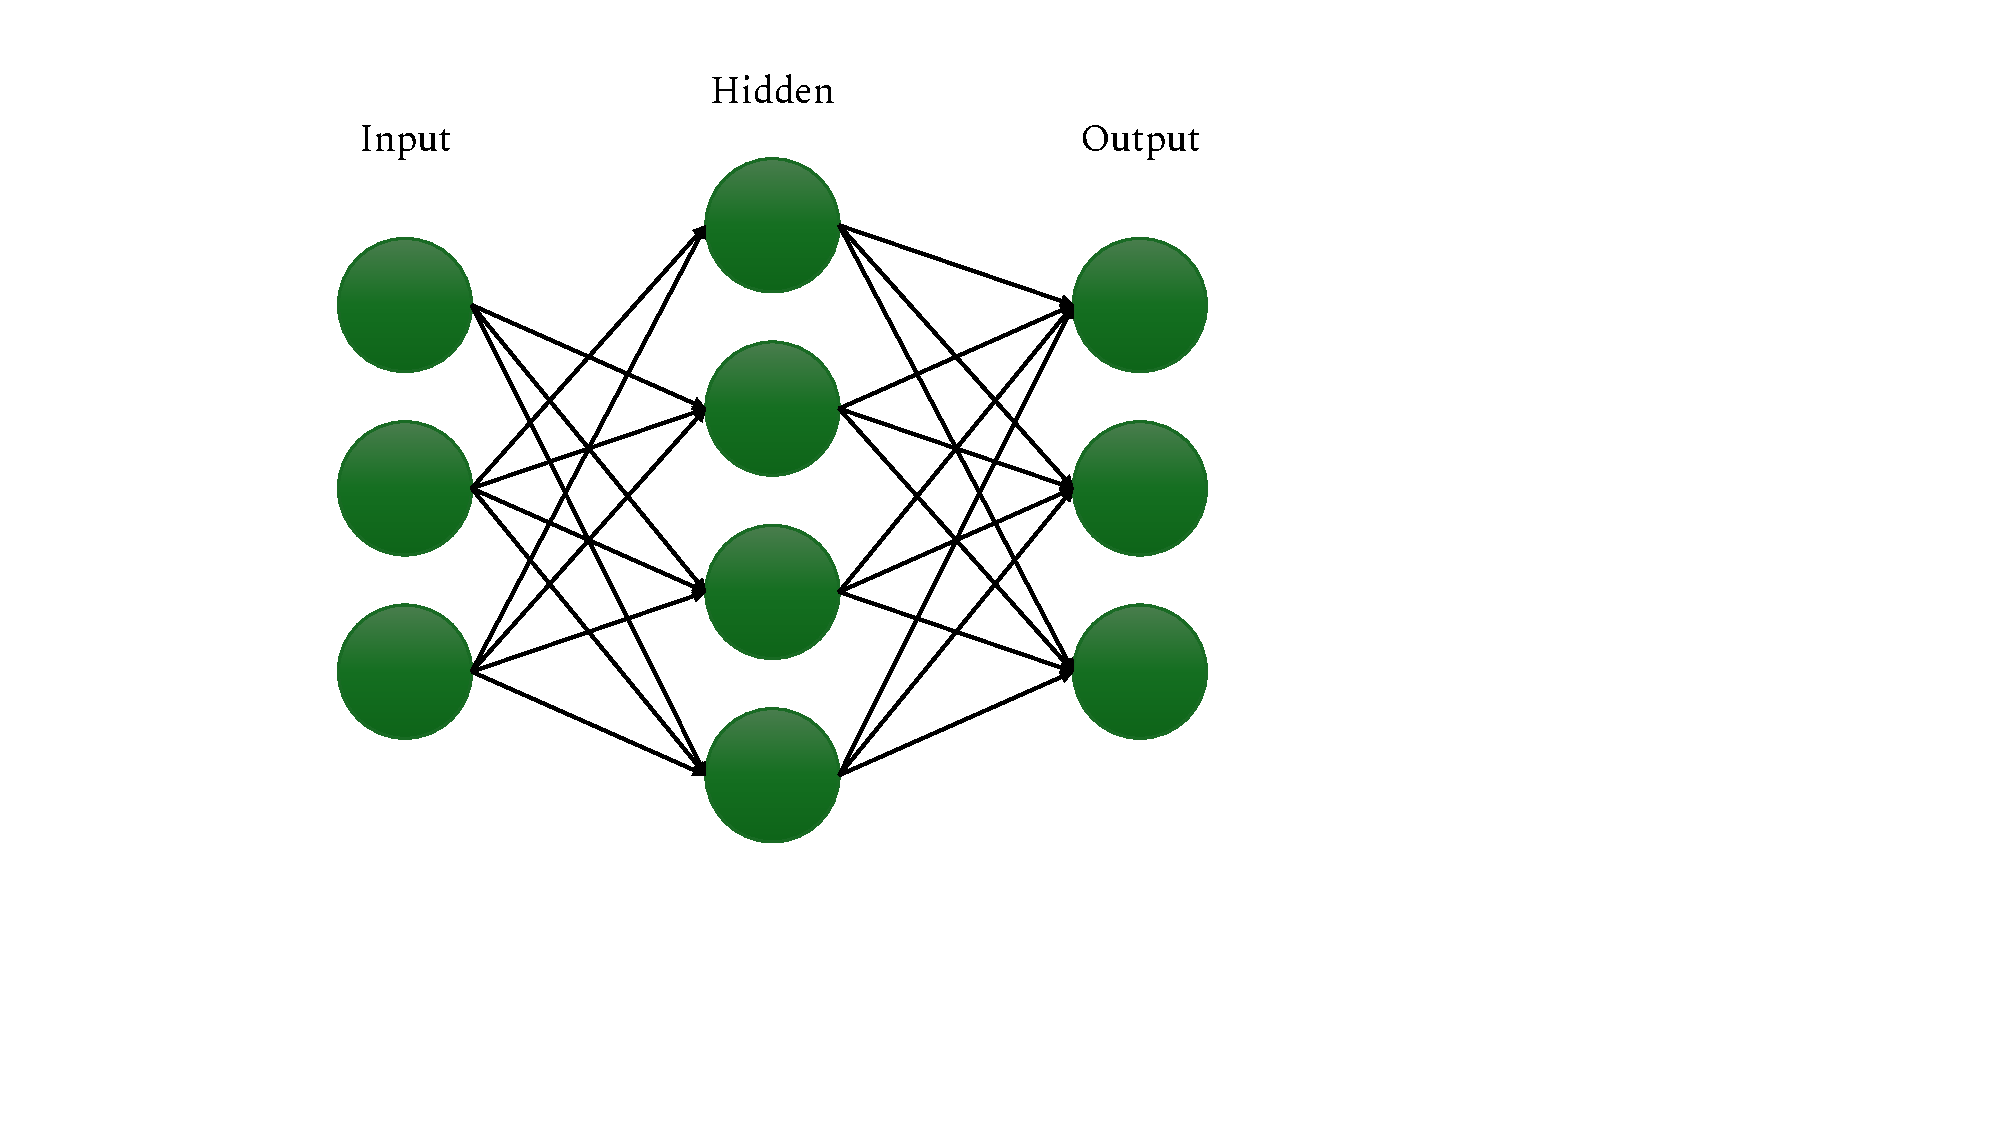
\includegraphics[width=0.6\linewidth,height=\textheight,keepaspectratio]{Chapters/Introduction/Figures/feed-forward neural network visualization.pdf}

}

\end{figure}%

In addition to a feed-forward neural network, the transformer
architecture also implements a self-attention mechanism (see
Figure~\ref{fig-transformermodel}). The self-attention mechanism helps
the model learn which words are related to each other. This attention
mechanism has been the main source of the transformer model's success
over its predecessors. For example, previous models such as Long-Short
Term Memory (LSTM) models or Recurrent Neural Network (RNN) models
struggled with long-term dependencies
(\citeproc{ref-al-selwiLSTMInefficiencyLongterm2023}{Al-Selwi et al.,
2023}; \citeproc{ref-bengioProblemLearningLongterm1993}{Bengio et al.,
1993}). The self-attention mechanism was proposed as a solution to this
limitation.

The self-attention mechanism is a way to quantify which words are most
related to each other. Specifically, the self-attention mechanism
computes the strength of the relationship of each pair of words in the
sentences (\citeproc{ref-vaswaniAttentionAllYou2017}{Vaswani et al.,
2017}). Thus in the sentence, \emph{the students are very bright}, the
self-attention mechanism would assign a high value to the pair
\{\emph{students, are\}} because the word \emph{students} is very
relevant for predicting \emph{are} (as opposed to \emph{is}).\footnote{More
  accurately, Transformer models typically have many different attention
  heads, each of which learns different relationships between words. For
  example, one attention head may attend to determiners of nouns while
  another may attend to objects of prepositions
  (\citeproc{ref-clark2019whatdoesbert}{K. Clark et al., 2019}). While
  there is no guarantee that the weights of these attention heads are
  human-interpretable, fortunately it seems that often times they are
  (\citeproc{ref-clark2019whatdoesbert}{K. Clark et al., 2019}).} This
example is visualized in Figure~\ref{fig-attentionplot} using BERT. For
a more in-depth explanation of attention heads, we direct readers to the
original paper, Vaswani et al.
(\citeproc{ref-vaswaniAttentionAllYou2017}{2017}).

\begin{figure}[htbp]

\caption{\label{fig-attentionplot}A visualization of key-query attention
values for BERT at layer 3, attention head 8. Notice that the strength
between `students' and `are' is high. Brighter colors denote larger
attention weights, darker colors denote smaller attention weights.}

\centering{

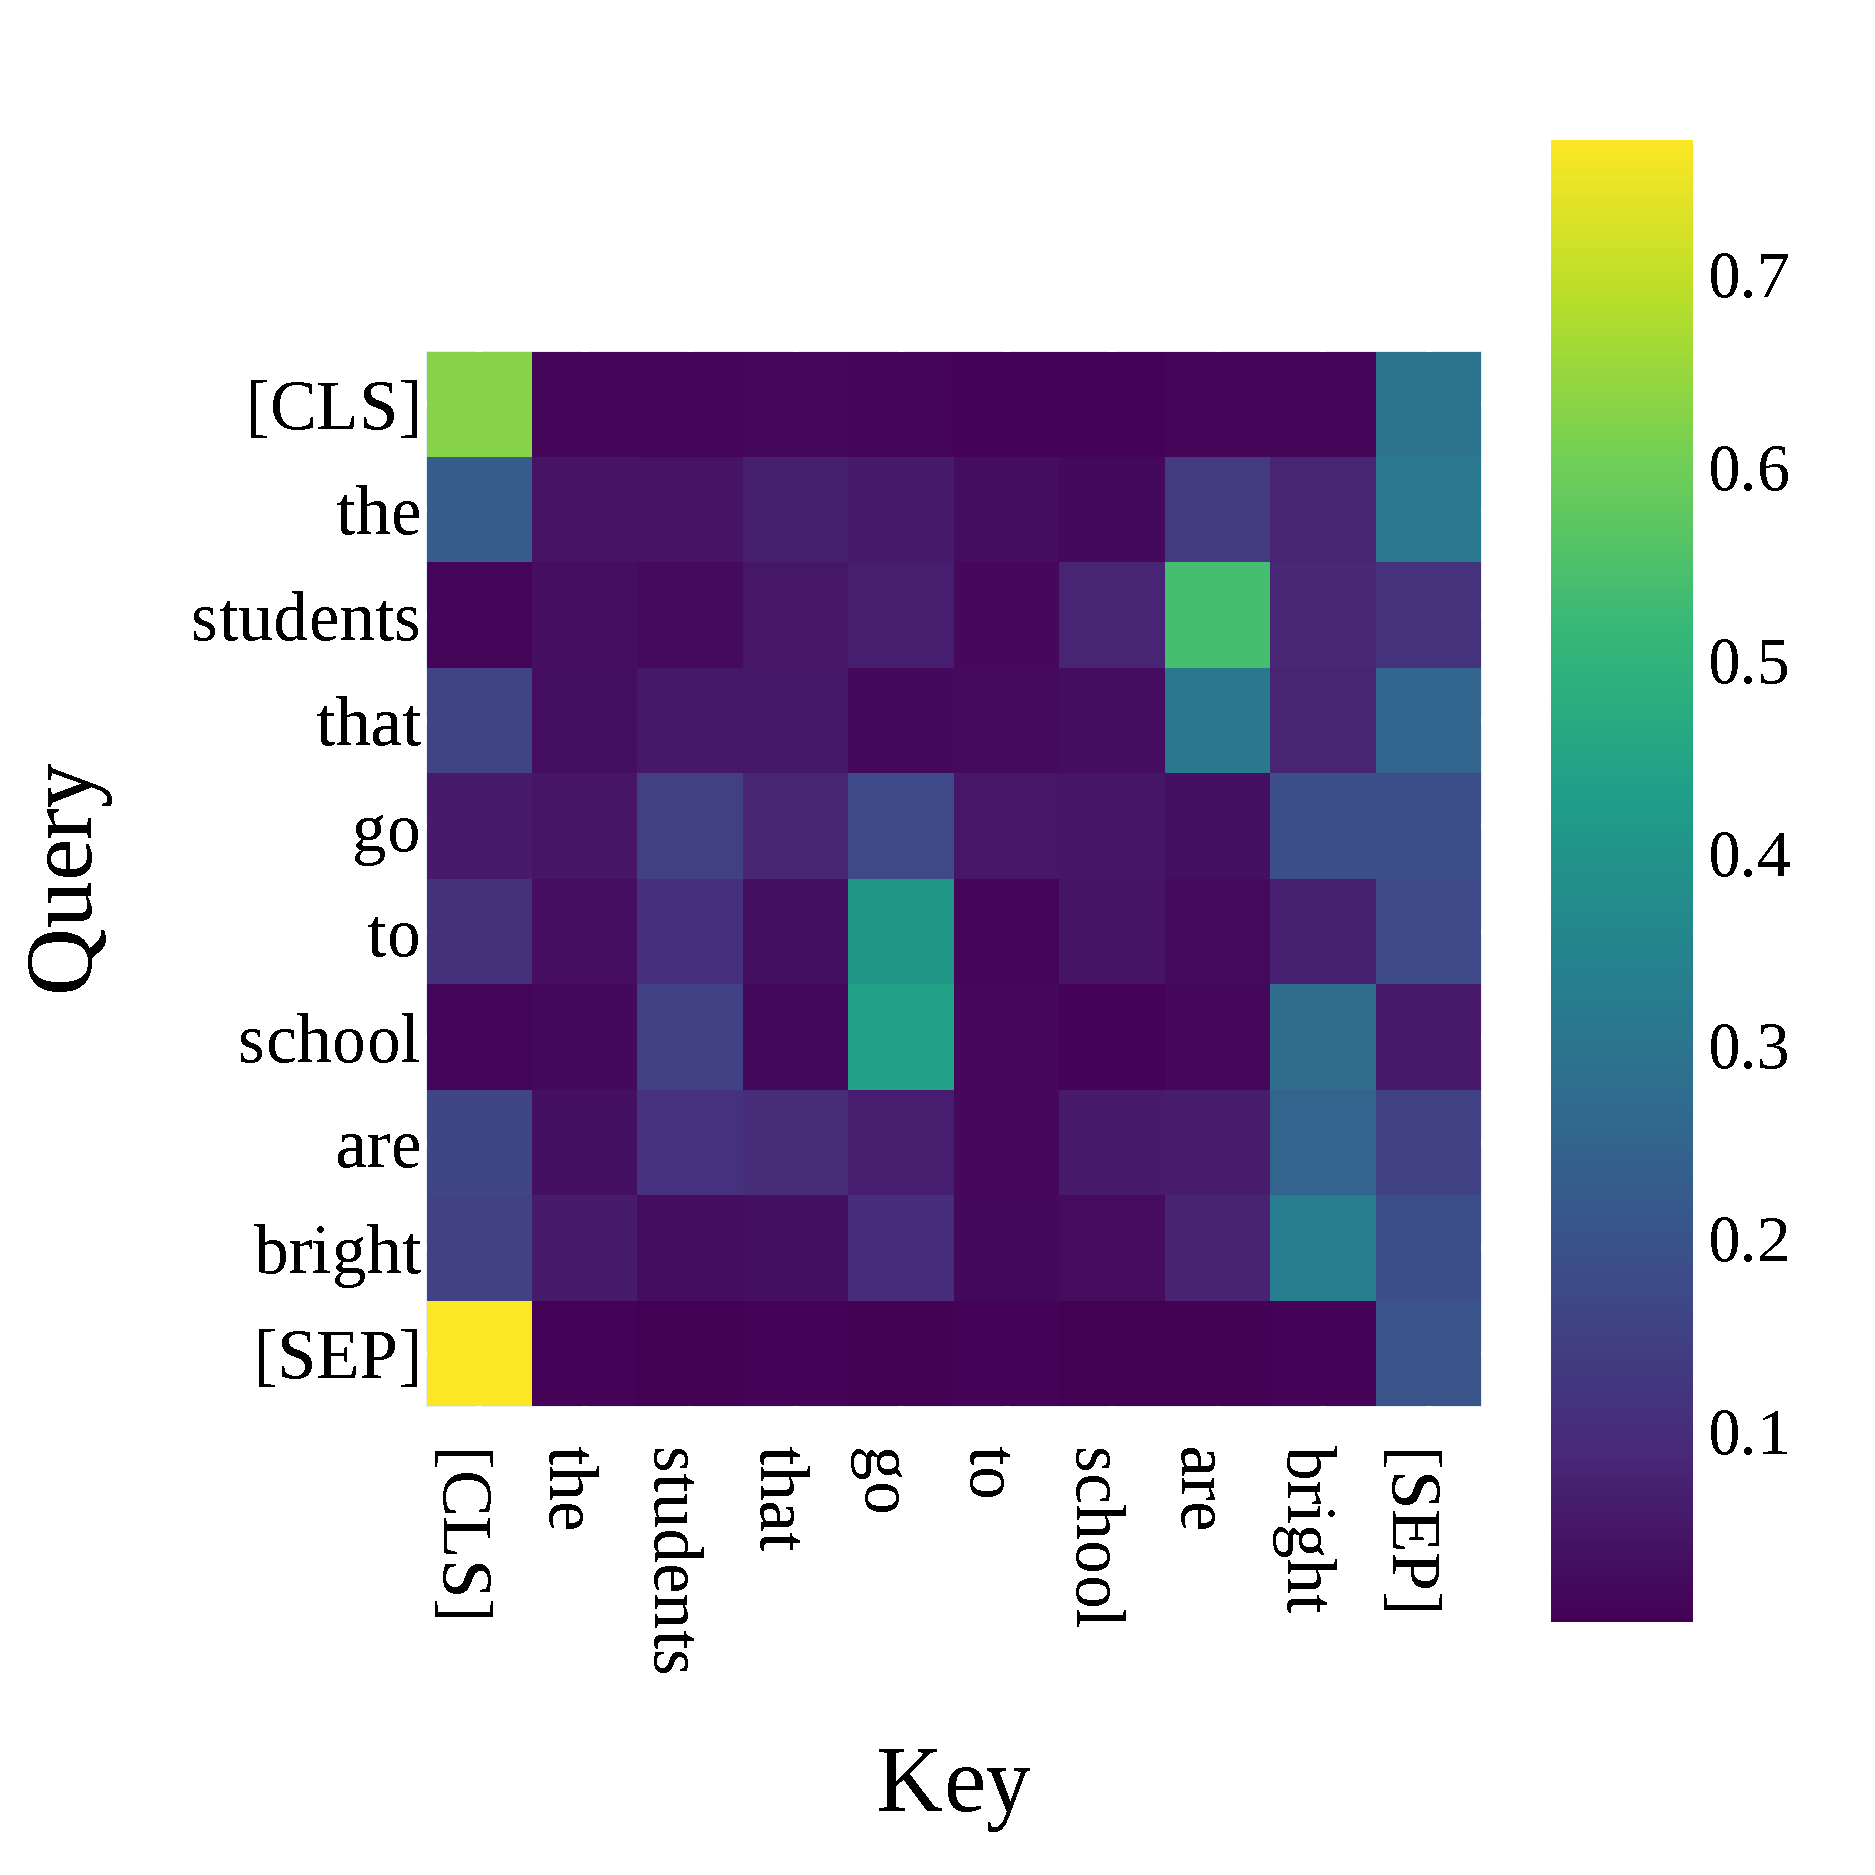
\includegraphics[width=0.5\linewidth,height=\textheight,keepaspectratio]{Chapters/Introduction/Figures/attention_plot.pdf}

}

\end{figure}%

\begin{figure}[t]

\caption{\label{fig-transformermodel}The transformer model architecture,
reproduced from Vaswani et al.
(\citeproc{ref-vaswaniAttentionAllYou2017}{2017}).}

\centering{

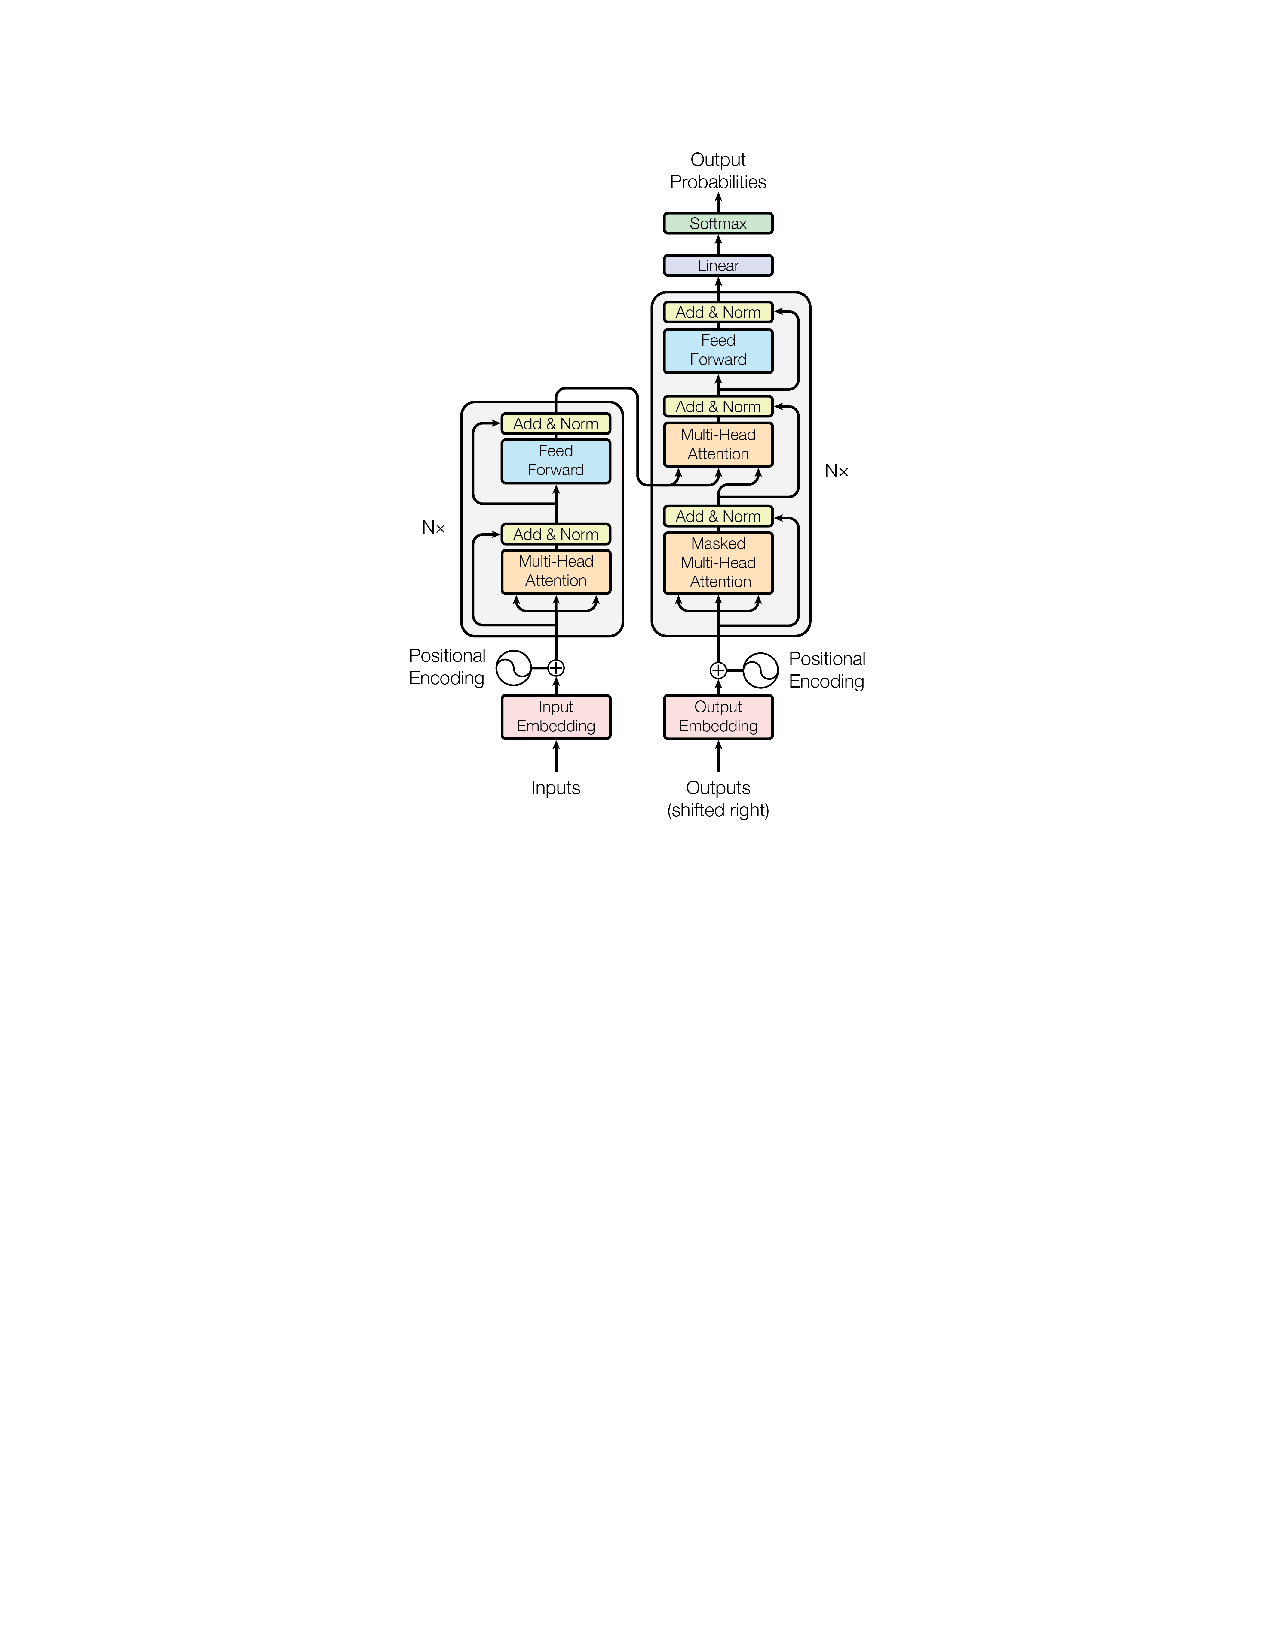
\includegraphics[width=0.6\linewidth,height=\textheight,keepaspectratio]{Chapters/Introduction/Figures/transformer-architecture.pdf}

}

\end{figure}%

\subsection{Lessons from Transformer
Models}\label{lessons-from-transformer-models}

Transformer models have achieved state-of-the-art performance on many
benchmarks and are undoubtedly able to produce fluent, human-like text.
However, it remains unclear to what extent they do this in a human-like
manner. Specifically, how much are these models simply memorizing their
training data as opposed to learning something more abstract about the
language?

For example, there have been doubts about whether they're capable of
learning anything abstract, such as meaning (e.g.,
\citeproc{ref-benderDangersStochasticParrots2021}{Bender et al., 2021}).
Bender \& Koller (\citeproc{ref-bender2020climbingnlumeaning}{2020})
argued that language models cannot learn meaning because they are
trained on only the form of the language. They operationalized meaning
as the relationship between form and communicative intent. However, as
Piantadosi \& Hill
(\citeproc{ref-piantadosiMeaningReferenceLarge2022}{2022}) stated in
their rebuttal, this view of meaning ignores a well-known aspect of
human language: meaning is not as simple as an association between a
form and a referent. For example, the meaning \emph{justice} has no
real-world referent. Instead, people learn these abstract words through
their relationship with other words. This type of learning is something
that large language models do well
(\citeproc{ref-piantadosiChapterModernLanguage}{Piantadosi, 2023}).

Additionally, while there have been many arguments that large language
models don't learn in a human-like manner
(\citeproc{ref-benderDangersStochasticParrots2021}{Bender et al., 2021};
\citeproc{ref-bender2020climbingnlumeaning}{Bender \& Koller, 2020}), it
is rather unclear what is meant by this statement. On one hand it is the
case that large language models are often trained on trillions of tokens
(e.g., \citeproc{ref-groeneveldOLMoAcceleratingScience2024}{Groeneveld
et al., 2024}), which is magnitudes larger than humans who have heard an
average of 350 million words by the time they enter college
(\citeproc{ref-levyProcessingExtraposedStructures2012}{Levy et al.,
2012}). This is further complicated by the fact that a lot of the
training data for high-end large language models is either not
open-access, or so huge that it is difficult to work with. On the other
hand, it is hard to compare the input that a language model receives to
the input that humans receive. While it is true that the number of
tokens that large language models receive is magnitudes larger than
humans, humans receive a lot of contextual information when they hear a
word in the form of sensory information from their environment. It could
be the case that this makes learning in large language models
impossible, or it could be the case that it just requires more data for
them to learn. Given the performance of large language models, the
latter case seems plausible.

Further, the argument that the learning mechanisms in humans and large
language models are completely different also falls apart quite quickly.
Large language models, as was explained in the previous section, learn
from prediction error. They update their representations to maximize
prediction of the upcoming token
(\citeproc{ref-vaswaniAttentionAllYou2017}{Vaswani et al., 2017}).
Learning theories (\citeproc{ref-kapatsinski2018}{Kapatsinski, 2018},
\citeproc{ref-kapatsinskiDefragmentingLearning2023}{2023}; e.g.,
\citeproc{ref-rescorlaProbabilityShockPresence1968}{Rescorla, 1968};
\citeproc{ref-rescorla1972theorypavlovianconditioning}{Rescorla, 1972})
have made the same argument for quite some time, arguing that humans and
animals are sensitive to the probability of upcoming events. Further,
the language processing literature has also demonstrated that humans are
actively predicting upcoming linguistic information
(\citeproc{ref-bansal2018functionfailuresensory}{Bansal et al., 2018};
\citeproc{ref-clark2013arewepredictive}{A. Clark, 2013};
\citeproc{ref-ferreira2018integrationpredictionlanguage}{Ferreira \&
Chantavarin, 2018}; \citeproc{ref-kuperberg2016whatwemean}{Kuperberg \&
Jaeger, 2016};
\citeproc{ref-olejarczukDistributionalLearningErrordriven2018}{Olejarczuk
et al., 2018};
\citeproc{ref-ramscarChildrenValueInformativity2013}{Ramscar et al.,
2013}). This isn't to say that language models are learning identically
to humans, but rather that there is enough overlap between large
language models and humans to warrant a close examination of them. In
fact, understanding the differences between humans and large language
models may be a fruitful endeavor, leading to improvements in both
language models as well as theories of language.

Thus in this section we take a closer examination into what evidence
there is that language models are learning something meaningful about
the language as opposed to simply memorizing their training data.

First, there is evidence that large language models do copy a
significant amount from their training. For example, Haley
(\citeproc{ref-haleyThisBERTNow2020}{2020}) demonstrated that many of
the BERT models are not able to reliably determine the correct plural
form for novel words. Specifically, he tested BERT on English, French,
Dutch, and Spanish on a number-agreement task. He evaluated whether the
model was able to predict the correct plural form of novel-words in a
no-prime condition and a prime-condition, where a previous sentence
reveals the correct form of the verb (as well as the appropriate gender
for the languages with a gender distinction). Humans are able to
reliably use the prime to form the correct plural even for non-words.
Interestingly, they found that BERT was not able to reliably use the
prime to improve performance on the non-words.

Similarly, Li \& Wisniewski
(\citeproc{ref-liAreNeuralNetworks2021}{2021}) demonstrated that BERT
relies on memorization when producing the correct tense for a word as
opposed to learning a more general linguistic pattern. They examined the
ability of BERT to learn the correct tense in French and Chinese and
found that while BERT is able to do well in French, it does much worse
in Chinese. They argued that this is because while in French the correct
tense information is expressed in the verb morphology (and can therefore
be predicted by surface statistics of the language), in Chinese tense is
driven by a variety of different cues, including abstract, lexical,
syntactic, and pragmatic information. The poor performance in Chinese
thus, according to the authors, suggests that BERT relies on
memorization of surface-level statistics.

There is also a substantial amount of evidence that language models are
learning more general patterns of the language
(\citeproc{ref-lasriSubjectVerbAgreement2022}{Lasri et al., 2022};
\citeproc{ref-liAssessingCapacityTransformer2023}{Li et al., 2023};
\citeproc{ref-liAreNeuralNetworks2021}{Li \& Wisniewski, 2021};
\citeproc{ref-mccoyHowMuchLanguage2023}{McCoy et al., 2023};
\citeproc{ref-misraLanguageModelsLearn2024}{Misra \& Mahowald, 2024};
\citeproc{ref-weissweilerLinguisticGeneralizationsAre2025}{Weissweiler
et al., 2025}; \citeproc{ref-yaoBothDirectIndirect2025}{Yao et al.,
2025}). For example, Lasri et al.
(\citeproc{ref-lasriSubjectVerbAgreement2022}{2022}) examined whether
BERT is able to use the correct inflection of verbs in semantically
incoherent contexts (e.g., \emph{colorless green ideas sleep
furiously}). They found that while BERT does do worse when the context
is semantically incoherent, the decrease in performance is comparable to
the decrease we see in humans. Additionally, Li et al.
(\citeproc{ref-liAssessingCapacityTransformer2023}{2023}) examined
BERT's performance on subject-verb and object-past agreements in French.
They used a probing task to determine whether the model learned anything
general about the language. The probing task attempted to predict the
number of the verb and the object-past agreements from the
representations in the model. Their probe achieved a high accuracy,
suggesting that the model encoded an abstract representation for these
linguistic features.

The evidence for abstractions is not limited to BERT, either. There is
also evidence that other transformer models can learn more abstract
knowledge as well. For example, McCoy et al.
(\citeproc{ref-mccoyHowMuchLanguage2023}{2023}) examined the text that
GPT-2 produces in relation to its training data. They found that while
GPT-2 does copy a great deal, it also produces both novel words and
syntactic structures.

In addition to large language models, more recently there has been an
interesting line of research examining language models trained on a more
human amount of data. For example, Misra \& Mahowald
(\citeproc{ref-misraLanguageModelsLearn2024}{2024}) demonstrated that a
language model trained on the BabyLM-strict corpus (a corpus containing
a comparable amount of data as humans receive;
\citeproc{ref-warstadtFindingsBabyLMChallenge2023}{Warstadt et al.,
2023}) can learn article-adjective-numeral-noun constructions (AANNs).
AANNs are constructions such as \emph{a beautiful five days}. They occur
relatively infrequently in English but humans still learn develop
preferences for these. For example, while \emph{a beautiful five days}
is perfectly grammatical, \emph{a blue five pencils} is not. They found
that even after removing all AANN occurrences from the training data,
the language model is still able to learn these constructions. They
further demonstrated that this is likely learned from similar
constructions, such as \emph{a few days}. The results of this shows that
even when trained on a comparable amount of data as humans, language
models are still able to learn general patterns in the language.

Similarly, Yao et al. (\citeproc{ref-yaoBothDirectIndirect2025}{2025})
examined how language models learn the dative alternation. The dative
alternation is a common construction in English where one can say either
\emph{give the toy to the cat} or \emph{give the cat the toy}. While
these two constructions have similar meanings, Humans have preferences
for one over the other depending on the length or animacy of each noun
phrase. In order to examine this phenomenon in language models, they
trained a language model on a comparable amount of data to humans.
Crucially they removed dative alternations that contained a length or
animacy bias. They found that while the effect weakens, there is still
an effect of length. They argued that this is evidence that language
models are learning general patterns of the language. These results
taken together with previous results demonstrate the ability of
transformer models to learn general patterns in the language.

However, there is still a lot we don't know. What factors determine
whether models learn general patterns of the language as opposed to
relying on item-specific preferences? For example, humans seem to be
sensitive to a combination of type and token frequency when they
generalize beyond a specific word
(\citeproc{ref-harmonPuttingOldTools2017}{Harmon \& Kapatsinski, 2017}).
Are language models sensitive to similar factors? Further is this
knowledge represented in a similar way as humans? That is, are the
general preferences that large language models learn similar to those
that humans learn? Understanding the answers to these questions is
important for evaluating these models as theories of human language
learning.

\section{Outline of Dissertation}\label{sec-outline-of-dissertation}

In the present dissertation, we provide an in depth examination of how
humans trade off between storage and computation. In the next chapter,
we examine whether predictability drives storage and how holistic
representations are accessed. In Chapter 3, we examine how holistically
stored items are represented. Chapter 4 examines how large language
models trade off between storage and computation. Chapter 5 examines how
stored items are represented in the embeddings of large language models.
Finally, Chapter 6 examines whether storage accounts can explain
frequency-dependent preference extremity.\footnote{All data and code for
  this dissertation can be found in the following github repository:
  \url{https://github.com/znhoughton/dissertation_writeup}.}

\bookmarksetup{startatroot}

\chapter{Does Predictability Drive the Holistic Storage of Compound
Nouns?}\label{does-predictability-drive-the-holistic-storage-of-compound-nouns}

\section{Introduction}\label{introduction-1}

Learning a language is not a trivial task. In order to be successful,
learners must accurately segment the continuous speech stream into
smaller segments, including phrases, words, morphemes, and phonemes. One
of the main questions that arises out of this task is what exactly is
the size of the units that learners are storing. That is, are they
storing individual words, entire sentences, phrases, or some combination
of all of these? One possibility is that learners store very little
outside of words and idioms. For example, traditional theories have
argued that learners don't store any more than they need to: they store
only what they can't form compositionally using a set of rules, and
generate everything else (e.g., \citeproc{ref-chomsky1965}{Chomsky,
1965}). According to these theories, inflected words, such as
\emph{walked} would be generated by accessing the stored root,
\emph{walk}, and then applying a past tense rule that generates
\emph{walked} from the root. Similarly, a phrase like \emph{I don't
know} would be generated by accessing each of the individually stored
words \emph{I}, \emph{don't}, and \emph{know}.

On the opposite side of this theoretical spectrum, it's also possible
that learners store everything, including entire sentences. Ambridge
(\citeproc{ref-ambridgeStoredAbstractionsRadical2020}{2020}) argued for
exactly this, specifically arguing that everything a learner hears ``is
stored with its meaning, as understood in that individual situation''
and that unwitnessed novel-forms are produced using on-the-fly analogy
across stored exemplars Ambridge
(\citeproc{ref-ambridgeStoredAbstractionsRadical2020}{2020}). For
example, producing a novel plural form, like \emph{wugs}, would consist
of analogizing (on-the-fly) over multiple stored exemplars (e.g.,
\emph{cats}, \emph{chairs}, \emph{dogs}, etc).

It is also possible that what gets stored is somewhere in between these
two extremes. For example, usage-based construction grammar approaches
have posited that a lot more than just words are stored -- including
high-frequency phrases -- but rather than storing everything, or storing
only the most basic units, instead humans store units of varying size
depending on usage-based factors such as frequency
(\citeproc{ref-arnonMoreWordsFrequency2010}{Arnon \& Snider, 2010};
\citeproc{ref-baayenAmorphousModelMorphological2011}{R. H. Baayen et
al., 2011}; \citeproc{ref-bybee2003}{Bybee, 2003};
\citeproc{ref-bybee2001}{Bybee \& Hopper, 2001};
\citeproc{ref-goldbergConstructionsNewTheoretical2003}{Goldberg, 2003};
\citeproc{ref-morgan2015}{Morgan \& Levy, 2015},
\citeproc{ref-morganAbstractKnowledgeDirect2016}{2016a},
\citeproc{ref-morgan2024}{2024};
\citeproc{ref-odonnellProductivityReuseLanguage2016}{O'Donnell, 2016};
\citeproc{ref-tomaselloConstructingLanguageUsagebased2005}{Tomasello,
2005}). That is to say, the size of the units stored is driven by the
statistical distribution of the language that the learner is producing
and perceiving. For example, Bybee (\citeproc{ref-bybee2003}{2003}) drew
an analogy to learning to play a piece on the piano:

\begin{quote}
An important result of learning to play several pieces is that new
pieces are then easier to master. Why is this? I hypothesize that the
player can access bits of old stored pieces and incorporate them into
new pieces. The part of a new piece that uses parts of a major scale is
much easier to master if the player has practiced scales than is a part
with a new melody that does not hearken back to common sequences. This
means that snatches of motor sequences can be reused in new contexts.
The more motor sequences stored, the greater ease with which the player
can master a new piece (\citeproc{ref-bybee2003}{Bybee, 2003, pp.
14--15}).
\end{quote}

\noindent In this same line of thinking, Bybee
(\citeproc{ref-bybee2003}{2003}) further argued against a strictly
traditional view, stating that learning the English past tense
\emph{-ed} requires learning a series of words that contain that segment
(e.g., \emph{played}, \emph{spilled}, \emph{talked}) and that these are
not necessarily flushed from memory after learning the English past
tense marker.

There is no shortage of evidence for the holistic storage of multi-word
phrases. For example, high-frequency phrases, such as \emph{I don't
know}, have been shown to undergo phonetic reduction that isn't seen in
other low or mid-frequency phrases containing \emph{don't}
(\citeproc{ref-bybeeEffectUsageDegrees1999}{Bybee \& Scheibman, 1999})
suggesting that the representation of \emph{I don't know} is separate
from the representation of each of the individual words. In other words,
the susceptibility of high-frequency phrases to phonological change is
strong evidence that they may come to have a mental representation for
the whole expression (i.e., holistic storage). This example is not an
outlier either, there are many examples of high-frequency phrases
undergoing phonetic reduction: \emph{going to}, want to\emph{, have to},
etc (\citeproc{ref-bybee2003}{Bybee, 2003}). Additionally, in Korean, Yi
(\citeproc{ref-yiEumun2002}{2002}) demonstrated that in multi-word
phrases containing the adnominal future marker (\emph{-l}), the
tensification of the consonant following the adnominal is predicted by
the phrasal frequency. That is, in high-frequency phrases, consonants
following the adnominal became tense at a higher rate than in
low-frequency phrases.\footnote{A similar effect has been demonstrated
  on the word-level as well in Korean, where epenthesis has been
  documented to occur more often in high-frequency words than in
  low-frequency words
  (\citeproc{ref-leeFrequencyEffectsMorphologisation2015}{Lee \&
  Kapatsinski, 2015}). This suggests that there may not be a clear
  division between the representation of high-frequency phrases and
  high-frequency words.}

Evidence for holistic storage is not limited to phonological effects,
either. In the Psycholinguistics literature, Siyanova-Chanturia et al.
(\citeproc{ref-siyanova-chanturiaSeeingPhraseTime2011}{2011})
demonstrated that readers are sensitive to the ordering of binomials in
English. In an eye-tracking experiment, participants read frequent
binomial expressions in English in their preferred order (e.g.,
\emph{bride and groom}) and their reversed order (\emph{groom and
bride}). They found that the preferred orderings were read faster.
Further, Morgan \& Levy
(\citeproc{ref-morganAbstractKnowledgeDirect2016}{2016a}) investigated
whether the results from Siyanova-Chanturia et al.
(\citeproc{ref-siyanova-chanturiaSeeingPhraseTime2011}{2011}) could be
attributed to abstract knowledge of binomial orderings (e.g., a
preference for male names before female names) or whether they were due
to participants' direct experience with those items (e.g., hearing one
ordering of a specific binomial more often than the complementary
ordering). They developed a probabilistic model to approximate native
English speakers' ordering preferences and combined that with a
forced-choice and a self-paced reading task in order to investigate
whether ordering preferences were driven by abstract knowledge or direct
experience of the expression. They found that reading times for frequent
binomials were influenced only by relative frequency (i.e., direct
experience), not abstract knowledge. That is to say, ordering
preferences of frequent binomials weren't explained by abstract ordering
preferences, but rather by linguistic experience with the specific
binomial, suggesting that high-frequency binomials are stored
holistically.

Similarly, O'Donnell
(\citeproc{ref-odonnellProductivityReuseLanguage2016}{2016}) tested 4
probabilistic models on their ability to learn the English past tense
and derivational morphology. Specifically, they tested a Full-parsing
model, which stores minimal-sized units only, a Full-listing model,
which stores the entirety of units only, an Exemplar-based model, which
stores all units and all sub-units consistent with the data, and finally
a Productivity as an Inference model, which, similar to the
Exemplar-based Inference model, can store both smaller and larger
structures, but probabilistically determines which items to store based
on the data. They found that the Inference-based model performed the
best overall for both past tenses and derivational morphology. In other
words, storing units of varying sizes (as opposed to just minimal or
maximal-sized units) seems to be the most conducive to learning the
various morphological paradigms in English.

Despite the clear evidence for the holistic storage of some multi-word
units, however, it is still largely unclear what determines whether a
unit is stored holistically. For example, it is possible that storage is
driven by either \textbf{phrasal frequency}
(\citeproc{ref-bybee2001}{Bybee \& Hopper, 2001}) or by the mutual
\textbf{predictability} of a phrase's component parts (i.e., how
predictable the whole phrase is from part of the phrase;
\citeproc{ref-odonnellProductivityReuseLanguage2016}{O'Donnell, 2016}).
For example, as previously stated, there is an abundance of evidence
that high-frequency phrases are more susceptible to phonetic reduction
than low-frequency phrases (\citeproc{ref-bybee2003}{Bybee, 2003};
\citeproc{ref-bybeeEffectUsageDegrees1999}{Bybee \& Scheibman, 1999}).
Additionally, high-frequency phrases have been shown to lose the
recognizability of their component parts relative to low-frequency
phrases
(\citeproc{ref-kapatsinskiFrequencyEmergencePrefabs2009}{Kapatsinski \&
Radicke, 2009}). For example, \emph{up} is harder to recognize in
\emph{pick up} than in \emph{run up}. On the other hand, in the learning
literature, there is significant evidence that learning is driven by
prediction error as opposed to raw co-occurrence statistics. For
example, Ramscar et al.
(\citeproc{ref-ramscarChildrenValueInformativity2013}{2013})
demonstrated that in word learning, children rely on more than simple
co-occurrence statistics but also on how \emph{informative} -- that is,
how \emph{predictive} -- a cue is of an outcome (relative to other
cues). Specifically, they demonstrated that children rely on not only
co-occurrence rate, but also background rate (how often a cue is present
without an outcome). In other words, assuming doors have a higher
co-occurrence rate and lower background rate than all the other
competing cues (e.g., brown, house, room) for the word \emph{door}, then
children will learn that doors are the best predictor of the word
\emph{door}
(\citeproc{ref-ramscarChildrenValueInformativity2013}{Ramscar et al.,
2013}).

A similar debate persists in the speech perception literature, where
Pierrehumbert
(\citeproc{ref-pierrehumbertExemplarDynamicsWord2001}{2001}) argued that
internal representations reflect the raw frequency distribution of the
input. On the other hand, Olejarczuk et al.
(\citeproc{ref-olejarczukDistributionalLearningErrordriven2018}{2018})
argued that the learning of phonemes is driven not by co-occurrence
statistics (i.e., raw frequency), but rather by surprisal (i.e.,
prediction error). In other words, learners are actively predicting
upcoming phonemes and update their beliefs in proportion to how
surprising the upcoming phoneme is. Thus the debate between
co-occurrence vs predictability in the role of learning is not unique to
the word learning literature.

Additionally, if learners are storing more than just single-word units,
what are the processing consequences of this? For example, as mentioned
earlier, Kapatsinski \& Radicke
(\citeproc{ref-kapatsinskiFrequencyEmergencePrefabs2009}{2009})
investigated the recognition of the particle \emph{up} in phrases of
varying frequencies and found that the recognition of the particle
\emph{up} is significantly more difficult in a high-frequency phrases
than in low-frequency phrases, suggesting that high-frequency units
`fuse' together, losing some of the recognizability of their individual
parts.

On the other hand, Staub et al.
(\citeproc{ref-staubTimeCoursePlausibility2007}{2007}) investigated the
effects of plausibility on the reading times of familiar and novel
compound nouns, which were compound nouns with high and low phrasal
frequency respectively. Participants read sentences which contained a
novel compound noun or a familiar compound noun (See Example
\ref{staubitems}) in a plausible condition (e.g., Example
\ref{novelplaus}) or an implausible condition (e.g., Example
\ref{novelimplaus}). Crucially, the second noun in the compound
eliminated the local implausibility such that every sentence was
plausible after reading the second noun. For example, in
\ref{novelimplaus}, \emph{The zookeeper spread out the monkey\ldots{}}
is locally implausible, however upon reading the second noun in the
compound, \emph{medicine}, the local implausibility is eliminated.

\begin{exe}
\ex \label{staubitems}
\begin{xlist}
\ex Novel Compound \label{compound}
\begin{xlist}
\ex The zookeeper picked up the monkey medicine that was in the enclosure. \hfill \emph{plausible} \label{novelplaus}
\ex The zookeeper spread out the monkey medicine that was in the enclosure. \hfill \emph{implausible}\label{novelimplaus}
\end{xlist}
\ex Familiar Compound
\begin{xlist}
\ex Jenny looked out on the huge mountain lion pacing in its cage. \hfill \emph{plausible}\label{familiarplaus}
\ex Jenny heard the huge mountain lion pacing in its cage. \hfill \emph{implausible} \label{familiarimplaus}
\end{xlist}
\end{xlist}
\end{exe}

\noindent They found that the size of the plausibility effect was the
same for both novel and familiar compound nouns. That is to say, while
familiar items were read more quickly than novel items, and there was an
increase in reading times in the implausible condition, the size of the
plausibility effect was not different for familiar items (relative to
novel items). However, if familiar items are stored holistically, one
might expect that readers would predict the second noun upon reading the
first, thus eliminating the local implausibility. Thus, if these items
are stored holistically it begs the question of what the processing
consequences of storage are. On the other hand, it may just be that
these items are not stored. For example, it is possible that, as has
been previewed throughout the introduction, phrasal frequency may not be
the driving factor of storage and that it is actually predictability
that might be driving storage. If this is the case, then it is possible
that the reason for a lack of an interaction effect in Staub et al.
(\citeproc{ref-staubTimeCoursePlausibility2007}{2007})'s results is due
to their stimuli being low-predictability compound nouns. For example,
while \emph{mountain lion} has a high phrasal frequency, \emph{mountain}
is not very predictable of \emph{lion} (that is, the probability of
\emph{lion} following \emph{mountain} is fairly low, despite the overall
phrase having a relatively high-frequency).

Thus there are two main problems that the present study aims to provide
insight on: what exactly drives holistic storage, and what are the
processing consequences of storage? In Experiment 1, we first replicate
Staub et al. (\citeproc{ref-staubTimeCoursePlausibility2007}{2007})'s
experiment using a maze task (\citeproc{ref-boyceMazeMadeEasy2020}{Boyce
et al., 2020}). In Experiment 2, we use the same methodology, but
instead of using high (phrasal) frequency compound nouns, we use
high-\emph{predictability} compound nouns (e.g., \emph{peanut butter}).
By using the highest predictability compound nouns from the Google
\emph{n}-grams corpus
(\citeproc{ref-michel2011quantitativeanalysisculture}{Michel et al.,
2011}), we ask whether the difference in reaction times between the
locally implausible and plausible contexts differs depending on whether
the compound noun is highly predictable or not. For example, if highly
predictable compound nouns are stored holistically, it is possible that
when listeners hear, or read, the first noun in a highly predictable
compound noun they may access the second noun as well and/or a holistic
compound noun representation. If this is the case, then locally
implausible contexts should not incur as much processing difficulty when
the compound noun is highly predictable because the second noun
eliminates the local implausibility. Lastly in Experiments 3 and 4 we
replicate these with eye-tracking.

\section{Experiment 1}\label{experiment-1}

\subsection{Methods}\label{methods}

\subsubsection{Participants}\label{participants}

Participants were presented with sentences online via ibex farm, a
web-based experiment software platform that is freely-available
(\url{github.com/addrummond/ibex}) and were recruited through the
University of California Linguistics/Psychology Human Subjects Pool. To
prevent selection bias, participants signed up for the experiment
blindly, without knowledge of the content of the experiment. 146
participants were recruited, however 30 participants were excluded for
having an overall accuracy below 70\% (in this case, accuracy is
operationalized as choosing the correct word; an inaccuracy would be
choosing the ungrammatical distractor word), leaving a total of 116
participants. All participants self-reported being native English
speakers.

\subsubsection{Stimuli}\label{stimuli}

The experimental sentences were sentences containing compound nouns from
(\citeproc{ref-staubTimeCoursePlausibility2007}{Staub et al., 2007})
which varied upon two dimensions: local plausibility and familiarity.
Locally plausible sentences were sentences in which the reading at the
first noun was plausible and locally implausible sentences were
sentences in which the reading at the first noun in the compound was
implausible (see example sentences \ref{novelimplaus} and
\ref{familiarimplaus}). Local plausibility was a within-item effect and
familiarity (the frequency of the compound noun) was a between-item
effect. The sentences in \ref{staubitems} above exemplify each
condition: the first sentence in each is locally plausible while the
second one is locally implausible. For example, in sentence
\ref{familiarplaus}, it is semantically plausible that \emph{Jenny
looked out on the huge mountain\ldots{}} but not semantically plausible
that \emph{Jenny heard the huge mountain} (sentence
\textbackslash ref\{familiarimplaus). Altogether, our stimuli consisted
of 24 novel items, 24 familiar items (taken from
\citeproc{ref-staubTimeCoursePlausibility2007}{Staub et al., 2007}), and
188 filler sentences in order to avoid participants discerning the
experimental design.

\subsubsection{Procedure}\label{procedure}

Experiment 1 is a direct replication of Staub et al.
(\citeproc{ref-staubTimeCoursePlausibility2007}{2007}) using the A-Maze
task (\citeproc{ref-boyceMazeMadeEasy2020}{Boyce et al., 2020}) instead
of eye-tracking.\footnote{The maze task was used due to the limitations
  of the COVID-19 pandemic.} In the A-maze task, participants are
presented with the first word in the sentence and then have to correctly
choose between an ungrammatical distractor word and the next word in the
sentence. When participants select the correct word, they continue to
the next word in the sentence until the sentence is finished. The
distractor words for the A-maze were generated automatically following
Boyce et al. (\citeproc{ref-boyceMazeMadeEasy2020}{2020}) using the
Gulordava model Gulordava et al.
(\citeproc{ref-gulordava2018colorlessgreenrecurrent}{2018}). The
locations of the distractor word and target word were counterbalanced so
that they appeared an equal number of times on the left and right side
of the screen. For each word, the reaction time was recorded along with
whether the subject chose the correct item or not. See
Figure~\ref{fig-mazevisualization} for a visualization of the maze task,
reproduced from Boyce et al.
(\citeproc{ref-boyceMazeMadeEasy2020}{2020}).

\begin{figure}[htbp]

\caption{\label{fig-mazevisualization}A visualization of the maze task,
reproduced from Boyce et al.
(\citeproc{ref-boyceMazeMadeEasy2020}{2020}).}

\centering{

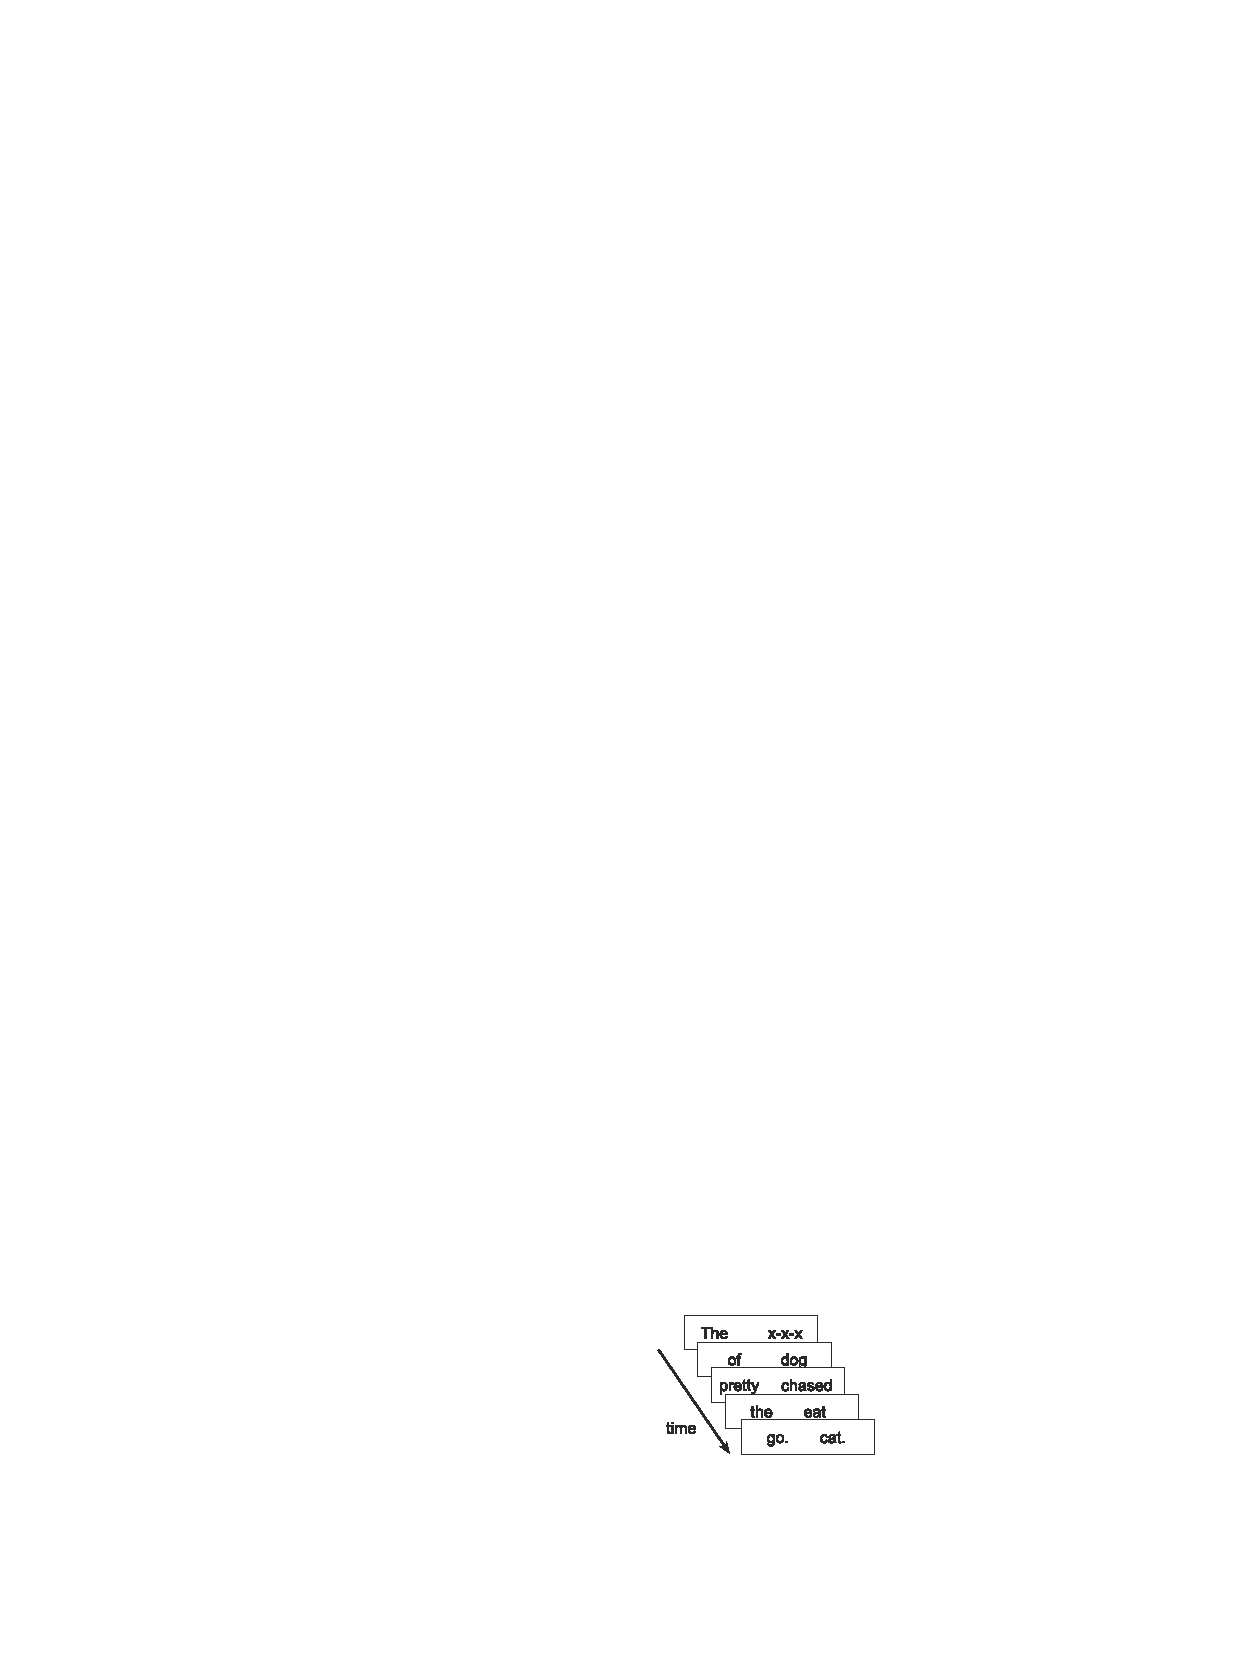
\includegraphics[width=0.5\linewidth,height=\textheight,keepaspectratio]{Chapters/Compound Nouns/Figures/mazevisualization.pdf}

}

\end{figure}%

Sentences were presented in a random order and each word was presented
an equal number of times on the left and right side of the screen.
Additionally, each item appeared an equal number of times in the
implausible and plausible context and no participant was presented with
the same item in more than one condition. The complete dataset included
9994 response tokens.

\subsubsection{Analysis}\label{analysis}

The data was analyzed using Bayesian linear regression models, as
implemented in the \emph{brms} package
(\citeproc{ref-burknerBrmsPackageBayesian2017}{Bürkner, 2017}) within
the R programming environment R Core Team
(\citeproc{ref-Rpackage}{2022}).\footnote{For more details about the
  analyses, our materials are available at the following link:
  \url{https://github.com/znhoughton/dissertation_writeup/tree/master/Chapters/Compound\%20Nouns}.}
We subsetted the data into two sets based on the region: one set for the
first noun in the compound noun and one set for the second noun in the
compound. The primary dependent variable was log reaction time for both
of these regions (following \citeproc{ref-boyceMazeMadeEasy2020}{Boyce
et al., 2020}). The primary independent variables were plausibility and
familiarity (following
\citeproc{ref-staubTimeCoursePlausibility2007}{Staub et al., 2007}). We
modeled reaction time as a function of plausibility and familiarity,
including their interaction, with maximal random effects
(\citeproc{ref-barrRandomEffectsStructure2013}{Barr et al., 2013}). The
formula used for the model is presented in equation
Equation~\ref{eq-modelfamil} below, with \emph{Plaus} as plausibility
and \emph{Famil} as familiarity. All models were sum-coded
\begin{equation}\phantomsection\label{eq-modelfamil}{
Reaction Time \sim Plaus*Famil+(Plaus*Famil|Subject)+(Plaus|Item)
}\end{equation}

\subsection{Results}\label{results}

As mentioned in the methods section, for the purpose of the analysis,
the data was divided into two regions: the N1 region and the N2 region,
which were the first and second noun in the compound noun respectively.
The results of the Bayesian regression model for the N1 region are
presented in Table~\ref{tbl-N1Staub} and in Figure~\ref{fig-N1Staub},
and the results of the N2 region are presented in
Table~\ref{tbl-N2Staub} and in Figure~\ref{fig-N2Staub}.

For the N1 region, there was an increase in reaction time for the
implausible condition relative to the plausible condition. There was no
such effect for familiarity. In other words, while participants took
longer selecting the correct word in the implausible condition, their
reaction times were not affected by the familiarity of the compound
noun. This is expected given that the familiarity condition was not the
frequency of the first noun, but rather the frequency of the compound
noun as a whole. Additionally, there was no interaction effect between
plausibility and familiarity.

Following Wagenmakers et al.
(\citeproc{ref-wagenmakers2010bayesianhypothesistesting}{2010}), a
post-hoc Bayes factor analysis was conducted to compare the interaction
effect to the null hypothesis (interaction effect = 0). We found a Bayes
Factor value of 18.15 in favor of the null, which constitutes strong
support for the null hypothesis.\footnote{More accurately, it indicates
  that the results are \(1/18.15=0.05\) times more likely under the
  alternate hypothesis than under the null hypothesis.} Specifically, we
used the Save-Dickey density ratio method, which involves comparing two
models: one in which the value of interest is fixed (in this case, the
interaction effect would be fixed at zero) and one in which the value of
interest is free to vary (in this case, the interaction effect would be
allowed to vary). The Bayes factor is then obtained by dividing the
height of the posterior for the parameter under the model that allows
the interaction effect to vary by the height of the prior for that
parameter
(\citeproc{ref-wagenmakers2010bayesianhypothesistesting}{Wagenmakers et
al., 2010}).\footnote{The code to reproduce the Bayes factor is included
  at the following link:
  \url{https://github.com/znhoughton/dissertation_writeup/blob/master/Chapters/Compound\%20Nouns/Analysis\%20Scripts/data_analysis.qmd}.}
In this case, the prior of interest was a prior that specified that the
interaction effect was zero.\footnote{An example of this approach being
  implemented in \emph{brms} is included here:
  \url{https://vuorre.com/posts/2017-03-21-bayes-factors-with-brms/}.}
We computed the Bayes factor for the N1 region and not the N2 region
because the interaction at the N2 region is not of particular interest
to our theoretical question. Specifically, whether the effect of
familiarity is mediated by plausibility at the N2 region is not directly
relevant to our theoretical questions.

At the N2 region, there was an increase in reaction time in the
plausible condition and a decrease in reaction time in the familiar
condition, but no interaction effect. In other words, participants were
slower to choose the correct word in the plausible condition. They were
also quicker to choose the correct word if the compound noun was
familiar. However, plausibility did not mediate the effects of
familiarity. That is to say, the size of the plausibility effect was not
different for familiar versus novel compound nouns.

\begin{table}

\caption{\label{tbl-N1Staub}Model results examining the effect of
plausibility and frequency for the N1 region.}

\centering{

\centering\begingroup\fontsize{12}{14}\selectfont

\begin{tabular}{>{\raggedright\arraybackslash}p{12em}rrrrr}
\toprule
\textbf{ } & \textbf{Estimate} & \textbf{Est.Error} & \textbf{Q2.5} & \textbf{Q97.5} & \textbf{\% Samples > 0}\\
\midrule
\textbf{\cellcolor{gray!6}{Intercept}} & \cellcolor{gray!6}{6.82} & \cellcolor{gray!6}{0.02} & \cellcolor{gray!6}{6.78} & \cellcolor{gray!6}{6.87} & \cellcolor{gray!6}{100.00}\\
\textbf{Plausibility} & 0.06 & 0.01 & 0.04 & 0.08 & 100.00\\
\textbf{\cellcolor{gray!6}{Familiarity}} & \cellcolor{gray!6}{0.01} & \cellcolor{gray!6}{0.01} & \cellcolor{gray!6}{-0.01} & \cellcolor{gray!6}{0.04} & \cellcolor{gray!6}{83.86}\\
\textbf{Plausibility:Familiarity} & 0.00 & 0.01 & -0.02 & 0.02 & 38.76\\
\bottomrule
\end{tabular}
\endgroup{}

}

\end{table}%

\begin{table}

\caption{\label{tbl-N2Staub}Model results examining the effect of
plausibility and frequency for the N2 region.}

\centering{

\centering\begingroup\fontsize{12}{14}\selectfont

\begin{tabular}{>{\raggedright\arraybackslash}p{12em}rrrrr}
\toprule
\textbf{ } & \textbf{Estimate} & \textbf{Est.Error} & \textbf{Q2.5} & \textbf{Q97.5} & \textbf{\% Samples > 0}\\
\midrule
\textbf{\cellcolor{gray!6}{Intercept}} & \cellcolor{gray!6}{6.87} & \cellcolor{gray!6}{0.03} & \cellcolor{gray!6}{6.82} & \cellcolor{gray!6}{6.92} & \cellcolor{gray!6}{100.00}\\
\textbf{Plausibility} & -0.07 & 0.01 & -0.08 & -0.05 & 0.00\\
\textbf{\cellcolor{gray!6}{Familiarity}} & \cellcolor{gray!6}{-0.07} & \cellcolor{gray!6}{0.02} & \cellcolor{gray!6}{-0.11} & \cellcolor{gray!6}{-0.03} & \cellcolor{gray!6}{0.06}\\
\textbf{Plausibility:Familiarity} & 0.00 & 0.01 & -0.01 & 0.02 & 63.36\\
\bottomrule
\end{tabular}
\endgroup{}

}

\end{table}%

\begin{figure}[htbp]

\caption{\label{fig-N1Staub}Plot of log reaction time at the N1 region
as a function of plausibility and familiarity.}

\centering{

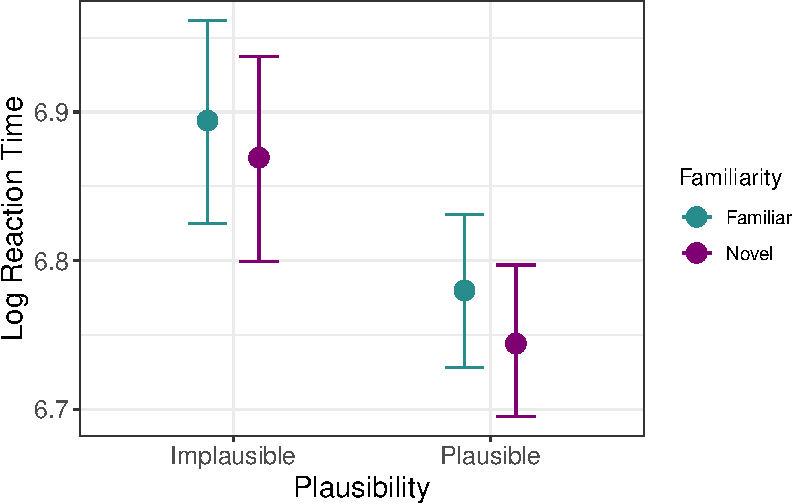
\includegraphics[width=0.8\linewidth,height=\textheight,keepaspectratio]{Chapters/Compound Nouns/staub_rep_ext_files/figure-pdf/fig-N1Staub-1.pdf}

}

\end{figure}%

\begin{figure}[htbp]

\caption{\label{fig-N2Staub}Plot of log reaction time at the N2 region
as a function of plausibility and familiarity.}

\centering{

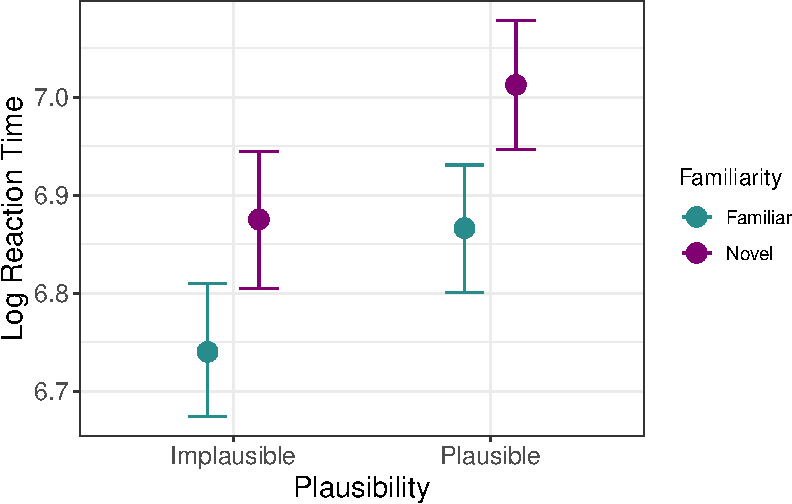
\includegraphics[width=0.8\linewidth,height=\textheight,keepaspectratio]{Chapters/Compound Nouns/staub_rep_ext_files/figure-pdf/fig-N2Staub-1.pdf}

}

\end{figure}%

\subsection{Discussion}\label{discussion}

Our results directly replicate Staub et al.
(\citeproc{ref-staubTimeCoursePlausibility2007}{2007}) using the Maze
task, demonstrating the viability of this method for the tasks at hand.
For the N1 region, while there was a clear increase in reaction time for
items in the implausible condition, there was no interaction effect
between plausibility and familiarity. In other words, the effect of
plausibility was the same for both familiar and novel compound nouns. If
familiar compound nouns are stored holistically, however, it is possible
that we would see less of a (im)plausibility effect relative to novel
items, because readers might be predicting the second noun in the
compound upon reading the first noun. Recall the earlier example,
reproduced below for convenience:

\begin{exe}
\ex Local Plausible and Local Implausible Sentences
\begin{xlist}
\ex Novel Compound
\begin{xlist}
\ex The zookeeper picked up the monkey medicine that was in the enclosure. \hfill \emph{plausible}
\ex The zookeeper spread out the monkey medicine that was in the enclosure. \hfill \emph{implausible}
\end{xlist}
\ex Familiar Compound
\begin{xlist}
\ex Jenny looked out on the huge mountain lion pacing in its cage. \hfill \emph{plausible}
\ex Jenny heard the huge mountain lion pacing in its cage. \hfill \emph{implausible} 
\end{xlist}
\end{xlist}
\end{exe}

\noindent It is possible that if \emph{mountain lion} was stored
holistically, then upon reading \emph{Jenny heard the huge
mountain\ldots{}}, the reader might have less difficulty with the local
implausibility (relative to a low-frequency compound noun) because they
would predict \emph{lion}, which would eliminate the implausibility
(\emph{heard the mountain lion} is not implausible). However, we do not
see this. Instead, the effect of plausibility is similar for both
familiar and novel items. One possible explanation for these results is
that the familiar phrases are not necessarily stored. Instead storage
might be driven by predictability. If this is the case then it would
explain why we do not see this effect in Staub et al.
(\citeproc{ref-staubTimeCoursePlausibility2007}{2007}) or in Experiment
1, especially since all of the items used in Staub et al.
(\citeproc{ref-staubTimeCoursePlausibility2007}{2007}) are
low-predictability compound nouns.

At the N2 region, the decrease in reaction time for familiarity is not
surprising given that familiarity, as previously mentioned, was based on
the frequency of the compound noun as a whole, however the increase in
reaction time for the plausible condition is interesting, especially
since the sentences were only locally implausible on the N1 region: the
second noun in the compound always eliminated the local implausibility.
It is possible this increase in reaction time is a garden path effect
for committing to an interpretation of the sentence with the N1 and
having to reanalyze the sentence. For example, when reading \emph{Jenny
looked upon the huge mountain\ldots{}}, after reading \emph{lion}, the
reader may need to reanalyze the sentence, as the subject is not looking
upon a mountain at all, but rather they are looking at a \emph{mountain
lion}. However, in the implausible condition participants may not fully
commit to the interpretation since it is locally implausible, and thus
may be waiting for a choice that eliminates the implausibility, thus
explaining the absence of a similar slowdown in the implausible
condition.

\section{Experiment 2}\label{experiment-2}

Experiment 1 demonstrated that readers are slower to read the first noun
in a compound noun that is in a locally implausible context, regardless
of the frequency of the compound noun. In Experiment 2, we examine
whether readers can overcome this slowdown due to the local
implausibility if the compound noun is a high-predictability compound
noun.

\subsection{Methods}\label{methods-1}

\subsubsection{Participants}\label{participants-1}

Participant recruitment was identical to Experiment 1. 105 participants
were recruited, and 19 participants were excluded for being below 70\%
accuracy, leaving a total of 86 participants. All participants
self-reported being native English speakers.

\subsubsection{Stimuli}\label{stimuli-1}

We operationalized predictability through the odds ratio of the compound
noun to the first word when that word is not followed by the second word
in the compound noun which is exemplified in
Equation~\ref{eq-oddsratio}.

\begin{equation}\phantomsection\label{eq-oddsratio}{
\frac{\mathrm{count(\textit{peanut butter})}}{\mathrm{count(\textit{peanut})} - \mathrm{count(\textit{peanut butter})}} 
}\end{equation}

In non-mathematical terms, Equation~\ref{eq-oddsratio} quantifies how
predictable the first noun is of the second noun (i.e., how likely the
second noun is to follow after the first noun, relative to every other
word that could follow). For example, the odds ratio of \emph{peanut
butter} would be the odds ratio of the compound noun -- \emph{peanut
butter} -- to the first noun -- \emph{peanut} -- when \emph{butter} does
not follow it.

In order to collect the most predictable compound nouns, we searched the
Google \emph{n}-grams corpus
(\citeproc{ref-michel2011quantitativeanalysisculture}{Michel et al.,
2011}) using the ZS Python package
(\citeproc{ref-smithZSFileFormat2014}{Smith, 2014}). We then collected
the compound nouns with the highest predictability values, using the
following exclusion criteria: excluding words with a match count below
90,000,\footnote{This was done in order to help filter out nonsense
  words (e.g., \emph{teawhit head}) as well as eliminate words that had
  high predictability scores but were just a product of the corpus and
  unlikely to reflect the input of human learners (e.g.,
  \emph{broomwheat tea} which has a predictability score of 287 in the
  corpus).} excluding nonsense words, proper nouns, technical words
(e.g., \emph{tenth circuit}), and words in which we could not create
locally plausible and implausible sentences.\footnote{Given our
  methodology, we needed to be able to make sentences that were
  plausible and implausible using the same compound noun. This
  restriction meant we had to exclude words like \emph{Parmesan cheese}
  where it would be impossible for the reading at the N1 region to be
  implausible without the reading of the compound noun also being
  implausible.} We gathered a total of 37 compound nouns for our
high-predictability condition.

We subsequently normed the sentences we created using the
high-predictability compounds, as well as the sentences from Staub et
al. (\citeproc{ref-staubTimeCoursePlausibility2007}{2007}) which we
confirmed were all low-predictability compounds relative to our compound
nouns.

We followed the same methodology as Staub et al.
(\citeproc{ref-staubTimeCoursePlausibility2007}{2007}) for our norming
procedure: we provided participants with each item in four conditions
(see below) and asked participants to rate each sentence on a 7-point
Likert scale in terms of how well the last word fit in the sentence. No
participant rated more than one version of each sentence. Crucially, for
each item we ensured that sentence 3c received a lower rating than the
other 3 versions of the sentences.

\begin{enumerate} \setcounter{enumi}{2}
   \item \textbf{Norming Conditions}
    \begin{enumerate}
        \item[\textbf{3a}] Jimmy picked up the peanut (plausible, through the first noun).
        \item[\textbf{3b}] Jimmy picked up the peanut butter (plausible, through the second noun).
        \item[\textbf{3c}] Jimmy spread out the peanut (implausible, through the first noun).
        \item[\textbf{3d}] Jimmy spread out the peanut butter (implausible, through the second noun).
    \end{enumerate} \label{figanext}
\end{enumerate}

Finally, we excluded items in which the implausible sentence through the
first noun was rated more or similarly well to the other conditions
(i.e., the plausible sentence through the first noun, the plausible
sentence through the second noun, and the implausible sentence through
the second noun). It is important to note that due to our experimental
design, the implausible sentence through the second noun is technically
plausible at the second noun, because the second noun eliminates the
local implausibility. Thus this condition should also receive a high
rating, despite being the implausible condition. The mean values for
each condition are as follows: plausible, through the first noun: 5.58
(sd = 0.78); plausible, through the second noun: 5.41 (sd = 0.71);
implausible, through the first noun: 3.13 (0.63); implausible, through
the second noun: 5.47 (sd = 0.82).

After norming, we selected sentences such that the difference in
plausibility values between the plausible and implausible conditions
were roughly the same for the high-predictability and low-predictability
conditions. This was done to avoid conflating an interaction effect
between predictability and plausibility with an item-specific effect.
That is, if the plausibility effect was smaller for high-predictability
sentences relative to the low-predictability sentences, then it would be
impossible to tell if the interaction effect between predictability and
plausibility is meaningful or just a product of our stimuli. The mean
plausibility difference for the low-predictability items was 2.47 and
the mean plausibility difference for the high-predictability items was
2.48. We confirmed that there was not a significant difference in
plausibility values through a t-test (t = 0.0446, df = 39, p = 0.52).
After accounting for this, we ended up with 21 high-predictability and
21 low-predictability items (which were taken from
\citeproc{ref-staubTimeCoursePlausibility2007}{Staub et al., 2007}), for
a total of 42 items. Lastly, in order to avoid participants discerning
the experimental design we also included 188 filler items.

\subsubsection{Procedure}\label{procedure-1}

Following Experiment 1, we used the A-maze task
(\citeproc{ref-boyceMazeMadeEasy2020}{Boyce et al., 2020}) with
automatically-generated distractor items
(\citeproc{ref-gulordava2018colorlessgreenrecurrent}{Gulordava et al.,
2018}). Our dependent variable was reaction time and our independent
variables were plausibility and predictability. We again used ibex farm
to run our maze task. Sentences were presented in a random order and
each word was presented an equal amount of times on the left and right
side of the screen. Additionally, each item appeared an equal number of
times in the implausible and plausible context and no participant was
presented with the same item in more than one condition.

\subsubsection{Analysis}\label{analysis-1}

The data was analyzed using Bayesian linear regression models, as
implemented in the \emph{brms} package
(\citeproc{ref-burknerBrmsPackageBayesian2017}{Bürkner, 2017}) within
the R programming environment (\citeproc{ref-Rpackage}{R Core Team,
2022}). We subsetted the data into two sets based on the region: one set
for the first noun in the compound noun and one set for the second noun
in the compound. The primary dependent variable was log reaction time
for both of these regions (following
\citeproc{ref-boyceMazeMadeEasy2020}{Boyce et al., 2020}). The
independent variables were plausibility and predictability. Reaction
time was modeled as a function of plausibility and predictability, along
with their interaction, with maximal random effects
(\citeproc{ref-barrRandomEffectsStructure2013}{Barr et al., 2013}). The
formula used for the model is presented in Equation~\ref{eq-model2}
below, with \emph{Plaus} as plausibility and \emph{Predic} as
predictability.

\begin{equation}\phantomsection\label{eq-model2}{
Reaction Time\sim Plaus*Predict+(Plaus*Predict|Subject)+(Plaus|Item) 
}\end{equation}

\subsection{Results}\label{results-1}

As mentioned in the methods section, for the purpose of the analysis,
the data was divided into two regions: the N1 region and the N2 region,
which were the first and second noun in the compound noun respectively.
The results of the Bayesian regression models for the N1 region are
presented in Table~\ref{tbl-N1Predictability} and
Table~\ref{tbl-N1LogOdds}, and visualized in
Figure~\ref{fig-N1Predictability} and Figure~\ref{fig-N1LogOdds}. The
results of the N2 region are presented in
Table~\ref{tbl-N2Predictability} and Table~\ref{tbl-N2LogOdds}, and
visualized in Figure~\ref{fig-N2Predictability} and
Figure~\ref{fig-N2LogOdds}.

With regards to the N1 region, Table~\ref{tbl-N1Predictability} presents
the results of the analysis we ran with predictability as a binary
predictor (high or low), while Table~\ref{tbl-N1LogOdds} presents the
results of the analysis we ran with predictability as a continuous
predictor (operationalized as the log odds ratio). Our results
demonstrate that, similar to experiment 1, there was an increase in
reaction time for the implausible condition, but no effect for
predictability or the interaction between the two.

As in Experiment 1, we once again conducted a post-hoc Bayes factor
analysis to compare the interaction effect to the null hypothesis
(interaction effect = 0). We found a Bayes Factor value of 15.67 which
constitutes strong support for the null hypothesis. Specifically, we
used the Save-Dickey density ratio method, which involves comparing two
models: one in which the value of interest is fixed (in this case, the
interaction effect would be fixed at zero) and one in which the value of
interest is free to vary (in this case, the interaction effect would be
allowed to vary). The Bayes factor is then obtained by dividing the
height of the posterior for the parameter under the model that allows
the interaction effect to vary by the height of the prior for that
parameter
(\citeproc{ref-wagenmakers2010bayesianhypothesistesting}{Wagenmakers et
al., 2010}).\footnote{The code to reproduce the Bayes factor is included
  at the following link:
  \url{https://github.com/znhoughton/dissertation_writeup/blob/master/Chapters/Compound\%20Nouns/Analysis\%20Scripts/data_analysis.qmd}.}
We computed the Bayes factor for the N1 region and not the N2 region
because the interaction at the N2 region is not of particular interest
to our theoretical question.

With regards to the N2 region, Table~\ref{tbl-N2Predictability} presents
the results of the analysis we ran with predictability as a binary
predictor (high or low), while Table~\ref{tbl-N2LogOdds} presents the
results of the analysis we ran with predictability as a continuous
predictor (operationalized as the log odds ratio). Our results, as in
Experiment 1, demonstrate an increase in reaction time in the plausible
condition and and a decrease in reaction time in the high-predictability
condition, but no interaction effect between plausibility and
predictability.

Figure~\ref{fig-N1Predictability} and Figure~\ref{fig-N2Predictability}
provide visualizations of the analyses run with predictability as a
binary variable while Figure~\ref{fig-N1LogOdds} and
Figure~\ref{fig-N2LogOdds} present analyses with predictability as a
continuous variable.

\begin{table}

\caption{\label{tbl-N1Predictability}Regression analysis results for the
N1 region with predictability as a binary predictor (high or low).}

\centering{

\centering\begingroup\fontsize{12}{14}\selectfont

\begin{tabular}{>{\raggedright\arraybackslash}p{12em}rrrrr}
\toprule
\textbf{ } & \textbf{Estimate} & \textbf{Est.Error} & \textbf{Q2.5} & \textbf{Q97.5} & \textbf{\% Samples > 0}\\
\midrule
\textbf{\cellcolor{gray!6}{Intercept}} & \cellcolor{gray!6}{6.88} & \cellcolor{gray!6}{0.03} & \cellcolor{gray!6}{6.82} & \cellcolor{gray!6}{6.94} & \cellcolor{gray!6}{100.00}\\
\textbf{Plausibility} & 0.07 & 0.01 & 0.04 & 0.10 & 100.00\\
\textbf{\cellcolor{gray!6}{Predictability}} & \cellcolor{gray!6}{0.03} & \cellcolor{gray!6}{0.02} & \cellcolor{gray!6}{-0.01} & \cellcolor{gray!6}{0.08} & \cellcolor{gray!6}{92.30}\\
\textbf{Plausibility:Predictability} & 0.00 & 0.01 & -0.03 & 0.03 & 46.72\\
\bottomrule
\end{tabular}
\endgroup{}

}

\end{table}%

\begin{table}

\caption{\label{tbl-N1LogOdds}Regression analysis results for the N1
region with predictability as a continuous predictor (log odds ratio).}

\centering{

\centering\begingroup\fontsize{12}{14}\selectfont

\begin{tabular}{>{\raggedright\arraybackslash}p{12em}rrrrr}
\toprule
\textbf{ } & \textbf{Estimate} & \textbf{Est.Error} & \textbf{Q2.5} & \textbf{Q97.5} & \textbf{\% Samples > 0}\\
\midrule
\textbf{\cellcolor{gray!6}{Intercept}} & \cellcolor{gray!6}{6.88} & \cellcolor{gray!6}{0.03} & \cellcolor{gray!6}{6.82} & \cellcolor{gray!6}{6.93} & \cellcolor{gray!6}{100.00}\\
\textbf{Plausibility} & 0.07 & 0.01 & 0.04 & 0.10 & 100.00\\
\textbf{\cellcolor{gray!6}{LogOdds}} & \cellcolor{gray!6}{0.00} & \cellcolor{gray!6}{0.01} & \cellcolor{gray!6}{-0.01} & \cellcolor{gray!6}{0.02} & \cellcolor{gray!6}{76.50}\\
\textbf{Plausibility:LogOdds} & 0.00 & 0.00 & -0.01 & 0.01 & 61.64\\
\bottomrule
\end{tabular}
\endgroup{}

}

\end{table}%

\begin{table}

\caption{\label{tbl-N2Predictability}Regression analysis results for the
N2 region with predictability as a binary predictor (high or low).}

\centering{

\centering\begingroup\fontsize{12}{14}\selectfont

\begin{tabular}{>{\raggedright\arraybackslash}p{12em}rrrrr}
\toprule
\textbf{ } & \textbf{Estimate} & \textbf{Est.Error} & \textbf{Q2.5} & \textbf{Q97.5} & \textbf{\% Samples > 0}\\
\midrule
\textbf{\cellcolor{gray!6}{Intercept}} & \cellcolor{gray!6}{6.79} & \cellcolor{gray!6}{0.03} & \cellcolor{gray!6}{6.74} & \cellcolor{gray!6}{6.85} & \cellcolor{gray!6}{100.00}\\
\textbf{Plausibility} & -0.07 & 0.01 & -0.10 & -0.05 & 0.00\\
\textbf{\cellcolor{gray!6}{Predictability}} & \cellcolor{gray!6}{-0.08} & \cellcolor{gray!6}{0.03} & \cellcolor{gray!6}{-0.13} & \cellcolor{gray!6}{-0.03} & \cellcolor{gray!6}{0.12}\\
\textbf{Plausibility:Predictability} & 0.00 & 0.01 & -0.02 & 0.03 & 67.46\\
\bottomrule
\end{tabular}
\endgroup{}

}

\end{table}%

\begin{table}

\caption{\label{tbl-N2LogOdds}Regression analysis results for the N2
region with predictability as a continuous predictor (log odds ratio).}

\centering{

\centering\begingroup\fontsize{12}{14}\selectfont

\begin{tabular}{>{\raggedright\arraybackslash}p{12em}rrrrr}
\toprule
\textbf{ } & \textbf{Estimate} & \textbf{Est.Error} & \textbf{Q2.5} & \textbf{Q97.5} & \textbf{\% Samples > 0}\\
\midrule
\textbf{\cellcolor{gray!6}{Intercept}} & \cellcolor{gray!6}{6.80} & \cellcolor{gray!6}{0.03} & \cellcolor{gray!6}{6.75} & \cellcolor{gray!6}{6.85} & \cellcolor{gray!6}{100.00}\\
\textbf{Plausibility} & -0.07 & 0.01 & -0.10 & -0.05 & 0.00\\
\textbf{\cellcolor{gray!6}{LogOdds}} & \cellcolor{gray!6}{-0.03} & \cellcolor{gray!6}{0.01} & \cellcolor{gray!6}{-0.05} & \cellcolor{gray!6}{-0.02} & \cellcolor{gray!6}{0.00}\\
\textbf{Plausibility:LogOdds} & 0.00 & 0.00 & -0.01 & 0.01 & 60.44\\
\bottomrule
\end{tabular}
\endgroup{}

}

\end{table}%

\begin{figure}[htbp]

\caption{\label{fig-N1Predictability}Plot of the N1 region with
predictability as a binary variable (high or low).}

\centering{

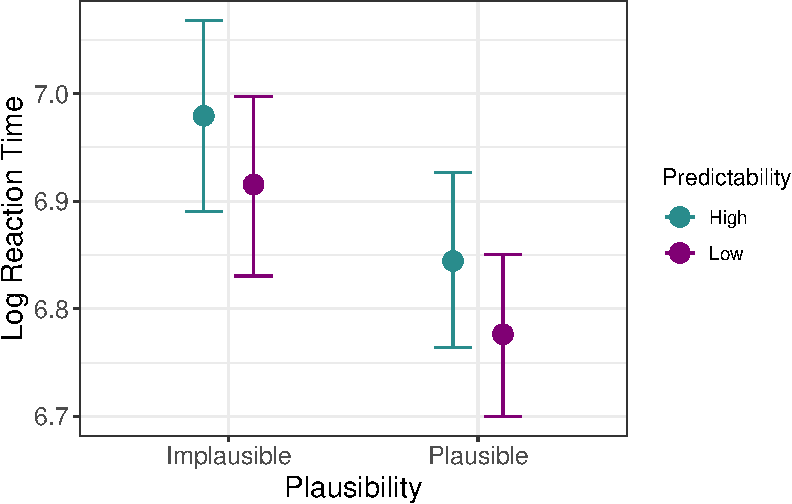
\includegraphics[width=0.8\linewidth,height=\textheight,keepaspectratio]{Chapters/Compound Nouns/staub_rep_ext_files/figure-pdf/fig-N1Predictability-1.pdf}

}

\end{figure}%

\begin{figure}[htbp]

\caption{\label{fig-N1LogOdds}Plot of the N1 region with predictability
as a continuous variable.}

\centering{

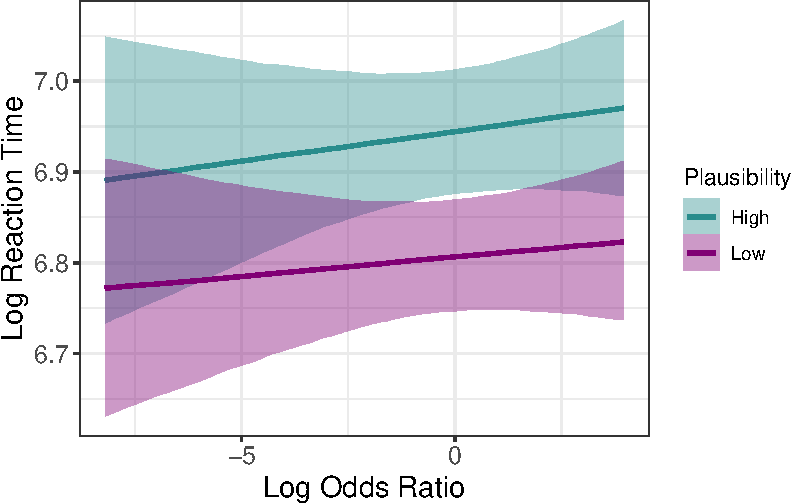
\includegraphics[width=0.8\linewidth,height=\textheight,keepaspectratio]{Chapters/Compound Nouns/staub_rep_ext_files/figure-pdf/fig-N1LogOdds-1.pdf}

}

\end{figure}%

\begin{figure}[htbp]

\caption{\label{fig-N2Predictability}Plot of the N2 region with
predictability as a binary variable (high or low).}

\centering{

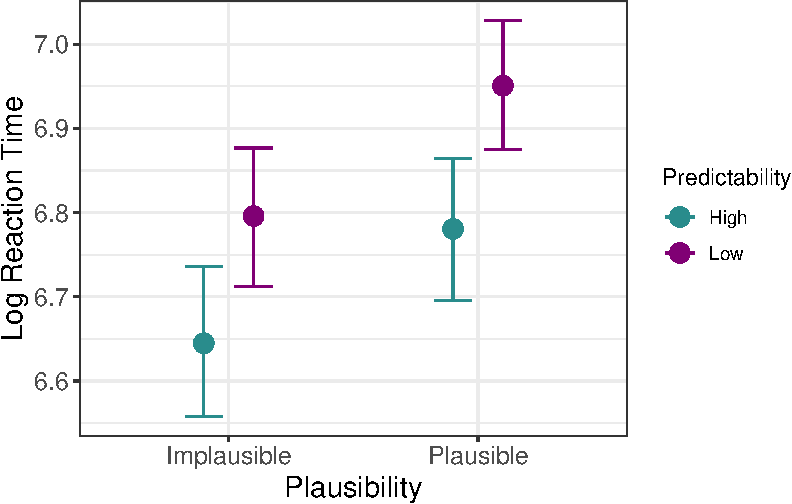
\includegraphics[width=0.8\linewidth,height=\textheight,keepaspectratio]{Chapters/Compound Nouns/staub_rep_ext_files/figure-pdf/fig-N2Predictability-1.pdf}

}

\end{figure}%

\begin{figure}[htbp]

\caption{\label{fig-N2LogOdds}Plot of the N2 region with predictability
as a continuous variable.}

\centering{

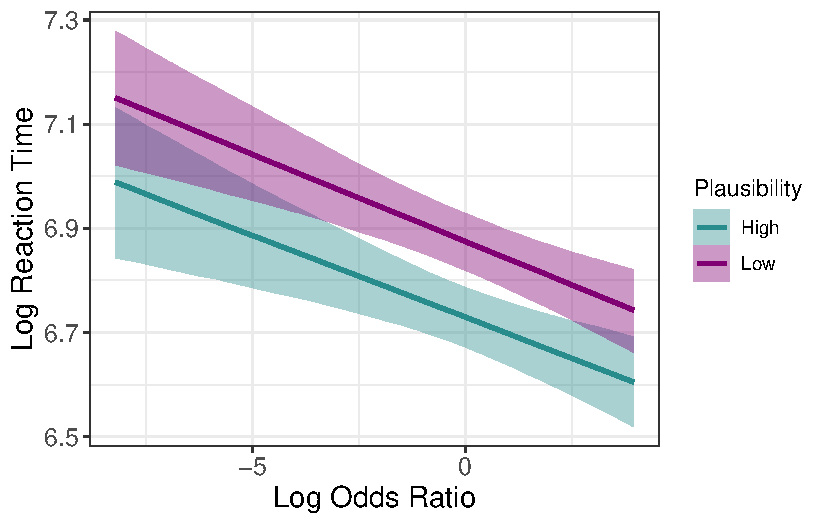
\includegraphics[width=0.8\linewidth,height=\textheight,keepaspectratio]{Chapters/Compound Nouns/staub_rep_ext_files/figure-pdf/fig-N2LogOdds-1.pdf}

}

\end{figure}%

\subsection{Discussion}\label{discussion-1}

Experiment 2 replicates and extends Experiment 1 using predictability
instead of familiarity (i.e., phrasal frequency). Interestingly, the
results of Experiment 2 were extremely similar to the results of
Experiment 1: There was no interaction effect between predictability and
plausibility on the RTs for the N1 condition. Additionally, while we see
an effect of implausibility on the N1 region, we don't see an effect of
predictability. This is expected since predictability is defined as the
odds that the N2 appears given the N1, so we should see this effect on
the N2 region, not the N1 region.

The results of the N2 region also bear remarkable similarities to our
results in Experiment 1: There was a plausibility and predictability
effect, but no interaction between the two. Specifically, there was an
\emph{increase} in reaction time for items in the plausible condition
relative to the implausible condition. It is possible that, as mentioned
in the discussion section of Experiment 1, this increase in reaction
time is a garden path effect for committing to an interpretation of the
sentence with the N1 and having to reanalyze the sentence.

\section{Experiment 3}\label{experiment-3}

In Experiments 1 and 2, we demonstrated that there is a slowdown at the
N1 region in locally implausible contexts. However, the maze task
requires participants to actively decide on the continuation of the
sentence (by selecting the correct word). This may encourage a more
readers to commit to an interpretation more than they would in a more
naturalistic reading task. Thus, in Experiment 3, we directly replicate
Experiment 1 using eye-tracking. We use the same Experimental items and
Filler items as in Experiment 1, however we also included comprehension
questions to check participants' attention.

\subsection{Methods}\label{methods-2}

\subsubsection{Participants}\label{participants-2}

46 native English speakers were recruited from the University of
California, Davis subjects pool. They were given course credit in
exchange for their participation. All participants had normal or
corrected vision.

\subsubsection{Materials}\label{materials}

The materials were identical to Experiment 1, however they also included
comprehension questions.

We recorded participants' right pupil movements using the Eyelink 1000
Plus. Participants were seated 850mm away from the screen, which was
531.3mm in width, 298.8mm in height, and had a resolution of 1920x1080.

Comprehension was checked for non-experimental trials and participants
below 80\% accuracy were excluded. Out of our 46 participants, 2 were
excluded for falling below the accuracy threshold.

\subsubsection{Analyses}\label{analyses}

Prior to our analyses, sentences with blinks were excluded and fixations
less than 80ms in duration and within one character of the nearest
fixation were merged into that fixation (following
\citeproc{ref-staubTimeCoursePlausibility2007}{Staub et al., 2007}). For
our regions of interest (the first noun and the second noun in the
compound noun), we computed first fixation duration, first pass time,
go-past time, and first-pass regression.

For each analysis, our independent variables were plausibility (high or
low) and familiarity (high or low) and their interaction. We also
included random slopes for condition and predictability by subject and
plausibility by compound noun as well as intercepts for subject and
compound noun. For each of our models, we used sum-coding, where the
intercept represents the grand mean and the fixed-effect coefficient
estimates represent the distance from the grand mean.

\subsection{Results}\label{results-2}

\subsubsection{N1 Region}\label{n1-region}

Our results at the N1 region are demonstrated in
Table~\ref{tbl-fullmodelresultsn1staub} and visualized in
Figure~\ref{fig-fullmodelresultsn1staub}.

At the N1 region, we find main-effects of plausibility for first
fixation duration, go-past time, and first-pass regression, but not for
gaze times. Additionally, we find no effects of familiarity. Finally,
for go-past times we find an interaction between plausibility and
predictability such that the slowdown of the implausible context was
greater for familiar items than novel items.

\begin{table}

\caption{\label{tbl-fullmodelresultsn1staub}Model results for each
eye-tracking measure at the N1 region.}

\centering{

\centering\begingroup\fontsize{12}{14}\selectfont

\begin{tabular}{>{\raggedright\arraybackslash}p{12em}rrrrr}
\toprule
\textbf{ } & \textbf{Estimate} & \textbf{Est.Error} & \textbf{Q2.5} & \textbf{Q97.5} & \textbf{\% Samples > 0}\\
\midrule
\addlinespace[0.3em]
\multicolumn{6}{l}{\textbf{First Fixation Duration}}\\
\textbf{\hspace{1em}\cellcolor{gray!6}{Intercept}} & \cellcolor{gray!6}{239.23} & \cellcolor{gray!6}{5.54} & \cellcolor{gray!6}{228.46} & \cellcolor{gray!6}{250.05} & \cellcolor{gray!6}{100.00}\\
\textbf{\hspace{1em}Plausibility} & 4.19 & 2.16 & -0.02 & 8.38 & 97.40\\
\textbf{\hspace{1em}\cellcolor{gray!6}{Familiarity}} & \cellcolor{gray!6}{-0.87} & \cellcolor{gray!6}{2.40} & \cellcolor{gray!6}{-5.59} & \cellcolor{gray!6}{3.78} & \cellcolor{gray!6}{35.52}\\
\textbf{\hspace{1em}Plausibility:Familiarity} & 0.03 & 2.40 & -4.84 & 4.78 & 49.68\\
\addlinespace[0.3em]
\multicolumn{6}{l}{\textbf{Gaze/First-Pass Duration}}\\
\textbf{\hspace{1em}\cellcolor{gray!6}{Intercept}} & \cellcolor{gray!6}{273.96} & \cellcolor{gray!6}{8.56} & \cellcolor{gray!6}{257.09} & \cellcolor{gray!6}{290.93} & \cellcolor{gray!6}{100.00}\\
\textbf{\hspace{1em}Plausibility} & 0.04 & 0.20 & -0.33 & 0.42 & 57.83\\
\textbf{\hspace{1em}\cellcolor{gray!6}{Familiarity}} & \cellcolor{gray!6}{0.00} & \cellcolor{gray!6}{0.20} & \cellcolor{gray!6}{-0.40} & \cellcolor{gray!6}{0.38} & \cellcolor{gray!6}{49.73}\\
\textbf{\hspace{1em}Plausibility:Familiarity} & 0.01 & 0.20 & -0.38 & 0.40 & 51.92\\
\addlinespace[0.3em]
\multicolumn{6}{l}{\textbf{Go-Past Time}}\\
\textbf{\hspace{1em}\cellcolor{gray!6}{Intercept}} & \cellcolor{gray!6}{363.00} & \cellcolor{gray!6}{18.58} & \cellcolor{gray!6}{325.95} & \cellcolor{gray!6}{399.74} & \cellcolor{gray!6}{100.00}\\
\textbf{\hspace{1em}Plausibility} & 16.90 & 6.91 & 3.61 & 30.54 & 99.37\\
\textbf{\hspace{1em}\cellcolor{gray!6}{Familiarity}} & \cellcolor{gray!6}{-3.75} & \cellcolor{gray!6}{7.89} & \cellcolor{gray!6}{-19.44} & \cellcolor{gray!6}{11.85} & \cellcolor{gray!6}{31.34}\\
\textbf{\hspace{1em}Plausibility:Familiarity} & 14.84 & 7.42 & 0.45 & 29.41 & 97.77\\
\addlinespace[0.3em]
\multicolumn{6}{l}{\textbf{First-Pass Regression}}\\
\textbf{\hspace{1em}\cellcolor{gray!6}{Intercept}} & \cellcolor{gray!6}{-1.99} & \cellcolor{gray!6}{0.18} & \cellcolor{gray!6}{-2.35} & \cellcolor{gray!6}{-1.64} & \cellcolor{gray!6}{0.00}\\
\textbf{\hspace{1em}Plausibility} & 0.16 & 0.09 & -0.01 & 0.33 & 96.38\\
\textbf{\hspace{1em}\cellcolor{gray!6}{Familiarity}} & \cellcolor{gray!6}{0.02} & \cellcolor{gray!6}{0.09} & \cellcolor{gray!6}{-0.15} & \cellcolor{gray!6}{0.19} & \cellcolor{gray!6}{57.80}\\
\textbf{\hspace{1em}Plausibility:Familiarity} & 0.06 & 0.09 & -0.12 & 0.23 & 74.50\\
\bottomrule
\end{tabular}
\endgroup{}

}

\end{table}%

\begin{figure}[htbp]

\caption{\label{fig-fullmodelresultsn1staub}Visualization of the effects
of plausibility and familiarity on each eye-tracking measure at the N1
region.}

\centering{

\pandocbounded{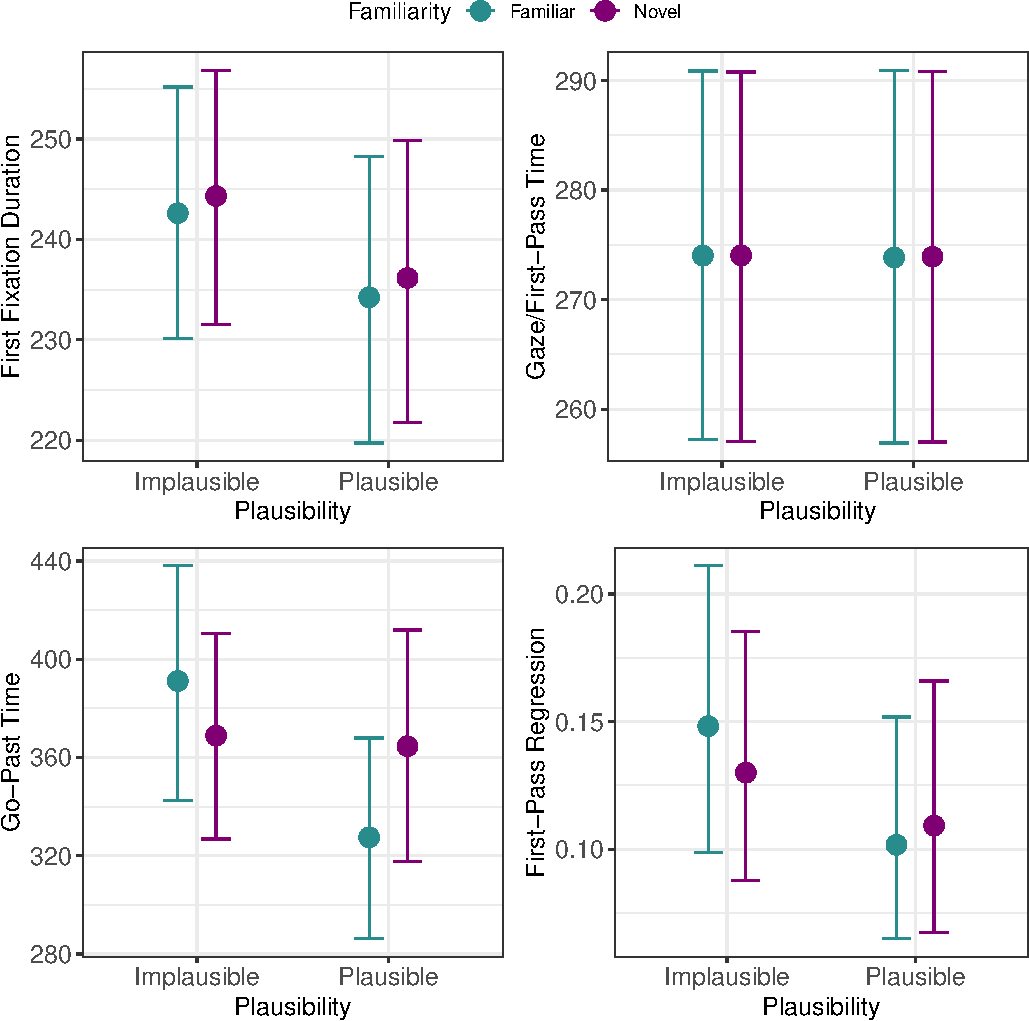
\includegraphics[keepaspectratio]{Chapters/Compound Nouns/staub_rep_ext_files/figure-pdf/fig-fullmodelresultsn1staub-1.pdf}}

}

\end{figure}%

\subsubsection{N2 Region}\label{n2-region}

Our results at the N2 region are demonstrated in
Table~\ref{tbl-fullmodelresultsn2staub} and visualized in
Figure~\ref{fig-fullmodelresultsn2staub}.

At the N2 region, we find main-effects of familiarity for first fixation
duration and gaze times, and marginal effects for go-past times and
first-pass regression. We find no main-effect of plausibility, which is
expected because the implausible condition is plausible at the N2
region. We also find no interaction effect between plausibility and
familiarity.

\begin{table}

\caption{\label{tbl-fullmodelresultsn2staub}Results of models for each
eye-tracking measure at the N2 region.}

\centering{

\centering\begingroup\fontsize{12}{14}\selectfont

\begin{tabular}{>{\raggedright\arraybackslash}p{12em}rrrrr}
\toprule
\textbf{ } & \textbf{Estimate} & \textbf{Est.Error} & \textbf{Q2.5} & \textbf{Q97.5} & \textbf{\% Samples > 0}\\
\midrule
\addlinespace[0.3em]
\multicolumn{6}{l}{\textbf{First Fixation Duration}}\\
\textbf{\hspace{1em}\cellcolor{gray!6}{Intercept}} & \cellcolor{gray!6}{249.62} & \cellcolor{gray!6}{6.47} & \cellcolor{gray!6}{236.38} & \cellcolor{gray!6}{262.35} & \cellcolor{gray!6}{100.00}\\
\textbf{\hspace{1em}Plausibility} & -2.09 & 2.65 & -7.40 & 3.12 & 21.58\\
\textbf{\hspace{1em}\cellcolor{gray!6}{Familiarity}} & \cellcolor{gray!6}{-6.97} & \cellcolor{gray!6}{4.27} & \cellcolor{gray!6}{-15.43} & \cellcolor{gray!6}{1.44} & \cellcolor{gray!6}{5.42}\\
\textbf{\hspace{1em}Plausibility:Familiarity} & -1.05 & 2.37 & -5.67 & 3.62 & 32.48\\
\addlinespace[0.3em]
\multicolumn{6}{l}{\textbf{Gaze/First-Pass Duration}}\\
\textbf{\hspace{1em}\cellcolor{gray!6}{Intercept}} & \cellcolor{gray!6}{275.48} & \cellcolor{gray!6}{9.04} & \cellcolor{gray!6}{257.70} & \cellcolor{gray!6}{293.10} & \cellcolor{gray!6}{100.00}\\
\textbf{\hspace{1em}Plausibility} & 0.05 & 3.76 & -7.50 & 7.44 & 50.55\\
\textbf{\hspace{1em}\cellcolor{gray!6}{Familiarity}} & \cellcolor{gray!6}{-12.96} & \cellcolor{gray!6}{6.37} & \cellcolor{gray!6}{-24.98} & \cellcolor{gray!6}{-0.20} & \cellcolor{gray!6}{2.33}\\
\textbf{\hspace{1em}Plausibility:Familiarity} & -3.88 & 3.78 & -11.31 & 3.42 & 15.24\\
\addlinespace[0.3em]
\multicolumn{6}{l}{\textbf{Go-Past Time}}\\
\textbf{\hspace{1em}\cellcolor{gray!6}{Intercept}} & \cellcolor{gray!6}{351.82} & \cellcolor{gray!6}{21.88} & \cellcolor{gray!6}{308.49} & \cellcolor{gray!6}{394.20} & \cellcolor{gray!6}{100.00}\\
\textbf{\hspace{1em}Plausibility} & 6.95 & 8.40 & -9.27 & 23.77 & 79.87\\
\textbf{\hspace{1em}\cellcolor{gray!6}{Familiarity}} & \cellcolor{gray!6}{-17.43} & \cellcolor{gray!6}{13.36} & \cellcolor{gray!6}{-44.88} & \cellcolor{gray!6}{7.49} & \cellcolor{gray!6}{8.97}\\
\textbf{\hspace{1em}Plausibility:Familiarity} & -7.96 & 9.35 & -26.62 & 10.25 & 19.43\\
\addlinespace[0.3em]
\multicolumn{6}{l}{\textbf{First-Pass Regression}}\\
\textbf{\hspace{1em}\cellcolor{gray!6}{Intercept}} & \cellcolor{gray!6}{-2.31} & \cellcolor{gray!6}{0.21} & \cellcolor{gray!6}{-2.75} & \cellcolor{gray!6}{-1.91} & \cellcolor{gray!6}{0.00}\\
\textbf{\hspace{1em}Plausibility} & 0.07 & 0.09 & -0.10 & 0.26 & 78.45\\
\textbf{\hspace{1em}\cellcolor{gray!6}{Familiarity}} & \cellcolor{gray!6}{-0.14} & \cellcolor{gray!6}{0.12} & \cellcolor{gray!6}{-0.37} & \cellcolor{gray!6}{0.10} & \cellcolor{gray!6}{11.58}\\
\textbf{\hspace{1em}Plausibility:Familiarity} & 0.00 & 0.09 & -0.18 & 0.17 & 48.58\\
\bottomrule
\end{tabular}
\endgroup{}

}

\end{table}%

\begin{figure}[htbp]

\caption{\label{fig-fullmodelresultsn2staub}Visualization of the effects
of plausibility and familiarity on each eye-tracking measure at the N2
region.}

\centering{

\pandocbounded{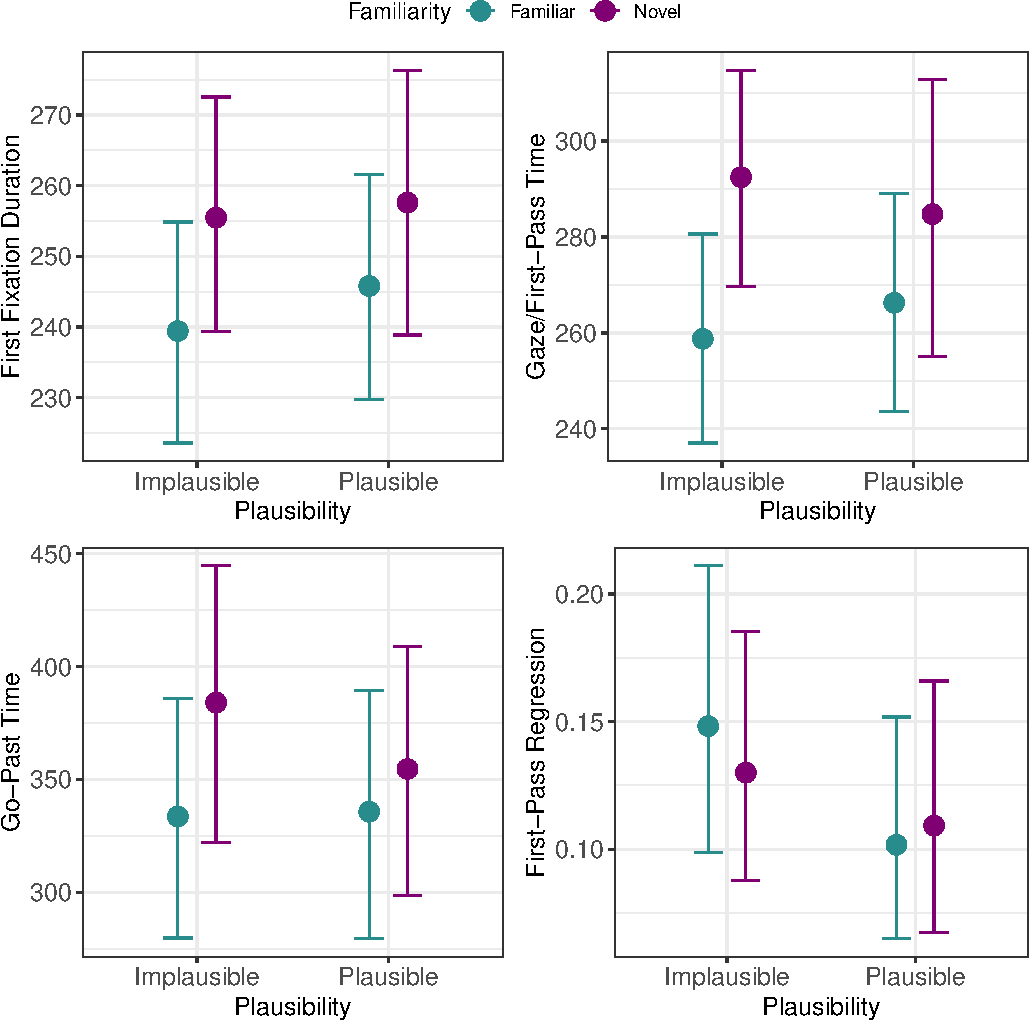
\includegraphics[keepaspectratio]{Chapters/Compound Nouns/staub_rep_ext_files/figure-pdf/fig-fullmodelresultsn2staub-1.pdf}}

}

\end{figure}%

\subsection{Discussion}\label{discussion-2}

Experiment 3 demonstrates that readers have longer first-fixation times,
longer go-past times, and more first-pass regressions in implausible
contexts than in plausible contexts. Further, we find an interaction
effect in the opposite direction from predicted for go-past times: the
effect of plausibility is greater for familiar items than in novel
items. This suggests that the slowdown generated by the locally
implausible context is even greater for familiar items than novel items.
However, since we only find this in one eye-tracking measure, it is
unclear whether this effect is robust or not.

The results of Experiment 3 replicate the results found in both
Experiment 1 and Staub et al.
(\citeproc{ref-staubTimeCoursePlausibility2007}{2007}). That is, in
general, readers take longer to process the first noun in the locally
implausible condition. Further, the frequency of the compound noun does
not alleviate this increase in processing time. In other words, even in
cases where the compound noun is frequent, the implausible context
causes an increase in processing time equal in magnitude to lower
frequency compound nouns. We do find an interaction effect in the
opposite direction as predicted, however since we find it in only one
eye-tracking measure, it is unclear whether it indicates that the local
implausibility is causing readers to have more difficulty processing
frequent compound nouns than infrequent compound nouns.

\section{Experiment 4}\label{experiment-4}

Experiment 3 demonstrated an effect of plausibility at the N1 region
that was consistent regardless of the frequency of the compound noun. In
order to determine whether predictability shows similar effects, in
Experiment 4 we replicate Experiment 2 using eye-tracking. The
Experimental and Filler items were identical, but we also included
comprehension questions to check participants' attention.

\subsection{Methods}\label{methods-3}

\subsubsection{Participants}\label{participants-3}

56 native English speakers were recruited from the University of
California, Davis subjects pool. They were given course credit in
exchange for their participation. All participants had normal or
corrected vision.

\subsubsection{Materials}\label{materials-1}

The materials here were identical to those in Experiment 2, with the
exception of the added comprehension questions.

\subsubsection{Procedure}\label{procedure-2}

We recorded participants' right pupil movements using the Eyelink 1000
Plus. Participants were seated 850mm away from the screen. Our screen
resolution was 1920x1080, 531.3mm in width, and 298.8mm in height.

Comprehension was checked for non-experimental trials and participants
below 80\% accuracy were excluded. Out of our 56 participants, 0 were
excluded for falling below the accuracy threshold.

\subsubsection{Analyses}\label{analyses-1}

Prior to our analyses, sentences with blinks were excluded and fixations
less than 80ms in duration and within one character of the nearest
fixation were merged into that fixation (following
\citeproc{ref-staubTimeCoursePlausibility2007}{Staub et al., 2007}). For
our regions of interest (the first noun and the second noun in the
compound noun), we computed first fixation duration, first pass time,
go-past time, and first-pass regression.

For each analysis, our independent variables were plausibility (high or
low) and (log) predictability (high or low) and their interaction. We
also included random slopes for condition and predictability by subject
and plausibility by compound noun as well as intercepts for subject and
compound noun. For each of our models, we used sum-coding, where the
intercept represents the grand mean and the fixed-effect coefficient
estimates represent the distance from the grand mean.

\subsection{Results}\label{results-3}

\subsubsection{N1 Region}\label{n1-region-1}

Our results at the N1 region are demonstrated in
Table~\ref{tbl-fullmodelresultsn1} and visualized in
Figure~\ref{fig-fullmodelresultsn1}.

At the N1 region, we find main-effects of plausibility for only
first-pass regression. We find no effect of plausibility for first
fixation duration, gaze time, and go-past time. Additionally, we find no
effects of predictability. Finally, we find an interaction effect
between plausibility and predictability for first fixation duration and
first-pass regression. These interaction effects are in the opposite
direction such that the slowdown caused by the implausible condition was
greater for high-predictability items relative to low-predictability
items in first-pass regression, but smaller for high-predictability
items relative to low-predictability items in first fixation duration.

\begin{table}

\caption{\label{tbl-fullmodelresultsn1}Model results for each
eye-tracking measure at the N1 region.}

\centering{

\centering\begingroup\fontsize{12}{14}\selectfont

\begin{tabular}{>{\raggedright\arraybackslash}p{12em}rrrrr}
\toprule
\textbf{ } & \textbf{Estimate} & \textbf{Est.Error} & \textbf{Q2.5} & \textbf{Q97.5} & \textbf{\% Samples > 0}\\
\midrule
\addlinespace[0.3em]
\multicolumn{6}{l}{\textbf{First Fixation Duration}}\\
\textbf{\hspace{1em}\cellcolor{gray!6}{Intercept}} & \cellcolor{gray!6}{231.02} & \cellcolor{gray!6}{4.43} & \cellcolor{gray!6}{222.36} & \cellcolor{gray!6}{239.50} & \cellcolor{gray!6}{100.00}\\
\textbf{\hspace{1em}Plausibility} & 1.66 & 2.02 & -2.29 & 5.70 & 78.95\\
\textbf{\hspace{1em}\cellcolor{gray!6}{Predictability}} & \cellcolor{gray!6}{2.78} & \cellcolor{gray!6}{2.87} & \cellcolor{gray!6}{-2.80} & \cellcolor{gray!6}{8.53} & \cellcolor{gray!6}{83.75}\\
\textbf{\hspace{1em}Plausibility:Predictability} & -3.47 & 2.01 & -7.42 & 0.52 & 4.15\\
\addlinespace[0.3em]
\multicolumn{6}{l}{\textbf{Gaze/First-Pass Duration}}\\
\textbf{\hspace{1em}\cellcolor{gray!6}{Intercept}} & \cellcolor{gray!6}{264.14} & \cellcolor{gray!6}{8.42} & \cellcolor{gray!6}{246.90} & \cellcolor{gray!6}{280.60} & \cellcolor{gray!6}{100.00}\\
\textbf{\hspace{1em}Plausibility} & 0.00 & 0.20 & -0.38 & 0.41 & 49.08\\
\textbf{\hspace{1em}\cellcolor{gray!6}{Predictability}} & \cellcolor{gray!6}{0.00} & \cellcolor{gray!6}{0.20} & \cellcolor{gray!6}{-0.39} & \cellcolor{gray!6}{0.39} & \cellcolor{gray!6}{51.48}\\
\textbf{\hspace{1em}Plausibility:Predictability} & -0.01 & 0.20 & -0.41 & 0.38 & 48.10\\
\addlinespace[0.3em]
\multicolumn{6}{l}{\textbf{Go-Past Time}}\\
\textbf{\hspace{1em}\cellcolor{gray!6}{Intercept}} & \cellcolor{gray!6}{357.21} & \cellcolor{gray!6}{16.45} & \cellcolor{gray!6}{325.20} & \cellcolor{gray!6}{388.96} & \cellcolor{gray!6}{100.00}\\
\textbf{\hspace{1em}Plausibility} & 0.02 & 0.20 & -0.37 & 0.40 & 54.05\\
\textbf{\hspace{1em}\cellcolor{gray!6}{Predictability}} & \cellcolor{gray!6}{0.00} & \cellcolor{gray!6}{0.20} & \cellcolor{gray!6}{-0.39} & \cellcolor{gray!6}{0.39} & \cellcolor{gray!6}{50.10}\\
\textbf{\hspace{1em}Plausibility:Predictability} & 0.00 & 0.20 & -0.39 & 0.39 & 49.77\\
\addlinespace[0.3em]
\multicolumn{6}{l}{\textbf{First-Pass Regression}}\\
\textbf{\hspace{1em}\cellcolor{gray!6}{Intercept}} & \cellcolor{gray!6}{-1.65} & \cellcolor{gray!6}{0.15} & \cellcolor{gray!6}{-1.95} & \cellcolor{gray!6}{-1.36} & \cellcolor{gray!6}{0.00}\\
\textbf{\hspace{1em}Plausibility} & 0.20 & 0.08 & 0.04 & 0.36 & 99.38\\
\textbf{\hspace{1em}\cellcolor{gray!6}{Predictability}} & \cellcolor{gray!6}{-0.05} & \cellcolor{gray!6}{0.09} & \cellcolor{gray!6}{-0.21} & \cellcolor{gray!6}{0.12} & \cellcolor{gray!6}{27.75}\\
\textbf{\hspace{1em}Plausibility:Predictability} & 0.13 & 0.07 & -0.02 & 0.28 & 96.03\\
\bottomrule
\end{tabular}
\endgroup{}

}

\end{table}%

\begin{figure}[htbp]

\caption{\label{fig-fullmodelresultsn1}Visualization of the effects of
plausibility and predictability on each eye-tracking measure at the N1
region.}

\centering{

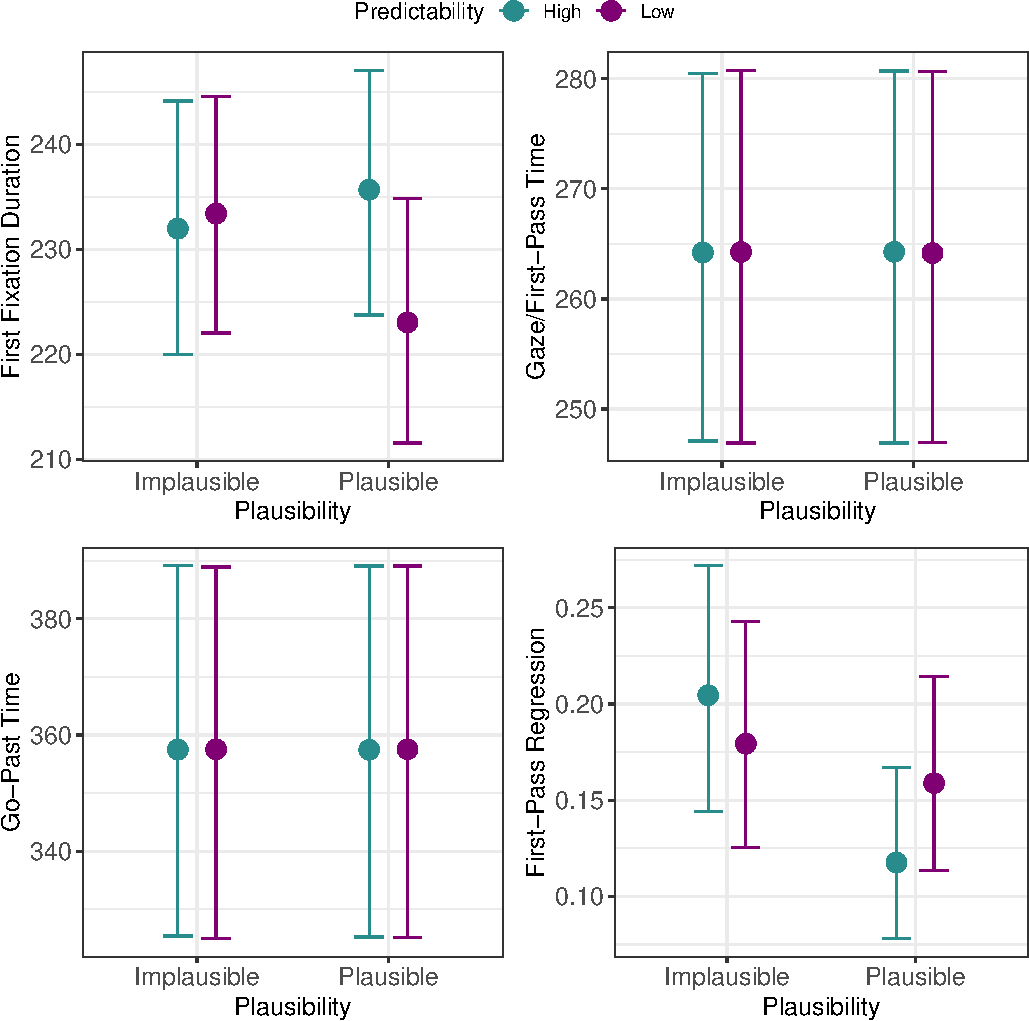
\includegraphics[width=1\linewidth,height=\textheight,keepaspectratio]{Chapters/Compound Nouns/staub_rep_ext_files/figure-pdf/fig-fullmodelresultsn1-1.pdf}

}

\end{figure}%

\subsubsection{N2 Region}\label{n2-region-1}

Our results at the N2 region are demonstrated in
Table~\ref{tbl-fullmodelresultsn2} and visualized in
Figure~\ref{fig-fullmodelresultsn2}.

At the N2 region, we find a main-effect of predictability for only the
first fixation duration measure. We find no effect of plausibility, as
expected because the N2 region eliminates the implausibility effect. We
also find no interaction between plausibility and predictability in any
of the measures.

\begin{table}

\caption{\label{tbl-fullmodelresultsn2}Model results for each
eye-tracking measure at the N2 region.}

\centering{

\centering\begingroup\fontsize{12}{14}\selectfont

\begin{tabular}{>{\raggedright\arraybackslash}p{12em}rrrrr}
\toprule
\textbf{ } & \textbf{Estimate} & \textbf{Est.Error} & \textbf{Q2.5} & \textbf{Q97.5} & \textbf{\% Samples > 0}\\
\midrule
\addlinespace[0.3em]
\multicolumn{6}{l}{\textbf{First Fixation Duration}}\\
\textbf{\hspace{1em}\cellcolor{gray!6}{Intercept}} & \cellcolor{gray!6}{234.45} & \cellcolor{gray!6}{4.86} & \cellcolor{gray!6}{224.48} & \cellcolor{gray!6}{243.77} & \cellcolor{gray!6}{100.00}\\
\textbf{\hspace{1em}Plausibility} & -2.15 & 2.97 & -8.13 & 3.68 & 23.23\\
\textbf{\hspace{1em}\cellcolor{gray!6}{Predictability}} & \cellcolor{gray!6}{-4.14} & \cellcolor{gray!6}{2.99} & \cellcolor{gray!6}{-9.89} & \cellcolor{gray!6}{1.89} & \cellcolor{gray!6}{8.58}\\
\textbf{\hspace{1em}Plausibility:Predictability} & -2.93 & 3.01 & -8.92 & 2.97 & 16.08\\
\addlinespace[0.3em]
\multicolumn{6}{l}{\textbf{Gaze/First-Pass Duration}}\\
\textbf{\hspace{1em}\cellcolor{gray!6}{Intercept}} & \cellcolor{gray!6}{253.76} & \cellcolor{gray!6}{6.07} & \cellcolor{gray!6}{241.73} & \cellcolor{gray!6}{265.77} & \cellcolor{gray!6}{100.00}\\
\textbf{\hspace{1em}Plausibility} & 0.00 & 0.10 & -0.20 & 0.19 & 48.83\\
\textbf{\hspace{1em}\cellcolor{gray!6}{Predictability}} & \cellcolor{gray!6}{0.00} & \cellcolor{gray!6}{0.10} & \cellcolor{gray!6}{-0.21} & \cellcolor{gray!6}{0.19} & \cellcolor{gray!6}{48.62}\\
\textbf{\hspace{1em}Plausibility:Predictability} & 0.00 & 0.10 & -0.20 & 0.20 & 51.62\\
\addlinespace[0.3em]
\multicolumn{6}{l}{\textbf{Go-Past Time}}\\
\textbf{\hspace{1em}\cellcolor{gray!6}{Intercept}} & \cellcolor{gray!6}{342.74} & \cellcolor{gray!6}{12.87} & \cellcolor{gray!6}{317.68} & \cellcolor{gray!6}{367.65} & \cellcolor{gray!6}{100.00}\\
\textbf{\hspace{1em}Plausibility} & 0.00 & 0.10 & -0.20 & 0.20 & 47.60\\
\textbf{\hspace{1em}\cellcolor{gray!6}{Predictability}} & \cellcolor{gray!6}{0.00} & \cellcolor{gray!6}{0.10} & \cellcolor{gray!6}{-0.20} & \cellcolor{gray!6}{0.20} & \cellcolor{gray!6}{50.00}\\
\textbf{\hspace{1em}Plausibility:Predictability} & 0.00 & 0.10 & -0.19 & 0.20 & 49.02\\
\addlinespace[0.3em]
\multicolumn{6}{l}{\textbf{First-Pass Regression}}\\
\textbf{\hspace{1em}\cellcolor{gray!6}{Intercept}} & \cellcolor{gray!6}{-2.06} & \cellcolor{gray!6}{0.18} & \cellcolor{gray!6}{-2.43} & \cellcolor{gray!6}{-1.73} & \cellcolor{gray!6}{0.00}\\
\textbf{\hspace{1em}Plausibility} & -0.03 & 0.11 & -0.24 & 0.18 & 40.62\\
\textbf{\hspace{1em}\cellcolor{gray!6}{Predictability}} & \cellcolor{gray!6}{-0.02} & \cellcolor{gray!6}{0.10} & \cellcolor{gray!6}{-0.22} & \cellcolor{gray!6}{0.18} & \cellcolor{gray!6}{41.10}\\
\textbf{\hspace{1em}Plausibility:Predictability} & 0.05 & 0.10 & -0.14 & 0.24 & 69.97\\
\bottomrule
\end{tabular}
\endgroup{}

}

\end{table}%

\begin{figure}[htbp]

\caption{\label{fig-fullmodelresultsn2}Visualization of the effects of
plausibility and predictability on each eye-tracking measure at the N2
region.}

\centering{

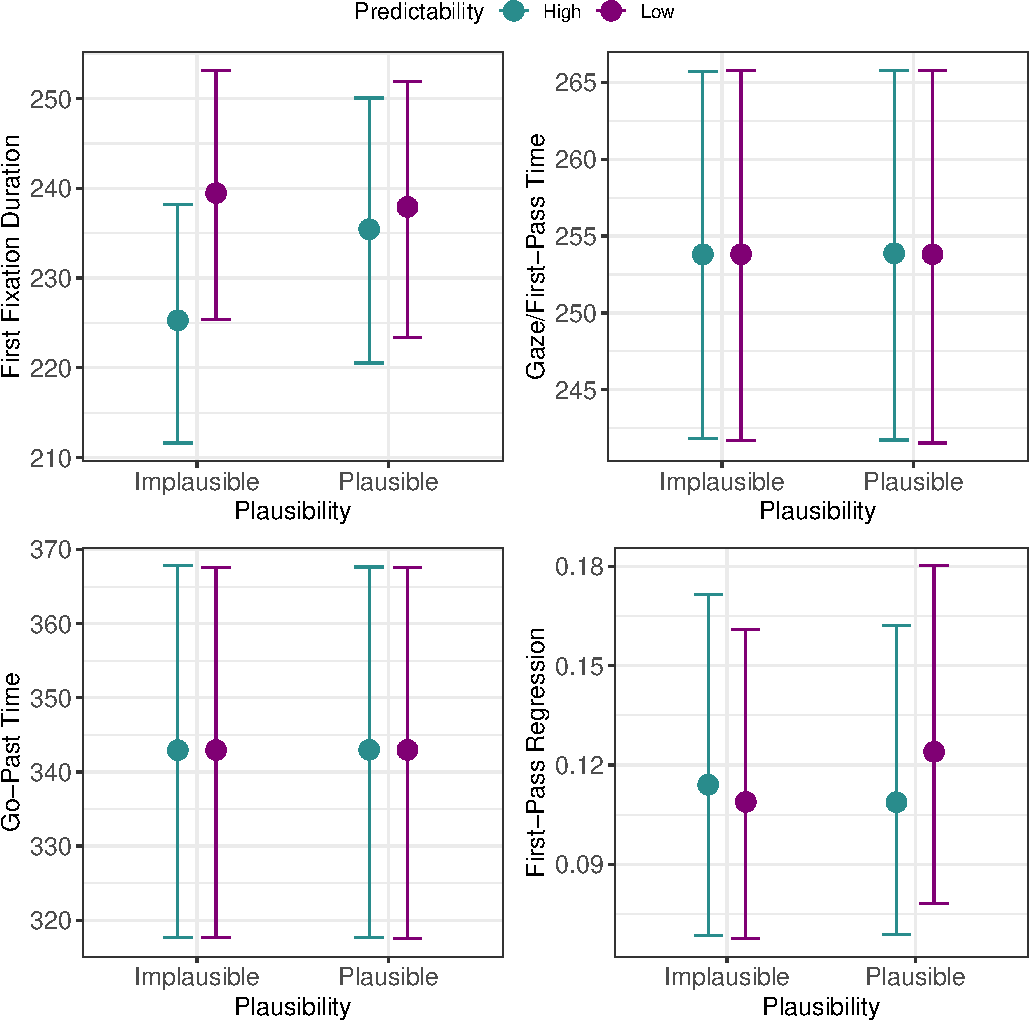
\includegraphics[width=1\linewidth,height=\textheight,keepaspectratio]{Chapters/Compound Nouns/staub_rep_ext_files/figure-pdf/fig-fullmodelresultsn2-1.pdf}

}

\end{figure}%

\subsubsection{Filler Items}\label{filler-items}

In addition to our experimental stimuli, we also included sentences that
varied with respect to the frequency of the word. For example, in the
below sentences, \emph{satchel} is low-frequency and \emph{account} is
high-frequency. Thus, in order to confirm that the results in Experiment
4 were not due to measurement error, we examined the effect of frequency
in our filler items on each of the eye-tracking measures.

\begin{exe}
\ex Filler Sentences \label{fillers}
\begin{xlist}
\ex{Take your money out of the \textbf{satchel} and pay off the debt. \hfill \emph{low-frequency}}
\ex{Take your money out of the \textbf{account} and pay off the debt. \hfill \emph{high-frequency}}
\end{xlist}
\end{exe}

Our results are presented in Table~\ref{tbl-filleritemsall} and
visualized in Figure~\ref{fig-filleritemsall}. We find an effect of
frequency in each of the four eye-tracking measures we looked at.

\begin{table}

\caption{\label{tbl-filleritemsall}Model results for filler items for
each eye-tracking measure.}

\centering{

\centering\begingroup\fontsize{12}{14}\selectfont

\begin{tabular}{>{\raggedright\arraybackslash}p{12em}llllr}
\toprule
\textbf{ } & \textbf{Estimate} & \textbf{Est.Error} & \textbf{Q2.5} & \textbf{Q97.5} & \textbf{\% Samples > 0}\\
\midrule
\addlinespace[0.3em]
\multicolumn{6}{l}{\textbf{First Fixation Duration}}\\
\textbf{\hspace{1em}\cellcolor{gray!6}{Intercept}} & \cellcolor{gray!6}{227.843} & \cellcolor{gray!6}{3.942} & \cellcolor{gray!6}{220.186} & \cellcolor{gray!6}{235.404} & \cellcolor{gray!6}{100.00}\\
\textbf{\hspace{1em}Frequency} & 4.011 & 1.848 & 0.414 & 7.642 & 98.50\\
\addlinespace[0.3em]
\multicolumn{6}{l}{\textbf{Gaze/First-Pass Duration}}\\
\textbf{\hspace{1em}\cellcolor{gray!6}{Intercept}} & \cellcolor{gray!6}{261.710} & \cellcolor{gray!6}{7.805} & \cellcolor{gray!6}{246.338} & \cellcolor{gray!6}{276.992} & \cellcolor{gray!6}{100.00}\\
\textbf{\hspace{1em}Frequency} & 13.825 & 4.371 & 5.179 & 22.322 & 99.88\\
\addlinespace[0.3em]
\multicolumn{6}{l}{\textbf{Go-Past Time}}\\
\textbf{\hspace{1em}\cellcolor{gray!6}{Intercept}} & \cellcolor{gray!6}{368.199} & \cellcolor{gray!6}{17.340} & \cellcolor{gray!6}{334.329} & \cellcolor{gray!6}{402.836} & \cellcolor{gray!6}{100.00}\\
\textbf{\hspace{1em}Frequency} & 24.391 & 7.863 & 9.001 & 39.509 & 99.80\\
\addlinespace[0.3em]
\multicolumn{6}{l}{\textbf{First-Pass Regression}}\\
\textbf{\hspace{1em}\cellcolor{gray!6}{Intercept}} & \cellcolor{gray!6}{-1.659} & \cellcolor{gray!6}{0.129} & \cellcolor{gray!6}{-1.921} & \cellcolor{gray!6}{-1.417} & \cellcolor{gray!6}{0.00}\\
\textbf{\hspace{1em}Frequency} & 0.156 & 0.058 & 0.044 & 0.271 & 99.60\\
\bottomrule
\end{tabular}
\endgroup{}

}

\end{table}%

\begin{figure}[htbp]

\caption{\label{fig-filleritemsall}Visualization of the effects of
frequency on each eye-tracking measure for filler items.}

\centering{

\pandocbounded{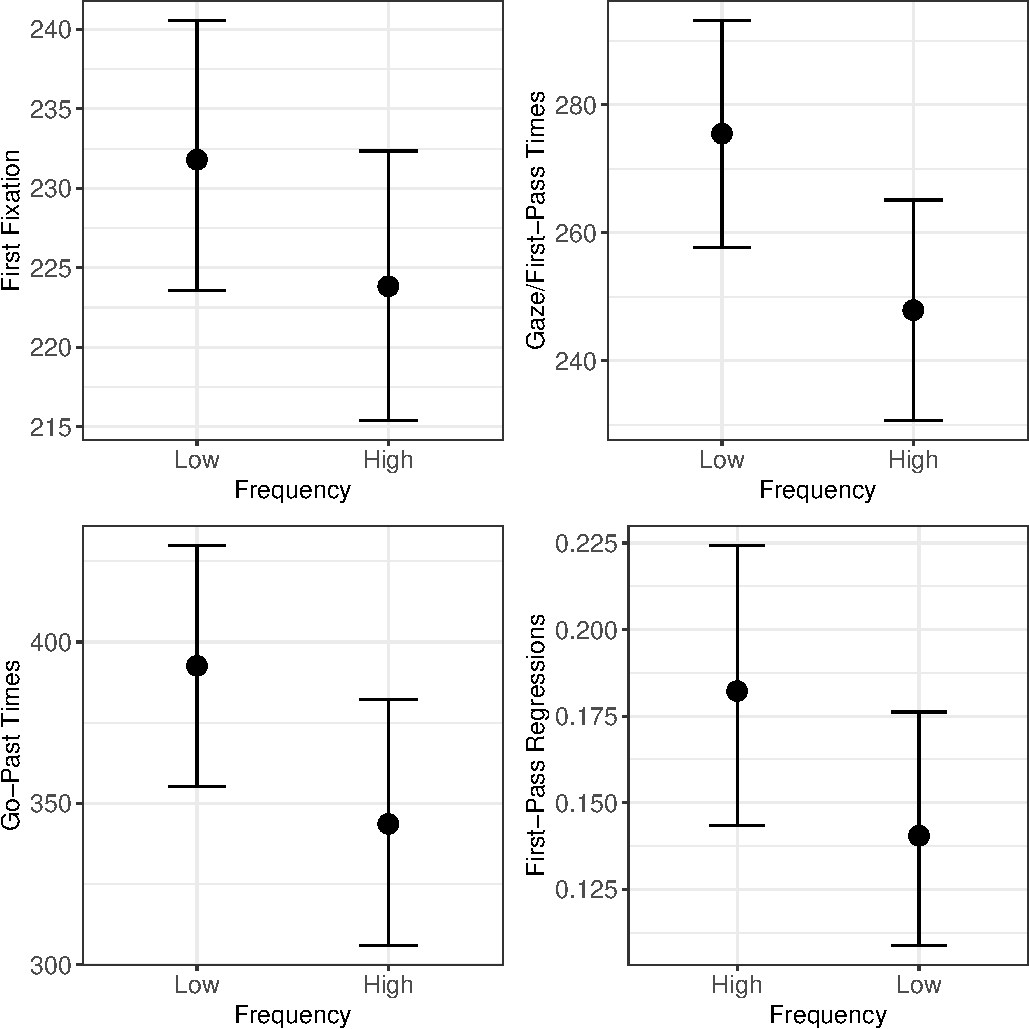
\includegraphics[keepaspectratio]{Chapters/Compound Nouns/staub_rep_ext_files/figure-pdf/fig-filleritemsall-1.pdf}}

}

\end{figure}%

\subsection{Discussion}\label{discussion-3}

In Experiment 4, we find an effect of plausibility only in first-pass
regressions. Interestingly, we do find an effect of plausibility in
first-fixation times for low-predictability items, but not for
high-predictability items. While this follows our theoretical prediction
that high-predictability items may be able to overcome the local
implausibility, the results are difficult to reconcile with the results
we see for first-pass regressions. For first-pass regressions, we
observe the opposite pattern: there is an effect of plausibility on
first-pass regressions for high-predictability items but not
low-predictability items. Thus overall it seems unlikely that
participants are accessing the holistic representation at the first
noun.

We also find no effect of plausibility for gaze duration or go-past
times, which was unexpected. It is unclear why we do not find a
consistent slowdown at the N1 region in locally implausible contexts.
One possibility is that perhaps the difference in plausibility for the
sentences wasn't as large as we expected. This seems unlikely given that
we normed the plausibility of the items beforehand, however it is
possible that the plausibility interpretations of the participants who
normed our data and the plausibility interpretations of the participants
who read our items had different sensitivities to the plausibility
manipulation.

It is also unlikely that the lack of an effect of implausibility is due
to measurement error, because we do find significant effects in all four
eye-tracking measures for the frequency manipulation in our filler
items.

Finally, the lack of a predictability effect suggests one of two
possibilities. First, it is possible that predictability does not drive
storage and that high-predictability compound nouns are not stored
holistically. Thus, upon reading the first noun in the compound, readers
simply access that noun and no other representations, thus generating a
slowdown because it is implausible. Alternatively, it is possible that
they are stored holistically, but that processing still unfolds
incrementally, and readers are not able to access the representation of
the compound noun until they've heard more than just the first noun in
the compound. Both of these results explain why we see no interaction
effect. We leave the task of disentangling these interpretations to
future work.

\section{Conclusion}\label{conclusion}

The present study examined the processing of compound nouns in locally
implausible and locally plausible contexts, specifically with respect to
their phrasal frequency and predictability. In Experiment 1 we
replicated Staub et al.
(\citeproc{ref-staubTimeCoursePlausibility2007}{2007}) using the A-maze
task (\citeproc{ref-boyceMazeMadeEasy2020}{Boyce et al., 2020}) and
found an increase in reaction time for the implausible condition at N1
region, but no interaction effect between plausibility and familiarity.
Additionally at the N2 region, we found an increase in reaction time for
the plausible condition relative to the implausible condition and a
decrease in reaction time for high-predictability items relative to
low-predictability items.

In Experiment 2 we extended Experiment 1 using predictability as the key
measure instead of phrasal frequency. Similar to Experiment 1, we found
an increase in reaction time for the implausible condition at the N1
region, but again found no interaction effect between plausibility and
predictability. Also similar to Experiment 1, we found an increase in
reaction time at the N2 region for the plausible condition and a
decrease in reaction time for the high-predictability items.

In Experiments 3 and 4 we replicated the two experiments with
eye-tracking. In Experiment 3, we found an effect of plausibility in
first fixation times, go-past times, and first-pass regressions. We also
found an interaction effect in go-past times such that high-frequency
items had higher go-past times in the implausible condition, but
low-frequency items did not. In Experiment 4, we find an effect of
plausibility in first-fixation times for low-predictability items (but
not high-predictability items) and an an effect of plausibility in
first-pass regressions for high-predictability items but not
low-predictability items.

Overall the results of experiments 1 and 2 suggest that the frequency or
predictability of the second noun in the compound (given the first noun)
has very little facilitatory effect on the processing of the first noun
in implausible contexts relative to plausible contexts. That is, the
increase in reaction time in the implausible condition for the N1 region
was not mediated by the frequency or predictability of the compound
noun. If participants were predicting the second noun upon reading the
first noun, then we might expect to have seen a decrease in reaction
time for the high-predictable items in the implausible condition
relative to the low-predictability items because the second noun always
eliminated the local implausibility.

Experiments 3 and 4 provide mixed-evidence. On one hand, there seems to
be a general effect of implausibility regardless of frequency or
predictability, however in some reading measures such as first-fixation
times in Experiment 4, predictability seemed to alleviate the slowdown
in the implausible condition. On the other hand, for other measures, the
slowdown generated by the implausible contexts was actually exacerbated
for high-frequency or high-predictability items (e.g., first-pass
regression times in both Experiment 3 and Experiment 4).

These results taken together suggest that in general there is an
increase in processing time for locally implausible contexts.
Additionally, this increase in processing time is not alleviated by the
frequency or predictability of the compound noun. That is, if compound
nouns are stored holistically and participants are able to access the
holistic representation at the first noun, then participants should have
been able to overcome the increased processing time for the locally
implausible contexts, because accessing the representation of the
compound noun would have eliminated the implausibility.

There are a few possible explanations for the results we found. One
possibility is simply that our high-predictability compound nouns aren't
stored holistically. It is important to note that our compound nouns
were the most predictable compound nouns in the entire Google
\emph{n}-grams corpus, thus it seems unlikely that they weren't
predictable enough to be stored, though it may be that English compound
nouns have relatively low predictability relative to other multi-word
phrases. The slowdown in the locally implausible context is not
surprising if the compound nouns are not stored holistically because
they would be processed incrementally. Thus readers would access the
first noun in the compound noun initially, generating a slowdown in the
locally implausible condition.

For example, in the sentence \emph{The zookeeper spread out the monkey
medicine that was in the enclosure}, \emph{monkey medicine} is quite
low-frequency, so it is unsurprising that it isn't stored holistically.
Thus participants must process the compound noun incrementally. Upon
reaching \emph{\ldots spread out the monkey\ldots{}}, there is an
increase in processing time due to the implausible nature of the
interpretation. On the other hand, \emph{mountain lion} is a frequent
compound noun, and thus could in theory be stored holistically. If that
were the case, in the sentence \emph{Jenny heard the huge mountain lion
pacing in its cage}, upon reaching \emph{mountain}, the reader may be
able to access the holistic representation \emph{mountain lion}, which
would eliminate the local implausibility because one cannot hear a
\emph{mountain}, but one certainly can hear a \emph{mountain lion}.
However, instead we see an increase in processing time regardless of
frequency of the compound noun. Further, we find analogous results for
predictability. That is, similarly, readers are not able to overcome the
increase in processing time when the first noun is highly predictive of
the second noun as well. Taken together, these results suggest that both
high-frequency compound nouns and high-predictability compound nouns may
not be stored holistically.

Another possibility is that the high-frequency and high-predictability
compound nouns are stored holistically, but the processing consequences
of them being stored holistically are such that there is no facilitatory
effect in the processing of the first noun in the compound noun. That
is, perhaps despite being stored holistically, readers might not commit
to accessing the holistic representation of the compound noun until
they've heard enough acoustics to eliminate possible competitors. For
example, after hearing \emph{peanut}, there are still a number of
possible words other than \emph{butter} that could occur. Even though
\emph{butter} has a high probability of occurring after \emph{peanut},
it would be costly to the reader to commit to \emph{butter} and then
have to reinterpret the sentence upon hearing a different word. Thus,
the reader may avoid committing to \emph{peanut butter} until they are
confident that it is what the speaker intended to say.

An interesting question that comes out of this is at what point readers
do access the holistic representation? For example, in the case of
\emph{peanut butter}, do participants need to hear the entire phrase
before accessing the holistically stored representation? To address this
question, we turn to a literature that has a much longer history:
word-recognition. A similar question has been asked on the word-level
for over a century: Do people recognize a word by its component letters
or by the whole (\citeproc{ref-goel2013wholegreatersum}{Goel et al.,
2013}; \citeproc{ref-huey1908psychologypedagogyreading}{Huey, 1908};
\citeproc{ref-johnston1974perceptionletterswords}{Johnston \&
McClelland, 1974};
\citeproc{ref-pelli2003remarkableinefficiencyword}{Pelli et al., 2003};
\citeproc{ref-reicher1969perceptualrecognitionfunction}{Reicher, 1969};
\citeproc{ref-wheeler1970processeswordrecognition}{Wheeler, 1970})? For
example, readers are more accurate at identifying a letter when it
occurs within a word
(\citeproc{ref-johnston1980experimentaltestshierarchical}{Johnston \&
McClelland, 1980}). Additionally, Goel et al.
(\citeproc{ref-goel2013wholegreatersum}{2013}) demonstrated that a
word-recognition model that identifies the word based on the whole image
performs better than a model that detects individual characters and then
combines them. On the other hand, Pelli et al.
(\citeproc{ref-pelli2003remarkableinefficiencyword}{2003}) demonstrated
that human word-recognition accuracy is closer in accuracy to a
feature-based model, than a holistic model. In disentangling these
results, Johnston \& McClelland
(\citeproc{ref-johnston1980experimentaltestshierarchical}{1980})
proposed a hierarchical model where in features were recognized, then
letters, then words. They found that this model accounted for the result
that words are identified better in word-contexts than in isolation
because identifying the word maintained the activation of the
letter-representations longer than simply identifying the letter in
isolation. These results suggest that word-recognition does involve
recognizing each of the parts of the word, but it is still unclear how
many of the parts of the word must be recognized to give rise to the
recognition of the entire word.

Word-recognition is further complicated by the question of when a word
is activated over its competitors. For example, words with many
phonological neighbors are harder to recognize in noise and show longer
lexical decision times than those with fewer phonological neighbors
(where phonological neighbors are words that vary by exactly 1 phoneme
from the target word,
\citeproc{ref-goldinger1989priminglexicalneighbors}{Goldinger et al.,
1989}). Similar effects have been observed in visual word-recognition as
well (\citeproc{ref-coltheart1977access}{Coltheart et al., 1977}). These
results suggest that readers are able to recognize a word before seeing
all of the parts of the word. That is, if it was the case that readers
wait until reading all of the letters to process a word, then the number
of phonological competitors should not matter. However, if readers
process the word at the point in which it is unlikely that the text
refers to a different word, regardless of whether all the letters have
been processed, then a word with fewer competitors will be activated
earlier.

These results taken together provide some inspiration for how holistic
representations of phrases may be activated: a holistically stored
phrase may be processed incrementally, and the holistic representation
may be accessed at the point where the evidence for the holistic
representation of the phrase vastly outnumbers the evidence for its
competitors. For example, the holistic representation for \emph{peanut
butter} may be accessed once evidence for \emph{peanut butter} greatly
outnumbers the evidence for \emph{peanut} followed by some other word.
However it would be interesting for future work to further examine
whether the recognition of holistically stored phrases parallels the
recognition of words. This evidence may not be enough even for
high-predictability compound nouns, because the first noun is still
occasionally followed by other words. Although this account may make
exceptions for extremely predictable words, such as \emph{Habeus
Corpus}, where there are extremely few competitors.

Finally, with respect to the increase in reaction time at the N2 region
in the plausible condition that we found in Experiments 1 and 2, we do
not see this effect in Experiments 3 and 4, suggesting that this effect
may be a task-specific effect. This result suggests that in the maze
task, participants may have a bias to analyze the first noun as the head
noun and then have to reinterpret the sentence once it is clear that the
noun is not the head noun. Further, since we don't see the same effect
in the implausible condition, participants may not fully commit to an
interpretation that is implausible.

In summary, the present study contributes to the current theories of
sentence processing by demonstrating that during sentence processing,
readers do not seem to access the holistic representation at the first
noun (because then they would be able to overcome the implausibility).
Instead, it is possible that high-frequency and high-predictability
compound nouns are either not stored holistically, or if they are stored
holistically, perhaps readers don't access the holistic representation
until they have heard sufficient evidence for that representation. That
is, even though \emph{peanut} is predictive of \emph{butter}, there are
still many other words that can occur after \emph{peanut}. Thus, readers
may not access the holistic representation until they hear enough of the
compound noun to rule out other competing possibilities.

\bookmarksetup{startatroot}

\chapter{\texorpdfstring{The effects of frequency and predictability on
the recognition of \emph{up} in English verb+up
collocations}{The effects of frequency and predictability on the recognition of up in English verb+up collocations}}\label{the-effects-of-frequency-and-predictability-on-the-recognition-of-up-in-english-verbup-collocations}

\section{Introduction}\label{introduction-2}

When a listener hears the phrase \emph{trick or treat}, do they process
it compositionally, processing each word individually before combining
them into a single parse? Or do they access a single holistically stored
representation of the phrase from memory? This question of to what
extent larger-than-word constructions can be stored and accessed
holistically is one that psycholinguists have been interested in for
quite some time (\citeproc{ref-bybee2003}{Bybee, 2003}; e.g.,
\citeproc{ref-bybee2001}{Bybee \& Hopper, 2001};
\citeproc{ref-goldbergConstructionsNewTheoretical2003}{Goldberg, 2003};
\citeproc{ref-nooteboomStorageComputationLanguage2002}{Nooteboom et al.,
2002}; \citeproc{ref-stembergerFrequencyLexicalStorage1986}{Stemberger
\& MacWhinney, 1986},
\citeproc{ref-stembergerAreInflectedForms2004}{2004}).

Throughout the years different theories have argued for different
degrees of holistic storage, with two theories in particular dominating
the field. On one hand, Chomskyan theories (e.g.,
\citeproc{ref-chomsky1965}{Chomsky, 1965};
\citeproc{ref-pinker2002}{Pinker \& Ullman, 2002}) have proposed that
only necessary items (e.g., items that can't be formed compositionally)
are stored.\footnote{Although some theories (e.g.,
  \citeproc{ref-pinker2002}{Pinker \& Ullman, 2002}) have accepted that
  some very high-frequency items may be stored due to human memory, but
  these theories are much more conservative about what is stored
  compared to usage-based theories.} On the other hand, usage-based
theories (e.g., \citeproc{ref-bybee2003}{Bybee, 2003}) have proposed
that many items that could in principle be formed compositionally can be
stored under certain usage-based conditions, such as frequency of use.

Traditional Chomskyan theories (e.g.,
\citeproc{ref-chomsky1965}{Chomsky, 1965};
\citeproc{ref-pinker2002}{Pinker \& Ullman, 2002}) have argued that
processing multi-word phrases is completely compositional: each piece is
accessed individually and then combined to form the larger meaning. Some
exceptions are reserved for idioms and other outliers, which can't be
formed compositionally. More specifically, Chomskyan views of storage
argue that whether an item is stored is determined purely by the degree
of compositionality. According to these theories, if a multi-word
expression can be composed from its parts then there is no need to
holistically store the expression, and thus it is not stored
holistically. For example since \emph{I don't know} can be processed
compositionally, it would be processed by composing a representation
from each of the individual words, \emph{I, don't,} and \emph{know}. On
the other hand, \emph{kicked the bucket} would be stored holistically
because there's very little relationship between the meaning of the
individual words and the meaning of the expression (i.e., it's
non-compositional).

Chomskyan theories of storage gained popularity partly because storage
was thought to be a valuable resource that was taken up only by units
that necessitated storage. This was perhaps influenced by the limited
storage space of sophisticated computers at the time. In recent times,
however, we've learned that the brain may have dramatically more space
for storage than we had previously realized, with an upper bound of
10\textsuperscript{8432} bits
(\citeproc{ref-wangDiscoveringCapacityHuman2003}{Wang et al., 2003}).
This is magnitudes larger than any current estimate of how much storage
language requires.\footnote{Indeed, Mollica \& Piantadosi
  (\citeproc{ref-mollicaHumansStoreMegabytes2019}{2019}) estimated that,
  in terms of linguistic information, humans store only somewhere
  between one million and ten million bits of information, meaning that
  even their upper estimate is well within the capacity of the brain.}
Considering this, it might not come as a surprise that there has been a
rise in support for usage-based theories of holistic storage over the
past few decades
(\citeproc{ref-ambridgeStoredAbstractionsRadical2020}{Ambridge, 2020};
\citeproc{ref-baayenDutchInflectionRules2002}{H. Baayen et al., 2002};
\citeproc{ref-bybee2003}{Bybee, 2003}; \citeproc{ref-bybee2001}{Bybee \&
Hopper, 2001}; \citeproc{ref-bybeeEffectUsageDegrees1999}{Bybee \&
Scheibman, 1999}; \citeproc{ref-kapatsinski2018}{Kapatsinski, 2018};
\citeproc{ref-kapatsinskiFrequencyEmergencePrefabs2009}{Kapatsinski \&
Radicke, 2009}; \citeproc{ref-morganAbstractKnowledgeDirect2016}{Morgan
\& Levy, 2016a};
\citeproc{ref-stembergerFrequencyLexicalStorage1986}{Stemberger \&
MacWhinney, 1986}, \citeproc{ref-stembergerAreInflectedForms2004}{2004};
\citeproc{ref-zangParafovealProcessingChinese2024}{Zang et al., 2024}).

Usage-based theories posit that more than just non-compositional items
(e.g., multi-word expressions) may be stored holistically in the
lexicon, arguing that storage is driven by usage-based factors. For
example, factors like frequency or predictability of the phrase may
influence whether the phrase is stored holistically or not. According to
these theories, in addition to idioms and non-compositional items,
multi-word phrases such as \emph{I don't know} may also be stored
holistically if they are used frequently enough (e.g.,
\citeproc{ref-ambridgeStoredAbstractionsRadical2020}{Ambridge, 2020};
\citeproc{ref-arnonMoreWordsFrequency2010}{Arnon \& Snider, 2010};
\citeproc{ref-kapatsinski2018}{Kapatsinski, 2018};
\citeproc{ref-kapatsinskiFrequencyEmergencePrefabs2009}{Kapatsinski \&
Radicke, 2009};
\citeproc{ref-leeFrequencyEffectsMorphologisation2015}{Lee \&
Kapatsinski, 2015};
\citeproc{ref-morganAbstractKnowledgeDirect2016}{Morgan \& Levy, 2016a};
\citeproc{ref-stembergerFrequencyLexicalStorage1986}{Stemberger \&
MacWhinney, 1986}, \citeproc{ref-stembergerAreInflectedForms2004}{2004};
\citeproc{ref-tomaselloConstructingLanguageUsagebased2005}{Tomasello,
2005}).

While it has become a dominant view in the field that at least some
multi-word items are stored, it remains unclear what exactly the size of
the units being stored is and, more so, what the factors driving storage
are. Further, if multi-word representations are stored holistically,
what are the consequences of this in terms of language processing?

\subsection{Evidence of Holistic
Storage}\label{evidence-of-holistic-storage}

There is no shortage of evidence for holistic multi-word storage (e.g.,
\citeproc{ref-bybeeEffectUsageDegrees1999}{Bybee \& Scheibman, 1999};
\citeproc{ref-christiansenMoreWordsRole2017}{Christiansen \& Arnon,
2017}; \citeproc{ref-stembergerFrequencyLexicalStorage1986}{Stemberger
\& MacWhinney, 1986},
\citeproc{ref-stembergerAreInflectedForms2004}{2004};
\citeproc{ref-zwitserloodProcessingRepresentationMorphological2018}{Zwitserlood,
2018}), especially in the phonology literature. For example, Bybee \&
Scheibman (\citeproc{ref-bybeeEffectUsageDegrees1999}{1999})
demonstrated that the word \emph{don't} is reduced to a larger extent in
the phrase \emph{I don't know} than in other phrases containing
\emph{don't}. In other words, the phrase \emph{I don't know} seems to
have its own mental representation. If it was the case that the
representation of \emph{don't} in \emph{I don't know} was the same as
the representation of \emph{don't} in other contexts, then one would
expect \emph{don't} to be equally reduced in both cases (which is
contrary to the finding in
\citeproc{ref-bybeeEffectUsageDegrees1999}{Bybee \& Scheibman, 1999}).
Similarly, in Korean, certain consonants undergo tensification when they
occur after the future marker -\emph{l}. The rate of this tensification
is higher in high-frequency phrases than low-frequency phrases, further
suggesting that high-frequency phrases may be stored holistically
(\citeproc{ref-yiEumun2002}{Yi, 2002}).

In addition to the phonology literature, the Psycholinguistics
literature has also provided an abundance of evidence for multi-word
storage. For example, Siyanova-Chanturia et al.
(\citeproc{ref-siyanova-chanturiaSeeingPhraseTime2011}{2011})
demonstrated that binomial phrases (e.g., \emph{cat and dog}) are read
faster in their more frequent ordering than in their less frequent
ordering. Further, in a follow-up study, Morgan \& Levy
(\citeproc{ref-morganAbstractKnowledgeDirect2016}{2016a}) demonstrated
that these ordering preferences for frequent binomials are not due to
abstract ordering preferences (e.g., a preference for short words before
long words), but are rather driven by experience with the specific
binomial (i.e., how frequent each binomial ordering is), providing
additional evidence that frequent phrases are stored holistically.

Similarly, Arnon \& Snider
(\citeproc{ref-arnonMoreWordsFrequency2010}{2010}) demonstrated that
frequent multi-word phrases are read faster than lower frequency
multi-word phrases, even after accounting for the frequency of the
individual words. This suggests that humans are sensitive to the
frequencies of multi-word phrases. Further, in language production
humans are also sensitive to the frequency of multi-word phrases. In a
production study, Janssen \& Barber
(\citeproc{ref-janssenPhraseFrequencyEffects2012}{2012}) found that
participants produced frequent multi-word phrases faster than lower
frequency phrases, even after taking into account the frequencies of the
individual words.

Further, there is also evidence of multi-word storage from the learning
literature (\citeproc{ref-bannardStoredWordSequences2008}{Bannard \&
Matthews, 2008};
\citeproc{ref-siegelmanAdvantageStartingBig2015}{Siegelman \& Arnon,
2015}). For example, Siegelman \& Arnon
(\citeproc{ref-siegelmanAdvantageStartingBig2015}{2015}) demonstrated
that learning is facilitated by attending to the whole utterance, as
opposed to attending to each individual word. Specifically, they used an
artificial language paradigm to examine adult L2 learners' ability to
learn grammatical gender. They found that adults learn grammatical
gender better when they are presented with unsegmented utterances rather
than segmented utterances. In other words, attending to the entire
utterance, rather than learning to compose the utterance word-by-word,
facilitated their learning. It seems plausible that if the entire
utterance is being attended to, then participants may be learning (i.e.,
storing) the entire utterance initially. Further, storing
larger-than-word chunks may possibly be facilitating the learning of
grammatical gender in their study.

\subsection{What Drives Storage?}\label{what-drives-storage}

Despite the evidence of multi-word holistic storage, however, it is
still largely unclear what factors drive storage. Humans seem to be
sensitive to a variety of statistical information, including both
frequency (e.g., \citeproc{ref-bybeeEffectUsageDegrees1999}{Bybee \&
Scheibman, 1999};
\citeproc{ref-kapatsinskiFrequencyEmergencePrefabs2009}{Kapatsinski \&
Radicke, 2009};
\citeproc{ref-leeFrequencyEffectsMorphologisation2015}{Lee \&
Kapatsinski, 2015}; \citeproc{ref-mayeLearningPhonemesMinimal2000}{Maye
\& Gerken, 2000}) and predictability (e.g,
\citeproc{ref-olejarczukDistributionalLearningErrordriven2018}{Olejarczuk
et al., 2018};
\citeproc{ref-ramscarChildrenValueInformativity2013}{Ramscar et al.,
2013}).

Traditionally, frequency has been assumed to be the driving factor
behind multi-word storage. Indeed, most of the examples of storage given
so far have been with respect to frequency. Perhaps the most famous
series of studies demonstrating this were conducted by Bybee
(\citeproc{ref-bybee2003}{Bybee, 2003}; \citeproc{ref-bybee2001}{Bybee
\& Hopper, 2001}; \citeproc{ref-bybeeEffectUsageDegrees1999}{Bybee \&
Scheibman, 1999}). In a series of studies, Bybee and colleagues
demonstrated that a variety of words are reduced more in high-frequency
contexts than low-frequency contexts (additionally see
\citeproc{ref-kapatsinskiHierarchicalInferenceSound2021}{Kapatsinski,
2021} for further discussion of this). For example, in addition to the
earlier examples, \emph{going to} can be reduced in the frequent future
marker, \emph{gonna}, but not in the less frequent verb phrase
construction describing motion (e.g., *\emph{gonna the store},
\citeproc{ref-bybee2003}{Bybee, 2003}). This mirrors patterns we see on
a word-level (which for the most part must be stored). For example, the
reduction of vowels to schwa in English is more advanced in
high-frequency words than low-frequency words
(\citeproc{ref-bybee2003}{Bybee, 2003};
\citeproc{ref-hooperWordFrequencyLexical1976a}{Hooper, 1976}). In other
words, for both words and phrases, sound reduction advances more quickly
as a function of frequency (i.e., high-frequency phrases and
high-frequency words are both more reduced than their lower frequency
counterparts). While this is not surprising for words (which most
theories posit have separate representations), it is surprising for
phrases which don't necessarily have to be stored holistically.

On the other hand, predictability has not been directly examined much by
the Psycholinguistics literature within the context of holistic
multi-word storage (c.f.
\citeproc{ref-odonnellFragmentGrammarsExploring2009}{O'Donnell et al.,
2009}). Additionally, the previous chapter demonstrated that
predictability didn't alleviate the effects of local implausibility in
reading. To refresh the readers memory, in the previous chapter I
examined whether participants were slower to select the first noun in
high-predictability compound nouns in locally implausible contexts
(i.e., contexts where the first noun in the compound is implausible but
where the second noun eliminates the implausibility; see the below
sentences) relative to high-predictability compound nouns in locally
plausible contexts.

\begin{exe}
\ex
\begin{xlist}
\ex Jimmy spread out the peanut butter. \hfill \emph{high-predictability, plausible}
\ex Jimmy picked up the peanut butter. \hfill \emph{high-predictability, implausible}
\end{xlist}
\end{exe}

\noindent Note that in the implausible condition, the second noun always
eliminates the implausibility (i.e., \emph{spread out the peanut} is
implausible, but \emph{spread out the peanut butter} is not). If
high-predictability compound nouns are stored holistically, participants
may be able to access the full compound noun upon encountering the first
noun, thus overcoming the local implausibility effect (since the second
noun in the compound always eliminates the implausibility). The results
suggested that the first noun in the compound nouns was read slower in
the implausible condition than in the plausible condition.
Interestingly, this slowdown was roughly the same regardless of the
predictability of the compound noun. That is, there was an increase in
reaction time for selecting the first noun in the compound in the
implausible condition (relative to the plausible condition) regardless
of the predictability of the second noun in the compound noun. Their
results suggest that either predictability doesn't drive the holistic
storage of compound nouns or that it doesn't facilitate processing in
this manner. However they noted that this may be a task effect, since
they used the maze task as opposed to an eye-tracking task.

Despite the lack of direct evidence of predictability in the role of
multi-word storage, however, predictability has been shown to play a
crucial role in learning
(\citeproc{ref-olejarczukDistributionalLearningErrordriven2018}{Olejarczuk
et al., 2018};
\citeproc{ref-ramscarChildrenValueInformativity2013}{Ramscar et al.,
2013}; \citeproc{ref-saffranStatisticalLearning8MonthOld1996}{Saffran et
al., 1996}). For example, Olejarczuk et al.
(\citeproc{ref-olejarczukDistributionalLearningErrordriven2018}{2018})
demonstrated that when learning new phonetic categories, learners don't
just pay attention to co-occurrence rates, but actively try to predict
upcoming sounds, suggesting that the learning of phonetic categories is
also driven by prediction (i.e., the predictability of a given sound
within a context). Further, in learning new words, Ramscar et al.
(\citeproc{ref-ramscarChildrenValueInformativity2013}{2013})
demonstrated that children are sensitive to how predictable a cue is of
an outcome (e.g., a high-frequency cue will be ignored if it isn't
predictive of a specific outcome). Additionally, word-segmentation
(i.e., learning which segments in an utterance are words) is also highly
sensitive to predictability
(\citeproc{ref-saffranStatisticalLearning8MonthOld1996}{Saffran et al.,
1996}). In their classic paper, Saffran et al.
(\citeproc{ref-saffranStatisticalLearning8MonthOld1996}{1996})
demonstrated that children keep track of transitional probabilities -- a
measurement of predictability -- to segment the speech stream. While
these are studies examining learning, not storage, the units that we
learn may likely be the units we store. If predictability drives what we
learn, it may also drive what we store.

Thus, the current literature presents strong evidence for the role of
frequency in the storage of multi-word phrases, as well as suggests the
possibility of a further influence of predictability. However, it
remains unclear to what extent each of these factors drives storage and
whether they interact at all with each other.

\subsection{Representation of Stored
Units}\label{representation-of-stored-units}

Given the evidence that a lot more may be stored than previously
thought, another important question to consider is what the internal
representations of these units is. Specifically, do the stored units
maintain their own internal representation with respect to their
component parts? For example, it is possible that the representation of
high-frequency phrases, such as \emph{pick up,} retains the
representations of the component parts \emph{pick} and \emph{up}
(Figure~\ref{fig-lossinternalstructure}). On the other hand, it is
possible that the phrase lacks internal representation of the component
parts, either because it was lost over time or because it was not
learned to begin with.

Indeed, there seems to be some evidence that multi-word phrases may not
have a fully intact internal structure with respect to their component
parts. For example, Kapatsinski \& Radicke
(\citeproc{ref-kapatsinskiFrequencyEmergencePrefabs2009}{2009})
demonstrated that in high-frequency V+\emph{up} constructions, it is
harder to recognize the segment \emph{up} (with respect to
medium-frequency V+\emph{up} constructions). This suggests that those
items may have a holistic representation that has lost some of its
internal structure. In their study, participants were given different
auditory sentences and tasked with pressing a button immediately if they
heard the segment \emph{up}. Interestingly, they found that
recognizability of \emph{up} follows a U-shaped pattern with respect to
the frequency of the phrase. That is, participants were slow to
recognize \emph{up} in low-frequency phrasal verbs, but for
medium-high-frequency phrasal verbs they were quicker to recognize
\emph{up}. However, upon reaching the highest frequency words
participants once again grew slower to recognize \emph{up} (See
Figure~\ref{fig-kapatsinskiplot}). Though it's important to note that
the original paper does not take into account predictability. It's
unclear how to account for the increase in recognition time for the
highest frequency items if there is no loss of internal representation
of those items.

A visualization of what a stored representation with and without
internal structure may look like is presented in
Figure~\ref{fig-lossinternalstructure}. The left tree represents the
phrase \emph{pick up} stored with its internal structure still intact,
whereas the right tree represents \emph{pick up} stored without internal
structure. Note that both trees are examples of a holistically stored
representation. The key difference is whether the internal structure
remains intact in the holistic representation. The results from
Kapatsinski \& Radicke
(\citeproc{ref-kapatsinskiFrequencyEmergencePrefabs2009}{2009}) suggest
that for high-frequency verb+\emph{up} collocations, their
representation may be more similar to the tree on the right, since
participants were slower to recognize \emph{up}. We will revisit this
point in the discussion section in more detail.

\begin{figure}[htbp]

\caption{\label{fig-kapatsinskiplot}The U-shaped effect of the frequency
of verb+\emph{up} constructions on the speed with which \emph{up} is
detected, reproduced from Kapatsinski \& Radicke
(\citeproc{ref-kapatsinskiFrequencyEmergencePrefabs2009}{2009}).}

\centering{

\includegraphics[width=1\linewidth,height=\textheight,keepaspectratio]{Chapters/Recognizability/Write-up/Figures/kapatsinskiradicke_graph.pdf}

}

\end{figure}%

\begin{figure}[htbp]

\caption{\label{fig-lossinternalstructure}A diagram of two ways the word
\emph{pick up} could be stored. The left tree demonstrates a stored
representation of \emph{pick up}, where the internal structure is still
intact. The right tree demonstrates a holistically stored unit, where
there is a loss of internal structure. Note that both of these are
stored structures, as opposed to a compositional representation of
\emph{pick up} which would be comprised of the individual
representations \emph{pick} and \emph{up}.}

\centering{

\includegraphics[width=0.5\linewidth,height=\textheight,keepaspectratio]{Chapters/Recognizability/Write-up/Figures/storage_syntax_tree.pdf}

}

\end{figure}%

It's worth noting that in the case of phrasal verbs like \emph{pick up},
it can't be the case that the entire internal representation is lost
because it is possible to syntactically alternate it (e.g., \emph{pick
up the cup} vs \emph{pick the cup up}). However, it is possible that
semantic or lemma information is lost in the holistic representation.
That is, it is possible that syntactic and/or morphological information
may be preserved even if semantic or lemma information is lost. In other
words, loss of internal representation may happen at different levels as
opposed to being an all-or-nothing process.

\subsection{Present Study}\label{present-study}

The present study examines the factors that drive storage and the
representations of stored items by extending Kapatsinski \& Radicke
(\citeproc{ref-kapatsinskiFrequencyEmergencePrefabs2009}{2009}) to look
at the effects of both frequency, predictability, and their interaction
on the processing of V+\emph{up} phrases. Similar to Kapatsinski \&
Radicke (\citeproc{ref-kapatsinskiFrequencyEmergencePrefabs2009}{2009})
, participants are tasked with pressing a button once they hear the
segment \emph{up} (which in our study occurs either as a particle within
verb phrases, e.g., \emph{pick up}, or part of a word, e.g.,
\emph{puppet}), but in our case the stimuli varied in frequency,
predictability, and whether they were a phrasal verb or not. Since both
frequency and predictability effects are rather robust in the
literature, we should at the very least see a negative correlation
between frequency and predictability and recognition time (up to perhaps
a certain point, where recognition time may increase). Further, if
predictability is not a driving factor of storage, we should see an
increase in recognition times for only the most \emph{frequent} phrases.
On the other hand, if predictability does drive storage, we may see an
increase in reaction time for both frequent and predictable phrases.

\section{Methods}\label{methods-4}

\subsection{Participants}\label{participants-4}

Participants were recruited through the University of California, Davis
Linguistics/Psychology Human Subjects Pool. 350 people participated in
this study and were compensated in the form of course credit. All
participants self-reported being native English speakers. Additionally,
44 participants were excluded due to an accuracy score below our
threshold of 70\%, leaving a total of 306 participants for the data
analysis.

\subsection{Materials}\label{materials-2}

We searched the Google \emph{n}-grams corpus
(\citeproc{ref-linSyntacticAnnotationsGoogle2012}{Lin et al., 2012}) for
the most predictable and the highest frequency phrases that matched our
criteria of containing a verb immediately followed by the word
\emph{up}. We operationalized predictability as the odds ratio of the
probability of \emph{up} occurring immediately after the verb to the
probability of any other word occurring (Equation~\ref{eq-logodds}).

\begin{equation}\phantomsection\label{eq-logodds}{
\frac{\mathrm{count(\textit{Verb+up})}}{\mathrm{count(\textit{Verb})} - \mathrm{count(\textit{Verb+up})}} 
}\end{equation}

In non-mathematical terms, the above equation quantifies how likely
\emph{up} is to follow after the verb relative to every other word that
could follow. For example, the odds ratio of \emph{pick up} would be the
number of times the entire verb phrase occurs -- \emph{pick up} --
divided by the number of times the verb -- \emph{pick} -- occurs without
\emph{up} following it.

For the purposes of the present study, we gathered a variety of phrases
that varied in both their predictability and frequency and their
combination. In order to do this, we extracted the 50 most frequent
Verb+\emph{up} items and the 50 most predictable ones. Next, we selected
100 more by randomly sampling from the remaining items. In order to
ensure stable predictability estimates we eliminated words that a
college-aged speaker wouldn't have heard more than 10 times.\footnote{Levy
  et al. (\citeproc{ref-levyProcessingExtraposedStructures2012}{2012})
  extrapolated that the average college-aged speaker has heard about 350
  million words in their lifetime. Thus we excluded items that had a
  frequency smaller than 10 per 350 million.} We then visually inspected
the data to confirm that our data spanned across both the frequency and
predictability continuum. This distribution is presented in
Figure~\ref{fig-stimplot}.

\begin{figure}[htbp]

\caption{\label{fig-stimplot}log-predictability by log-frequency (per
million) plot of our items.}

\centering{

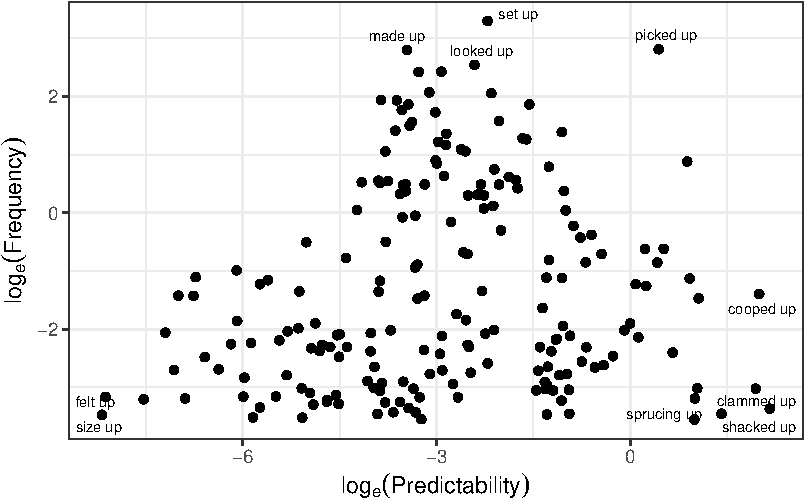
\includegraphics[width=0.9\linewidth,height=\textheight,keepaspectratio]{Chapters/Recognizability/Write-up/quarto-writeup_files/figure-pdf/fig-stimplot-1.pdf}

}

\end{figure}%

Phrasal verbs show a syntactic alternation that is not present in all
verb+\emph{up} collocations (e.g., in the example below \emph{lightened
up the room} is fine, but \emph{lightened the room up} is weird at
best). It is possible that due to this syntactic alternation, phrasal
verbs may be stored regardless of frequency and predictability. This is
because in order to properly use phrasal verbs, a speaker must be aware
of the syntactic alternation, which can't simply be predicted
compositionally (e.g., some V+\emph{up} phrases are phrasal verbs, while
other V+\emph{up} phrases are not phrasal verbs\footnote{Note that this
  largely correlates with whether the verb is transitive or not.}).
Thus, we additionally coded our stimuli for whether they were phrasal
verbs or not. This coding was done based on whether they could
syntactically alternate between having the noun within the verb phrase
and having the noun immediately after the verb phrase. For example,
since both \emph{pick the cat up} and \emph{pick up the cat} are
grammatical, \emph{pick up} was classified as a phrasal verb. Each item
was checked by two of the authors. Disagreement was easily resolved by
discussion and an agreement was reached for every item.

\begin{exe} 
\ex
  \begin{singlespace}
  \begin{xlist}
    \ex The student lightened up the room. \\
    \ex ??The student lightened the room up. \\
  \end{xlist}
  \end{singlespace}
\end{exe}

We also searched the same corpus for words that contained the segment
\emph{up} (e.g., \emph{cupcake}). In order to gather a subset of words
that roughly matches the frequency range of our experimental stimuli, we
extracted the 50 most frequent words, then sampled from the rest of the
dataset to gather an additional 100 words. These 350 items together
comprise our stimuli.

For each item, we constructed two sentences: one sentence which
contained \emph{up}, and one sentence that was identical except that it
didn't include the segment \emph{up.} For words, the entire word was
replaced. For phrases, \emph{up} was simply deleted if possible (e.g.,
\emph{clean up} replaced with \emph{clean}). If this resulted in an
awkward sentence, the entire phrase was replaced. An example is given
below.

\begin{exe} 
\ex
  \begin{xlist}
  \begin{singlespace}
    \ex He picked up the phone and answered the call. \\
    \ex He grabbed the phone and answered the call. \\
  \end{singlespace}
  \end{xlist}
\end{exe}

In summary, our stimuli were comprised of 200 Verb+\emph{up} phrases
that varied in both frequency and predictability, 150 words that
contained \emph{up}, and 350 filler sentences which were matched with
our experimental sentences with the exception of having \emph{up}
replaced.

After creating the sentences, a native English speaker then recorded
each sentence in a random order to minimize any list effect. We
subsequently equalized the amplitude such that every sentence was
roughly the same loudness.

\subsection{Procedure}\label{procedure-3}

Participants were presented with audio sentences via Pavlovia
(\url{https://pavlovia.org/}), a website for presenting PsychoPy
experiments (\citeproc{ref-peirce2019psychopy2}{Peirce et al., 2019}).
Each participant was presented with 3 practice trials and then 350
sentences. While we had a total of 700 sentences, participants didn't
see both the filler and experimental sentence for the same item, thus
they only saw half of the stimuli. The order of the sentences was random
and exactly half of the sentences contained the target segment (to avoid
biasing the participants towards a specific response). Participants were
instructed to press a key as soon as they heard the segment \emph{up},
or to press a separate key at the end of the sentence if they did not
hear the target segment in the sentence. We then recorded their reaction
time of the button press. The experiment took approximately 40 minutes.

\section{Results}\label{results-4}

The data was analyzed using General Additive Mixed models, as
implemented in the \emph{mgcv} package
(\citeproc{ref-wood2011fast}{Wood, 2011}) within the R programming
environment (\citeproc{ref-Rpackage}{R Core Team, 2022}).\footnote{For
  complete details of our analyses, please refer to the following link:
  \url{https://github.com/znhoughton/dissertation_writeup/tree/master/Chapters/Recognizability/Analysis}.}
General Additive Mixed Models are models that allow us to model our
outcome variable as a combination of the predictors. GAMMs differ from
generalized linear regression models in that they allow the predictors
to be modeled as non-linear functions, similar to polynomial regression.
Specifically, in a Generalized Additive Mixed Model, beta-coefficients
are replaced with a smooth function, which is a combination of splines.
The more splines that we include, the more wiggly our line will be. In
order to avoid overfitting, GAMMs also include a penalty term,
\(\lambda\), which can be modified to penalize more wiggly lines that
aren't justified by the data. While the predictors are allowed to vary
non-linearly, the linking function in our case was linear (i.e.,
response time varied linearly with the spline functions). Our decision
to use GAMMs was driven by our hypothesis that recognition times may
vary non-linearly as a function of frequency and/or predictability (as
suggested by
\citeproc{ref-kapatsinskiFrequencyEmergencePrefabs2009}{Kapatsinski \&
Radicke, 2009}).

For all of our models, the dependent variable was the time it took for
participants to react to the onset of the target segment in experimental
sentences/sentences containing \emph{up} (i.e., the time it took
participants to press the button after hearing \emph{up}).

In order to visualize the surface of the interaction effect between
frequency and predictability, we first ran a model with our independent
variable as the interaction between log-predictability and
log-frequency, which was allowed to vary non-linearly, and duration of
the segment, which was not allowed to vary non-linearly. Additionally,
we also included random intercepts for participant, trial, and item, as
well as random by-participant slopes for predictability, frequency,
their interaction, and trial. All our random-effects were allowed to be
wiggly (non-linear). Our model formula is included below in
Equation~\ref{eq-gamminteraction}. This model allows us to visualize the
surface of the interaction effect. Note that in GAMMs, the syntax
\texttt{ti()} is used to model the interaction effects since it produces
a tensor product interaction from which the main-effects have been
excluded. On the other hand \texttt{te()} models the full tensor product
smooth without the main-effects excluded. Thus when modeling the
main-effects with the interaction effect we use \texttt{ti()} and when
modeling the surface (that is, without separating the main-effects from
the interaction) we use \texttt{te()}.

\begin{equation}\phantomsection\label{eq-gamminteraction}{
\begin{aligned}log(RT) & \sim te(Predictability, Frequency) + Duration + s(participant, bs = \text{`}re\text{'}) + \\ & s(Item, bs = \text{`}re\text{'}) + s(trial, bs = \text{`}re\text{'}) + \\ & s(Predictability, Frequency, participant, bs = \text{`}re\text{'}) \end{aligned}
}\end{equation}

The results of this model are presented in Table~\ref{tbl-gamModelTab}
and visualized in Figure~\ref{fig-gam2dplot1}. We found no significant
effect of the tensor product smooth.\footnote{We also examined the
  interaction between frequency and predictability on accuracy (whether
  they correctly responded to whether \emph{up} was present in the
  sentence) and similarly found no significant effect.} Although the
tensor product smooth for the interaction effect was not significant,
it's possible that phrasal verbs and non-phrasal verbs behave
differently and that could be obscuring the interaction effect. Thus, we
ran an additional model examining whether the interaction effect was
different for phrasal verbs versus non-phrasal verbs. The model equation
is included below in Equation~\ref{eq-gamphrasal}:

\begin{equation}\phantomsection\label{eq-gamphrasal}{
\begin{aligned}log(RT) & \sim te(Predictability, Frequency, by = PhrasalVerb) + Duration \\ & + s(participant, bs = \text{`}re\text{'}) + s(Item, bs = \text{`}re\text{'})  + s(trial, bs = \text{`}re\text{'}) \\ & + s(Predictability, Frequency, Participant, bs = \text{`}re\text{'}) \end{aligned}
}\end{equation}

Our results for this model are reported in
Table~\ref{tbl-gamModelPhrasalNonPhrasalTab} and visualized in
Figure~\ref{fig-gam2dplot2}. Overall our results replicate the results
from the the model that didn't include phrasal verb as a predictor
(Equation~\ref{eq-gamminteraction}). Specifically, our results suggest
that there is no interaction effect between frequency and predictability
for phrasal verbs and non-phrasal verbs alike.

It is also possible that despite a lack of an interaction effect, that
frequency or predictability independently affect recognition times.
Thus, we ran an additional Generalized Additive Model with
log-frequency, log-predictability, and the interaction between
log-frequency and log-predictability as fixed-effects that could vary
non-linearly. Similar to before, duration of the segment was also
modeled as a fixed-effect that could not vary non-linearly. The
random-effects structure for this model was identical to the previous
two models. The model syntax is included below in
Equation~\ref{eq-gammFull}:

\begin{equation}\phantomsection\label{eq-gammFull}{
\begin{aligned}log(RT) & \sim ti(Predictability) + ti(Frequency) + ti(Predictability, Frequency) \\ & + Duration + s(participant, bs = \text{`}re\text{'}) + s(Item, bs = \text{`}re\text{'})  + s(trial, bs = \text{`}re\text{'}) \\ & + s(Predictability, Frequency, Trial, Participant, bs = \text{`}re\text{'}) \end{aligned}
}\end{equation}

Our results are presented in Table~\ref{tbl-gamModelInterTab} and
visualized in Figure~\ref{fig-gammodelinterplot}. The results
demonstrated a significant main-effect of predictability (\emph{p}
\textless{} 0.05), but no significant effect of frequency (\emph{p} =
0.327), and no significant interaction effect.\footnote{We ran a
  follow-up model without the interaction to determine whether including
  the interaction effect takes away our power to detect an effect of
  frequency, however the results for our main-effects are consistent
  regardless of whether we include the interaction between frequency and
  predictability in the model.}

To summarize the results of our generalized additive models, we found no
interaction effect between frequency and predictability, no main effect
of frequency, but we do find a significant main effect of
predictability.

In the Psycholinguistics literature, generalized additive mixed models
are not yet well established. Thus, we ran a follow-up Bayesian
quadratic regression model to further examine the effects of frequency
and predictability on recognition times. Since the Generalized Additive
Model suggested that there was no significant interaction between
frequency and predictability, we left out the interaction term from the
regression model. Specifically, we modeled log RT as a function of
log-frequency, log-predictability, log-frequency\(^2\),
log-predictability\(^2\), and duration. We also included maximal random
effects structure (following
\citeproc{ref-barrRandomEffectsStructure2013}{Barr et al., 2013}). The
random-effects were modeled without correlations between them in order
to allow the model to run faster.
Equation~\ref{eq-BayesianFullModelSyntax} below presents the full model
syntax:

\begin{equation}\phantomsection\label{eq-BayesianFullModelSyntax}{
\begin{aligned}
log(RT) & \sim  log(Frequency) + log(Predictability) + Duration + log(Frequency)^2  \\ & + log(Predictability)^2 + (1 + log(Frequency) + log(Predictability) \\ & + log(Frequency^2) + log(Predictability^2) \\ & + Duration || Participant) + (1 || Item)
\end{aligned}
}\end{equation}

The results of this model are presented in
Table~\ref{tbl-brmsQuadraticNoInter} and visualized in
Figure~\ref{fig-FullQuadraticPlot}. Following Houghton et al.
(\citeproc{ref-houghtonTaskdependentConsequencesDisfluency2024}{2024}),
in some cases where the credible interval crosses zero, we also report
the percentage of posterior samples greater than or less than zero. For
the current model, although the credible intervals for both quadratic
terms crossed zero, nearly 97\% of the posterior samples for
predictability\(^2\) were greater than zero, and nearly 93\% of the
posterior samples for frequency\(^2\) were greater than zero. A plot of
the posterior distribution for each coefficient is presented in
Figure~\ref{fig-posteriorplotFullQuadratic}. The results suggest a
U-shaped effect of predictability and a marginal u-shaped effect of
frequency on recognition times. In other words, participants recognized
\emph{up} faster as frequency or predictability increased, except for
the most frequent or most predictable items, where participants were
slower to recognize \emph{up}.

Finally, we replicated the analyses from Kapatsinski \& Radicke
(\citeproc{ref-kapatsinskiFrequencyEmergencePrefabs2009}{2009}) using
two Bayesian quadratic regression models (implemented in \emph{brms;}
\citeproc{ref-burknerBrmsPackageBayesian2017}{Bürkner, 2017}), one which
only included frequency, and one which only included predictability. For
the frequency model, the fixed-effects were log-frequency and
log-frequency\(^2\), along with duration. The model also included random
intercepts for participant and item, and random slopes for log-frequency
by participant, duration by participant, and log-frequency\(^2\) by
participant.

The quadratic regression with predictability was identical to the
quadratic regression with frequency, except that log-frequency was
replaced with log-predictability, and log-frequency\(^2\) was replaced
with log-predictability\(^2\). The random-effects were modeled without
correlations between them for both models (this was done to allow the
model to run faster, since we collected a large amount of data).

The model syntax for both models is included below in
Equation~\ref{eq-brmsFreq} and Equation~\ref{eq-brmsPredic}:

\begin{equation}\phantomsection\label{eq-brmsFreq}{
\begin{aligned}
log(RT) & \sim log(Frequency) + Duration + log(Frequency)^2 \\ & + (1 + log(Frequency) + log(Frequency)^2 + Duration || Participant) + (1 || Item)
\end{aligned}
}\end{equation}

\begin{equation}\phantomsection\label{eq-brmsPredic}{
\begin{aligned}
log(RT) & \sim log(Predictability) + Duration + log(Predictability)^2 \\ & + (1 + log(Predictability) + log(Predictability)^2 + Duration || Participant) \\ & + (1 || Item)
\end{aligned}
}\end{equation}

The results of our first model are presented in
Table~\ref{tbl-brmsFreq}. While the credible interval for
log(frequency)\(^2\) crosses zero, over 95\% of the posterior samples
were greater than zero, suggesting an effect of frequency\(^2\) on
recognition times. Specifically, we find a main-effect of of
log(frequency)\(^2\) (\(\beta = 0.006\)) comparable to the effect from
our full quadratic model (Equation~\ref{eq-BayesianFullModelSyntax},
\(\beta = 0.005\)).

The results of our second model are presented in
Table~\ref{tbl-brmsPredic}. While the credible interval for
log(predictability)\(^2\) crosses zero, over 96\% of the posterior
samples were greater than zero, suggesting a meaningful effect.
Specifically, we find a main-effect of log(predictability)\(^2\)
(\(\beta=0.003\)) comparable to the effect from our full quadratic model
model (Equation~\ref{eq-BayesianFullModelSyntax}, \(\beta=0.003\)). In
other words, the results from both of our individual quadratic
regression models (Equation~\ref{eq-brmsFreq} and
Equation~\ref{eq-brmsPredic}) replicate those found in
Table~\ref{tbl-brmsQuadraticNoInter}.

In summary, our results suggest that when considered independently,
there appears to be a U-shaped effect for both frequency and
predictability. The effect for frequency is not as reliably detected
when predictability is also accounted for in our models, however we do
find weak evidence for it. Finally, we do not find strong evidence for
an interaction between frequency and predictability regardless of
whether the item was a phrasal verb or not, but it is possible that our
study simply does not have the power to detect an interaction effect.

\begin{table}

\caption{\label{tbl-gamModelTab}Model results for the generalized
Additive Mixed Model cotanining only the interaction between frequency
and predictability.}

\centering{

\centering\begingroup\fontsize{12}{14}\selectfont

\begin{tabular}{>{\raggedright\arraybackslash}p{22em}rrrr}
\toprule
\textbf{ } & \textbf{edf} & \textbf{Ref.df} & \textbf{F} & \textbf{p-value}\\
\midrule
\textbf{\cellcolor{gray!6}{te(log-predictability, log-frequency)}} & \cellcolor{gray!6}{5.59} & \cellcolor{gray!6}{5.73} & \cellcolor{gray!6}{1.86} & \cellcolor{gray!6}{0.090}\\
\textbf{s(trial)} & 0.99 & 1.00 & 115.38 & <0.001\\
\textbf{\cellcolor{gray!6}{s(participant)}} & \cellcolor{gray!6}{296.00} & \cellcolor{gray!6}{305.00} & \cellcolor{gray!6}{39.74} & \cellcolor{gray!6}{<0.001}\\
\textbf{s(item)} & 175.44 & 195.00 & 10.68 & <0.001\\
\textbf{\cellcolor{gray!6}{s(log-predictability, log-frequency, trial, participant)}} & \cellcolor{gray!6}{43.00} & \cellcolor{gray!6}{306.00} & \cellcolor{gray!6}{0.46} & \cellcolor{gray!6}{0.100}\\
\bottomrule
\end{tabular}
\endgroup{}

}

\end{table}%

\begin{table}

\caption{\label{tbl-gamModelPhrasalNonPhrasalTab}Model results for the
Generalized Additive Mixed Model cotaining the interaction between
frequency and predictability for phrasal vs nonphrasal verbs.}

\centering{

\centering\begingroup\fontsize{12}{14}\selectfont

\begin{tabular}{>{\raggedright\arraybackslash}p{22em}rrrr}
\toprule
\textbf{ } & \textbf{edf} & \textbf{Ref.df} & \textbf{F} & \textbf{p-value}\\
\midrule
\textbf{\cellcolor{gray!6}{te(log-predictability, log-frequency):Nonphrasal}} & \cellcolor{gray!6}{3.93} & \cellcolor{gray!6}{3.98} & \cellcolor{gray!6}{1.46} & \cellcolor{gray!6}{0.210}\\
\textbf{te(log-predictability, log-frequency):Phrasal} & 4.07 & 4.12 & 1.27 & 0.240\\
\textbf{\cellcolor{gray!6}{s(trial)}} & \cellcolor{gray!6}{0.99} & \cellcolor{gray!6}{1.00} & \cellcolor{gray!6}{115.65} & \cellcolor{gray!6}{<0.001}\\
\textbf{s(participant)} & 295.99 & 305.00 & 39.83 & <0.001\\
\textbf{\cellcolor{gray!6}{s(item)}} & \cellcolor{gray!6}{172.59} & \cellcolor{gray!6}{191.00} & \cellcolor{gray!6}{10.94} & \cellcolor{gray!6}{<0.001}\\
\addlinespace
\textbf{s(log-predictability, log-frequency, trial, participant)} & 42.97 & 306.00 & 0.46 & 0.100\\
\bottomrule
\end{tabular}
\endgroup{}

}

\end{table}%

\begin{table}

\caption{\label{tbl-gamModelInterTab}Model results for the Generalized
Additive Mixed Model cotaining Frequency, Predictability, and the
interaction between them.}

\centering{

\centering\begingroup\fontsize{12}{14}\selectfont

\begin{tabular}{>{\raggedright\arraybackslash}p{22em}rrrr}
\toprule
\textbf{ } & \textbf{edf} & \textbf{Ref.df} & \textbf{F} & \textbf{p-value}\\
\midrule
\textbf{\cellcolor{gray!6}{ti(log-frequency)}} & \cellcolor{gray!6}{2.16} & \cellcolor{gray!6}{2.20} & \cellcolor{gray!6}{1.73} & \cellcolor{gray!6}{0.270}\\
\textbf{ti(log-predictability)} & 1.97 & 2.01 & 4.10 & 0.020\\
\textbf{\cellcolor{gray!6}{ti(log-frequency, log-predictability)}} & \cellcolor{gray!6}{1.00} & \cellcolor{gray!6}{1.00} & \cellcolor{gray!6}{0.89} & \cellcolor{gray!6}{0.350}\\
\textbf{s(participant)} & 296.33 & 305.00 & 37.72 & <0.001\\
\textbf{\cellcolor{gray!6}{s(item)}} & \cellcolor{gray!6}{175.70} & \cellcolor{gray!6}{195.00} & \cellcolor{gray!6}{10.76} & \cellcolor{gray!6}{<0.001}\\
\addlinespace
\textbf{s(log-predictability, log-frequency, participant)} & 0.17 & 305.00 & 0.00 & 0.600\\
\bottomrule
\end{tabular}
\endgroup{}

}

\end{table}%

\begin{table}

\caption{\label{tbl-brmsQuadraticNoInter}Model results for the Bayesian
quadratic regression model containing fixed-effects for frequency,
predictability, and their quadratics.}

\centering{

\centering\begingroup\fontsize{12}{14}\selectfont

\begin{tabular}{>{\raggedright\arraybackslash}p{10em}rrrrr}
\toprule
\textbf{ } & \textbf{Estimate} & \textbf{Est.Error} & \textbf{Q2.5} & \textbf{Q97.5} & \textbf{\% Samples > 0}\\
\midrule
\textbf{\cellcolor{gray!6}{Intercept}} & \cellcolor{gray!6}{-0.10} & \cellcolor{gray!6}{0.03} & \cellcolor{gray!6}{-0.16} & \cellcolor{gray!6}{-0.05} & \cellcolor{gray!6}{0.03}\\
\textbf{log-frequency} & 0.02 & 0.01 & 0.00 & 0.04 & 96.16\\
\textbf{\cellcolor{gray!6}{log-predictability}} & \cellcolor{gray!6}{0.01} & \cellcolor{gray!6}{0.01} & \cellcolor{gray!6}{-0.01} & \cellcolor{gray!6}{0.03} & \cellcolor{gray!6}{79.00}\\
\textbf{duration} & -0.14 & 0.10 & -0.33 & 0.06 & 8.27\\
\textbf{\cellcolor{gray!6}{log-predictability\textasciicircum{}2}} & \cellcolor{gray!6}{0.00} & \cellcolor{gray!6}{0.00} & \cellcolor{gray!6}{0.00} & \cellcolor{gray!6}{0.01} & \cellcolor{gray!6}{96.88}\\
\addlinespace
\textbf{log-frequency\textasciicircum{}2} & 0.00 & 0.00 & 0.00 & 0.01 & 92.94\\
\bottomrule
\end{tabular}
\endgroup{}

}

\end{table}%

\begin{table}

\caption{\label{tbl-brmsFreq}Results for the Bayesian quadratic
regression model containing only frequency and frequency\(^2\).}

\centering{

\centering\begingroup\fontsize{12}{14}\selectfont

\begin{tabular}{>{\raggedright\arraybackslash}p{10em}rrrrr}
\toprule
\textbf{ } & \textbf{Estimate} & \textbf{Est.Error} & \textbf{Q2.5} & \textbf{Q97.5} & \textbf{\% Samples > 0}\\
\midrule
\textbf{\cellcolor{gray!6}{Intercept}} & \cellcolor{gray!6}{-0.10} & \cellcolor{gray!6}{0.03} & \cellcolor{gray!6}{-0.15} & \cellcolor{gray!6}{-0.05} & \cellcolor{gray!6}{0.00}\\
\textbf{log-frequency} & 0.02 & 0.01 & 0.00 & 0.04 & 93.31\\
\textbf{\cellcolor{gray!6}{Duration}} & \cellcolor{gray!6}{-0.08} & \cellcolor{gray!6}{0.10} & \cellcolor{gray!6}{-0.27} & \cellcolor{gray!6}{0.11} & \cellcolor{gray!6}{19.36}\\
\textbf{log-frequency\textasciicircum{}2} & 0.01 & 0.00 & 0.00 & 0.01 & 95.23\\
\bottomrule
\end{tabular}
\endgroup{}

}

\end{table}%

\begin{table}

\caption{\label{tbl-brmsPredic}Results for the Bayesian quadratic
regression model containing only predidctability and
predictability\(^2\).}

\centering{

\centering\begingroup\fontsize{12}{14}\selectfont

\begin{tabular}{>{\raggedright\arraybackslash}p{10em}rrrrr}
\toprule
\textbf{ } & \textbf{Estimate} & \textbf{Est.Error} & \textbf{Q2.5} & \textbf{Q97.5} & \textbf{\% Samples > 0}\\
\midrule
\textbf{\cellcolor{gray!6}{Intercept}} & \cellcolor{gray!6}{-0.11} & \cellcolor{gray!6}{0.03} & \cellcolor{gray!6}{-0.16} & \cellcolor{gray!6}{-0.06} & \cellcolor{gray!6}{0.00}\\
\textbf{log-predictability} & 0.01 & 0.01 & -0.01 & 0.03 & 75.74\\
\textbf{\cellcolor{gray!6}{Duration}} & \cellcolor{gray!6}{-0.09} & \cellcolor{gray!6}{0.10} & \cellcolor{gray!6}{-0.28} & \cellcolor{gray!6}{0.10} & \cellcolor{gray!6}{18.42}\\
\textbf{log-predictability\textasciicircum{}2} & 0.00 & 0.00 & 0.00 & 0.01 & 96.10\\
\bottomrule
\end{tabular}
\endgroup{}

}

\end{table}%

\begin{figure}[htbp]

\caption{\label{fig-gam2dplot1}Plot of the interaction effect between
predictability and frequency of our GAM model containing only the
interaction between frequency and predictability. The brightness of the
coloration denotes the strength of the effect at the point in the graph.
Brighter colors denote longer reaction times.}

\centering{

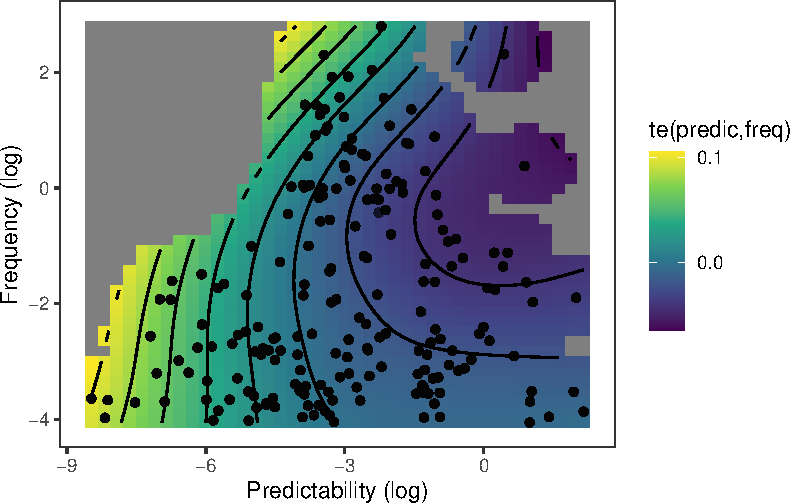
\includegraphics[width=0.8\linewidth,height=\textheight,keepaspectratio]{Chapters/Recognizability/Write-up/quarto-writeup_files/figure-pdf/fig-gam2dplot1-1.pdf}

}

\end{figure}%

\begin{figure}[htbp]

\caption{\label{fig-gam2dplot2}Plot of the interaction effect between
predictability and frequency of our GAM model containing the interaction
between frequency and predictability for phrasal vs nonphrasal verbs.
Brighter colors denote longer reaction times. The left graph is the
predicted effect for phrasal verbs (e.g., pick up), the right graph is
the predicted effect for non-phrasal verbs (e.g., walk up).}

\centering{

\pandocbounded{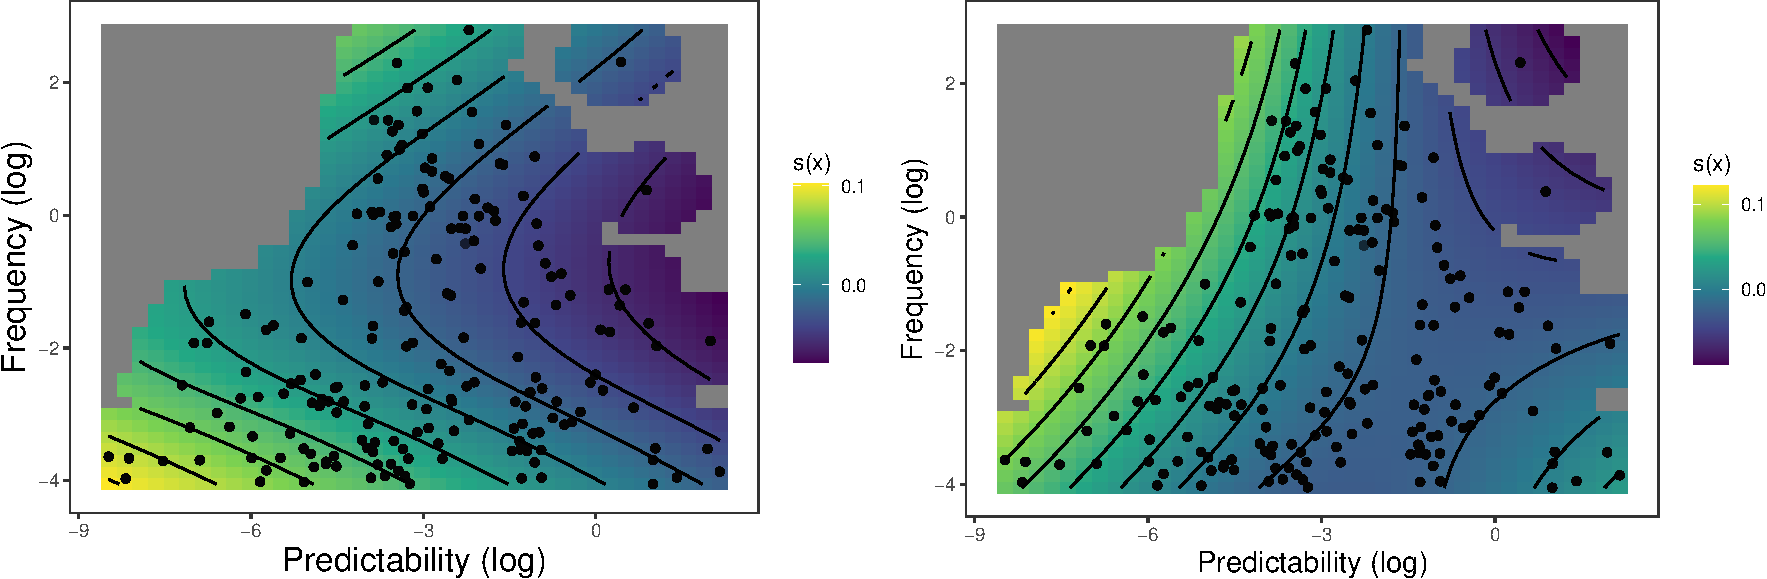
\includegraphics[keepaspectratio]{Chapters/Recognizability/Write-up/quarto-writeup_files/figure-pdf/fig-gam2dplot2-1.pdf}}

}

\end{figure}%

\begin{figure}[htbp]

\caption{\label{fig-gammodelinterplot}Plot of our GAM model's predicted
effect of log(predictability) on recognition time.}

\centering{

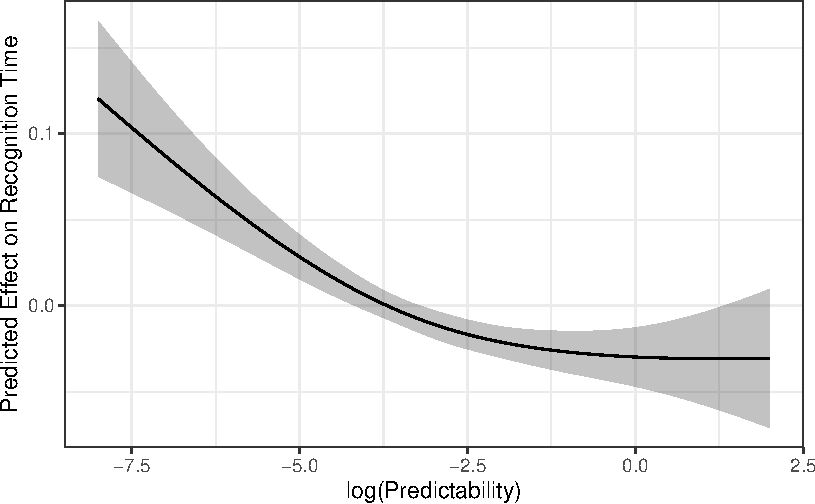
\includegraphics[width=0.8\linewidth,height=\textheight,keepaspectratio]{Chapters/Recognizability/Write-up/quarto-writeup_files/figure-pdf/fig-gammodelinterplot-1.pdf}

}

\end{figure}%

\begin{figure}[htbp]

\caption{\label{fig-FullQuadraticPlot}Visualization of the model results
from Table~\ref{tbl-brmsQuadraticNoInter} for frequency (top) and
predictability (bottom). Frequencies are per million.}

\centering{

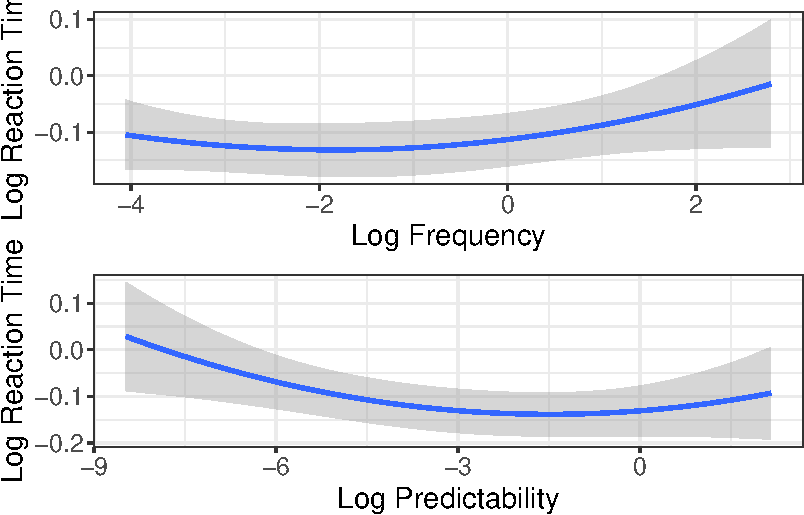
\includegraphics[width=0.8\linewidth,height=\textheight,keepaspectratio]{Chapters/Recognizability/Write-up/quarto-writeup_files/figure-pdf/fig-FullQuadraticPlot-1.pdf}

}

\end{figure}%

\begin{figure}[htbp]

\caption{\label{fig-posteriorplotFullQuadratic}Plot of the posterior
distribution for the beta value of each fixed-effect in our Bayesian
quadratic regression model. The y-axis contains the different
fixed-effects and the x-axis contains the posterior distribution of beta
values for the corresponding fixed-effect.}

\centering{

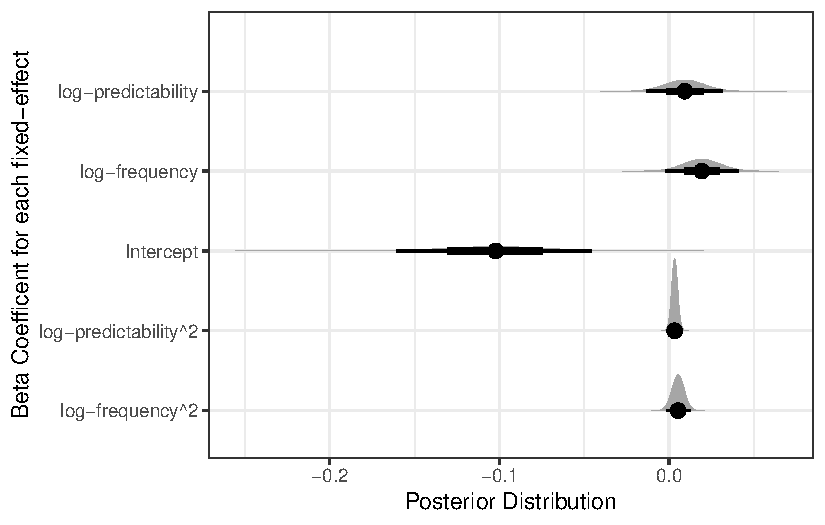
\includegraphics[width=0.8\linewidth,height=\textheight,keepaspectratio]{Chapters/Recognizability/Write-up/quarto-writeup_files/figure-pdf/fig-posteriorplotFullQuadratic-1.pdf}

}

\end{figure}%

\section{Discussion}\label{discussion-4}

The present study examined the effects of frequency and predictability
on the recognizability of the particle \emph{up} in English phrasal
verbs. We found a U-shaped effect for both frequency and predictability
on recognizability: as frequency and predictability increased, people
were faster at recognizing \emph{up}, until reaching the highest
frequency/most predictable items, where people were slower.
Additionally, we also found no meaningful differences between phrasal
verbs (e.g., \emph{pick up}) and non-phrasal verbs (e.g., \emph{stir
up}), suggesting that this slowdown is due to statistical properties of
the language as opposed to syntactic properties.

There are three possible accounts for the slowdown we see for the
highest frequency or predictability items. First, it's possible that
people are attending less to \emph{up} or even skipping it in
high-frequency and high-predictability phrases. This account, unlike the
other accounts that we'll discuss, does not explicitly require the
high-frequency and high-predictability phrases to be stored. Instead,
the listener may be able to process the meaning of the phrase fast
enough that they don't need to wait to hear the entire phrase. For
example, it's possible that for high-frequency and high-predictability
items, when accessing the first word, e.g., \emph{pick}, the listener
accesses the representation of the entire phrase --- either a holistic
representation or a compositional representation --- immediately, before
even hearing \emph{up}. The listener can then continue to process the
next words (skipping over \emph{up}). Since the task is to respond when
they hear \emph{up}, the delay in reaction time may be because they're
not accessing the phonological representation of \emph{up}. Instead,
they may access the semantic representation of the phrase without
initially accessing the phonological representation of \emph{up} and go
on to recover the phonological representation from the semantic
representation of the phrase, causing a delay in recognition time.
Indeed, this possibility was suggested by Healy
(\citeproc{ref-healyDetectionErrorsWord1976}{1976}), who suggested that
in reading once people process the meaning of a word, they move on to
the next word regardless of whether they have processed each individual
letter. This account doesn't explicitly require \emph{pick up} to be
stored holistically since a listener could hear \emph{pick}, predict
\emph{up}, and compose the meaning \emph{pick up} despite having not
heard \emph{up}. However, it also isn't incompatible with a storage
account, since the listener might hear \emph{pick,} predict \emph{up},
and then accesses a stored holistic representation of \emph{pick up}. In
other words, if listeners are attending less to \emph{up}, then it's
unclear whether the listeners are accessing a representation formed by a
compositional process (i.e., accessing \emph{pick,} predicting
\emph{up,} and composing \emph{pick up}) or simply retrieving a stored
form from memory (accessing a holistic representation \emph{pick up}).

The next two accounts all require the high-frequency and
high-predictability items to be stored holistically, but vary with
respect to whether the holistically stored representations retain their
internal structure.

It is possible that the slowdown for the high-frequency and
high-predictability items is due to competition between an additional
representation. This competition can either be between a holistic
representation that has internal structure and a compositional
representation, or between a holistic representation that does not have
internal structure and the compositional representation. Compositional
representation here refers to a representation that is formed by
accessing individual forms (e.g., \emph{pick} and \emph{up}) and
combining them via some generative process. High-frequency and
high-predictability items may develop a holistic representation separate
from the compositional representation and this additional representation
may compete with the compositional representation causing the slowdown.
This account doesn't necessarily need to involve a loss of internal
structure because simply having an additional representation to compete
with can result in a slowdown, however it also not incompatible with an
account where the holistic representation has lost some of its internal
structure. These two possibilities both account for the slowdown at the
highest frequency and highest predictability items.

To break it down further, there is a good deal of evidence that
different mental representations compete for recognition
(\citeproc{ref-oppenheimLexicalCompetitionDemand2019}{Oppenheim \&
Balatsou, 2019}; c.f.
\citeproc{ref-staubInfluenceClozeProbability2015}{Staub et al., 2015}).
A representation is selected once it receives sufficiently more
activation than its competitors
(\citeproc{ref-mcclellandInteractiveActivationModel1981}{McClelland \&
Rumelhart, 1981}). For example, in picture-naming tasks in which
participants are tasked with naming a picture while confronted with a
distractor word, participants are generally slower to produce the
intended word when the distractor word is semantically related to the
picture
(\citeproc{ref-mcclellandInteractiveActivationModel1981}{McClelland \&
Rumelhart, 1981};
\citeproc{ref-schriefersExploringTimeCourse1990}{Schriefers et al.,
1990};
\citeproc{ref-starreveldSemanticInterferenceOrthographic1995}{Starreveld
\& La Heij, 1995}). This effect is not restricted to production as we
see similar competition effects in comprehension as well. For example,
Magnuson et al.
(\citeproc{ref-magnusonDynamicsLexicalCompetition2007}{2007}) examined
the role of competition in word recognition using a visual world
paradigm, where participants saw words on a screen and were instructed
to select the word that they heard. To measure word-recognition, an
eye-tracker was used to track pupil fixations. In each of the trials
there was a single distractor image. They found that words with low
cohort density (i.e., words that have fewer phonological competitors)
showed a larger proportion of target to nontarget fixations. That is,
participants looked the distractor image less relative to the target
word when the word had fewer competitors. Given the inhibitory effects
of competition, it is possible that the delay in reaction time for
\emph{up} in high-frequency and predictability phrases may be a
consequence of an additional representation competing with the
compositional representation. However, there is also evidence that
competition has no effect on comprehension
(\citeproc{ref-staubInfluenceClozeProbability2015}{Staub et al., 2015}).
Using reaction time data from a cloze completion task, Staub et al.
(\citeproc{ref-staubInfluenceClozeProbability2015}{2015}) demonstrated
that a RACE model with neither facilitation nor inhibition between
competitors can account for the data. Thus the evidence for competition
effects in comprehension is mixed. Note that this account is agnostic
about whether the holistic representation has lost its internal
structure or not: simply having an additional representation to compete
with can cause the slowdown.

Lastly it is possible that rather than being driven by competition,
listeners are simply accessing a holistically stored representation of
the phrase that lacks internal structure. This interpretation seems
quite likely given that we see a U-shaped effect in both phrasal (e.g.,
\emph{pick up}) and non-phrasal verbs (e.g., \emph{stir up}). Phrasal
verbs have a syntactic alternation that may lead to all of them being
stored, regardless of whether they are frequent/predictable or not. For
example, In a corpus study, Hampe
(\citeproc{ref-hampeTransitivePhrasalVerbs2012}{2012}) argued that
\emph{Verb-Object-Particle} (e.g., \emph{pick the ball up})
constructions and \emph{Verb-Particle-Object} (e.g., \emph{pick up the
ball}) constructions are two distinct constructions,\footnote{However,
  the same study also makes the claim that these templates are different
  from more lexically specific constructions, thus it is unclear in what
  ways these templates may pattern similarly to holistically stored
  lexical items.} as opposed to being two alternative realizations of a
single constructions. In contrast, non-phrasal verbs can be generated
through compositional knowledge (e.g., \emph{walk up}). This suggests
that phrasal verbs may be stored holistically regardless of
frequency/predictability, while non-phrasal verbs may be generated
compositionally unless they are frequent or predictable enough. If the
increase in reaction time is simply due to competition between the
holistically stored representation and the individual word-level
representations, then if all phrasal verbs are stored we would expect
all of the phrasal verbs to be recognized more slowly. This is because
all of the phrasal verbs, regardless of frequency, would have an
additional representation that would compete for activation. However, we
only see a slowdown for the most frequent or most predictable phrases,
suggesting that storage alone isn't driving the effect. Instead, it is
the combination of storage and usage that leads to loss of internal
representation.

One explanation for why high-frequency and high-predictability items may
not have an intact internal representation is that the internal
structure for those items may never have been learned to begin with.
Children are experts at statistical learning and use transitional
probabilities to divide the continuous speech stream
(\citeproc{ref-saffranStatisticalLearning8MonthOld1996}{Saffran et al.,
1996}). High-predictability phrases in the present study, by definition,
have higher transitional probabilities between words. Thus if children
are relying on transitional probabilities to separate speech into
individual words, the individual words in the most predictable phrases
may not be separated out of the speech stream initially.

Further, many high-frequency (e.g., \emph{set up}) and
high-predictability (e.g., \emph{conjure up}) phrases have semantically
vague relationships that might make it difficult to split them up on a
semantic basis. It seems plausible then that maybe these phrases weren't
learned as being composed of individual words initially and thus the
internal structure for the holistically stored items may not have been
learned. The example, \emph{trick or treat}, is a prime example of a
phrase that does not seem to have a clear semantic relationship between
the phrase and its component parts.

On the other hand, the internal structure may have been lost over time.
For example, Harmon \& Kapatsinski
(\citeproc{ref-harmonPuttingOldTools2017}{2017}) demonstrated that as
learners repeatedly experience a form with a specific meaning, they
become more likely to use that form to express novel meanings in
production (resulting in semantic extension). It is possible that this
accessibility effect similarly drives a loss of internal structure: As a
phrase becomes more semantically extended, the internal structure may be
lost over time. That is, as a phrase such as \emph{pick up} becomes
extended to express novel meanings such as \emph{continue} (``Let's pick
up from where we last left off''), the relationship between the phrase
and its internal pieces (e.g., the relationship between \emph{pick up}
and the individual words \emph{pick} and \emph{up}) becomes less
transparent, and the learner may slowly unlearn this relationship as it
becomes less useful.

In summary, our results suggest that both frequency and predictability
may drive the holistic storage of phrasal verbs, and these holistically
stored items may compete with their component parts during lexical
access. However, future work is still needed to confirm whether the
slowdown for the highest frequency and highest predictability items is
indeed due to a stored holistic representation or if it's due to
shallower attention mechanisms.

\bookmarksetup{startatroot}

\chapter{Emergent Ordering Preferences in Large Language
Models}\label{emergent-ordering-preferences-in-large-language-models}

\section{Introduction}\label{introduction-3}

Large language models have stormed the media in the last few years,
becoming a popular topic in the scientific literature. Their rise to
fame has brought with them many heated debates regarding whether large
language models constitute human-like models of language or whether
their behavior is completely different from humans
(\citeproc{ref-benderDangersStochasticParrots2021}{Bender et al., 2021};
\citeproc{ref-bender2020climbingnlumeaning}{Bender \& Koller, 2020};
\citeproc{ref-piantadosiChapterModernLanguage}{Piantadosi, 2023};
\citeproc{ref-piantadosiMeaningReferenceLarge2022}{Piantadosi \& Hill,
2022}). For example, there has been an ongoing debate about whether
large language models learn any knowledge about the meaning of words.
Bender \& Koller (\citeproc{ref-bender2020climbingnlumeaning}{2020}) has
argued that large language models, which are only trained on the form,
have no way of learning anything about meaning. They pointed out that
large language models do not have the rich information that humans
receive, such as the referent of the form. However, Piantadosi \& Hill
(\citeproc{ref-piantadosiMeaningReferenceLarge2022}{2022}) rebutted this
claim by arguing that co-occurrence statistics can be extremely
informative about a word's meaning. For example, they argued that many
words, such as ``justice'', contain no clear referent and instead have
to be learned by humans based on the context that they occur in. It
seems plausible that large language models could learn at least some
information about the meaning of words in a similar manner.

Other debates have centered around the tradeoff between computation and
storage: how much are these models simply reproducing from their
training data vs how much of their productions are novel utterances
using learned linguistic patterns? On one hand, there is no doubt that
large language models store and reproduce large chunks of language. In
fact, OpenAI is even being sued by \emph{The New York Times} for
allegedly reproducing entire articles verbatim.\footnote{\url{https://nytco-assets.nytimes.com/2023/12/NYT_Complaint_Dec2023.pdf}}
This sentiment -- that large language models are nothing but glorified
copy cats -- has been echoed by several other prominent linguists
(\citeproc{ref-benderDangersStochasticParrots2021}{Bender et al., 2021};
\citeproc{ref-bender2020climbingnlumeaning}{Bender \& Koller, 2020};
c.f., \citeproc{ref-piantadosiMeaningReferenceLarge2022}{Piantadosi \&
Hill, 2022}).

Specifically, proponents of the ``LLMs as copy cats'' argument have
pointed out that large language models are trained on an inconceivably
large amount of data. For example, the OLMo models were trained on
trillions of tokens
(\citeproc{ref-groeneveldOLMoAcceleratingScience2024}{Groeneveld et al.,
2024}).\footnote{This is magnitudes larger than the 350 million words
  that the average college-aged speaker has seen in their lifetime
  (\citeproc{ref-levyProcessingExtraposedStructures2012}{Levy et al.,
  2012}).} As such, it is difficult to determine how much of the text
generated by an LLM is truly novel, and how much is simply reproduced
from its training data. This is further complicated by the fact that
training data for LLMs is typically either not publicly available, or so
huge that it's incredibly difficult to work with. On the other hand, it
is clear that large language models are learning at least some
linguistic patterns. For example, McCoy et al.
(\citeproc{ref-mccoyHowMuchLanguage2023}{2023}) demonstrated that GPT-2
is able to generate well-formed novel words as well as well-formed novel
syntactic structures, despite copying extensively.

These debates, however, have been highly theoretical and speculative and
very few empirical studies have been done to actually investigate these
questions (c.f., \citeproc{ref-lasriSubjectVerbAgreement2022}{Lasri et
al., 2022};
\citeproc{ref-lebrun2022evaluatingdistributionaldistortion}{LeBrun et
al., 2022}; \citeproc{ref-mccoyHowMuchLanguage2023}{McCoy et al., 2023};
\citeproc{ref-panareexplicitbelief}{Pan \& Bergen, 2025}). Thus in the
present paper we address these debates by taking an in-depth look at
large language models' abilities to learn abstract knowledge beyond
simply the statistics of individual tokens. Specifically we examine the
ordering of novel binomials in English (Noun \emph{and} Noun
constructions, e.g., \emph{cats and dogs}). The nouns in binomials can
be ordered without affecting the meaning of the phrase much (e.g.,
\emph{cats and dogs} vs \emph{dogs and cats}). Despite this, human
preferences for which noun should be placed first vary in strength. For
example, there is a pretty strong preference for \emph{bread and butter}
as opposed to \emph{butter and bread}. However, both \emph{computers and
monitors} and \emph{monitors and computers} are natural. Binomials are a
useful test case because there is a great deal of evidence demonstrating
that human ordering preferences are driven by abstract preferences, such
as a preference for more powerful words to be placed first (e.g.,
\emph{god and man} vs \emph{man and god}). Thus by examining binomials
varying in frequency, we can gain insight into whether large language
models are learning abstract preferences and to what degree they learn
similarly to humans.

\subsection{Abstractions in Large Language
Models}\label{abstractions-in-large-language-models}

The evidence for learned abstractions in large language models is
extremely mixed. Investigations into BERT have yielded mixed results for
their ability to learn and apply abstract knowledge
(\citeproc{ref-haleyThisBERTNow2020}{Haley, 2020};
\citeproc{ref-lasriSubjectVerbAgreement2022}{Lasri et al., 2022};
\citeproc{ref-liAssessingCapacityTransformer2023}{Li et al., 2023};
\citeproc{ref-liAreNeuralNetworks2021}{Li \& Wisniewski, 2021}). For
example, Haley (\citeproc{ref-haleyThisBERTNow2020}{2020}) demonstrated
that many of the BERT models are not able to reliably determine the
plurality of novel words. Additionally, Li \& Wisniewski
(\citeproc{ref-liAreNeuralNetworks2021}{2021}) demonstrated that when
tasked with producing the correct tense for a word, BERT tends to rely
on memorization from its training data as opposed to learning the more
general linguistic pattern.

On the other hand, Lasri et al.
(\citeproc{ref-lasriSubjectVerbAgreement2022}{2022}) demonstrated that
BERT can generalize well to novel subject-verb pairs. They tested BERT's
performance on novel sentences along with semantically incoherent but
syntactically sensible sentences (e.g., \emph{colorless green ideas
sleep furiously}) and found that when masking the verb for these
sentences BERT still applies higher probability to the correct
inflection of the verb. Additionally, Li et al.
(\citeproc{ref-liAssessingCapacityTransformer2023}{2023}) demonstrated
that BERT is able to use abstract knowledge to correctly predict
subject-verb and object-past participle agreements in French.

Research using other language models have also yielded similar results.
For example, as mentioned earlier, McCoy et al.
(\citeproc{ref-mccoyHowMuchLanguage2023}{2023}) found that while GPT-2
copies extensively, it also produces both novel words as well as novel
syntactic structures. Additionally Misra \& Mahowald
(\citeproc{ref-misraLanguageModelsLearn2024}{2024}) examined whether a
language model trained on a comparable amount of data as humans can
learn article-adjective-numeral-noun expressions (a beautiful five
days). Specifically, without having a great deal of experience with
them, humans learn that \emph{a beautiful five days} is perfectly
grammatical, but \emph{a blue five days} is not. Misra \& Mahowald
(\citeproc{ref-misraLanguageModelsLearn2024}{2024}) demonstrated that
language models learn this even if they have no AANNs in their training
data. They further demonstrated that they do this by generalizing across
similar constructions, such as \emph{a few days}. Further, Yao et al.
(\citeproc{ref-yaoBothDirectIndirect2025}{2025}) examined whether
language models trained on a comparable amount to humans can learn the
length and animacy preferences that drive dative alternations in humans.
They found that language models can learn these preferences, even
without much experience with the dative alternation. These results
suggest that language models can learn generalizations without a great
amount of data.

Additionally, there's evidence that inducing abstractions facilitates
performance in large language models. For example, Zheng et al.
(\citeproc{ref-zhengTakeStepBack2024}{2023}) used a novel prompting
technique to enable LLMs to use abstractions when reasoning. They found
that LLMs hallucinate less when they implement abstractions in their
reasoning. Similarly, McCoy et al.
(\citeproc{ref-mccoyUniversalLinguisticInductive2020}{2020})
demonstrated that large language models can use abstractions, such as an
abstract preference for certain syllable structures, to learn language
more easily. Their results suggest that inducing abstractions may help
reduce the amount of training that large language models require.

Finally, there is also evidence that transformer models can learn
abstractions from other domains as well. For example, Tartaglini et al.
(\citeproc{ref-tartagliniDeepNeuralNetworks2023}{2023}) examined the
ability of a transformer model in a same-different task (i.e.,
determining if two entities in an image are the same). They found that
some models can reach near perfect accuracy on items they have never
seen before. Since models are learning abstractions in other domains, it
also stands to reason that they may be learning abstractions in
language-related tasks as well.

\subsection{Abstractions in Humans}\label{abstractions-in-humans}

Abstractions have been a part of just about every linguistic theory,
including both generativist and non-generativist theories. This is not
surprising since one of the hallmarks of human language learning is the
ability to produce novel, never-heard-before utterances. In order to do
so, most theories posit that humans leverage their remarkable ability to
learn linguistic patterns beyond simple co-occurrence rates (c.f.,
\citeproc{ref-ambridgeStoredAbstractionsRadical2020}{Ambridge, 2020}).
For example, when presented a novel noun, children are able to
consistently produce the proper plural form of that noun
(\citeproc{ref-berkoChildsLearningEnglish1958}{Berko, 1958}). Similarly,
children are able to leverage similarities across different contexts to
learn a word's general meaning
(\citeproc{ref-yuRapidWordLearning2007}{Yu \& Smith, 2007}).

Abstractions also play a large part in the way that humans linearize
their thoughts into sentences
(\citeproc{ref-morganAbstractKnowledgeDirect2016}{Morgan \& Levy,
2016a}, \citeproc{ref-morgan2024}{2024}). For example, there have been
several studies showing human ordering preferences for binomials are
driven, at least in part, by abstract ordering preferences
(\citeproc{ref-morgan2015}{Morgan \& Levy, 2015},
\citeproc{ref-morganAbstractKnowledgeDirect2016}{2016a},
\citeproc{ref-morgan2024}{2024}). In order to examine this, Morgan \&
Levy (\citeproc{ref-morganAbstractKnowledgeDirect2016}{2016a}) coded a
list of binomials for a variety of semantic, phonological, and metric
constraints that affect human ordering preferences for binomials
(\citeproc{ref-benorChickenEggProbabilistic2006}{Benor \& Levy, 2006}).
They trained a logistic regression model on this corpus to predict the
probability that a binomial will occur in alphabetical order (A and B, a
neutral reference order) as a function of these constraints. They
demonstrated that their logistic regression model performs significantly
better than chance in predicting the ordering of attested binomials from
Siyanova-Chanturia et al.
(\citeproc{ref-siyanova-chanturiaSeeingPhraseTime2011}{2011})'s items
(which the model was not trained on).

The logistic regression model they used combines the various constraints
into a single generative preference constraint that can be used to
examine human ordering preferences. Thus, Morgan \& Levy
(\citeproc{ref-morganAbstractKnowledgeDirect2016}{2016a}) created a
separate list of 42 novel and 42 attested binomials and once again coded
them for the previously-mentioned constraints. They then examined how
human ordering preferences (operationalized as self-paced reading times)
are affected by 1) generative preferences (estimated using the logistic
regression model), 2) relative frequency (for a given binomial, the
proportion of occurrences in alphabetical order to non alphabetical
order), and 3) overall frequency (the total occurrences of the binomial
in alphabetical and nonalphabetical ordering). They found a significant
effect of generative preferences for low-frequency binomials, but not
for high-frequency binomials. This suggests that humans rely on their
compositional knowledge when they have little experience with an item,
but rely on their item-specific experience when they have enough
experience with an item. Interestingly, more recently Morgan \& Levy
(\citeproc{ref-morgan2024}{2024}) also demonstrated that generative
preferences exert a constant effect throughout the frequency spectrum,
affecting even high-frequency binomials (although the effect is weaker
for high-frequency binomials). In other words, even in cases where
humans have experienced a binomial many times, their ordering
preferences aren't driven exclusively by their experience with the
binomial.

Since human ordering preferences deviate from the observed preferences
(i.e., humans aren't simply reproducing binomials in the same order they
they heard them; \citeproc{ref-morgan2024}{Morgan \& Levy, 2024}),
ordering preferences thus present a useful test case for large language
models. If large language models learn representations beyond simply
memorizing the training dataset or superficially reproducing word
co-occurrences, they may learn abstract ordering preferences similar to
humans, and this may be reflected in their binomial ordering
preferences.

\subsection{Present Study}\label{present-study-1}

In the present study we examine whether large language models are simply
copying their input, or whether they are behaving more similarly to
humans and learning abstract linguistics patterns. We use binomials as a
test case because human ordering preferences deviate from the observed
preferences for them. While binomials are a single linguistic
construction, they are well-studied in the linguistics literature and
thus provide us with a strong human baselines that we can compare the
LLM's performance to.

In Experiment 1, we examine whether large language models are sensitive
to ordering preferences for binomials that range from low-frequency to
high-frequency. In Experiment 2, we go more in-depth and explore whether
OLMo-7B (\citeproc{ref-groeneveldOLMoAcceleratingScience2024}{Groeneveld
et al., 2024}) is sensitive to abstract ordering preferences for novel
binomials that the model has never seen before. Finally, in Experiment
3, we examine the same questions at different stages of the model's
training in order to determine how these abstract ordering preferences
emerge as a function of the training.

\section{Experiment 1}\label{experiment-1-1}

\subsection{Methods}\label{methods-5}

\subsubsection{Dataset}\label{dataset}

In order to examine the ordering preferences of binomial constructions
in large language models, we use a corpus of binomials from Morgan \&
Levy (\citeproc{ref-morgan2015}{2015}). The corpus contains 594 binomial
expressions which have been annotated for various phonological,
semantic, and lexical constraints that are known to affect binomial
ordering preferences. The corpus also includes:

\begin{enumerate}
\def\labelenumi{\arabic{enumi}.}
\item
  The estimated generative preferences for each binomial representing
  the ordering preference for the alphabetical ordering (a relatively
  unbiased reference form), estimated from the above constraints
  (independent of frequency). The generative preferences take a value
  between 0 and 1, with 0 being a stronger preference for the
  nonalphabetical form, and 1 being a stronger preference for the
  alphabetical form. The generative constraints were calculated using
  (\citeproc{ref-morgan2015}{Morgan \& Levy, 2015})'s model.
\item
  The observed binomial orderings which are the proportion of binomial
  orderings that are in alphabetical order for a given binomial,
  gathered from the Google \emph{n}-grams corpus
  (\citeproc{ref-linSyntacticAnnotationsGoogle2012}{Lin et al., 2012}).
  The Google \emph{n}-grams corpus is magnitudes larger than the
  language experience of an individual speaker and thus provides
  reliable frequency estimates.
\item
  The overall frequency of a binomial expression (the number of times
  the binomial occurs in either alphabetical or non-alphabetical order).
  Overall frequencies were also obtained from the Google \emph{n}-grams
  corpus (\citeproc{ref-linSyntacticAnnotationsGoogle2012}{Lin et al.,
  2012}).
\end{enumerate}

\subsubsection{Language Model
Predictions}\label{language-model-predictions}

In order to derive predictions for large language models, we used the
following models from the GPT-2
(\citeproc{ref-radfordLanguageModelsAre2019}{Radford et al., 2019})
family, the Llama-2 (\citeproc{ref-touvronLlama2Open2023}{Touvron et
al., 2023}) family, Llama-3 family
(\hyperref[0]{https://github.com/meta-llama/llama3}), and the OLMo
(\citeproc{ref-groeneveldOLMoAcceleratingScience2024}{Groeneveld et al.,
2024}) family. From smallest to largest in number of parameters: GPT-2
(124M paramters), OLMo 1B (1B parameters), GPT-2 XL (1.5B parameters),
Llama-2 7B (7B parameters), OLMo 7B (7B parameters), Llama-3 8B (8B
parameters), Llama-2 13B (13B parameters), and Llama-3 70B (70B
parameters). For each model, we calculated the ordering preferences of
the alphabetical form for each binomial in the dataset. The predicted
probability of the alphabetical form was calculated as the product of
the model's predicted probability of each word in the binomial. In order
to accurately calculate the probability of the first word in the
binomial, each binomial was prepended with the prefix ``Next item:''.
This is necessary because the large language models each provide the
predicted probability of the next word given the current word, so in
order to get the probability of the first word in the binomial, it must
occur after some other token. Following this, the probability of the
alphabetical form, \emph{A and B} is:

\[
\begin{aligned}
    P_{alphabetical} & = P(A|Next\:item: )\\
      & \times P(and|Next\:item: A)\\
      & \times P(B|Next\:item: A\: and)
\end{aligned}
\] \noindent where \emph{A} is the alphabetically first word in the
binomial and \emph{B} is the other word. Additionally, the probability
of the nonalphabetical form, \emph{B and A} is:

\[
\begin{aligned}
    P_{nonalphabetical} & = P(B|Next\:item: )\\
      & \times P(and|Next\:item: B)\\
      & \times P(A|Next\:item: B\: and)
\end{aligned}
\]

Finally, to get an overall ordering preference for the alphabetical
form, we calculated the (log) odds ratio of the probability of the
alphabetical form to the probability of the nonalphabetical form:

\[
LogOdds(AandB) = log(\frac{P_{alphabetical}}{P_{nonalphabetical}})
\]

\subsubsection{Analysis}\label{analysis-2}

The data was analyzed using Bayesian linear regression models,
implemented in \emph{brms}
(\citeproc{ref-burknerBrmsPackageBayesian2017}{Bürkner, 2017}) with
weak, uninformative priors.\footnote{For complete details regarding the
  LM predictions and our analyses, refer to the following link:
  \url{https://github.com/znhoughton/dissertation_writeup/tree/master/Chapters/LLM\%20Ordering\%20Prefs/Scripts}}
For each model, the dependent variable was the log odds of the
alphabetical form to the nonalphabetical form. The fixed-effects were
abstract ordering preference (represented as \emph{AbsPref} below),
observed preference (\emph{ObservedPref}), overall frequency
(\emph{Freq}), an interaction between overall frequency and abstract
ordering preference (\emph{Freq:AbsPref}), and an interaction between
overall frequency and observed preference (\emph{Freq:ObservedPref}).
The model equation is presented below:

\begin{equation}\phantomsection\label{eq-model}{
\begin{aligned}
    LogOdds(AandB) & \sim AbsPref \\
      & + ObservedPref\\
      & + Freq\\
      & + Freq:AbsPref\\ 
      & + Freq:ObservedPref
\end{aligned}
}\end{equation}

\noindent Frequency was logged and centered, and abstract ordering
preference and observed preference were centered such that they ranged
from -0.5 to 0.5 (instead of from 0 to 1). Note that since abstract
ordering preference and observed preference are on the same scale, we
can directly draw comparisons between the coefficient estimates for
these fixed-effects in our regression model.

\subsection{Results}\label{results-5}

Our full model results are presented in the appendix
(Table~\ref{tbl-model_results_full}) and visualized in
Figure~\ref{fig-results}. For each model, the figure shows the values
for each of the coefficients from the model in Equation~\ref{eq-model},
representing how strongly each language model relies on observed
preference, abstract ordering preference, overall frequency, the
interaction between abstract ordering preference and overall frequency,
and the interaction between observed preference and overall frequency.

Our results are similar across all the large language models we tested.
Specifically, we find no effect of abstract ordering preferences and no
interaction effect between abstract ordering preference and overall
frequency. We do find an effect of observed preference suggesting that
the models are mostly reproducing the ordering preferences found in
their training. We also find an interaction effect between observed
preference and overall frequency, suggesting that the effect of observed
frequency is stronger for high-frequency items.

\begin{figure}[htbp]

\caption{\label{fig-results}Results for each beta coefficient estimate
from each model. Models are arranged from smallest to largest from left
to right. The x-axis contains each coefficient and the y-axis contains
the predicted beta coefficient of the respective model. Error bars
indicate 95\textbackslash\% credible intervals.}

\centering{

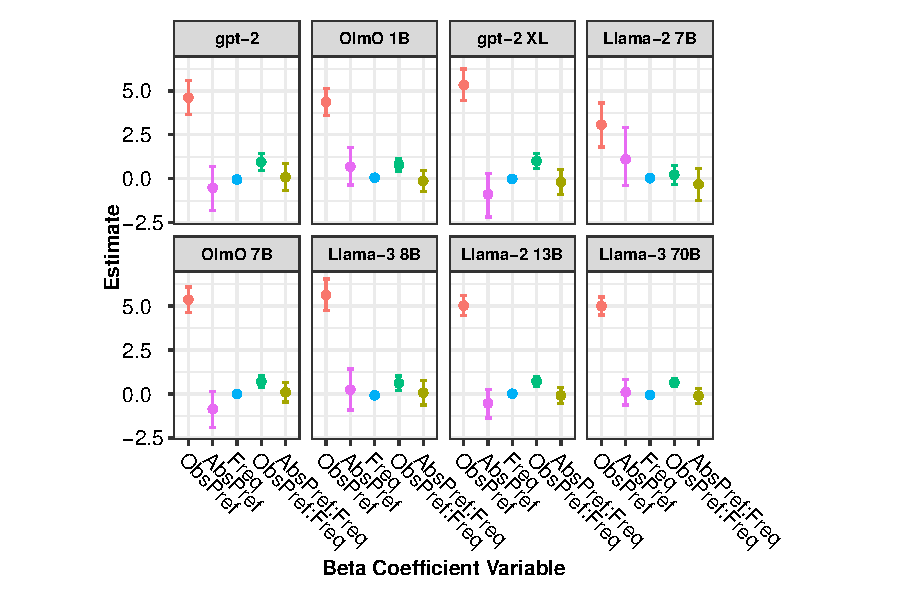
\includegraphics[width=1\linewidth,height=\textheight,keepaspectratio]{Chapters/LLM Ordering Prefs/Figures/full_plot.pdf}

}

\end{figure}%

\subsection{Discussion}\label{discussion-5}

In the present study we examined the extent to which abstract ordering
preferences and observed preferences drive binomial ordering preferences
in large language models. We find that their ordering preferences are
driven primarily by the observed preferences. Further, they rely more on
observed preferences for higher frequency items than lower frequency
items. Finally, they don't seem to be using abstract ordering
preferences at all in their ordering of binomials.

Our results give us insight into the differences between humans and
large language models with respect to the ways in which they trade off
between abstract and observed preferences. For example, our dataset
contains low-frequency binomials (e.g., \emph{alibis and excuses}),
including binomials that a college-age speaker would have heard only
once in their life. Due to their low frequency, humans rely
substantially on abstract ordering preferences to process these lower
frequency items (\citeproc{ref-morgan2024}{Morgan \& Levy, 2024}). This
is not the case, however, for large language models, which rely
exclusively on observed preferences for these items. This is true even
for the smallest models we tested, such as GPT-2. We conclude that,
although large language models can produce human-like language, in the
case of binomials, they accomplish this in a quantitatively different
way than humans do: they rely on observed statistics from the input in
at least some cases when humans would rely on abstract representations.

\section{Experiment 2}\label{experiment-2-1}

In Experiment 1, we demonstrated that large language models don't use
abstract ordering preferences when producing binomials. However, it is
possible that this is because they have experienced the binomials
before, even the low-frequency ones. Thus in Experiment 2 and Experiment
3 we examine whether OLMo-7B is sensitive to abstract ordering
preferences for novel binomials that the model has never seen before. We
also examine the individual constraints that drive abstract ordering
preferences in humans, such as the preference for short words before
long words, to determine whether OLMo is sensitive to the same
constraints in the same way as humans.

Specifically, in Experiment 2, we examine whether OLMo-7B's ordering
preferences are driven by abstract ordering preferences for novel
binomials. In order to do so, we created a list of binomials and
searched the Dolma corpus we created to confirm that they did not occur
in either alphabetical or nonalphabetical ordering. We then coded the
binomials for each of the constraints mentioned earlier. Finally, we
examined whether OLMo-7B shows any preference for one ordering over the
other for each binomial. If OLMo has developed any abstract ordering
preferences, it should show a systematic preference for one ordering
over the other. If it has not, then it should show no preference for one
ordering over the other.

\subsection{Datasets}\label{datasets}

\subsubsection{Dolma}\label{dolma}

For Experiments 2 and 3, we use the dataset described in this section.
In order to examine whether large language models learn preferences
above and beyond simply memorizing co-occurrence rates, we created a
1-grams, 2-grams, and 3-grams corpus of Dolma
(\citeproc{ref-soldainiDolmaOpenCorpus2024}{Soldaini et al., 2024}).
Specifically, we used Dolma version 1\_7 (2.05 trillion tokens), which
was used to train OLMo-7B-v1.7
(\citeproc{ref-groeneveldOLMoAcceleratingScience2024}{Groeneveld et al.,
2024}). Our corpus contains every n-gram (ignoring punctuation and
capitalization) in the Dolma corpus, as well as the number of times that
n-gram appeared.

We then created a list of binomials and searched the corpus to find a
list of binomials that did not occur. We eliminated binomials which
occurred more than zero times in either possible ordering. Thus, OLMo
has had no experience with either ordering of any of our binomials. We
also calculated their unigram and bigram frequencies for each binomial.
Our full list of items comprises 131 binomials and is reproduced in the
appendix section (Section Appendix~\ref{sec-full-list-of-stimuli}).

\subsubsection{Abstract Ordering Preferences
Corpus}\label{abstract-ordering-preferences-corpus}

In order to examine whether large language models are learning
preferences similar to humans, we calculated the abstract ordering
preference value for each of our binomials (following
\citeproc{ref-morganAbstractKnowledgeDirect2016}{Morgan \& Levy,
2016a}). Morgan \& Levy
(\citeproc{ref-morganAbstractKnowledgeDirect2016}{2016a}) demonstrated
that their model's estimated abstract ordering preference value is a
significant predictor of human binomial ordering preferences, even after
accounting for the frequency of each ordering. Abstract ordering
preferences are calculated from a mix of semantic and phonological
properties that human binomial ordering preferences have been shown to
be sensitive to (\citeproc{ref-benorChickenEggProbabilistic2006}{Benor
\& Levy, 2006}). For each of these constraints, a positive value
indicates a preference for the alphabetically first word to be placed
first (a neutral reference order). A negative value indicates a
preference for the nonalphabetical word to be placed first. For example,
a positive value of frequency indicates that the alphabetical word is
more frequent and thus is predicted to be placed first, while a negative
value indicates that the nonalphabetical word is more frequent. The
constraints along with the estimated weights in humans are as follows
(taken from \citeproc{ref-morgan2015}{Morgan \& Levy, 2015}):

\begin{itemize}
\item
  \textbf{Length}: The shorter word should appear first,
  e.g.~\emph{abused and neglected}. In human data, the weight of this
  constraint was estimated to be 0.15.
\item
  \textbf{No Final Stress}: The final syllable of the second word should
  not be stressed, e.g.~\emph{abused and neglected}. In human data, the
  weight of this constraint was estimated to be 0.36.
\item
  \textbf{Lapse:} Avoid unstressed syllables in a row, e.g.~\emph{FARMS
  and HAY-fields} vs \emph{HAY-fields and FARMS.} In human data, the
  weight of this constraint was estimated to be 0.19.
\item
  \textbf{Frequency}: The more frequent word comes first,
  e.g.~\emph{bride and groom}. In human data, the weight of this
  constraint was estimated to be 0.09.
\item
  \textbf{Formal Markedness}: The word with more general meaning or
  broader distribution comes first, e.g.~\emph{boards and two-by-fours}.
  In human data, the weight of this constraint was estimated to be 0.24.
\item
  \textbf{Perceptual Markedness}: Elements that are more closely
  connected to the speaker come first. This constraint encompasses
  Cooper \& Ross (\citeproc{ref-cooper1975worldorder}{1975})`s `Me
  First' constraint and includes numerous subconstraints, e.g.: animates
  precede inanimates; concrete words precede abstract words;
  e.g.~\emph{deer and trees}. In human data, the weight of this
  constraint was estimated to be 0.25.
\item
  \textbf{Power}: The more powerful or culturally prioritized word comes
  first, e.g.~\emph{clergymen and parishioners}. In human data, the
  weight of this constraint was estimated to be 0.26.
\item
  \textbf{Iconic/scalar sequencing}: Elements that exist in sequence
  should be ordered in sequence, e.g.~\emph{achieved and maintained}. In
  human data, the weight of this constraint was estimated to be 1.30.
\item
  \textbf{Cultural Centrality}: The more culturally central or common
  element should come first, e.g.~\emph{oranges and grapefruits}. In
  human data, the weight of this constraint was estimated to be 0.42.
\item
  \textbf{Intensity}: The element with more intensity appear first,
  e.g.~\emph{war and peace}. In human data, the weight of this
  constraint was estimated to be 0.02.
\end{itemize}

\noindent Morgan \& Levy (\citeproc{ref-morgan2015}{2015}) then used a
logistic regression model to combine these constraints into a single
constraint (overall abstract preference) for each binomial.

\subsection{Methods}\label{methods-6}

\subsubsection{Language Model
Predictions}\label{language-model-predictions-1}

We use the same methods as Experiment 1 to obtain language model
predictions for our items.

\subsubsection{Analyses}\label{analyses-2}

We present three Bayesian linear mixed-effects models implemented in
\emph{brms} (\citeproc{ref-burknerBrmsPackageBayesian2017}{Bürkner,
2017}) with weak, uninformative priors. For each of our models, the
intercept represents the grand mean and the coefficient estimates
represent the distance of the effect from the grand mean. Bayesian
statistics don't force us into a binary interpretation of significance,
however we can consider an estimate to be statistically significant if
the credible interval for that estimate excludes zero.

For all three analyses, the dependent variable is LogOdds(AandB), which
was described above. Our dependent variable in the first analysis is the
abstract ordering preference for each binomial (AbsPref). In order to
rule out bigram probabilities as driving the model's preferences, our
second analysis contains the binomial's bigram probabilities (the odds
ratio of product of bigram probabilities of the alphabetical order to
the product of bigram probability of the nonalphabetical order) as well.
Finally, our dependent variables in the third analysis are the
individual constraints that are used to calculate AbsPref. The model
equations are below in Equation~\ref{eq-m1}, Equation~\ref{eq-m2}, and
Equation~\ref{eq-m3}. Note that Formal Markedness and Iconicity were
dropped from the second model because the constraint values were zero
for all of the binomials. Further, our constraints demonstrated a level
of co-linearity. Co-linearity can result in poor model estimates and
inflated credible intervals. In order to deal with this, we dropped the
constraint with the highest variance inflation factor (which turned out
to be the lapse constraint). All other constraints had a variance
inflation factor value below 1.5. We then performed backward model
selection and dropped the predictors whose credible intervals were most
centered around zero until the remaining predictors' credible intervals
were all at least 75\% greater than or less than zero. This resulted in
dropping the no final stress, intense, and percept constraints. We
acknowledge that this approach is quite exploratory and thus
interpretations at the level of the individual constraint must be taken
with a grain of salt.

\begin{equation}\phantomsection\label{eq-m1}{
LogOdds(AandB) \sim AbsPref
}\end{equation}

\begin{equation}\phantomsection\label{eq-m2}{
LogOdds(AandB) ~ AbsPref \cdot BigramProbs
}\end{equation}

\begin{equation}\phantomsection\label{eq-m3}{
LogOdds(AandB) \sim Culture + Power + Freq + Len
}\end{equation}

\subsection{Results}\label{results-6}

The results for the first analysis are presented below in
Table~\ref{tbl-exp1m1}. Our results suggest that there is a main-effect
of abstract ordering preference for OLMo's 7B model. A visualization of
these results can be found below in Figure~\ref{fig-exp1m1}.

\begin{table}

\caption{\label{tbl-exp1m1}Model results examining the effect of AbsPref
on LogOdds(AandB).}

\centering{

\centering\begingroup\fontsize{12}{14}\selectfont

\begin{tabular}{>{\raggedright\arraybackslash}p{12em}rrrrr}
\toprule
\textbf{ } & \textbf{Estimate} & \textbf{Est.Error} & \textbf{Q2.5} & \textbf{Q97.5} & \textbf{\% Samples > 0}\\
\midrule
\textbf{\cellcolor{gray!6}{Intercept}} & \cellcolor{gray!6}{-1.37} & \cellcolor{gray!6}{0.64} & \cellcolor{gray!6}{-2.67} & \cellcolor{gray!6}{-0.22} & \cellcolor{gray!6}{0.7}\\
\textbf{AbsPref} & 2.55 & 1.27 & 0.29 & 5.15 & 98.9\\
\bottomrule
\end{tabular}
\endgroup{}

}

\end{table}%

\begin{figure}[htbp]

\caption{\label{fig-exp1m1}Visualization of the effects of AbsPref on
LogOdds(AandB)}

\centering{

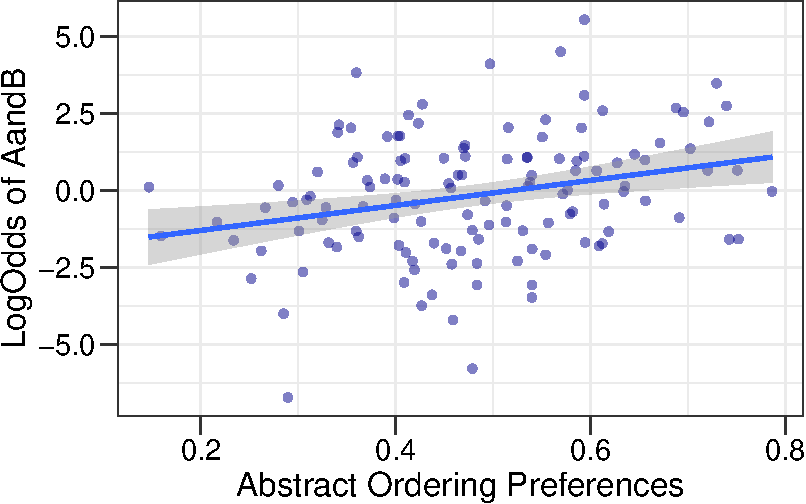
\includegraphics[width=0.8\linewidth,height=\textheight,keepaspectratio]{Chapters/LLM Ordering Prefs/Writeup/writeup-llm-ordering-prefs_files/figure-pdf/fig-exp1m1-1.pdf}

}

\end{figure}%

The results of our second model suggest that the model's ordering
preferences were not driven by bigram probabilities (see
Table~\ref{tbl-exp1bigrams}).

\begin{table}

\caption{\label{tbl-exp1bigrams}Model results examining the effect of
AbsPref and Bigram Probabilities on LogOdds(AandB).}

\centering{

\centering\begingroup\fontsize{12}{14}\selectfont

\begin{tabular}{>{\raggedright\arraybackslash}p{12em}rrrrr}
\toprule
\textbf{ } & \textbf{Estimate} & \textbf{Est.Error} & \textbf{Q2.5} & \textbf{Q97.5} & \textbf{\% Samples > 0}\\
\midrule
\textbf{\cellcolor{gray!6}{Intercept}} & \cellcolor{gray!6}{-1.22} & \cellcolor{gray!6}{0.93} & \cellcolor{gray!6}{-3.30} & \cellcolor{gray!6}{0.29} & \cellcolor{gray!6}{6.80}\\
\textbf{AbsPref} & 2.44 & 1.85 & -0.40 & 6.63 & 94.32\\
\textbf{\cellcolor{gray!6}{BigramProbs}} & \cellcolor{gray!6}{0.50} & \cellcolor{gray!6}{0.75} & \cellcolor{gray!6}{-0.92} & \cellcolor{gray!6}{2.00} & \cellcolor{gray!6}{55.72}\\
\textbf{AbsPref:BigramProbs} & 0.17 & 1.16 & -2.13 & 2.60 & 75.15\\
\bottomrule
\end{tabular}
\endgroup{}

}

\end{table}%

While these results suggest that the large language models' ordering
preferences are sensitive abstract ordering preferences and not bigram
probabilities, it's unclear whether their behavior is similar to humans
on the level of the individual constraints. Thus, in the third analysis
we examined which specific constraints the model is sensitive to, and to
what extent.\footnote{It's also important to consider how many of our
  binomials the constraint even applied to (i.e., how many binomials
  were the constraints non-zero). For the Culture constraint, 62 of our
  131 binomials had a non-zero value. For the Power constraint, 54 were
  non-zero, for the Frequency constraint, all 131 binomials were
  non-zero, and for the Len constraint, 85 were.} For this analysis,
following Houghton et al.
(\citeproc{ref-houghtonTaskdependentConsequencesDisfluency2024}{2024}),
we also present the percentage of posterior samples greater than zero.
The results of this analysis can be found below in
Table~\ref{tbl-exp1m2}.

\begin{table}

\caption{\label{tbl-exp1m2}Model results examining the effect of each
individual constraint on LogOdds(AandB).}

\centering{

\centering\begingroup\fontsize{12}{14}\selectfont

\begin{tabular}{>{\raggedright\arraybackslash}p{12em}rrrrr}
\toprule
\textbf{ } & \textbf{Estimate} & \textbf{Est.Error} & \textbf{Q2.5} & \textbf{Q97.5} & \textbf{\% Samples > 0}\\
\midrule
\textbf{\cellcolor{gray!6}{Intercept}} & \cellcolor{gray!6}{-0.13} & \cellcolor{gray!6}{0.16} & \cellcolor{gray!6}{-0.45} & \cellcolor{gray!6}{0.18} & \cellcolor{gray!6}{20.75}\\
\textbf{Culture} & 0.41 & 0.25 & -0.08 & 0.92 & 94.95\\
\textbf{\cellcolor{gray!6}{Power}} & \cellcolor{gray!6}{0.72} & \cellcolor{gray!6}{0.26} & \cellcolor{gray!6}{0.20} & \cellcolor{gray!6}{1.24} & \cellcolor{gray!6}{99.67}\\
\textbf{Freq} & 0.09 & 0.09 & -0.08 & 0.26 & 85.17\\
\textbf{\cellcolor{gray!6}{Len}} & \cellcolor{gray!6}{-0.21} & \cellcolor{gray!6}{0.13} & \cellcolor{gray!6}{-0.48} & \cellcolor{gray!6}{0.05} & \cellcolor{gray!6}{5.87}\\
\bottomrule
\end{tabular}
\endgroup{}

}

\end{table}%

The model is most sensitive to the Power constraint, however there
appears to be a marginal effect of Culture as well, since nearly 95\% of
the posterior samples are greater than zero despite the credible
interval crossing zero. Surprisingly, there also appears to be a
negative effect of length with a slight preference to place the longer
word first, which is the opposite direction from what we see in humans.
Length is often correlated with frequency, since frequent words tend to
be shorter. As such, we ran a model without frequency to determine
whether the negative effect of length was do to co-linearity with
frequency. However, dropping frequency from the model did not affect the
effect of length. Further, we also ran a model with only length as the
predictor and for that model as well the estimate of length remained
negative.

\subsection{Discussion}\label{discussion-6}

Experiment 2 found that OLMo-7B has learned abstract ordering
preferences even for novel binomials that it has never seen before.
Further, these ordering preferences aren't simply based on the
individual word or bigram frequencies. Specifically, we find a
main-effect of abstract ordering preferences on the model's binomial
ordering preferences. Additionally, we find a strong preference to place
the more powerful word first, a weak preference to place the more
culturally central word first, and a weak preference to place the longer
word first.

These results together suggest that the model is learning abstract
ordering preferences but in a way that is not identical to humans. For
example, while both LLMs and humans show a preference for placing the
more powerful words first and the more culturally central word first,
humans also show a sensitivity to formal markedness, perceptual
markedness, and frequency
(\citeproc{ref-morganAbstractKnowledgeDirect2016}{Morgan \& Levy,
2016a}), which we do not find evidence for in large language models'
binomial ordering preferences. Additionally, humans prefer to place the
shorter word first Morgan \& Levy (\citeproc{ref-morgan2015}{2015}).
However, we find the opposite finding here: large language models prefer
to place the longer word first. One explanation for this is a difference
in terms of the input between humans and large language models. The
length constraint is determined by the number of syllables. While
syllables are salient cues in the audio that humans receive during
learning, it's less clear how salient of a cue they are for large
language models which receive sub-word tokens (which vary in their size,
from being individual orthographic symbols to being entire words.

However, it's unclear how large language models learn these preferences
in the first place. Thus, in Experiment 3 we examine these constraints
at different points in OLMo's training.

\section{Experiment 3}\label{experiment-3-1}

In Experiment 2 we demonstrated that large language models are not
simply copying their training, but are learning some abstract ordering
preferences from their input. However, OLMo makes public various
checkpoints during the model's training, thus allowing us the
opportunity to examine how these preferences arise as a function of the
training. Thus, in Experiment 3 we examine the evolution of these
learned abstract ordering preferences as the model learns over time.

\subsection{Methods}\label{methods-7}

\subsubsection{Language Model
Predictions}\label{language-model-predictions-2}

The language model predictions in Experiment 3 were obtained using the
same procedure as in Experiments 1 and 2. However, instead of
calculating these metrics only for the main model, we calculated them at
various checkpoints. These checkpoints are listed below, in terms of the
steps as well as the number of billions of tokens the model had been
trained on at that checkpoint:

\begin{itemize}
\item
  Step 0, 0B Tokens
\item
  Step 1000, 2B Tokens
\item
  Step 10000, 41B Tokens
\item
  Step 50000, 209B Tokens
\item
  Step 100000, 419B Tokens
\item
  Step 200000, 838B Tokens
\item
  Step 400000, 1677B Tokens
\end{itemize}

\subsubsection{Analysis}\label{analysis-3}

The analyses in Experiment 3 were identical to Experiment 2, however we
ran these analyses for each of the checkpoints listed above.

\subsection{Results}\label{results-7}

Our model estimates for the effect of AbsPref on LogOdds(AandB) at each
checkpoint are presented below in Table~\ref{tbl-exp2m1} and visualized
in Figure~\ref{fig-exp2m1}.

\begin{table}

\caption{\label{tbl-exp2m1}Model results examining the effect of AbsPref
on LogOdds(AandB) for each checkpoint.}

\centering{

\centering\begingroup\fontsize{12}{14}\selectfont

\begin{tabular}{>{\raggedright\arraybackslash}p{12em}rrrrr}
\toprule
\textbf{Number of Tokens} & \textbf{Estimate} & \textbf{Est.Error} & \textbf{Q2.5} & \textbf{Q97.5} & \textbf{\% Samples > 0}\\
\midrule
\textbf{\cellcolor{gray!6}{0B}} & \cellcolor{gray!6}{0.19} & \cellcolor{gray!6}{0.79} & \cellcolor{gray!6}{-1.30} & \cellcolor{gray!6}{1.79} & \cellcolor{gray!6}{59.02}\\
\textbf{2B} & 1.21 & 1.35 & -0.94 & 4.40 & 83.49\\
\textbf{\cellcolor{gray!6}{41B}} & \cellcolor{gray!6}{0.87} & \cellcolor{gray!6}{1.17} & \cellcolor{gray!6}{-1.12} & \cellcolor{gray!6}{3.47} & \cellcolor{gray!6}{77.64}\\
\textbf{209B} & 1.05 & 1.04 & -0.78 & 3.38 & 86.17\\
\textbf{\cellcolor{gray!6}{419B}} & \cellcolor{gray!6}{1.70} & \cellcolor{gray!6}{1.22} & \cellcolor{gray!6}{-0.36} & \cellcolor{gray!6}{4.33} & \cellcolor{gray!6}{94.24}\\
\addlinespace
\textbf{838B} & 1.77 & 1.27 & -0.32 & 4.58 & 94.05\\
\textbf{\cellcolor{gray!6}{1677B}} & \cellcolor{gray!6}{3.86} & \cellcolor{gray!6}{1.52} & \cellcolor{gray!6}{0.95} & \cellcolor{gray!6}{6.82} & \cellcolor{gray!6}{99.88}\\
\bottomrule
\end{tabular}
\endgroup{}

}

\end{table}%

The model results are visualized below in Figure~\ref{fig-exp2m1}.

\begin{figure}[htbp]

\caption{\label{fig-exp2m1}Visualization of the model predictions for
the effect of AbsPref on LogOdds(AandB) for each checkpoint.}

\centering{

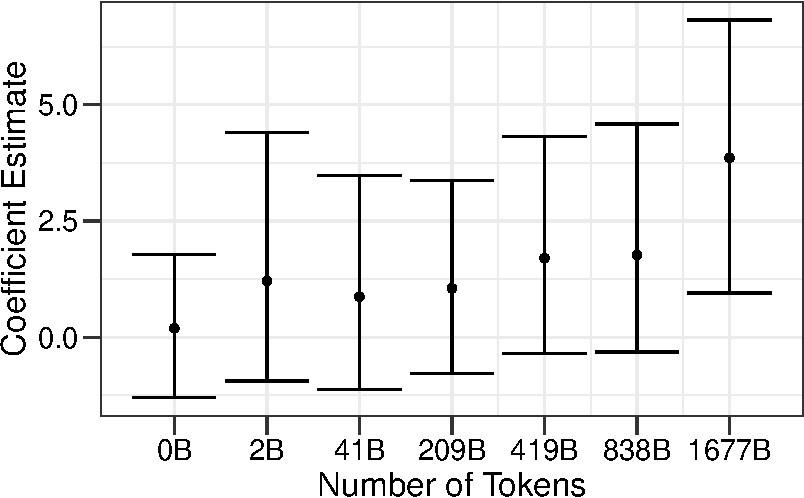
\includegraphics[width=0.7\linewidth,height=\textheight,keepaspectratio]{Chapters/LLM Ordering Prefs/Writeup/writeup-llm-ordering-prefs_files/figure-pdf/fig-exp2m1-1.pdf}

}

\end{figure}%

Our results demonstrate that it takes quite a large number of tokens for
the model to learn the abstract ordering preferences. As
Figure~\ref{fig-exp2m1} demonstrates, the effect of abstract ordering
preference isn't convincing until the model has experienced 1677B
tokens. However, it does appear that the model develops a slight
preference quite rapidly. For example, by 2 billion tokens there appears
to be a very slight (though unconvincing) effect of abstract ordering
preferences on the ordering of binomials.

Similar to Experiment 2, in our second analysis we present a breakdown
of the effects of each individual constraint. In this analysis, however,
we demonstrate the effect of each constraint at each checkpoint. The
full table results can be found in the the appendix section
(Appendix~\ref{sec-individual-constraints-at-each-checkpoint}), but we
present a visualization below in Figure~\ref{fig-exp2m2}.

\begin{figure}[htbp]

\caption{\label{fig-exp2m2}Visualization of the effect of each
constraint on the ordering preference at each checkpoint.}

\centering{

\pandocbounded{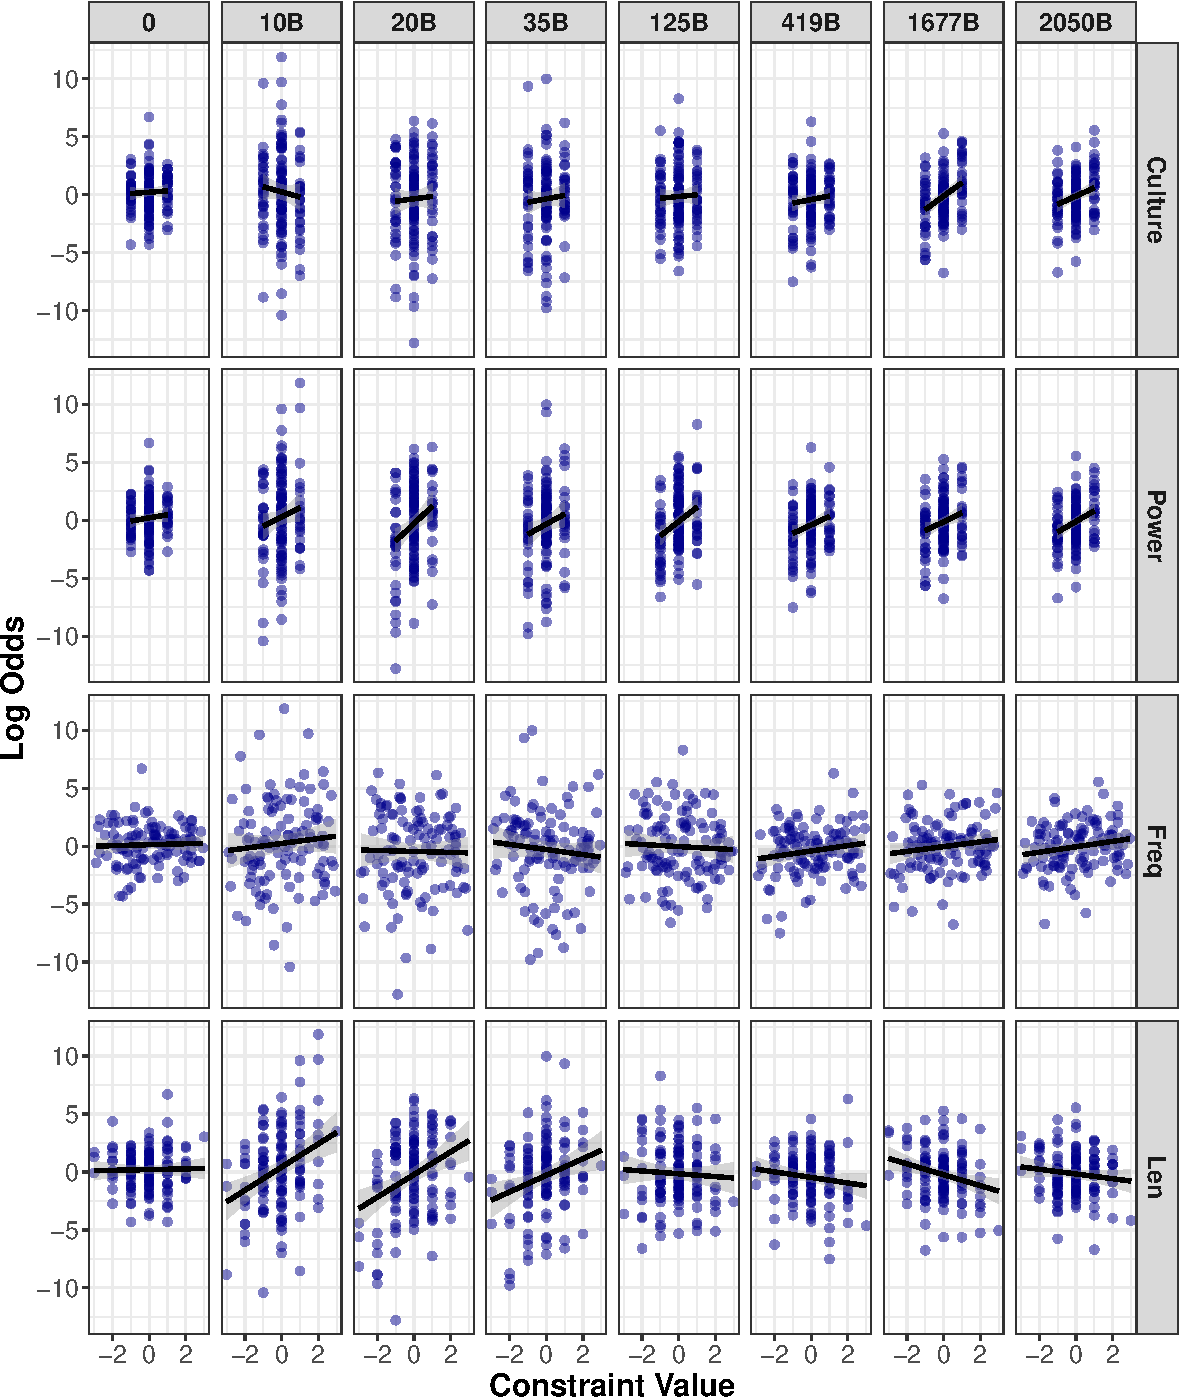
\includegraphics[keepaspectratio]{Chapters/LLM Ordering Prefs/Writeup/writeup-llm-ordering-prefs_files/figure-pdf/fig-exp2m2-1.pdf}}

}

\end{figure}%

Interestingly, it appears that early on the model already shows evidence
of learning human-like preferences. For example, by 10 billion tokens
the model has learned to place more powerful words first and shorter
words first. However, the model seems slower to learn to place more
culturally central words first. Further, as it receives more training
the effect of length undergoes a reversal in direction.

\subsection{Discussion}\label{discussion-7}

Our results demonstrate that OLMo learns ordering preferences early on
for the power, frequency, and length constraints, but is slower to learn
ordering preferences for the culture constraint. Further, the model is
human-like in its predictions for length early on, but as it receives
more training data it learns the opposite length prediction. It is
unclear what exactly is causing this reversal, but it may be a function
of the tokenization differences between human input and large language
models' input.

It is interesting that the model is quick to learn the power constraint,
but slower to learn the culture constraint. Both constraints require a
level of world-knowledge but the model learns which entities are more
powerful relatively quickly, but not which is more culturally central.
One interesting question is whether humans also take longer to learn the
culture constraint, or whether they learn this early on. If children
learn this constraint early on it may suggest differences with respect
to how easily large language models learn world knowledge. On the other
hand, if children also take longer to learn the culture constraint it
may suggest that the power constraint is simply easier to learn.

\section{Conclusion}\label{conclusion-1}

In the present study, we examined the ordering preferences of binomials
in various large language models. We found that for binomials that the
models have experienced, they do not use abstract preferences but
instead reproduce them proportionately to their training data. This is
the case even for low-frequency binomials. Interestingly, for novel
binomials, we found that they do learn and use abstract ordering
preferences.

Additionally, while overall the model does show evidence of having
learned abstract preferences, these preferences are not identical to
human ordering preferences. For example, the model shows a preference
for longer words placed before shorter words, which is the opposite of
what humans prefer.

Further, show that while the effect of abstract ordering preference on a
whole takes a great deal of time (over 1677B tokens to be convincing),
the model seems to learn human-like preferences at the level of some
individual constraints quite early on.

Overall, our results suggest that large language models are not simply
copying their input, but are learning interesting, human-like phenomena
from their training. However, they are not learning identically to
humans, as demonstrated by the opposite direction of the length
preference. Further, while humans rely on abstract preferences even for
binomials that they have encountered before, even high-frequency ones
(\citeproc{ref-morgan2024}{Morgan \& Levy, 2024}), large language models
rely on abstract ordering preferences only for items that they have not
encountered at all. In other words, while large language models are able
to learn abstract ordering preferences, in cases where humans would rely
on these preferences, large language models seem to rely instead on
their experience with the item.

\bookmarksetup{startatroot}

\chapter{Holistic Representations of Binomials in Large Language
Models}\label{holistic-representations-of-binomials-in-large-language-models}

\section{Introduction}\label{introduction-4}

In the last few years large language models have surged in popularity
and have remained in the center of both the media coverage and academic
research. Their surge in popularity has sparked many debates about the
extent to which they constitute an effective model of human language
(e.g., \citeproc{ref-benderDangersStochasticParrots2021}{Bender et al.,
2021}; \citeproc{ref-piantadosiChapterModernLanguage}{Piantadosi, 2023};
\citeproc{ref-piantadosiMeaningReferenceLarge2022}{Piantadosi \& Hill,
2022}). These debates have stemmed from clear differences in terms of
both the training that the models receive as well as the performance of
these models on language processing tasks. For example, common
criticisms include their insanely large training size (sometimes being
trained on upwards of 15 billion tokens), the potentially unrealistic
nature of their tokenization (e.g., Chat GPT tokenizes kite as
{[}\emph{k}, \emph{ite}{]}\footnote{\url{https://tiktokenizer.vercel.app/}}),
and their poor performance on tasks that are trivial to humans (e.g.,
counting the number of \emph{r}'s in \emph{strawberry}\footnote{\url{https://community.openai.com/t/incorrect-count-of-r-characters-in-the-word-strawberry/829618}}).

Many of these debates are centered around the extend to which large
language models are actually learning something abstract from the data
and to what extent they are simply regurgitating their training data.
However, despite a large body of research, the results have been quite
mixed (\citeproc{ref-haleyThisBERTNow2020}{Haley, 2020};
\citeproc{ref-lasriSubjectVerbAgreement2022}{Lasri et al., 2022};
\citeproc{ref-liAssessingCapacityTransformer2023}{Li et al., 2023};
\citeproc{ref-liAreNeuralNetworks2021}{Li \& Wisniewski, 2021};
\citeproc{ref-mccoyHowMuchLanguage2023}{McCoy et al., 2023};
\citeproc{ref-misraLanguageModelsLearn2024}{Misra \& Mahowald, 2024};
\citeproc{ref-yaoBothDirectIndirect2025}{Yao et al., 2025}). For
example, Haley (\citeproc{ref-haleyThisBERTNow2020}{2020}) demonstrated
that many BERT models are not able to reliably determine the correct
plural form for novel words. Similarly, Li \& Wisniewski
(\citeproc{ref-liAreNeuralNetworks2021}{2021}) demonstrated that BERT
tends to rely on memorization from its training data when producing the
correct tense of novel words.

In contrast, recent research has demonstrated BERT's ability to
generalize well to novel subject-verb pairs
(\citeproc{ref-lasriSubjectVerbAgreement2022}{Lasri et al., 2022}) and
to use abstract knowledge to predict object-past participle agreements
in French (\citeproc{ref-liAssessingCapacityTransformer2023}{Li et al.,
2023}). Further, McCoy et al.
(\citeproc{ref-mccoyHowMuchLanguage2023}{2023}) demonstrated that while
GPT-2 copies extensively, it also produces both novel words as well as
novel syntactic structures.

Additionally, in an attempt to address criticism about the unrealistic
size of the training data for large language models, an interesting line
of research has demonstrated that even smaller language models trained
on an amount of data comparable to humans seem to be able to learn
abstract linguistic knowledge from the data
(\citeproc{ref-misraLanguageModelsLearn2024}{Misra \& Mahowald, 2024};
\citeproc{ref-yaoBothDirectIndirect2025}{Yao et al., 2025}). For
example, Misra \& Mahowald
(\citeproc{ref-misraLanguageModelsLearn2024}{2024}) examined whether a
language model trained on a similar amount of data as humans could learn
article-adjective-numeral-noun expressions (AANNs, e.g., \emph{a
beautiful five days}). They found that even after removing AANNs from
the training data, language models are still able to learn which AANNs
are appropriate and which ones are not (e.g., *\emph{a blue five days}).
Additionally, Yao et al.
(\citeproc{ref-yaoBothDirectIndirect2025}{2025}) examined whether a
similar language model can learn the length and animacy preferences for
the dative alternation (give X Y vs give Y to X). They found that a
language model trained on a comparable amount of data as humans is able
to learn these preferences. These results together demonstrate the
ability for language models to learn general knowledge about the
language.

Given the evidence that large language models show evidence of both
learning abstract knowledge as well as copying extensively from their
training data, it's unclear in what contexts they are leveraging their
stored knowledge as opposed to leveraging abstract knowledge of the
language.

\subsection{Stored Representations in
Humans}\label{stored-representations-in-humans}

There's a great deal of evidence that humans store holistically many
multi-morphemic words and multi-word phrases
(\citeproc{ref-bybee2003}{Bybee, 2003};
\citeproc{ref-bybeeEffectUsageDegrees1999}{Bybee \& Scheibman, 1999};
\citeproc{ref-stembergerFrequencyLexicalStorage1986}{Stemberger \&
MacWhinney, 1986},
\citeproc{ref-stembergerAreInflectedForms2004}{2004}). For example,
high-frequency phrases containing \emph{don't} (e.g., \emph{I don't
know}) are more likely to be phonetically reduced than lower frequency
words containing \emph{don't}
(\citeproc{ref-bybeeEffectUsageDegrees1999}{Bybee \& Scheibman, 1999}).
This suggests that higher-frequency phrases are represented holistically
because the phonetic reduction at the phrase-level cannot simply be
attributed to phonetic reduction at the individual word-level.

Additionally, there is also evidence from the psycholinguistics
literature that high-frequency multi-word phrases are stored
holistically (\citeproc{ref-morgan2015}{Morgan \& Levy, 2015},
\citeproc{ref-morganAbstractKnowledgeDirect2016}{2016a},
\citeproc{ref-morganFrequencydependentRegularizationIterated2016a}{2016b},
\citeproc{ref-morgan2024}{2024};
\citeproc{ref-odonnellProductivityReuseLanguage2016}{O'Donnell, 2016};
\citeproc{ref-siyanova-chanturiaSeeingPhraseTime2011}{Siyanova-Chanturia
et al., 2011}). For example, Siyanova-Chanturia et al.
(\citeproc{ref-siyanova-chanturiaSeeingPhraseTime2011}{2011})
demonstrated that binomials (e.g., \emph{bread and butter}) are read
faster in their frequent ordering (\emph{bread and butter}) than in
their infrequent ordering (\emph{butter and bread}). This suggests that
reading times for multi-word phrases can't be reduced to the reading
times of the individual words. However, it is possible that these faster
reading times are driven by knowledge of generative preferences, such as
a preference for short words before long words. Thus to investigate
this, Morgan \& Levy
(\citeproc{ref-morganAbstractKnowledgeDirect2016}{2016a}) examined
whether human reading times for binomials are driven by generative
preferences (e.g., a preference for more culturally central words first)
or by experience with the binomial. Specifically, they examined whether
human ordering preferences were driven simply by the relative frequency
of the binomial. For example, \emph{bread and butter} is vastly
preferred over \emph{butter and bread}. Is this driven by the fact that
\emph{bread and butter} is more frequent than \emph{butter and bread} or
driven by more abstract constraints, such as a preference for short
words first? Interestingly, they found that high-frequency binomial
ordering preferences are driven primarily by experience (i.e., the more
frequent ordering is preferred) while low-frequency binomial ordering
preferences are driven primarily by generative preferences (e.g., a
preference for short words before long words).

Given that humans rely on generative preferences for some binomials and
item-specific preferences for other binomials, binomials present a good
test case for examining this same trade off in large language models.
Specifically, since humans holistically store high-frequency binomials
holistically and compose low-frequency binomials using generative
knowledge, if large language models are learning similarly they may
similarly represent high-frequency binomials systematically differently
from low-frequency binomials.

\subsection{Present Study}\label{present-study-2}

Since humans rely more on abstract knowledge for lower frequency items
and rely more on their experience for high-frequency binomials
(\citeproc{ref-morgan2024}{Morgan \& Levy, 2024}), a natural consequence
of this is that they have learned separate representations for
high-frequency binomials (i.e., holistic storage). If large language
models are learning similarly to humans, they may also learn separate
representations for high-frequency binomials but not for lower-frequency
binomials.

The present study addresses this question by examining the semantic
representations of binomials varying in relative frequency (the
proportion of occurrences in one ordering to the other ordering) and
overall frequency (the overall frequency of the binomial, regardless of
ordering). We examine the embeddings for both ordering of binomials in a
sentence context, as well as examine the embeddings for a compositional
form of the binomial (which we will elaborate on in the methods
section). We hypothesize that the representations of the more frequent
form (higher relative frequency form) for binomials with a high overall
frequency may diverge more from the compositional representation than
the less frequent ordering (lower relative frequency form) does for the
same binomial. That is, for high-frequency binomials, the representation
for the more frequent ordering may be more different from the
compositional representation than the less-frequent ordering is.
However, for lower-frequency binomials, large language models may not
learn different representations for the different orderings of the same
form, regardless of the relative frequency.

In Experiment 1, we examine the representations of different binomials
across different large language models and in Experiment 2 we examine
the timecourse of these representations across each hidden layer in
OLMo's 1B model
(\citeproc{ref-groeneveldOLMoAcceleratingScience2024}{Groeneveld et al.,
2024}).

\section{Experiment 1}\label{experiment-1-2}

In Experiment 1 we examine the representations of binomials for GPT-2,
GPT-2 XL (\citeproc{ref-radfordLanguageModelsAre2019}{Radford et al.,
2019}), OLMo-1B, OLMo-7B
(\citeproc{ref-groeneveldOLMoAcceleratingScience2024}{Groeneveld et al.,
2024}), and Llama2-7B (\citeproc{ref-touvronLlama2Open2023}{Touvron et
al., 2023}). We examine the representations for different binomials in
sentence contexts as well as the compositional representations of those
same binomials. We explain these metrics in detail below.

\subsection{Methods}\label{methods-8}

\subsubsection{Dataset}\label{dataset-1}

Our dataset consists of 784 sentences containing binomials. The
sentences have been annotated for both relative frequency and overall
frequency. Relative frequency is operationalized as the proportion of
occurrences in alphabetical order (a neutral reference order) to
occurrences in nonalphabetical order. Overall frequency is
operationalized as the count of \emph{A and B} plus the count of \emph{B
and A}. Counts for both measures were obtained using the Google
\emph{n-}grams corpus
(\citeproc{ref-linSyntacticAnnotationsGoogle2012}{Lin et al., 2012}).

\subsubsection{Semantic Embeddings}\label{semantic-embeddings}

In order to examine the semantic compositionality of binomials, we
examined the semantic embeddings of five different large language
models: GPT-2, GPT-2 XL
(\citeproc{ref-radfordLanguageModelsAre2019}{Radford et al., 2019}),
Llama-2 7B (\citeproc{ref-touvronLlama2Open2023}{Touvron et al., 2023}),
OLMo 1B and OLMo 7B
(\citeproc{ref-groeneveldOLMoAcceleratingScience2024}{Groeneveld et al.,
2024}).

For each LLM we examined the semantic embeddings of the binomials in a
sentence context. We accomplished this by passing the sentence through
each large language model and extracting the second-to-last hidden layer
for each of the words in the binomial. We did this once for the
alphabetical ordering of the binomial (A and B) and once for the
non-alphabetical ordering of the binomial (B and A). Since LLMs generate
an embedding for each word, we computed the mean of these embeddings to
represent the semantic embedding of the entire binomial in a sentence
context (hereafter referred to as holistic embeddings). Next, we
obtained the embedding for each word in the binomial individually,
outside of a sentence context. We then computed the mean of these
embeddings to represent the semantic embedding of the compositional form
of the binomial (hereafter referred to as the compositional embeddings).

We then measured the cosine similarity between the holistic embeddings
and the compositional embeddings for the alphabetical and
nonalphabetical ordering of each binomial. This is presented
mathematically in Equation~\ref{eq-cosalpha} and
Equation~\ref{eq-cosnonalpha}, where \(cos_\alpha\) is the cosine
similarity between the holistic embeddings of the alphabetical order of
the binomial and the compositional embeddings, \(cos_{\neg\alpha}\) is
the cosine similarity between the embeddings of the nonalphabetical
order of the binomial and the compositional embeddings, \(h_\alpha\) and
\(h_{\neg\alpha}\) are the holistic embeddings of the binomial in
alphabetical and nonalphabetical ordering respectively (in a sentence
context), and \(c\) is the compositional embeddings. Since \(c\)
represents the mean of the embeddings for each word in the binomial out
of context, order does not matter. Cosine similarity ranges from -1 to 1
where 1 indicates two extremely similar vectors and -1 indicates two
extremely dissimilar vectors.

\begin{equation}\phantomsection\label{eq-cosalpha}{
\cos \alpha = \frac{h_\alpha \cdot c}{\left\lVert h_\alpha \right\rVert \left\lVert c \right\rVert}
}\end{equation}

\begin{equation}\phantomsection\label{eq-cosnonalpha}{
\cos \neg\alpha = \frac{h_{\neg\alpha} \cdot c}{\left\lVert h_{\neg\alpha}\right\rVert \left\lVert c \right\rVert}
}\end{equation}

For each binomial, we then calculated \(LogCosSim\) which is the logged
quotient of \(cos_\alpha\) and \(cos_{\neg\alpha}\)
(Equation~\ref{eq-cossim}). A larger positive value indicates a greater
degree of similarity between the holistic embeddings of the alphabetical
order and the compositional embeddings (i.e., the similarity between the
holistic embeddings of the alphabetical ordering and the compositional
embeddings is greater than the similarity between the holistic
embeddings of the nonalphabetical ordering and the compositional
embeddings) and a larger negative value represents the opposite.

\begin{equation}\phantomsection\label{eq-cossim}{
LogCosSim = log(\frac{cos_\alpha}{cos_{\neg\alpha}})
}\end{equation}

\subsubsection{Analysis}\label{analysis-4}

We used a Bayesian mixed-effects model to examine how the semantic
similarity between the holistic embeddings and the compositional
embeddings trade off as a function of relative and overall
frequency.\footnote{For more details regarding our analysis, refer to
  the following link:
  \url{https://github.com/znhoughton/dissertation_writeup/tree/master/Chapters/LLM\%20Storage}}
Specifically, we modeled \(LogCosSim\) as a function of overall
frequency, which was centered and logged, \(RelFreq\) which ranged from
-0.5 to 0.5 (with 0.5 representing a binomial that appears only in the
alphabetical form, and -0.5 representing a binomial that appears only in
the nonalphabetical form), and their interaction. Our model is presented
below in Equation~\ref{eq-m4}. We used weak, uninformative priors.

\begin{equation}\phantomsection\label{eq-m4}{
LogCosSim \sim OverallFreq*RelFreq
}\end{equation}

\subsection{Results}\label{results-8}

Our results for each model are presented in Table~\ref{tbl-modelsall}
and visualized in Figure~\ref{fig-modelsall}. Following
(\citeproc{ref-houghtonTaskdependentConsequencesDisfluency2024}{Houghton
et al., 2024}) we also report the percentage of posterior samples
greater than zero. Since we are using Bayesian mixed-effects models, we
are not forced into a binary of significant or non-significant. By
reporting the percentage of posterior samples greater than zero, we
present a more nuanced picture of our results.

\begin{table}

\caption{\label{tbl-modelsall}Bayesian linear mixed-effects model
results of each model}

\centering{

\centering\begingroup\fontsize{12}{14}\selectfont

\begin{tabular}{>{\raggedright\arraybackslash}p{12em}rrrrr}
\toprule
\textbf{ } & \textbf{Estimate} & \textbf{Est.Error} & \textbf{Q2.5} & \textbf{Q97.5} & \textbf{\% Samples > 0}\\
\midrule
\addlinespace[0.3em]
\multicolumn{6}{l}{\textbf{GPT-2}}\\
\textbf{\hspace{1em}\cellcolor{gray!6}{Intercept}} & \cellcolor{gray!6}{0.00} & \cellcolor{gray!6}{0.00} & \cellcolor{gray!6}{0.00} & \cellcolor{gray!6}{0.00} & \cellcolor{gray!6}{72.44}\\
\textbf{\hspace{1em}OverallFreq} & 0.00 & 0.00 & 0.00 & 0.00 & 14.22\\
\textbf{\hspace{1em}\cellcolor{gray!6}{RelFreq}} & \cellcolor{gray!6}{-0.04} & \cellcolor{gray!6}{0.01} & \cellcolor{gray!6}{-0.05} & \cellcolor{gray!6}{-0.02} & \cellcolor{gray!6}{0.00}\\
\textbf{\hspace{1em}OverallFreq:RelFreq} & 0.00 & 0.00 & -0.01 & 0.00 & 0.04\\
\addlinespace[0.3em]
\multicolumn{6}{l}{\textbf{GPT-2 XL}}\\
\textbf{\hspace{1em}\cellcolor{gray!6}{Intercept}} & \cellcolor{gray!6}{0.00} & \cellcolor{gray!6}{0.00} & \cellcolor{gray!6}{0.00} & \cellcolor{gray!6}{0.00} & \cellcolor{gray!6}{14.77}\\
\textbf{\hspace{1em}OverallFreq} & 0.00 & 0.00 & 0.00 & 0.00 & 99.67\\
\textbf{\hspace{1em}\cellcolor{gray!6}{RelFreq}} & \cellcolor{gray!6}{0.00} & \cellcolor{gray!6}{0.01} & \cellcolor{gray!6}{-0.01} & \cellcolor{gray!6}{0.01} & \cellcolor{gray!6}{68.45}\\
\textbf{\hspace{1em}OverallFreq:RelFreq} & 0.00 & 0.00 & 0.00 & 0.01 & 97.82\\
\addlinespace[0.3em]
\multicolumn{6}{l}{\textbf{OLMo-1B}}\\
\textbf{\hspace{1em}\cellcolor{gray!6}{Intercept}} & \cellcolor{gray!6}{0.00} & \cellcolor{gray!6}{0.01} & \cellcolor{gray!6}{-0.01} & \cellcolor{gray!6}{0.02} & \cellcolor{gray!6}{56.38}\\
\textbf{\hspace{1em}OverallFreq} & 0.00 & 0.00 & -0.01 & 0.00 & 33.00\\
\textbf{\hspace{1em}\cellcolor{gray!6}{RelFreq}} & \cellcolor{gray!6}{-0.15} & \cellcolor{gray!6}{0.03} & \cellcolor{gray!6}{-0.21} & \cellcolor{gray!6}{-0.10} & \cellcolor{gray!6}{0.00}\\
\textbf{\hspace{1em}OverallFreq:RelFreq} & -0.02 & 0.01 & -0.03 & 0.00 & 0.43\\
\addlinespace[0.3em]
\multicolumn{6}{l}{\textbf{OLMo-7B}}\\
\textbf{\hspace{1em}\cellcolor{gray!6}{Intercept}} & \cellcolor{gray!6}{0.00} & \cellcolor{gray!6}{0.01} & \cellcolor{gray!6}{-0.01} & \cellcolor{gray!6}{0.02} & \cellcolor{gray!6}{55.77}\\
\textbf{\hspace{1em}OverallFreq} & 0.00 & 0.00 & -0.01 & 0.00 & 32.45\\
\textbf{\hspace{1em}\cellcolor{gray!6}{RelFreq}} & \cellcolor{gray!6}{-0.15} & \cellcolor{gray!6}{0.03} & \cellcolor{gray!6}{-0.21} & \cellcolor{gray!6}{-0.09} & \cellcolor{gray!6}{0.00}\\
\textbf{\hspace{1em}OverallFreq:RelFreq} & -0.02 & 0.01 & -0.03 & 0.00 & 0.58\\
\addlinespace[0.3em]
\multicolumn{6}{l}{\textbf{Llama2-7B}}\\
\textbf{\hspace{1em}\cellcolor{gray!6}{Intercept}} & \cellcolor{gray!6}{0.00} & \cellcolor{gray!6}{0.00} & \cellcolor{gray!6}{-0.01} & \cellcolor{gray!6}{0.00} & \cellcolor{gray!6}{9.25}\\
\textbf{\hspace{1em}OverallFreq} & 0.00 & 0.00 & 0.00 & 0.00 & 3.40\\
\textbf{\hspace{1em}\cellcolor{gray!6}{RelFreq}} & \cellcolor{gray!6}{-0.01} & \cellcolor{gray!6}{0.01} & \cellcolor{gray!6}{-0.03} & \cellcolor{gray!6}{0.01} & \cellcolor{gray!6}{8.06}\\
\textbf{\hspace{1em}OverallFreq:RelFreq} & 0.00 & 0.00 & -0.01 & 0.00 & 3.17\\
\bottomrule
\end{tabular}
\endgroup{}

}

\end{table}%

\begin{figure}[htbp]

\caption{\label{fig-modelsall}Visualization of the effects of overall
frequency and relative frequency on the cosine similarity between
embeddings.}

\centering{

\pandocbounded{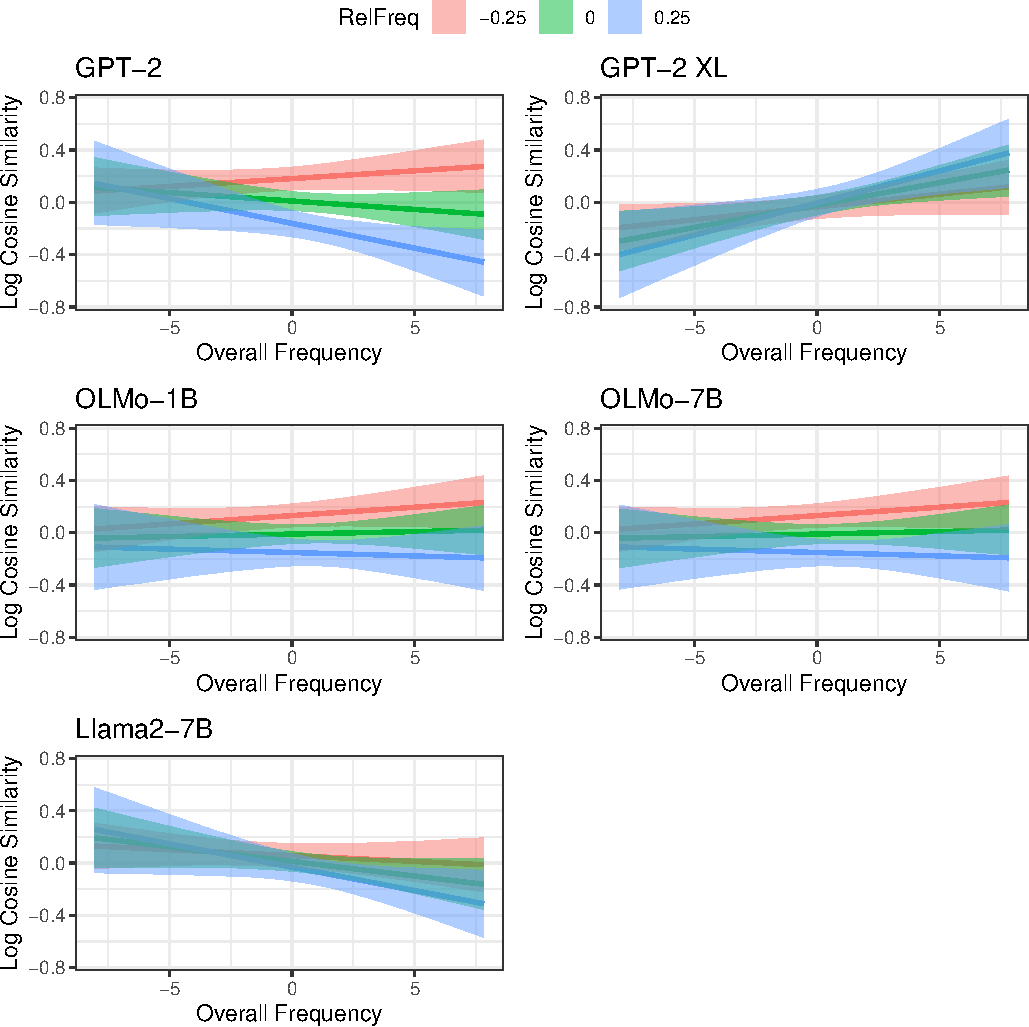
\includegraphics[keepaspectratio]{Chapters/LLM Storage/Writeup/writeup-llm-storage_files/figure-pdf/fig-modelsall-1.pdf}}

}

\end{figure}%

Overall we find a negative effect of relative frequency for GPT-2,
OLMo-1B, OLMo-7B, and Llama-2 7B. These results suggest that in general
for those models, the embeddings for the more frequent ordering of the
binomial (i.e., higher relative frequency) are less similar to the
compositional embeddings than the embeddings for the ordering of the
binomial that is less frequent are. Additionally, for these models there
is a negative interaction effect. This suggests that for high-frequency
binomials there is a stronger effect of relative frequency than for
low-frequency binomials. Specifically, the difference between the
embeddings for the frequent ordering of the binomials and the
compositional embeddings is even greater in high-frequency binomials
than low-frequency ones.

We also find mixed results for overall frequency, with GPT-2 XL showing
a strong effect of overall frequency such that the embeddings for
high-frequency binomials (ignoring relative frequency) are more similar
to the compositional embeddings than the embeddings for low-frequency
binomials are.

Finally, the interaction effect between relative frequency and overall
frequency is also in the opposite direction for GPT-2 XL compared to the
others. Specifically, for GPT-2 XL, as overall frequency increases, the
embeddings for the more frequent ordering of the binomials are
\emph{more} similar to the compositional embeddings than the embeddings
for the less frequent ordering are.

\subsection{Discussion}\label{discussion-8}

Our results suggest that for GPT-2, OLMo-1B, OLMo-7B, and Llama2-7B, the
representations of the more frequent form of the binomial diverges more
from the representation of the compositional form as a function of
overall frequency. That is, for low-frequency binomials, there is not
much of a difference between the embeddings of the more frequent form
and the compositional embeddings, however as the frequency of the
binomial increases, the embeddings of the more frequent form diverge
from the compositional embeddings.

Interestingly, this is not the case for GPT-2 XL, where the opposite
pattern is observed: as overall frequency increases, the representations
of the more frequent ordering of the binomial become even more similar
to the compositional representations. This suggests that not all large
language models are learning the same preferences and further that these
preferences may not be completely necessary to generate human-like text.

In summary, our results suggest that for high-frequency binomials in
most large language models, the semantic representation for the frequent
ordering of the binomial diverges more from the compositional
representation. This suggests that some large language models tend to
learn different representations for high-frequency binomials, similar to
what has been argued that humans do
(\citeproc{ref-morganAbstractKnowledgeDirect2016}{Morgan \& Levy,
2016a}). However, it's unclear on what timescale this emerges and at
what layers in the models this result holds for. For example, does this
difference emerge early in training or does it take a large amount of
training for these different representations to emerge? Further, since
different layers have been proposed to correspond to different functions
(e.g., earlier layers may represent more phonological knowledge while
later layers may represent more semantic knowledge;
\citeproc{ref-tenney2019bertrediscoversclassical}{Tenney et al., n.d.}),
it is possible that these results may be vary across different layers.
In Experiment 2 we examine both of these questions.

\section{Experiment 2}\label{experiment-2-2}

Experiment 2 is an exploratory analysis examining how representations
for binomials emerge throughout training across different hidden layers.
Specifically, since OLMo
(\citeproc{ref-groeneveldOLMoAcceleratingScience2024}{Groeneveld et al.,
2024}) released the model's checkpoints at various stages in the
training we can examine how our results in Experiment 1 emerge
throughout training. Further, since the model is open access we can also
examine the different hidden-layers of the model.

\subsection{Methods}\label{methods-9}

The methods in Experiment 2 were almost identical to those used in
Experiment 1, with two exceptions: first, rather than examining several
different large language models, we instead examined a single large
language model: OLMo 1B. OLMo 1B has released checkpoints at different
stages in learning. As such, we can examine the representations of
binomials at different stages of learning. Second, we also examined the
representations at each hidden layer in the model in order to examine
how the representation changes across layers.

For the present study, we examine the embeddings for the sentences in
Experiment 1 at each hidden layer at multiple different steps in the
training. In addition to examining the model after being trained, we
also examine the embeddings after being trained for 20000 (84B tokens),
40000 (168B tokens), 60000 (252B tokens), 80000 (336B tokens), and
100000 (419B tokens) steps.

\subsection{Results}\label{results-9}

A visualization of the embeddings at different layers and different
checkpoints is included in Figure~\ref{fig-resultsalllayers}.

\begin{landscape}

\begin{figure}[htbp]

\caption{\label{fig-resultsalllayers}A visualization of the cosine
similarity between the holistic embeddings and the compositional
embeddings for each hidden layer of each model checkpoint.}

\centering{

\pandocbounded{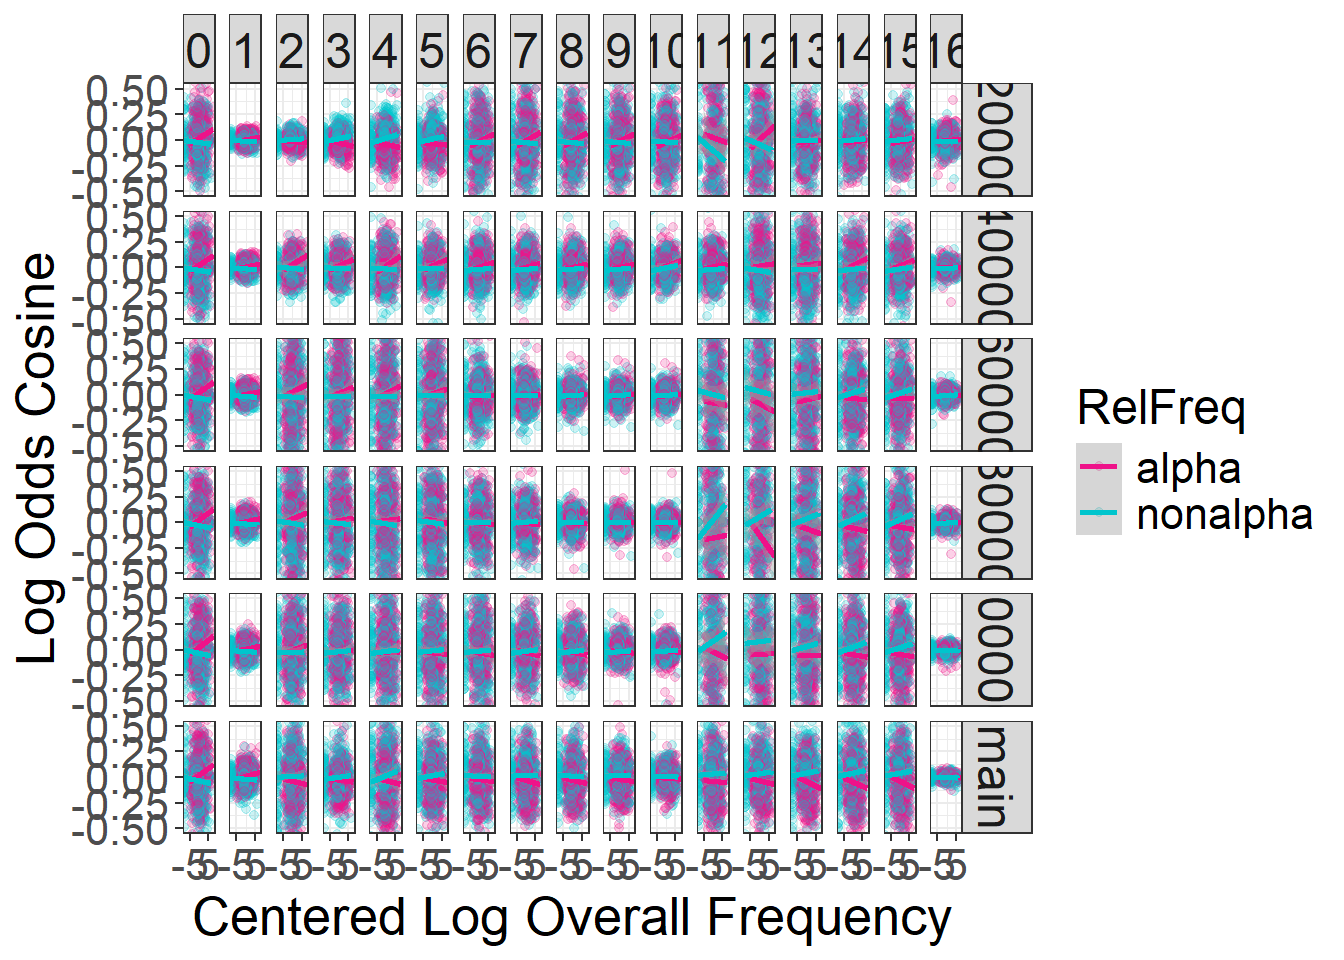
\includegraphics[keepaspectratio]{Chapters/LLM Storage/Writeup/writeup-llm-storage_files/figure-pdf/fig-resultsalllayers-1.pdf}}

}

\end{figure}%

\end{landscape}

There are two notable trends. First, the earlier layers tend to display
the opposite pattern from later layers, with the embeddings of the more
frequent ordering being more similar to the compositional embeddings.
Second, the holistic representation of the frequent ordering diverges
from the compositional representation at about the 80000th step (336B
tokens). We will discuss the implications of both of these in the
discussion section.

\subsection{Discussion}\label{discussion-9}

Our results demonstrate that the embeddings in the early layers are
relatively stable, with the model rapidly learning a holistic
representation of the more frequent ordering that is more similar to the
compositional representation than the less-frequent ordering is. On the
other hand, the differences in the later layers seem to emerge over
time.

These results are consistent with the general idea that later layers
encode more semantic information, since the pattern of the more frequent
embeddings diverging is seen in the later layers, while the earlier
layers show the opposite pattern. Indeed, since the binomials in both
orderings are similar phonologically (they contain the same sounds, just
in a different ordering), it may not be surprising that the divergence
occurs in later layers.

Additionally, while it may seem interesting that the embeddings seem to
converge in the last layer, it is not that surprising. The last layer in
transformer models tends to become specialized for the task (in this
case, next-word prediction). This specialization can become so extreme
as to become difficult to interpret representations at that level. For
example, Ethayarajh
(\citeproc{ref-ethayarajh2019howcontextualare}{n.d.}) found that any two
random words will on average have almost perfect cosine similarity in
the final layer of GPT-2. Thus, it is likely that the last layer of OLMo
may be similarly specialized, and the lack of a difference in cosine
similarity may be an artifact of task-specificity of the final layer.

Finally, the fact that the pattern emerges rather slowly (taking several
hundred billion tokens of training) suggests that the model must
experience the binomial a great number of times in order to learn a
separate representation for each ordering. This suggests that the model
isn't simply learning a separate representation because the binomial
occurs in different semantic contexts (because if that were the case we
would see the pattern emerge earlier on), but because it occurs
frequently. This is in line with usage-based theories that have argued
that holistic representations in humans emerge as a function of usage
(e.g., \citeproc{ref-bybee2003}{Bybee, 2003}).

\section{Conclusion}\label{conclusion-2}

The present study demonstrates that the semantic embeddings for the more
frequent ordering of a given binomial become less similar to the
compositional embeddings as a function of the overall frequency of the
binomial. That is, the embeddings of the more frequent ordering of a
high-frequency binomial (e.g., \emph{bread and butter}) are less similar
to the compositional embeddings than the embeddings of the less frequent
ordering (e.g., \emph{butter and bread}) are. Another way to frame these
results is that the same form (i.e., the same words) can give rise to
quantitatively (but systematically) different representations in large
language models as a function of the overall frequency of the binomial.

It may not seem particularly surprising that the more frequent form
diverges in semantic representation from the compositional form. After
all, by definition a large language model has more experience with the
more frequent form, which means the embeddings are being updated more
often for the more frequent ordering. This in turn creates more
opportunities for those embeddings to diverge from the compositional
embeddings. However, what is interesting is how this effect emerges over
time: early on in the training, the embeddings for the more frequent
form are more similar to the compositional form across both earlier and
later layers. Further, as training continues this stays the case for
early layers, but undergoes a reversal in later layers.

One possible explanation for our results is that the more frequent form
may be occurring in particularly different contexts from the
compositional and less frequent forms (e.g., perhaps they are more
idiomatic, such as \emph{black and white}\footnote{Although all of our
  sentences were sentences that encouraged a compositional reading of
  our binomials, and very few of our binomials had a particularly
  idiomatic meaning to begin with.}). However, if this was the case then
we would expect to see the embeddings for the frequent form to diverge
from the embeddings of the compositional form quite early in training.
Instead, however, we actually see the opposite early in the training:
the embeddings for the more frequent form are \emph{more} similar to
those of the compositional form and it takes time for these embeddings
to diverge.

Another possibility is that early on in training for high-frequency
binomials, the large language model's experience with the individual
words may largely overlap with the large language model's experience
with the frequent form of the binomial (e.g., the model's experience
with the binomial \emph{bread and butter} are also contributing to the
large language model's experience with each of the individual words).
Thus, initially these embeddings may be similar until the large language
model experiences the binomial enough times to learn different
representations. Specifically, as the model experiences more sentence
contexts with the binomial, the representation for the more frequent
ordering has more opportunities to diverge from the representation of
the individual words than the representation of the infrequent ordering
does (because the model is, by definition, encountering the more
frequent ordering of the binomial more). This process explains why the
same form can give rise to different representations.

Finally, our results can also be considered predictions for how humans
may learn representations. Future work would do well to examine whether
it is also the case that the semantic representations for the more
frequent ordering of high-frequency binomials diverge more from the
compositional representations in humans. Our results also make
predictions about the timescale of learning: for young children, the
pattern of results may actually be the opposite from adults, since at
earlier checkpoints in our model the embeddings for the more frequent
ordering of high-frequency binomials were more similar to the
compositional embeddings.

\bookmarksetup{startatroot}

\chapter{Frequency-dependent preference extremity arises from a
noisy-channel processing
model}\label{frequency-dependent-preference-extremity-arises-from-a-noisy-channel-processing-model}

\section{Introduction}\label{introduction-5}

Speakers are often confronted with many different ways to express the
same meaning. A customer might ask whether a store sells \emph{radios
and televisions} but they could have just as naturally asked whether the
store sells \emph{televisions and radios}. However, despite conveying
the same meaning, speakers sometimes have strong preferences for one
choice over competing choices (e.g., a preference for
\emph{men and women} over \emph{women and men};
\citeproc{ref-benorChickenEggProbabilistic2006}{Benor \& Levy, 2006};
\citeproc{ref-morganAbstractKnowledgeDirect2016}{Morgan \& Levy,
2016a}). These preferences are driven to some extent by generative
preferences (e.g., preference for short words before long words),
however they are sometimes violated by idiosyncratic preferences (e.g.,
\emph{ladies and
gentlemen} preferred despite a general men-before-women generative
preference; \citeproc{ref-morganAbstractKnowledgeDirect2016}{Morgan \&
Levy, 2016a}).

Interestingly, ordering preferences for certain constructions, such as
binomial expressions, are often more extreme for higher frequency items
(e.g., \emph{bread and butter}). That is, higher-frequency items
typically have more polarized preferences
(\citeproc{ref-liuFrequencydependentRegularizationConstituent2020}{Liu
\& Morgan, 2020},
\citeproc{ref-liuFrequencyDependentRegularizationSyntactic2021}{2021};
\citeproc{ref-morgan2015}{Morgan \& Levy, 2015},
\citeproc{ref-morganAbstractKnowledgeDirect2016}{2016a},
\citeproc{ref-morganFrequencydependentRegularizationIterated2016a}{2016b}).
This phenomenon is called
\emph{frequency-dependent preference extremity}, and while there is
evidence of it in several different constructions, it is still unclear
what processes this phenomenon is driven by. For example, it could be a
consequence of learning processes or a consequence of sentence
processing more broadly. In the present paper we examine whether a
noisy-channel processing model
(\citeproc{ref-gibsonRationalIntegrationNoisy2013}{Gibson, Bergen, et
al., 2013}) combined with transmission across generations
(\citeproc{ref-kirbyCumulativeCulturalEvolution2008}{Kirby et al.,
2008}; \citeproc{ref-realiEvolutionFrequencyDistributions2009}{Reali \&
Griffiths, 2009}) can account for frequency-dependent preference
extremity.

\subsection{Frequency-Dependent Preference
Extremity}\label{frequency-dependent-preference-extremity}

Frequency-dependent preference extremity has been documented for a
variety of different constructions in English
(\citeproc{ref-liuFrequencydependentRegularizationConstituent2020}{Liu
\& Morgan, 2020},
\citeproc{ref-liuFrequencyDependentRegularizationSyntactic2021}{2021};
\citeproc{ref-morgan2015}{Morgan \& Levy, 2015},
\citeproc{ref-morganFrequencydependentRegularizationIterated2016a}{2016b}).
For example, Morgan \& Levy (\citeproc{ref-morgan2015}{2015})
demonstrated that more frequent binomial expressions (e.g.,
\emph{bread and butter}) are more polarized (i.e., are preferred in one
order overwhelmingly more than the alternative). These ordering
preferences are also not simply a result of generative ordering
preferences (e.g., short words before long words;
\citeproc{ref-morganAbstractKnowledgeDirect2016}{Morgan \& Levy,
2016a}). Interestingly, Morgan \& Levy
(\citeproc{ref-morganFrequencydependentRegularizationIterated2016a}{2016b})
even showed that the distribution of binomial orderings at the
corpus-wide level are different than what would be expected given the
generative preferences for the binomials (see
Figure~\ref{fig-corpusplot1}).

\begin{figure}[htbp]

\caption{\label{fig-corpusplot1}The left plot is a plot of the relative
orderings of binomials in the corpus data from Morgan \& Levy
(\citeproc{ref-morgan2015}{2015}), the right is the plot of the
generative preferences of binomials in the same corpus. The x-axis is
proportion of occurrences in alphabetical order and the y-axis is the
probability density. The plot is reproduced from Morgan \& Levy
(\citeproc{ref-morganFrequencydependentRegularizationIterated2016a}{2016b}).}

\centering{

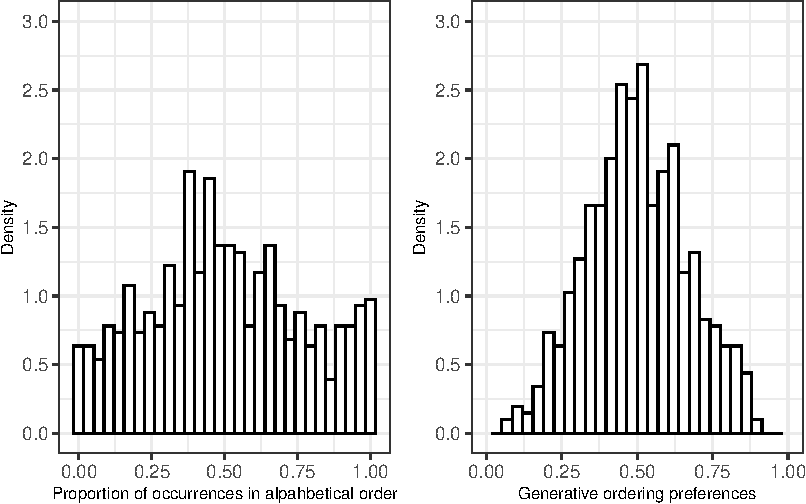
\includegraphics[width=0.8\linewidth,height=\textheight,keepaspectratio]{Chapters/frequency-dependent preference extremity/frequency-dependent-preference-extremity_files/figure-pdf/unnamed-chunk-2-1.pdf}

}

\end{figure}%

Additionally, Liu \& Morgan
(\citeproc{ref-liuFrequencydependentRegularizationConstituent2020}{2020})
demonstrated that the dative alternation in English also shows evidence
of frequency-dependent preference extremity (e.g., \emph{give}
\emph{the ball to him} vs \emph{give him the ball}). Specifically, they
demonstrated that higher frequency verbs have more polarized preferences
with respect to the dative alternation. Similarly, Liu \& Morgan
(\citeproc{ref-liuFrequencyDependentRegularizationSyntactic2021}{2021})
showed that in adjective-adjective-noun constructions, the adjective
orderings also show frequency-dependent preference extremity. That is,
adjectives in adjective-adjective-noun constructions with higher overall
frequencies (i.e., the summed counts of both orderings) show stronger
ordering preferences, even after taking into account generative
preferences of adjective orderings.

Interestingly, frequency-dependent preference extremity patterns
differently from rule-following regularization processes (e.g.,
morphological regularization) where it is the low-frequency items that
become more regular (rather than the high-frequency items;
\citeproc{ref-singletonWhenLearnersSurpass2004}{Singleton \& Newport,
2004}). For example, Schneider et al.
(\citeproc{ref-schneiderNoisyChannelModel2020}{2020}) demonstrated
through a noisy-channel processing model that regularization can arise
from learners attributing variation in the low-frequency items to noise.
On the other hand, frequency-dependent preference extremity patterns
more similarly to other processes, such as semantic entrenchment, where
it is the high-frequency items that develop strict preferences
(\citeproc{ref-harmonPuttingOldTools2017}{Harmon \& Kapatsinski, 2017};
\citeproc{ref-theakstonRoleEntrenchmentChildren2004}{Theakston, 2004}).
For example, people are generally more willing to accept a low-frequency
intransitive verb in a transitive context than a high-frequency
intransitive verb (e.g., \emph{He vanished it} is judged to be more
acceptable than \emph{He disappeared it};
\citeproc{ref-kapatsinski2018}{Kapatsinski, 2018};
\citeproc{ref-robenaltJudgmentEvidenceStatistical2015}{Robenalt \&
Goldberg, 2015};
\citeproc{ref-theakstonRoleEntrenchmentChildren2004}{Theakston, 2004}).

Why is it that it is the high-frequency items that develop more
polarized preferences in frequency-dependent preference extremity? One
possibility is that it occurs as an interaction between imperfect
learning and transmission across generations. For example, it's possible
that while learners of a language are in general very good at learning
the statistical patterns in the language (e.g.,
\citeproc{ref-saffranStatisticalLearning8MonthOld1996}{Saffran et al.,
1996}; \citeproc{ref-yuRapidWordLearning2007}{Yu \& Smith, 2007}), they
may do so imperfectly and with a bias towards preference extremity. If a
learner hears 70 tokens of \emph{bread and butter} and 30 tokens of
\emph{butter and bread}, they may imperfectly infer the ordering
preference and transmit the language with a more skewed distribution
(e.g., 75 tokens \emph{bread and butter} and 25 tokens of
\emph{butter and bread}). Indeed, previous studies have shown that
learners will reproduce the more frequent item at an even higher rate
than they heard it (\citeproc{ref-harmonPuttingOldTools2017}{Harmon \&
Kapatsinski, 2017}; \citeproc{ref-hudsonkamGettingItRight2009}{Hudson
Kam \& Newport, 2009}). As the language is transmitted from generation
to generation, it is possible this compounds until the highest-frequency
items develop polarized ordering preferences.

Following this logic, Morgan \& Levy
(\citeproc{ref-morganFrequencydependentRegularizationIterated2016a}{2016b})
investigated whether frequency-dependent preference extremity can arise
as a result of imperfect learning across generations. They found that a
data generation model with a frequency-\emph{independent} bias can
result in frequency-\emph{dependent} preference extremity across
generations of learners in a 2-alternative iterated learning paradigm.
They argued that frequency-dependent preference extremity emerges
because for low-frequency items, the preference extremity bias cannot
overcome the learner's generative preferences for maintaining variation,
but for high-frequency items, it can. In other words, for lower
frequency items, learners may rely more on their generative preferences
because they haven't heard the item very much. As the language is
transmitted across many generations, it may result in
frequency-dependent preference extremity.

While there is good evidence that a frequency-\emph{independent}
preference extremity bias can account for frequency-dependent preference
extremity across generations, it remains unclear what processes in
language transmission are analogous to this preference extremity bias.

\subsection{Noisy-Channel Processing}\label{noisy-channel-processing}

One possibility is that the frequency-independent preference extremity
bias is a product of noisy-channel processing
(\citeproc{ref-gibsonRationalIntegrationNoisy2013}{Gibson, Bergen, et
al., 2013}). Listeners are confronted with a great deal of noise in the
form of perception errors (e.g., a noisy environment) and even
production errors (speakers don't always say what they intended to;
\citeproc{ref-gibsonRationalIntegrationNoisy2013}{Gibson, Bergen, et
al., 2013}). In order to overcome these errors, a processing system must
take into account the noise of the system, for example by
probabilistically determining whether the perceived utterance was infact
intended by the speaker.

Indeed, there is evidence that our processing system does take noise
into account. For example, Ganong
(\citeproc{ref-ganongPhoneticCategorizationAuditory1980}{1980}) found
that people will process a non-word as being a word under noisy
conditions. Additionally, Felty et al.
(\citeproc{ref-feltyMisperceptionsSpokenWords}{n.d.}) demonstrated that
when listeners do misperceive a word, the word that they believe to have
heard tends to be higher frequency than the target word. Further, Keshev
\& Meltzer-Asscher (\citeproc{ref-keshevNoisyBetterRare2021}{2021})
found that in Arabic, readers will even process ambiguous subject/object
relative clauses as the more frequent interpretation, even if this
interpretation compromises subject-verb agreement. These results taken
together suggest that misperceptions may sometimes actually be a
consequence of noisy-channel processing (although it's worth noting that
good-enough processing theories also make very similar predictions,
e.g., \citeproc{ref-ferreiraGoodEnoughApproach2007}{Ferreira \& Patson,
2007}).

Further, people will even process \emph{grammatical} utterances, as a
more frequent or plausible interpretation
(\citeproc{ref-christiansonThematicRolesAssigned2001}{Christianson et
al., 2001}; \citeproc{ref-levyNoisychannelModelHuman2008}{Levy, 2008};
\citeproc{ref-poppelsStructuresensitiveNoiseInference2016}{Poppels \&
Levy, 2016}). This can even arise in two interpretations that cannot
both be consistent with the original sentence. For example, Christianson
et al. (\citeproc{ref-christiansonThematicRolesAssigned2001}{2001})
demonstrated that when people read the sentence
\emph{While the man hunted the deer ran into the woods}, people will
answer in the affirmative for both \emph{Did the man hunt the deer?} and
\emph{Did the dear run into the woods?}. Levy
(\citeproc{ref-levyNoisychannelModelHuman2008}{2008}) argued that this
phenonenon was explained by noisy-channel processing, since a single
insertion results in plausible, grammatical constructions for both
meanings (\emph{While the man hunted it the deer ran into the woods} vs
\emph{While the man hunted the deer it ran into the woods}).

In order to account for findings like these, Gibson, Piantadosi, et al.
(\citeproc{ref-gibsonNoisyChannelAccountCrosslinguistic2013}{2013})
developed a computational model that demonstrated how a system might
take into account noise (see
\citeproc{ref-levyNoisychannelModelHuman2008}{Levy, 2008} for a similar
approach). Specifically, their model operationalizes noisy-channel
processing as a Bayesian process where a listener estimates the
probability of the speaker's intended utterance given what they
perceived. Specifically, this is operationlized as being proportional to
the prior probability of the intended utterance multiplied by the
probability of the intended utterance being corrupted to the perceived
utterance (See Equation~\ref{eq-gibsonnoisy}):

\begin{equation}\phantomsection\label{eq-gibsonnoisy}{
P(S_i|S_p) \propto P(S_i) P(S_i \to S_p)
}\end{equation}

\noindent where \(P(S_i|S_p)\) is the probability of the intended
utterance given the perceived utterance, \(P(S_i)\) is the prior
probability of the intended utterance, and \(P(S_i \to S_p)\) is the
probability of the perceived utterance (\(S_p\)) given the intended
utterance (\(S_i\)). If the perceived utterance is
\emph{butter and bread}, for example, the listener can infer the
probability that the intended utterance was \emph{bread and butter} or
\emph{butter and bread}.

Gibson, Piantadosi, et al.
(\citeproc{ref-gibsonNoisyChannelAccountCrosslinguistic2013}{2013})'s
model made a variety of interesting predictions. For example, the model
predicted that when people are presented with an implausible sentence
(e.g., \emph{the mother gave the candle the daughter}), they should be
more likely to interpret the plausible version of the sentence (e.g.,
\emph{the mother gave the candle to the
daughter}) if there is increased noise (e.g., by adding syntactic errors
to the filler items, such as a deleted function word). Their model also
predicted that increasing the likelihood of implausible events (e.g., by
adding more filler items that were implausible, such as
\emph{the girl was kicked by the ball}) should increase the rate of
implausible interpretations of the sentence. Interestingly both of these
results were born out in their experimental data. In a follow up study,
Poppels \& Levy
(\citeproc{ref-poppelsStructuresensitiveNoiseInference2016}{2016})
further demonstrated that word-exchanges (e.g., \emph{The
ball kicked the girl} vs \emph{The girl kicked the ball}) are also taken
into account by comprehenders. These results taken together suggest that
humans do utilize a noisy-channel system in processing.

In addition to Gibson, Piantadosi, et al.
(\citeproc{ref-gibsonNoisyChannelAccountCrosslinguistic2013}{2013}),
previous research has demonstrated that noisy-channel processing models
may also account for certain types of regularization (e.g.,
\citeproc{ref-ferdinandCognitiveRootsRegularization2019}{Ferdinand et
al., 2019}; \citeproc{ref-schneiderNoisyChannelModel2020}{Schneider et
al., 2020}). For example, as mentioned earlier, Schneider et al.
(\citeproc{ref-schneiderNoisyChannelModel2020}{2020}) demonstrated that
a noisy-channel model can account for some rule-following regularization
processes (e.g., morphological regularization). However, it is unclear
whether noisy-channel processing models can also account for
frequency-dependent preference extremity.

\subsection{Present Study}\label{present-study-3}

Given the evidence of noisy-channel processing, it is possible that the
frequency-dependent preference extremity that Morgan \& Levy
(\citeproc{ref-morganFrequencydependentRegularizationIterated2016a}{2016b})
saw is a product of listeners' noisy-channel processing. Perhaps when
learners hear the phrase \emph{butter and bread}, they think the speaker
intended \emph{bread and butter}, which results in an activation of
\emph{bread and butter} even though they didn't hear it. This activation
could potentially even be stronger for \emph{bread and butter} than
\emph{butter and bread} in cases where the listener thinks the speaker
made a mistake. Further, this may compound over time for high-frequency
items, but not for low-frequency items. Thus, the present study examines
whether Gibson, Piantadosi, et al.
(\citeproc{ref-gibsonNoisyChannelAccountCrosslinguistic2013}{2013})'s
noisy-channel processing model can also predict frequency-dependent
preference extremity across generations of language transmission.

\section{Dataset}\label{dataset-2}

Following Morgan \& Levy
(\citeproc{ref-morganAbstractKnowledgeDirect2016}{2016a}), we use Morgan
\& Levy (\citeproc{ref-morgan2015}{2015})'s corpus of 594 Noun-Noun
binomial expressions (e.g., \emph{bread and butter}). There is evidence
that human binomial ordering preferences are driven by a combination of
generative preferences and observed preferences. Generative preferences
are abstract constraints on ordering preferences, such as a preference
for short words before long words, or male-coded terms before
female-coded terms. The observed preference for a given binomial is the
percentage that a given binomial occurs in alphabetical vs
nonalphabetical form. That is, if \emph{cats and dogs} appears 40 times
in a corpus, and \emph{dogs and cats} appears 60 times, then the
observed preference for the alphabetical form is 0.4. The corpus also
contains the overall frequency (total count of alphabetical and
nonalphabetical forms for a given binomial) which has been shown to
affect the strength of ordering preferences
(\citeproc{ref-morganAbstractKnowledgeDirect2016}{Morgan \& Levy,
2016a}). A detailed description of the constraints is listed below:

\begin{enumerate}
\def\labelenumi{\arabic{enumi}.}
\item
  The estimated generative preferences for each binomial, which are
  values between 0 and 1 representing the alphabetical ordering
  preferences (a neutral reference order), estimated from various
  phonological and semantic features that are known to influence
  binomial ordering preferences (\citeproc{ref-morgan2015}{Morgan \&
  Levy, 2015}). The generative constraints are calculated using Morgan
  \& Levy (\citeproc{ref-morgan2015}{2015})'s model. Values closer to
  zero represent a generative preference for the nonalphabetical order,
  while values closer to 1 represent a generative preference for the
  alphabetical order.
\item
  The observed binomial orderings preferences (hereafter: observed
  preferences) which are the proportion of binomial orderings that are
  in alphabetical order for a given binomial. A visualization of the
  distribution of observed preferences and generative preferences is
  included below in Figure~\ref{fig-corpusplot1}.
\item
  The overall frequency of a binomial expression (the frequency of AandB
  plus the frequency of BandA). Frequencies were obtained from the
  Google Books \emph{n}-grams corpus
  (\citeproc{ref-linSyntacticAnnotationsGoogle2012}{Lin et al., 2012}),
  which is orders of magnitude larger than the language experience of an
  individual speaker, and thus provides reliable frequency estimates for
  these expressions.
\end{enumerate}

\section{Model}\label{model}

Following Morgan \& Levy
(\citeproc{ref-morganFrequencydependentRegularizationIterated2016a}{2016b}),
we use a 2-alternative iterated learning paradigm. In our iterated
learning paradigm, at each generation, learners hear N tokens of a given
binomial with some in alphabetical (AandB) and some in nonalphabetical
(BandA) order. The learner's goal is to learn the ordering preferences
for each binomial. After hearing all N tokens, the learner then produces
N tokens to the next generation. This process then repeats. Morgan \&
Levy
(\citeproc{ref-morganFrequencydependentRegularizationIterated2016a}{2016b})
used a beta-binomial model: A learner has some prior over binomial
ordering preferences, which can be expressed as pseudocounts favoring
each order (e.g.\textasciitilde3 pseudocounts for AandB and 7 for
BandA). Each time the learner hears a binomial, they update their
beliefs by adding 1 count to the perceived order, e.g., if they heard
AandB, adding 1 AandB count. We modify this by instead having the
learner update their beliefs in proportion to what they believe the
intended order was: e.g., if they believe the intended utterance was
AandB with 50\% probability and BandA with 50\% probability, they will
add 0.5 to each count. These updated beliefs then influence their
beliefs about future intended utterances
(Equation~\ref{eq-gibsonnoisy}).

Specifically, the prior probability over the binomial ordering
preferences, (\(P(S_i)\)), follows Equation~\ref{eq-psi} and
Equation~\ref{eq-ptheta}. \(\alpha_1\) and \(\alpha_2\) are pseudocounts
of the alphabetical and nonalphabetical forms respectively.

\begin{equation}\phantomsection\label{eq-psi}{
S_i \sim Bernoulli(p_{theta})
}\end{equation}

\begin{equation}\phantomsection\label{eq-ptheta}{
p_{theta} \sim Beta(\alpha_1, \alpha_2)
}\end{equation}

After hearing a token, learners compute \(P(S_i = AandB|S_p)\) according
to Equation~\ref{eq-gibsonnoisy}. \(P(S_i \to S_p)\) is determined by a
fixed noise parameter, which we will call \(p_{noise}\). \(p_{noise}\)
represents the learner's belief of how likely a binomial ordering is to
have been swapped (i.e., AandB being swapped to BandA or vice versa).

To initialize \(p_{theta}\), and thus \(P(S_i)\), before the learner
hears any data, we used the mean and concentration parametrization of
the beta distribution. The mean (\(\mu\)) represents the expectation of
the distribution (the mean value of draws from the distribution). The
concentration parameter (\(\nu\)) describes how dense the distribution
is. Before the learner hears any data, \(\mu\) is equal to the
generative preference for the binomial (taken from
\citeproc{ref-morganFrequencydependentRegularizationIterated2016a}{Morgan
\& Levy, 2016b}). \(\nu\) is a free parameter, set to 10 for all
simulations in this paper.\footnote{Changing \(\nu\) does not
  qualitatively change the pattern of the results for any simulations in
  the paper, as long as it's greater than 2.} \(\alpha_1\) and
\(\alpha_2\) can also be expressed in terms of \(\mu\) and \(\nu\):

\begin{equation}\phantomsection\label{eq-alpha1}{
\alpha_1 = \mu \cdot \nu
}\end{equation}

\begin{equation}\phantomsection\label{eq-alpha2}{
\alpha_2 = (1-\mu) \cdot \nu
}\end{equation}

For all future tokens, learners will use the updated \(P(S_i)\) from the
previous token, where \(P(S_i = AandB)\) is the expectation of
\(p_\theta\). Crucially, this value will be different for each token of
learning due to the update that occurs on the previous token.

\begin{equation}\phantomsection\label{eq-expectationptheta}{
P(S_i = AandB) = \mathbb{E}(p_\theta)
}\end{equation}

We then use \(P(S_i)\) and \(p_{noise}\) to compute \(P(S_i|S_p)\),
following Equation~\ref{eq-gibsonnoisy}. If the perceived binomial is
alphabetical (AandB), we compute the unnormalized probability of the
alphabetical and nonalphabetical orderings according to the below
equations. Note that the process is comparable if the perceived binomial
is nonalphabetical.

\begin{equation}\phantomsection\label{eq-praw}{
P_{raw}(S_i = AandB|S_p = AandB) = P(S_i = AandB) \cdot (1 -  p_{noise})
}\end{equation}

\begin{equation}\phantomsection\label{eq-praw2}{
P_{raw}(S_i = BandA|S_p = AandB) = (1 - P(S_i = AandB)) \cdot p_{noise}
}\end{equation}

After calculating the unnormalized (raw) probabilities, they are then
normalized:

\begin{equation}\phantomsection\label{eq-phatalpha}{
\hat{p}_{\alpha} = \frac{P_{raw}(S_i = AandB|S_p = AandB)}{P_{raw}(S_i = AandB | S_p = AandB) + P_{raw}(S_i = BandA|S_p = AandB)}
}\end{equation}

\begin{equation}\phantomsection\label{eq-phatnotalpha}{
\hat{p}_{\neg\alpha} = 1 - \hat{p}_\alpha
}\end{equation}

\noindent where \(\hat{p}\alpha\) is the probability that the intended
binomial order was the alphabetical order, and \(\hat{p}{\neg\alpha}\)
is the probability that the intended binomial order was the
nonalphabetical order.

We then update \(\alpha_1'\) and \(\alpha2'\)to be used as the
parameters of \(p\theta\), and thus \(P(S_i)\), when the learner hears
the next token. This update is done according to the following equation:

\begin{equation}\phantomsection\label{eq-alpha1prime}{
\alpha_1' = \alpha_1 + \hat{p}_\alpha
}\end{equation}

\begin{equation}\phantomsection\label{eq-alpha2prime}{
\alpha_2' = \alpha_2 + \hat{p}_{\neg\alpha}
}\end{equation}

Note that when the learner hears any binomial, they update their beliefs
about the probability of both the alphabetical \emph{and}
nonalphabetical forms of the binomial (in proportion to how likely they
believe each ordering was intended by the speaker).

When the learner is done hearing N tokens and updating their beliefs of
\(P(S_i)\) for a given binomial, they then produce N tokens for the next
generation of learners. These are generated binomially, where
\(\theta = \mathbb{E}(p_\theta)\) is the inferred probability of the
alphabetical form of a given binomial. For the first generation of
speakers (before any learning has occurred), \(\theta\) is initialized
at 0.5.

When producing each token, there is also a possibility that the speaker
makes an error and produces an unintended ordering of the binomial. The
speaker error is analogous to a speaker choosing to produce a binomial
ordering (AandB or BandA), and then accidentally flipping it. For
example, perhaps they intended to say \emph{butter and bread}, but
accidentally said \emph{bread and butter} (or vice versa). Note that the
``unintended ordering'' is whichever order the speaker did not choose to
produce on that trial, regardless of the overall preference for the
binomial. In order to model this, the speaker produces a token in the
unintended order with probability \(p_{SpeakerNoise}\). This is a fixed
parameter in the model and remains constant across binomials and
generations.

This process continues iteratively for \(ngen\) generations.

\section{Results}\label{results-10}

We present our results in two main sections.\footnote{Scripts regarding
  simulations and results can be found here:
  \url{https://github.com/znhoughton/dissertation_writeup/tree/master/Chapters/Frequency-dependent\%20preference\%20extremity}}
The first section demonstrates the effects of the speaker and listener
noise parameters (\(p_{noise}\) and \(p_{SpeakerNoise}\) respectively)
on simulations of individual binomials. The aim of this section is to
examine whether the model can account for frequency-dependent preference
extremity across individual binomials varying in frequency.

The second section compares our model's predicted binomial orderings
across a range of binomials to the real-world corpus-wide distribution.
In this section, rather than simulating individual binomials, we
simulate the distribution of binomial orderings across the entire
dataset of binomials from Morgan \& Levy
(\citeproc{ref-morgan2015}{2015}) with the intent of examining whether
our model can capture the corpus-wide distribution.

\subsection{Speaker vs Listener Noise}\label{speaker-vs-listener-noise}

First we demonstrate that frequency-dependent preference extremity does
not arise when there is no listener or speaker noise. Instead we see
convergence to the prior, which is expected following Griffiths \&
Kalish (\citeproc{ref-griffithsLanguageEvolutionIterated2007}{2007}).
They demonstrated that when learners sample from the posterior in an
iterated learning paradigm, the stationary distribution converges to the
prior. To confirm this, we simulated the evolution of a single binomial
across 500 generations with various N (50, 100, 500, 1000, and 10,000).
The generative preference was 0.6. 1000 chains were run. We then
examined the model's inferred ordering preference in the final
generation. A visualization of the results is presented in
Figure~\ref{fig-noNoisePlot}.

\begin{figure}[htbp]

\caption{\label{fig-noNoisePlot}A plot of the distribution of simulated
binomials at the 500th generation, varying in frequency. The top value
represents N, which is the overall frequency of a binomial regardless of
ordering (i.e., count(AandB) + count(BandA)). On the x-axis is the
predicted probability of producing the binomial in alphabetical form. On
the y-axis is probability density. Speaker and listener noise was set to
0. The generative preference was 0.6, and nu was set to 10. 1000 chains
were run. Note that all values of N produce dense distributions
clustered around 0.6 (i.e., there is no frequency-dependent preference
extremity).}

\centering{

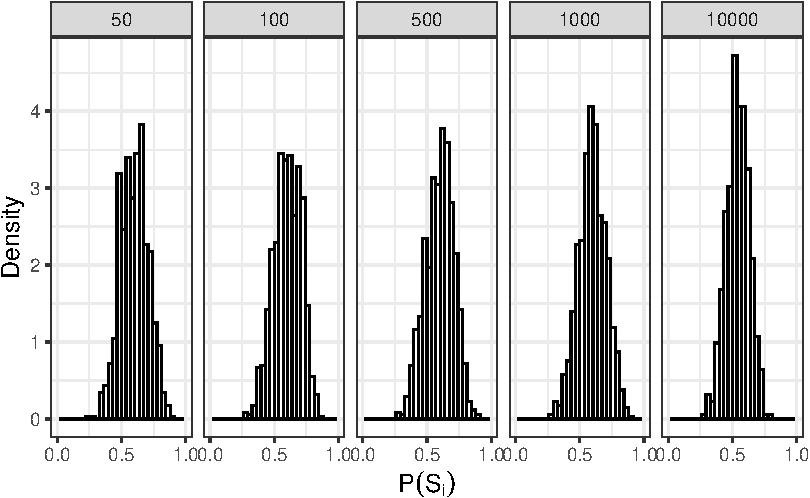
\includegraphics[width=1\linewidth,height=\textheight,keepaspectratio]{Chapters/frequency-dependent preference extremity/frequency-dependent-preference-extremity_files/figure-pdf/fig-noNoisePlot-1.pdf}

}

\end{figure}%

We then systematically manipulated N, listener noise (\(p_{noise}\)) and
speaker noise (\(p_{SpeakerNoise}\)). Specifically, we varied N across
100, 1000, and 10000, and listener and speaker noise were varied across
0, 0.033, 0.066, and 0.1. We ran simulations for every combination of
these values (Figure~\ref{fig-fullsimsplot}). For these simulations, the
generative preference was set to 0.6 and 1000 chains were run across 500
generations.

Our results suggest that frequency-dependent preference extremity does
arise from the model when noise is introduced, but only if listener
noise is greater than speaker noise. Further our results demonstrate
that if listener noise is greater than speaker noise, then the greater
the difference between the listener and speaker noise, the stronger the
preference extremity effect (this is demonstrated by moving vertically
down the column labeled \(p_{SpeakerNoise} = 0\) in
Figure~\ref{fig-fullsimsplot}).

Interestingly this preference extremity disappears if the listener's
noise parameter is less than or equal to the speaker's noise parameter.
For example, notice how if you split the plot along the diagonal, all
the plots on the top half, including the diagonal, show no evidence of
preference extremity. These graphs are all visualizations where the
speaker noise is greater than or equal to the listener noise.

\begin{landscape}

\begin{figure}[htbp]

\caption{\label{fig-fullsimsplot}Our simulation results for every
combination of speaker noise, listener noise, and N. Note that there is
an increase in ordering preference extrmity as N increases when listener
noise is greater than speaker noise. N corresponds to the overall
frequency of the binomial (count of AandB plus count of BandA) and
varies across 10, 100, and 1000. Both speaker and listener noise were
varied across 0, 0.033, 0.066, and 0.1. The distributions in the plot
demonstrate the inferred ordering preference at the 500th generation.}

\centering{

\pandocbounded{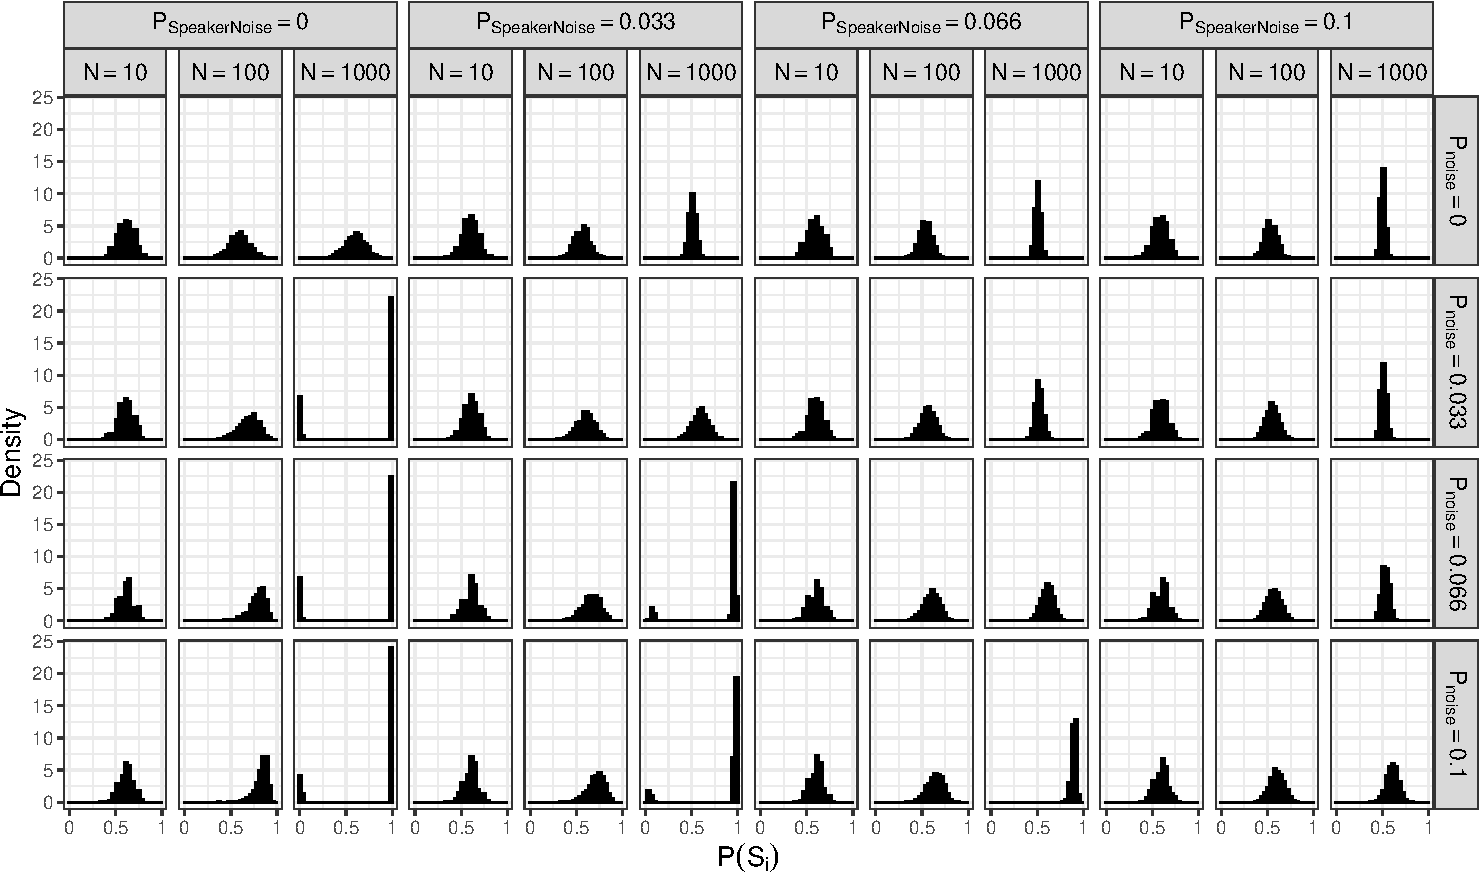
\includegraphics[keepaspectratio]{Chapters/frequency-dependent preference extremity/frequency-dependent-preference-extremity_files/figure-pdf/fig-fullsimsplot-1.pdf}}

}

\end{figure}%

\end{landscape}

It is useful to revisit here what the speaker and listener noise
parameters represent. The speaker noise parameter is how often the
speaker produces an error and the listener noise parameter is the
listeners' belief of how noisy the environment is. Note that a speaker
error here is not whether the speaker produces the more frequent
binomial ordering, but rather whether the speaker produces the intended
binomial ordering. In other words, if a speaker intends to produce
\emph{butter and bread}, and instead produces \emph{bread and butter},
this is an error in our model. Framed this way, one explanation for our
results is that when the listener is inferring more noise than the
speakers are producing, they are relying more on their inferences, which
can become more and more extreme. On the other hand, if they're not
inferring enough noise, then they are relying more on the data. The
greater the speaker noise, due to how we operationalized speaker noise,
the more balanced the data will be.

Thus our model makes a novel prediction: In order to account for
frequency-dependent preference extremity, listeners must be inferring
more noise than speakers are actually producing.

\subsection{Corpus Data}\label{corpus-data}

Finally, we now demonstrate that our model also predicts the
language-wide distribution of binomial preference strengths seen in the
corpus data. In order to demonstrate this, we simulated model
predictions for all 594 binomials from Morgan \& Levy (2015). The model
estimated the ordering preference across 500 generations with 10 chains
each. Values for the generative preference and N for each binomial were
taken from Morgan \& Levy (\citeproc{ref-morgan2015}{2015})'s corpus.
Listener noise was set to 0.02 and speaker noise to 0.005. Note that we
scale N based on an estimated lifetime exposure of 300 million tokens
(\citeproc{ref-levyProcessingExtraposedStructures2012}{Levy et al.,
2012}).

Our results demonstrate that our model can approximate the distribution
in the corpus data (See Figure~\ref{fig-corpusourmodel}). In other
words, the corpus-wide distribution of binomial orderings according to
our model is similar to the ordering we see in actual corpus data.
Further, the distribution is qualitatively similar regardless of
listener and speaker noise parameters, as long as listener noise is
greater than speaker noise. Altogether, this suggests that our model
both captures the phenomenon of frequency-dependent preference
extremity, but also in capturing it our model also predicts a similar
distribution of binomial orderings to what we see in corpus data.

\begin{figure}[htbp]

\caption{\label{fig-corpusourmodel}A plot of the stationary distribution
of ordering preferences in the corpus data from Morgan \& Levy
(\citeproc{ref-morgan2015}{2015}) and the distribution of ordering
preferences after 500 generations of our iterated learning model (left
and right respectively). For our simulations, the binomial frequencies
and generative preferences were matched with the corpus data. Listener
noise was set to 0.02, and speaker noise was set to 0.005.}

\centering{

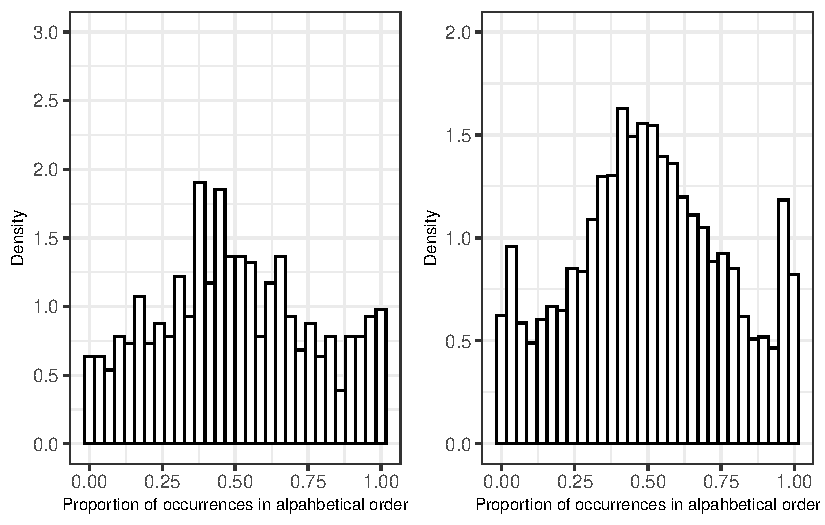
\includegraphics[width=0.8\linewidth,height=\textheight,keepaspectratio]{Chapters/frequency-dependent preference extremity/frequency-dependent-preference-extremity_files/figure-pdf/fig-corpusourmodel-1.pdf}

}

\end{figure}%

\section{Conclusion}\label{conclusion-3}

The present study examined whether a noisy-channel processing model
(\citeproc{ref-gibsonNoisyChannelAccountCrosslinguistic2013}{Gibson,
Piantadosi, et al., 2013}) integrated in an iterated learning model
(\citeproc{ref-morganFrequencydependentRegularizationIterated2016a}{Morgan
\& Levy, 2016b}) can capture the effects of frequency-dependent
preference extremity. Our results demonstrate that frequency-dependent
preference extremity can emerge from a noisy-channel processing model
when listeners infer more noise in the environment than the speakers
actually produce. Our results also make novel predictions. For example,
if our current model is accurate, it suggests that listeners assume more
noise than the speakers produce. Further, it suggests that for
high-frequency binomials, such as \emph{butter and bread}, hearing
\emph{butter and bread} may activate \emph{bread and butter} more
strongly than \emph{butter and bread}. Finally, it seems more unlikely
that a speaker would unintentionally produce the unintended ordering for
high-frequency binomials than low-frequency binomials (e.g., producing
\emph{butter and bread,} when they mean to say \emph{bread and butter)}.
Thus it will also be interesting to examine models that don't use a
fixed speaker-noise parameter.

\bookmarksetup{startatroot}

\chapter{Conclusion}\label{conclusion-4}

In this dissertation I have shown evidence that both frequency and
predictability lead to multi-word phrases being stored. Further, I have
demonstrated that stored items can lose part of their internal structure
as a function of usage. Additionally, I have demonstrated that large
language models trade off between stored and generative knowledge in
ways that are both similar and dissimilar to humans. Finally, I have
demonstrated that positing multi-word storage can account for certain
features of language change, specifically frequency-dependent preference
extremity.

I have also argued that theories of processing and learning must account
for multi-word storage. Many of the processing theories today still
assume, either explicitly or implicitly, that each sentence is broken
down into individual words that are then combined using knowledge of the
grammar. However, positing multi-word holistic storage will lead to a
new, rich set of predictions and questions.

At the beginning of this dissertation, I posited three questions: 1)
what factors determine whether a phrase is stored holistically or
generated compositionally? 2) What are the processing consequences for
holistic storage? And 3) How are holistically stored phrases
represented? In this section, I return to each of the questions and
explore what we've learned. I will then explore future questions and
what their answers may tell us.

\section{Revisiting our questions}\label{revisiting-our-questions}

In this dissertation I have presented evidence that both frequency and
predictability drive storage. I have shown, for example, that \emph{up}
is harder for participants to recognize in high-frequency or
high-predictability phrases than in medium-frequency or
medium-predictability phrases. I have also shown that models of learning
(large language models) predict that learners rely on item-specific
knowledge for binomials that they have experienced before. Further, they
also predict that the representations of high-frequency binomials
diverge more from their compositional representations than low-frequency
binomials.

Additionally, I demonstrated that holistically stored representations
cannot be accessed after hearing only the first word in the phrase. In
other words, it is possible that participants don't access the phrase
until they have enough acoustic information to disambiguate between the
phrase and its competitors. Further, I argue that the representation of
the phrase competes with the representations of the individual words,
causing a slowdown in recognition time for the individual words that
comprise the phrase. These results demonstrate the importance of
expanding current areas of the literature, such as the word-recognition
literature, to include the topic of multi-word holistic storage.

Finally, in this dissertation I have argued that storage arises
naturally as a function of our learning mechanisms. Multi-word storage
is a natural product of association frequent and/or predictable events
with each other. However, what are the implications of this for language
learning and processing more broadly. In the next section I discuss the
future of these questions and why the field should care.

\section{What is next?}\label{what-is-next}

Both frequency and predictability drive storage. However, what does this
mean? Are they two measurements of the same underlying cognitive
process? It is possible that frequency effects are a result of
automatization while predictability effects may be a consequence of
learning. For example, as people perform a sequence of motor actions
more often (i.e., as the sequence of motor actions becomes more
frequent), humans become able to perform the sequence more quickly and
more fluidly (\citeproc{ref-sosnik2004whenpracticeleads}{Sosnik et al.,
2004}). It is possible that frequency effects on storage are a result of
a similar process: as people use a phrase more often, it becomes more
automatic and this results in it being stored separately.

On the other hand, learners are not simply sensitive to how frequent a
cue occurs with an outcome, but also to how predictive a cue is of an
outcome (e.g.,
\citeproc{ref-ramscarChildrenValueInformativity2013}{Ramscar et al.,
2013}). Thus, it is possible that rather than automatization,
predictability drives storage because predictable things are simply
learned as a single chunk.

Future work will do well to examine whether this prediction is born out.
For example, if frequency effects are a result of automatization and
predictability effects are a result of learning, then frequency may lead
to storage of a phrase over time as it becomes used more often, while
predictability may lead to storage immediately due to learning the
phrase as a single unit.

Additionally, very few theories of processing expressly account for
multi-word storage
(\citeproc{ref-morganFormalizingConstructionGrammar}{Morgan et al.,
2023}; c.f., fragment grammar theories; e.g.,
\citeproc{ref-odonnellFragmentGrammarsExploring2009}{O'Donnell et al.,
2009}). This is important because most phrases that are stored
holistically can also be formed compositionally. For example, storing
the phrase \emph{I don't know} holistically does not preclude the
learner from generating the phrase compositionally. When do humans
access the holistic representation instead of generating it
compositionally from its component parts? This is not an easy question
to answer and may vary as a function of the task that people are engaged
in. It seems more likely that someone would access the phrase
holistically in production than perception, for example, because in
production the speaker has a meaning they wish to convey. However, in
perception it is less clear. For example, when listening to a sentence,
the listener must by definition listen in a temporally linear manner
(i.e., word-by-word). As such, does the listener wait until hearing the
phrase before accessing any of the parts? Despite the difficulty of this
question, it is important an important one for the processing literature
to address.

Finally, what role will transformer models play in future work on
language learning and processing? First, as I have argued in this
dissertation, (transformer) language models are the first models of
language that are able to produce fluent, human-like text. However,
there are other important reasons to take a closer look at these models
as well. First, they learn in a way that resembles, to some extent,
human-learning. Specifically, the learning mechanism in both humans and
language models is prediction-error. In other words, language models are
a model of language learning. However, it is also the case that there
are significant differences between humans and language models. For
example, language models require a lot more data than humans.\footnote{Although
  I have made the case throughout this dissertation that this is not a
  fair comparison, given that each encounter a human has with a word
  contains a great deal of contextual information that language models
  don't get, such as visual and audio cues.} This difference in the
amount of data that language models and humans experience has been a
source of a great deal of criticism. However, there have been recent
attempts to bridge this gap. For example, several recent studies have
taken the initiative of training smaller language models (e.g.,
\citeproc{ref-misraLanguageModelsLearn2024}{Misra \& Mahowald, 2024};
\citeproc{ref-yaoBothDirectIndirect2025}{Yao et al., 2025}) using an
amount of data comparable to humans. This method allows for more direct
comparisons between models and human behavioral studies because it
allows for complete control over the models training and testing
environments. By manipulating the training data of language models, it
is possible to more carefully examine what factors affect the tradeoff
between computation and storage.

\bookmarksetup{startatroot}

\chapter*{References}\label{references}
\addcontentsline{toc}{chapter}{References}

\markboth{References}{References}

\begingroup
\raggedright

\phantomsection\label{refs}
\begin{CSLReferences}{1}{0}
\bibitem[\citeproctext]{ref-al-selwiLSTMInefficiencyLongterm2023}
Al-Selwi, S. M., Hassan, M. F., Abdulkadir, S. J., \& Muneer, A. (2023).
LSTM inefficiency in long-term dependencies regression problems.
\emph{Journal of Advanced Research in Applied Sciences and Engineering
Technology}, \emph{30}(3), 1631.
\url{https://www.researchgate.net/profile/Amgad-Muneer-2/publication/370769893_LSTM_Inefficiency_in_Long-Term_Dependencies_Regression_Problems/links/64624134f43b8a29ba525b9b/LSTM-Inefficiency-in-Long-Term-Dependencies-Regression-Problems.pdf}

\bibitem[\citeproctext]{ref-ambridgeStoredAbstractionsRadical2020}
Ambridge, B. (2020). Against stored abstractions: A radical exemplar
model of language acquisition. \emph{First Language}, \emph{40}(5-6),
509--559. \url{https://doi.org/10.1177/0142723719869731}

\bibitem[\citeproctext]{ref-arnonMoreWordsFrequency2010}
Arnon, I., \& Snider, N. (2010). More than words: Frequency effects for
multi-word phrases. \emph{Journal of Memory and Language}, \emph{62}(1),
67--82. \url{https://doi.org/10.1016/j.jml.2009.09.005}

\bibitem[\citeproctext]{ref-baayenDutchInflectionRules2002}
Baayen, H., Schreuder, R., De Jong, N., \& Krott, A. (2002). \emph{Dutch
inflection: The rules that prove the exception} (S. Nooteboom, F.
Weerman, \& F. Wijnen, Eds.; Vol. 30, pp. 61--92). Springer Netherlands.
\url{http://link.springer.com/10.1007/978-94-010-0355-1_3}

\bibitem[\citeproctext]{ref-baayenAmorphousModelMorphological2011}
Baayen, R. H., Milin, P., rević, D. F., Hendrix, P., \& Marelli, M.
(2011). An amorphous model for morphological processing in visual
comprehension based on naive discriminative learning.
\emph{Psychological Review}, \emph{118}(3), 438--481.
\url{https://doi.org/10.1037/a0023851}

\bibitem[\citeproctext]{ref-bannardStoredWordSequences2008}
Bannard, C., \& Matthews, D. (2008). Stored Word Sequences in Language
Learning: The Effect of Familiarity on Children's Repetition of
Four-Word Combinations. \emph{Psychological Science}, \emph{19}(3),
241--248. \url{https://doi.org/10.1111/j.1467-9280.2008.02075.x}

\bibitem[\citeproctext]{ref-bansal2018functionfailuresensory}
Bansal, S., Ford, J. M., \& Spering, M. (2018). The function and failure
of sensory predictions. \emph{Annals of the New York Academy of
Sciences}, \emph{1426}(1), 199--220.
\url{https://doi.org/10.1111/nyas.13686}

\bibitem[\citeproctext]{ref-barrRandomEffectsStructure2013}
Barr, D. J., Levy, R., Scheepers, C., \& Tily, H. J. (2013). Random
effects structure for confirmatory hypothesis testing: Keep it maximal.
\emph{Journal of Memory and Language}, \emph{68}(3), 255--278.
\url{https://doi.org/10.1016/j.jml.2012.11.001}

\bibitem[\citeproctext]{ref-benderDangersStochasticParrots2021}
Bender, E. M., Gebru, T., McMillan-Major, A., \& Shmitchell, S. (2021).
\emph{FAccT '21: 2021 ACM Conference on Fairness, Accountability, and
Transparency}. 610--623. \url{https://doi.org/10.1145/3442188.3445922}

\bibitem[\citeproctext]{ref-bender2020climbingnlumeaning}
Bender, E. M., \& Koller, A. (2020). \emph{Climbing towards NLU: On
meaning, form, and understanding in the age of data}. 51855198.
\url{https://aclanthology.org/2020.acl-main.463/}

\bibitem[\citeproctext]{ref-bengioProblemLearningLongterm1993}
Bengio, Y., Frasconi, P., \& Simard, P. (1993). \emph{IEEE international
conference on neural networks}. 1183--1188 vol.3.
\url{https://doi.org/10.1109/ICNN.1993.298725}

\bibitem[\citeproctext]{ref-benorChickenEggProbabilistic2006}
Benor, S. B., \& Levy, R. (2006). The chicken or the egg? A
probabilistic analysis of english binomials. \emph{Language},
\emph{82}(2), 233--278. \url{https://doi.org/10.1353/lan.2006.0077}

\bibitem[\citeproctext]{ref-berkoChildsLearningEnglish1958}
Berko, J. (1958). The Child's Learning of English Morphology.
\emph{{\emph{WORD}}}, \emph{14}(2-3), 150--177.
\url{https://doi.org/10.1080/00437956.1958.11659661}

\bibitem[\citeproctext]{ref-boyceMazeMadeEasy2020}
Boyce, V., Futrell, R., \& Levy, R. P. (2020). Maze made easy: Better
and easier measurement of incremental processing difficulty.
\emph{Journal of Memory and Language}, \emph{111}(November 2019),
104082. \url{https://doi.org/10.1016/j.jml.2019.104082}

\bibitem[\citeproctext]{ref-burknerBrmsPackageBayesian2017}
Bürkner, P.-C. (2017). Brms: An r package for bayesian multilevel models
using stan. \emph{Journal of Statistical Software}, \emph{80}, 128.
\url{https://www.jstatsoft.org/article/view/v080i01}

\bibitem[\citeproctext]{ref-bybeeWordFrequencyContext2002}
Bybee, J. (2002). Word frequency and context of use in the lexical
diffusion of phonetically conditioned sound change. \emph{Language
Variation and Change}, \emph{14}(3), 261--290.
\url{https://doi.org/10.1017/S0954394502143018}

\bibitem[\citeproctext]{ref-bybee2003}
Bybee, J. (2003). \emph{Phonology and language use} (Vol. 94). Cambridge
University Press.

\bibitem[\citeproctext]{ref-bybee2001}
Bybee, J., \& Hopper, P. (2001). Introduction to frequency and the
emergence of linguistic structure. \emph{Typological Studies in
Language}, \emph{45}, 126.
\url{https://www.torrossa.com/gs/resourceProxy?an=5002168&publisher=FZ4850\#page=10}

\bibitem[\citeproctext]{ref-bybeeEffectUsageDegrees1999}
Bybee, J., \& Scheibman, J. (1999). The effect of usage on degrees of
constituency: The reduction of don't in english. \emph{Linguistics},
\emph{37}(4). \url{https://doi.org/10.1515/ling.37.4.575}

\bibitem[\citeproctext]{ref-chomsky1965}
Chomsky, N. (1965). \emph{Aspects of the theory of syntax special
technical report no. 11}.

\bibitem[\citeproctext]{ref-christiansenMoreWordsRole2017}
Christiansen, M. H., \& Arnon, I. (2017). More than words: The role of
multiword sequences in language learning and use. \emph{Topics in
Cognitive Science}, \emph{9}(3), 542--551.
\url{https://doi.org/10.1111/tops.12274}

\bibitem[\citeproctext]{ref-christiansonThematicRolesAssigned2001}
Christianson, K., Hollingworth, A., Halliwell, J. F., \& Ferreira, F.
(2001). Thematic roles assigned along the garden path linger.
\emph{Cognitive Psychology}, \emph{42}(4), 368--407.
\url{https://doi.org/10.1006/cogp.2001.0752}

\bibitem[\citeproctext]{ref-clark2013arewepredictive}
Clark, A. (2013). Are we predictive engines?: Perils, prospects, and the
puzzle of the porous perceiver. \emph{Behavioral and Brain Sciences},
\emph{36}(3), 233253.
\url{https://www.research.ed.ac.uk/en/publications/are-we-predictive-engines-perils-prospects-and-the-puzzle-of-the-}

\bibitem[\citeproctext]{ref-clark2019whatdoesbert}
Clark, K., Khandelwal, U., Levy, O., \& Manning, C. D. (2019).
\emph{BlackboxNLP 2019} (T. Linzen, G. Chrupała, Y. Belinkov, \& D.
Hupkes, Eds.; p. 276286). Association for Computational Linguistics.
\url{https://doi.org/10.18653/v1/W19-4828}

\bibitem[\citeproctext]{ref-coltheart1977access}
Coltheart, M., Davelaar, E., Jonasson, J. T., \& Besner, D. (1977).
Access to the internal lexicon. In \emph{Attention and performance VI}
(pp. 535--555). Routledge.

\bibitem[\citeproctext]{ref-cooper1975worldorder}
Cooper, W. E., \& Ross, J. R. (1975). World order. \emph{Papers from the
Parasession on Functionalism}, \emph{11}, 63111.

\bibitem[\citeproctext]{ref-ethayarajh2019howcontextualare}
Ethayarajh, K. (n.d.). \emph{How contextual are contextualized word
representations? Comparing the geometry of BERT, ELMo, and GPT-2
embeddings}. \url{https://doi.org/10.48550/arXiv.1909.00512}

\bibitem[\citeproctext]{ref-feltyMisperceptionsSpokenWords}
Felty, R. A., Buchwald, A., Gruenenfelder, T. M., \& Pisoni, D. B.
(n.d.). Misperceptions of spoken words: Data from a random sample of
american english words. \emph{The Journal of the Acoustical Society of
America}, \emph{134}, 572--585.
\url{https://www.robfelty.com/academic-files/docs/FeltyEtAl2013.pdf}

\bibitem[\citeproctext]{ref-ferdinandCognitiveRootsRegularization2019}
Ferdinand, V., Kirby, S., \& Smith, K. (2019). The cognitive roots of
regularization in language. \emph{Cognition}, \emph{184}, 53--68.
\url{https://doi.org/10.1016/j.cognition.2018.12.002}

\bibitem[\citeproctext]{ref-ferreira2018integrationpredictionlanguage}
Ferreira, F., \& Chantavarin, S. (2018). Integration and Prediction in
Language Processing: A Synthesis of Old and New. \emph{Current
Directions in Psychological Science}, \emph{27}(6), 443--448.
\url{https://doi.org/10.1177/0963721418794491}

\bibitem[\citeproctext]{ref-ferreiraGoodEnoughApproach2007}
Ferreira, F., \& Patson, N. D. (2007). The {`}Good Enough{'} Approach to
Language Comprehension. \emph{Language and Linguistics Compass},
\emph{1}(1-2), 71--83.
\url{https://doi.org/10.1111/j.1749-818X.2007.00007.x}

\bibitem[\citeproctext]{ref-ganongPhoneticCategorizationAuditory1980}
Ganong, W. F. (1980). Phonetic categorization in auditory word
perception. \emph{Journal of Experimental Psychology: Human Perception
and Performance}, \emph{6}(1), 110.
\url{https://psycnet.apa.org/record/1981-07020-001}

\bibitem[\citeproctext]{ref-gibsonRationalIntegrationNoisy2013}
Gibson, E., Bergen, L., \& Piantadosi, S. T. (2013). Rational
integration of noisy evidence and prior semantic expectations in
sentence interpretation. \emph{Proceedings of the National Academy of
Sciences}, \emph{110}(20), 8051--8056.
\url{https://doi.org/10.1073/pnas.1216438110}

\bibitem[\citeproctext]{ref-gibsonNoisyChannelAccountCrosslinguistic2013}
Gibson, E., Piantadosi, S. T., Brink, K., Bergen, L., Lim, E., \& Saxe,
R. (2013). A noisy-channel account of crosslinguistic word-order
variation. \emph{Psychological Science}, \emph{24}(7), 1079--1088.
\url{https://doi.org/10.1177/0956797612463705}

\bibitem[\citeproctext]{ref-goel2013wholegreatersum}
Goel, V., Mishra, A., Alahari, K., \& Jawahar, C. V. (2013). \emph{Whole
is greater than sum of parts: Recognizing scene text words}. 398402.
\url{https://ieeexplore.ieee.org/abstract/document/6628652/?casa_token=PNkOeMtKlv4AAAAA:fSbWtdvLuDlSqk9otMLUV05tfECv2bdPu7rbC9RR1Lngjra3gkFMF9DPOPrvQHvPmffD2uh4}

\bibitem[\citeproctext]{ref-goldbergConstructionsNewTheoretical2003}
Goldberg, A. E. (2003). Constructions: A new theoretical approach to
language. \emph{Trends in Cognitive Sciences}, \emph{7}(5), 219--224.
\url{https://doi.org/10.1016/S1364-6613(03)00080-9}

\bibitem[\citeproctext]{ref-goldinger1989priminglexicalneighbors}
Goldinger, S. D., Luce, P. A., \& Pisoni, D. B. (1989). Priming lexical
neighbors of spoken words: Effects of competition and inhibition.
\emph{Journal of Memory and Language}, \emph{28}(5), 501518.
\url{https://www.sciencedirect.com/science/article/pii/0749596X89900090}

\bibitem[\citeproctext]{ref-griffithsLanguageEvolutionIterated2007}
Griffiths, T. L., \& Kalish, M. L. (2007). Language evolution by
iterated learning with bayesian agents. \emph{Cognitive Science},
\emph{31}(3), 441--480. \url{https://doi.org/10.1080/15326900701326576}

\bibitem[\citeproctext]{ref-groeneveldOLMoAcceleratingScience2024}
Groeneveld, D., Beltagy, I., Walsh, P., Bhagia, A., Kinney, R., Tafjord,
O., Jha, A. H., Ivison, H., Magnusson, I., Wang, Y., et al. (2024).
Olmo: Accelerating the science of language models. \emph{arXiv Preprint
arXiv:2402.00838}.

\bibitem[\citeproctext]{ref-gulordava2018colorlessgreenrecurrent}
Gulordava, K., Bojanowski, P., Grave, E., Linzen, T., \& Baroni, M.
(2018). Colorless green recurrent networks dream hierarchically.
\emph{arXiv Preprint arXiv:1803.11138}.

\bibitem[\citeproctext]{ref-haleyThisBERTNow2020}
Haley, C. (2020). \emph{This is a BERT. Now there are several of them.
Can they generalize to novel words?} 333341.
\url{https://aclanthology.org/2020.blackboxnlp-1.31/}

\bibitem[\citeproctext]{ref-hampeTransitivePhrasalVerbs2012}
Hampe, B. (2012). Transitive phrasal verbs in acquisition and use: A
view from construction grammar. \emph{Language Value}, \emph{4}(1),
1--32.
\url{https://raco.cat/index.php/LanguageValue/article/view/302086}

\bibitem[\citeproctext]{ref-harmonPuttingOldTools2017}
Harmon, Z., \& Kapatsinski, V. (2017). Putting old tools to novel uses:
The role of form accessibility in semantic extension. \emph{Cognitive
Psychology}, \emph{98}, 22--44.
\url{https://doi.org/10.1016/j.cogpsych.2017.08.002}

\bibitem[\citeproctext]{ref-healyDetectionErrorsWord1976}
Healy, A. F. (1976). Detection errors on the word the: Evidence for
reading units larger than letters. \emph{Journal of Experimental
Psychology: Human Perception and Performance}, \emph{2}(2), 235.
\url{https://psycnet.apa.org/journals/xhp/2/2/235/}

\bibitem[\citeproctext]{ref-hooperWordFrequencyLexical1976a}
Hooper, J. B. (1976). Word frequency in lexical diffusion and the source
of morphophonological change. \emph{Current Progress in Historical
Linguistics}, \emph{96}, 105.

\bibitem[\citeproctext]{ref-houghtonTaskdependentConsequencesDisfluency2024}
Houghton, Z., Kato, M., Baese-Berk, M., \& Vaughn, C. (2024).
Task-dependent consequences of disfluency in perception of native and
non-native speech. \emph{Applied Psycholinguistics}, 1--17.
\url{https://doi.org/10.1017/S0142716423000486}

\bibitem[\citeproctext]{ref-hudsonkamGettingItRight2009}
Hudson Kam, C. L., \& Newport, E. L. (2009). Getting it right by getting
it wrong: When learners change languages. \emph{Cognitive Psychology},
\emph{59}(1), 30--66.
\url{https://doi.org/10.1016/j.cogpsych.2009.01.001}

\bibitem[\citeproctext]{ref-huey1908psychologypedagogyreading}
Huey, E. B. (1908). \emph{The psychology and pedagogy of reading: With a
review of the history of reading and writing and of methods, texts, and
hygiene in reading}.
\url{https://books.google.com/books?hl=en&lr=&id=-NcRAAAAIAAJ&oi=fnd&pg=PA1&dq=Huey,+E.+B.+The+Psychology+and+Pedagogy+of+Reading+(Macmillan,+New+York,+1908&ots=6RS7sAvm1p&sig=9GhqDu_3T7hb-WKrnsMxzHCyo2Q}

\bibitem[\citeproctext]{ref-janssenPhraseFrequencyEffects2012}
Janssen, N., \& Barber, H. A. (2012). Phrase Frequency Effects in
Language Production. \emph{PLOS ONE}, \emph{7}(3), e33202.
\url{https://doi.org/10.1371/journal.pone.0033202}

\bibitem[\citeproctext]{ref-johnston1974perceptionletterswords}
Johnston, J. C., \& McClelland, J. L. (1974). Perception of Letters in
Words: Seek Not and Ye Shall Find. \emph{Science}, \emph{184}(4142),
1192--1194. \url{https://doi.org/10.1126/science.184.4142.1192}

\bibitem[\citeproctext]{ref-johnston1980experimentaltestshierarchical}
Johnston, J. C., \& McClelland, J. L. (1980). Experimental tests of a
hierarchical model of word identification. \emph{Journal of Verbal
Learning and Verbal Behavior}, \emph{19}(5), 503--524.
\url{https://doi.org/10.1016/S0022-5371(80)90573-3}

\bibitem[\citeproctext]{ref-kapatsinski2018}
Kapatsinski, V. (2018). \emph{Changing minds changing tools: From
learning theory to language acquisition to language change}. MIT Press.

\bibitem[\citeproctext]{ref-kapatsinskiHierarchicalInferenceSound2021}
Kapatsinski, V. (2021). Hierarchical inference in sound change: Words,
sounds, and frequency of use. \emph{Frontiers in Psychology},
\emph{12}(August). \url{https://doi.org/10.3389/fpsyg.2021.652664}

\bibitem[\citeproctext]{ref-kapatsinskiDefragmentingLearning2023}
Kapatsinski, V. (2023). Defragmenting learning. \emph{Cognitive
Science}, \emph{47}(6), e13301. \url{https://doi.org/10.1111/cogs.13301}

\bibitem[\citeproctext]{ref-kapatsinskiFrequencyEmergencePrefabs2009}
Kapatsinski, V., \& Radicke, J. (2009). \emph{Frequency and the
emergence of prefabs: Evidence from monitoring}. \emph{January 2009},
499. \url{https://doi.org/10.1075/tsl.83.14kap}

\bibitem[\citeproctext]{ref-keshevNoisyBetterRare2021}
Keshev, M., \& Meltzer-Asscher, A. (2021). Noisy is better than rare:
Comprehenders compromise subject-verb agreement to form more probable
linguistic structures. \emph{Cognitive Psychology}, \emph{124}, 101359.
\url{https://doi.org/10.1016/j.cogpsych.2020.101359}

\bibitem[\citeproctext]{ref-kirbyCumulativeCulturalEvolution2008}
Kirby, S., Cornish, H., \& Smith, K. (2008). Cumulative cultural
evolution in the laboratory: An experimental approach to the origins of
structure in human language. \emph{Proceedings of the National Academy
of Sciences}, \emph{105}(31), 10681--10686.
\url{https://doi.org/10.1073/pnas.0707835105}

\bibitem[\citeproctext]{ref-kuperberg2016whatwemean}
Kuperberg, G. R., \& Jaeger, T. F. (2016). What do we mean by prediction
in language comprehension? \emph{Language, Cognition and Neuroscience},
\emph{31}(1), 32--59.
\url{https://doi.org/10.1080/23273798.2015.1102299}

\bibitem[\citeproctext]{ref-lasriSubjectVerbAgreement2022}
Lasri, K., Seminck, O., Lenci, A., \& Poibeau, T. (2022). Subject verb
agreement error patterns in meaningless sentences: Humans vs. BERT.
\emph{arXiv Preprint arXiv:2209.10538}.

\bibitem[\citeproctext]{ref-lebrun2022evaluatingdistributionaldistortion}
LeBrun, B., Sordoni, A., \& O'Donnell, T. J. (2022). Evaluating
distributional distortion in neural language modeling. \emph{arXiv
Preprint arXiv:2203.12788}.

\bibitem[\citeproctext]{ref-leeFrequencyEffectsMorphologisation2015}
Lee, O., \& Kapatsinski, V. (2015). \emph{Frequency effects in
morphologisation of korean /n/-epenthesis}. 1--23.

\bibitem[\citeproctext]{ref-levyNoisychannelModelHuman2008}
Levy, R. (2008). \emph{A noisy-channel model of human sentence
comprehension under uncertain input}. 234243.
\url{https://aclanthology.org/D08-1025.pdf}

\bibitem[\citeproctext]{ref-levyProcessingExtraposedStructures2012}
Levy, R., Fedorenko, E., Breen, M., \& Gibson, E. (2012). The processing
of extraposed structures in english. \emph{Cognition}, \emph{122}(1),
12--36. \url{https://doi.org/10.1016/j.cognition.2011.07.012}

\bibitem[\citeproctext]{ref-liAreNeuralNetworks2021}
Li, B., \& Wisniewski, G. (2021). \emph{Are neural networks extracting
linguistic properties or memorizing training data? An observation with a
multilingual probe for predicting tense}.
\url{https://shs.hal.science/halshs-03197072/}

\bibitem[\citeproctext]{ref-liAssessingCapacityTransformer2023}
Li, B., Wisniewski, G., \& Crabbé, B. (2023). Assessing the capacity of
transformer to abstract syntactic representations: A contrastive
analysis based on long-distance agreement. \emph{Transactions of the
Association for Computational Linguistics}, \emph{11}, 18--33.
\url{https://doi.org/10.1162/tacl_a_00531}

\bibitem[\citeproctext]{ref-linSyntacticAnnotationsGoogle2012}
Lin, Y., Michel, J.-B., Lieberman, E. A., Orwant, J., Brockman, W., \&
Petrov, S. (2012). \emph{Syntactic annotations for the google books
ngram corpus}. 169174. \url{https://aclanthology.org/P12-3029.pdf}

\bibitem[\citeproctext]{ref-liuFrequencydependentRegularizationConstituent2020}
Liu, Z., \& Morgan, E. (2020). \emph{Frequency-dependent regularization
in constituent ordering preferences.}
\url{https://www.cognitivesciencesociety.org/cogsci20/papers/0751/0751.pdf}

\bibitem[\citeproctext]{ref-liuFrequencyDependentRegularizationSyntactic2021}
Liu, Z., \& Morgan, E. (2021). \emph{Frequency-dependent regularization
in syntactic constructions}. 387389.
\url{https://aclanthology.org/2021.scil-1.41.pdf}

\bibitem[\citeproctext]{ref-magnusonDynamicsLexicalCompetition2007}
Magnuson, J. S., Dixon, J. A., Tanenhaus, M. K., \& Aslin, R. N. (2007).
The Dynamics of Lexical Competition During Spoken Word Recognition.
\emph{Cognitive Science}, \emph{31}(1), 133--156.
\url{https://doi.org/10.1080/03640210709336987}

\bibitem[\citeproctext]{ref-mayeLearningPhonemesMinimal2000}
Maye, J., \& Gerken, L. (2000). \emph{Learning phonemes without minimal
pairs}. \emph{2}, 522533.
\url{https://www.academia.edu/download/68237640/Learning_Phonemes_Without_Minimal_Pairs20210721-21044-1t0fvya.pdf}

\bibitem[\citeproctext]{ref-mcclellandTRACEModelSpeech1984}
McClelland, J. L., Elman, J. L., \& LANGUAGE, C. U. S. D. L. J. C. F. R.
I. (1984). The TRACE model of speech perception. \emph{California
University San Diego, La Jolla Center for Research in Language}.
\url{https://apps.dtic.mil/sti/citations/ADA157550}

\bibitem[\citeproctext]{ref-mcclellandInteractiveActivationModel1981}
McClelland, J. L., \& Rumelhart, D. E. (1981). An interactive activation
model of context effects in letter perception: I. An account of basic
findings. \emph{Psychological Review}, \emph{88}(5), 375.
\url{https://psycnet.apa.org/record/1981-31825-001}

\bibitem[\citeproctext]{ref-mccoyUniversalLinguisticInductive2020}
McCoy, R. T., Grant, E., Smolensky, P., Griffiths, T. L., \& Linzen, T.
(2020). Universal linguistic inductive biases via meta-learning.
\emph{arXiv Preprint arXiv:2006.16324}.

\bibitem[\citeproctext]{ref-mccoyHowMuchLanguage2023}
McCoy, R. T., Smolensky, P., Linzen, T., Gao, J., \& Celikyilmaz, A.
(2023). How much do language models copy from their training data?
Evaluating linguistic novelty in text generation using raven.
\emph{Transactions of the Association for Computational Linguistics},
\emph{11}, 652670.
\url{https://direct.mit.edu/tacl/article/doi/10.1162/tacl_a_00567/116616}

\bibitem[\citeproctext]{ref-mcmurrayWithincategoryVOTAffects2009}
McMurray, B., Tanenhaus, M. K., \& Aslin, R. N. (2009). Within-category
VOT affects recovery from {"}lexical{"} garden-paths: Evidence against
phoneme-level inhibition. \emph{Journal of Memory and Language},
\emph{60}(1), 65--91. \url{https://doi.org/10.1016/j.jml.2008.07.002}

\bibitem[\citeproctext]{ref-michel2011quantitativeanalysisculture}
Michel, J.-B., Shen, Y. K., Aiden, A. P., Veres, A., Gray, M. K., The
Google Books Team, Pickett, J. P., Hoiberg, D., Clancy, D., Norvig, P.,
Orwant, J., Pinker, S., Nowak, M. A., \& Aiden, E. L. (2011).
Quantitative Analysis of Culture Using Millions of Digitized Books.
\emph{Science}, \emph{331}(6014), 176--182.
\url{https://doi.org/10.1126/science.1199644}

\bibitem[\citeproctext]{ref-misraLanguageModelsLearn2024}
Misra, K., \& Mahowald, K. (2024). Language models learn rare phenomena
from less rare phenomena: The case of the missing AANNs. \emph{arXiv
Preprint arXiv:2403.19827}.

\bibitem[\citeproctext]{ref-mollicaHumansStoreMegabytes2019}
Mollica, F., \& Piantadosi, S. T. (2019). Humans store about 1.5
megabytes of information during language acquisition. \emph{Royal
Society Open Science}, \emph{6}(3), 181393.
\url{https://doi.org/10.1098/rsos.181393}

\bibitem[\citeproctext]{ref-morganFormalizingConstructionGrammar}
Morgan, E., Ergin, R., \& O'Donnell, T. J. (2023). \emph{Formalizing
theories of storage versus computation with tree-based grammars}.

\bibitem[\citeproctext]{ref-morgan2015}
Morgan, E., \& Levy, R. (2015). \emph{Modeling idiosyncratic
preferences: How generative knowledge and expression frequency jointly
determine language structure.}

\bibitem[\citeproctext]{ref-morganAbstractKnowledgeDirect2016}
Morgan, E., \& Levy, R. (2016a). Abstract knowledge versus direct
experience in processing of binomial expressions. \emph{Cognition},
\emph{157}, 384--402.
\url{https://doi.org/10.1016/j.cognition.2016.09.011}

\bibitem[\citeproctext]{ref-morganFrequencydependentRegularizationIterated2016a}
Morgan, E., \& Levy, R. (2016b). Frequency-dependent regularization in
iterated learning. \emph{The Evolution of Language: Proceedings of the
11th International Conference}.

\bibitem[\citeproctext]{ref-morgan2024}
Morgan, E., \& Levy, R. (2024). Productive knowledge and item-specific
knowledge trade off as a function of frequency in multiword expression
processing. \emph{Language}, \emph{100}(4), e195--e224.
\url{https://muse.jhu.edu/pub/24/article/947046}

\bibitem[\citeproctext]{ref-nooteboomStorageComputationLanguage2002}
Nooteboom, S., Nooteboom, S. G., Weerman, F., \& Wijnen, F. N. K.
(2002). \emph{Storage and computation in the language faculty}. Springer
Science \& Business Media.
\url{https://books.google.com/books?hl=en&lr=&id=Sa_dGP0AT-YC&oi=fnd&pg=PR7&dq=nootebom+storage+and+computation&ots=nYGC8JjkTW&sig=1RZzWemOQIzn6bmSH7NF396lKZQ}

\bibitem[\citeproctext]{ref-odonnellProductivityReuseLanguage2016}
O'Donnell, T. J. (2016). Productivity and reuse in language.
\emph{Productivity and Reuse in Language}, 1613--1618.
\url{https://doi.org/10.7551/mitpress/9780262028844.001.0001}

\bibitem[\citeproctext]{ref-odonnellFragmentGrammarsExploring2009}
O'Donnell, T. J., Tenenbaum, J. B., \& Goodman, N. D. (2009).
\emph{Fragment Grammars: Exploring Computation and Reuse in Language}.
\url{https://dspace.mit.edu/handle/1721.1/44963}

\bibitem[\citeproctext]{ref-olejarczukDistributionalLearningErrordriven2018}
Olejarczuk, P., Kapatsinski, V., \& Baayen, R. H. (2018). Distributional
learning is error-driven: The role of surprise in the acquisition of
phonetic categories. \emph{Linguistics Vanguard}, \emph{4}(s2), 1--9.
\url{https://doi.org/10.1515/lingvan-2017-0020}

\bibitem[\citeproctext]{ref-oppenheimLexicalCompetitionDemand2019}
Oppenheim, G. M., \& Balatsou, E. (2019). Lexical competition on demand.
\emph{Cognitive Neuropsychology}, \emph{36}(5-6), 216--219.
\url{https://doi.org/10.1080/02643294.2019.1580189}

\bibitem[\citeproctext]{ref-panareexplicitbelief}
Pan, D., \& Bergen, B. K. (2025). \emph{Are explicit belief
representations necessary? A comparison between large language models
and bayesian probabilistic models}.
\url{https://pages.ucsd.edu/~bkbergen/papers/panbergen2025.pdf}

\bibitem[\citeproctext]{ref-peirce2019psychopy2}
Peirce, J., Gray, J. R., Simpson, S., MacAskill, M., Höchenberger, R.,
Sogo, H., Kastman, E., \& Lindeløv, J. K. (2019). PsychoPy2: Experiments
in behavior made easy. \emph{Behavior Research Methods}, \emph{51},
195--203.

\bibitem[\citeproctext]{ref-pelli2003remarkableinefficiencyword}
Pelli, D. G., Farell, B., \& Moore, D. C. (2003). The remarkable
inefficiency of word recognition. \emph{Nature}, \emph{423}(6941),
752756.
\url{https://idp.nature.com/authorize/casa?redirect_uri=https://www.nature.com/articles/nature01516&casa_token=4k1BWyJhCiEAAAAA:OCYHCzebTUNFMbw_u6BlAfRjHpXOis2ehgUyp4rQ8Ootopgl-a-rt6l_EtvnByBc8hPI0zqb5nbnZvM}

\bibitem[\citeproctext]{ref-piantadosiChapterModernLanguage}
Piantadosi, S. T. (2023). Modern language models refute chomsky's
approach to language. \emph{From Fieldwork to Linguistic Theory: A
Tribute to Dan Everett}, 353--414.

\bibitem[\citeproctext]{ref-piantadosiMeaningReferenceLarge2022}
Piantadosi, S. T., \& Hill, F. (2022). Meaning without reference in
large language models. \emph{arXiv Preprint arXiv:2208.02957}.

\bibitem[\citeproctext]{ref-pierrehumbertExemplarDynamicsWord2001}
Pierrehumbert, J. B. (2001). \emph{Exemplar dynamics: Word frequency,
lenition and contrast} (J. L. Bybee \& P. J. Hopper, Eds.; Vol. 45, p.
137). John Benjamins Publishing Company.
\url{https://doi.org/10.1075/tsl.45.08pie}

\bibitem[\citeproctext]{ref-pierrehumbertPhonologicalRepresentationAbstract2016}
Pierrehumbert, J. B. (2016). Phonological Representation: Beyond
Abstract Versus Episodic. \emph{Annual Review of Linguistics},
\emph{2}(Volume 2, 2016), 33--52.
\url{https://doi.org/10.1146/annurev-linguistics-030514-125050}

\bibitem[\citeproctext]{ref-pinker2002}
Pinker, S., \& Ullman, M. T. (2002). The past and future of the past
tense. \emph{Trends in Cognitive Sciences}, \emph{6}(11), 456--463.
\url{https://doi.org/10.1016/S1364-6613(02)01990-3}

\bibitem[\citeproctext]{ref-poppelsStructuresensitiveNoiseInference2016}
Poppels, T., \& Levy, R. (2016). \emph{Structure-sensitive noise
inference: Comprehenders expect exchange errors.}
\url{https://tpoppels.github.io/files/2016-poppels-levy-cogsci-proceedings.pdf}

\bibitem[\citeproctext]{ref-Rpackage}
R Core Team. (2022). \emph{R: A language and environment for statistical
computing}. R Foundation for Statistical Computing.
\url{https://www.R-project.org/}

\bibitem[\citeproctext]{ref-radfordLanguageModelsAre2019}
Radford, A., Wu, J., Child, R., Luan, D., Amodei, D., \& Sutskever, I.
(2019). Language models are unsupervised multitask learners.
\emph{OpenAI Blog}, \emph{1}(8), 9.
\url{https://insightcivic.s3.us-east-1.amazonaws.com/language-models.pdf}

\bibitem[\citeproctext]{ref-ramscarChildrenValueInformativity2013}
Ramscar, M., Dye, M., \& Klein, J. (2013). Children value informativity
over logic in word learning. \emph{Psychological Science}, \emph{24}(6),
1017--1023. \url{https://doi.org/10.1177/0956797612460691}

\bibitem[\citeproctext]{ref-realiEvolutionFrequencyDistributions2009}
Reali, F., \& Griffiths, T. L. (2009). The evolution of frequency
distributions: Relating regularization to inductive biases through
iterated learning. \emph{Cognition}, \emph{111}(3), 317--328.
\url{https://doi.org/10.1016/j.cognition.2009.02.012}

\bibitem[\citeproctext]{ref-reicher1969perceptualrecognitionfunction}
Reicher, G. M. (1969). Perceptual recognition as a function of
meaningfulness of stimulus material. \emph{Journal of Experimental
Psychology}, \emph{81}(2), 275.
\url{https://psycnet.apa.org/record/1969-15239-001}

\bibitem[\citeproctext]{ref-rescorlaProbabilityShockPresence1968}
Rescorla, R. A. (1968). Probability of shock in the presence and absence
of cs in fear conditioning. \emph{Journal of Comparative and
Physiological Psychology}, \emph{66}(1), 1--5.
\url{https://doi.org/10.1037/h0025984}

\bibitem[\citeproctext]{ref-rescorla1972theorypavlovianconditioning}
Rescorla, R. A. (1972). A theory of pavlovian conditioning: Variations
in the effectiveness of reinforcement and non-reinforcement.
\emph{Classical Conditioning, Current Research and Theory}, \emph{2},
6469. \url{https://cir.nii.ac.jp/crid/1572543025504096640}

\bibitem[\citeproctext]{ref-robenaltJudgmentEvidenceStatistical2015}
Robenalt, C., \& Goldberg, A. E. (2015). Judgment evidence for
statistical preemption: It is relatively better to vanish than to
disappear a rabbit, but a lifeguard can equally well backstroke or swim
children to shore. \emph{Cognitive Linguistics}, \emph{26}(3), 467--503.
\url{https://doi.org/10.1515/cog-2015-0004}

\bibitem[\citeproctext]{ref-saffranStatisticalLearning8MonthOld1996}
Saffran, J. R., Aslin, R. N., \& Newport, E. L. (1996). Statistical
Learning by 8-Month-Old Infants. \emph{Science}, \emph{274}(5294),
1926--1928. \url{https://doi.org/10.1126/science.274.5294.1926}

\bibitem[\citeproctext]{ref-schneiderNoisyChannelModel2020}
Schneider, J., Perkins, L., \& Feldman, N. H. (2020). \emph{A noisy
channel model for systematizing unpredictable input variation}. 533547.
\url{http://www.lingref.com/bucld/44/BUCLD44-43.pdf}

\bibitem[\citeproctext]{ref-schriefersExploringTimeCourse1990}
Schriefers, H., Meyer, A. S., \& Levelt, W. J. M. (1990). Exploring the
time course of lexical access in language production: Picture-word
interference studies. \emph{Journal of Memory and Language},
\emph{29}(1), 86--102.
\url{https://doi.org/10.1016/0749-596X(90)90011-N}

\bibitem[\citeproctext]{ref-siegelmanAdvantageStartingBig2015}
Siegelman, N., \& Arnon, I. (2015). The advantage of starting big:
Learning from unsegmented input facilitates mastery of grammatical
gender in an artificial language. \emph{Journal of Memory and Language},
\emph{85}, 60--75. \url{https://doi.org/10.1016/j.jml.2015.07.003}

\bibitem[\citeproctext]{ref-singletonWhenLearnersSurpass2004}
Singleton, J. L., \& Newport, E. L. (2004). When learners surpass their
models: The acquisition of american sign language from inconsistent
input. \emph{Cognitive Psychology}, \emph{49}(4), 370407.
\url{https://www.sciencedirect.com/science/article/pii/S0010028504000295}

\bibitem[\citeproctext]{ref-siyanova-chanturiaSeeingPhraseTime2011}
Siyanova-Chanturia, A., Conklin, K., \& Heuven, W. J. B. van. (2011).
Seeing a phrase {"} time and again{"} matters: The role of phrasal
frequency in the processing of multiword sequences. \emph{Journal of
Experimental Psychology: Learning Memory and Cognition}, \emph{37}(3),
776--784. \url{https://doi.org/10.1037/a0022531}

\bibitem[\citeproctext]{ref-smithZSFileFormat2014}
Smith, N. (2014). ZS: A file format for efficiently distributing, using,
and archiving record-oriented datasets of any size. \emph{Vorpus.Org},
\emph{270273}(270273), 1--39.

\bibitem[\citeproctext]{ref-soldainiDolmaOpenCorpus2024}
Soldaini, L., Kinney, R., Bhagia, A., Schwenk, D., Atkinson, D., Authur,
R., Bogin, B., Chandu, K., Dumas, J., Elazar, Y., et al. (2024). Dolma:
An open corpus of three trillion tokens for language model pretraining
research. \emph{arXiv Preprint arXiv:2402.00159}.

\bibitem[\citeproctext]{ref-sosnik2004whenpracticeleads}
Sosnik, R., Hauptmann, B., Karni, A., \& Flash, T. (2004). When practice
leads to co-articulation: The evolution of geometrically defined
movement primitives. \emph{Experimental Brain Research}, \emph{156},
422438.
\url{https://idp.springer.com/authorize/casa?redirect_uri=https://link.springer.com/article/10.1007/s00221-003-1799-4&casa_token=B3QzerNrNGUAAAAA:iR6tx0Z0gEmpl5GKKAFe3Y2Vo1wmkClKlH0X8amjOVW1IPDfE2-Oxl972bXKZU3mOYMGzgFFOPsnDxQ}

\bibitem[\citeproctext]{ref-starreveldSemanticInterferenceOrthographic1995}
Starreveld, P. A., \& La Heij, W. (1995). Semantic interference,
orthographic facilitation, and their interaction in naming tasks.
\emph{Journal of Experimental Psychology: Learning, Memory, and
Cognition}, \emph{21}(3), 686.
\url{https://psycnet.apa.org/record/1995-42762-001}

\bibitem[\citeproctext]{ref-staubInfluenceClozeProbability2015}
Staub, A., Grant, M., Astheimer, L., \& Cohen, A. (2015). The influence
of cloze probability and item constraint on cloze task response time.
\emph{Journal of Memory and Language}, \emph{82}, 1--17.
\url{https://doi.org/10.1016/j.jml.2015.02.004}

\bibitem[\citeproctext]{ref-staubTimeCoursePlausibility2007}
Staub, A., Rayner, K., Pollatsek, A., Hyönä, J., \& Majewski, H. (2007).
The time course of plausibility effects on eye movements in reading:
Evidence from noun-noun compounds. \emph{Journal of Experimental
Psychology: Learning Memory and Cognition}, \emph{33}(6), 1162--1169.
\url{https://doi.org/10.1037/0278-7393.33.6.1162}

\bibitem[\citeproctext]{ref-stembergerFrequencyLexicalStorage1986}
Stemberger, J. P., \& MacWhinney, B. (1986). Frequency and the lexical
storage of regularly inflected forms. \emph{Memory \& Cognition},
\emph{14}(1), 17--26. \url{https://doi.org/10.3758/BF03209225}

\bibitem[\citeproctext]{ref-stembergerAreInflectedForms2004}
Stemberger, J. P., \& MacWhinney, B. (2004). Are inflected forms stored
in the lexicon. \emph{Morphology: Critical Concepts in Linguistics},
\emph{6}, 107122.

\bibitem[\citeproctext]{ref-tartagliniDeepNeuralNetworks2023}
Tartaglini, A. R., Feucht, S., Lepori, M. A., Vong, W. K., Lovering, C.,
Lake, B. M., \& Pavlick, E. (2023). Deep neural networks can learn
generalizable same-different visual relations. \emph{arXiv Preprint
arXiv:2310.09612}.

\bibitem[\citeproctext]{ref-tenney2019bertrediscoversclassical}
Tenney, I., Das, D., \& Pavlick, E. (n.d.). \emph{BERT rediscovers the
classical NLP pipeline}. \url{https://doi.org/10.48550/arXiv.1905.05950}

\bibitem[\citeproctext]{ref-theakstonRoleEntrenchmentChildren2004}
Theakston, A. L. (2004). The role of entrenchment in children{'}s and
adults{'} performance on grammaticality judgment tasks. \emph{Cognitive
Development}, \emph{19}(1), 15--34.
\url{https://doi.org/10.1016/j.cogdev.2003.08.001}

\bibitem[\citeproctext]{ref-tomaselloConstructingLanguageUsagebased2005}
Tomasello, M. (2005). \emph{Constructing a language: A usage-based
theory of language acquisition}. Harvard university press.

\bibitem[\citeproctext]{ref-touvronLlama2Open2023}
Touvron, H., Martin, L., Stone, K., Albert, P., Almahairi, A., Babaei,
Y., Bashlykov, N., Batra, S., Bhargava, P., Bhosale, S., et al. (2023).
Llama 2: Open foundation and fine-tuned chat models. \emph{arXiv
Preprint arXiv:2307.09288}.

\bibitem[\citeproctext]{ref-vaswaniAttentionAllYou2017}
Vaswani, A., Shazeer, N., Parmar, N., Uszkoreit, J., Jones, L., Gomez,
A. N., Kaiser, \& Polosukhin, I. (2017). Attention is all you need.
\emph{Advances in Neural Information Processing Systems}, \emph{30}.
\url{https://proceedings.neurips.cc/paper/7181-attention-is-all}

\bibitem[\citeproctext]{ref-wagenmakers2010bayesianhypothesistesting}
Wagenmakers, E.-J., Lodewyckx, T., Kuriyal, H., \& Grasman, R. (2010).
Bayesian hypothesis testing for psychologists: A tutorial on the
savage{\textendash}dickey method. \emph{Cognitive Psychology},
\emph{60}(3), 158189.
\url{https://www.sciencedirect.com/science/article/pii/S0010028509000826?casa_token=gRo7ST2VYTQAAAAA:EgIkNTP-CucMTpDL6ttAuK08KLqCfi9cmrdx3sTTpZiLjrC6T5qMm1vM0girWG6lHDl9Vjpk}

\bibitem[\citeproctext]{ref-wangDiscoveringCapacityHuman2003}
Wang, Y., Liu, D., \& Wang, Y. (2003). Discovering the Capacity of Human
Memory. \emph{Brain and Mind}, \emph{4}(2), 189--198.
\url{https://doi.org/10.1023/A:1025405628479}

\bibitem[\citeproctext]{ref-warstadtFindingsBabyLMChallenge2023}
Warstadt, A., Mueller, A., Choshen, L., Wilcox, E., Zhuang, C., Ciro,
J., Mosquera, R., Paranjabe, B., Williams, A., Linzen, T., \& Cotterell,
R. (2023). \emph{Findings of the BabyLM challenge: Sample-efficient
pretraining on developmentally plausible corpora} (A. Warstadt, A.
Mueller, L. Choshen, E. Wilcox, C. Zhuang, J. Ciro, R. Mosquera, B.
Paranjabe, A. Williams, T. Linzen, \& R. Cotterell, Eds.; p. 134).
Association for Computational Linguistics.
\url{https://doi.org/10.18653/v1/2023.conll-babylm.1}

\bibitem[\citeproctext]{ref-weissweilerLinguisticGeneralizationsAre2025}
Weissweiler, L., Mahowald, K., \& Goldberg, A. (2025). Linguistic
generalizations are not rules: Impacts on evaluation of LMs. \emph{arXiv
Preprint arXiv:2502.13195}.

\bibitem[\citeproctext]{ref-wheeler1970processeswordrecognition}
Wheeler, D. D. (1970). Processes in word recognition. \emph{Cognitive
Psychology}, \emph{1}(1), 5985.
\url{https://www.sciencedirect.com/science/article/pii/0010028570900058}

\bibitem[\citeproctext]{ref-wood2011fast}
Wood, S. N. (2011). Fast stable restricted maximum likelihood and
marginal likelihood estimation of semiparametric generalized linear
models. \emph{Journal of the Royal Statistical Society Series B:
Statistical Methodology}, \emph{73}(1), 3--36.

\bibitem[\citeproctext]{ref-yaoBothDirectIndirect2025}
Yao, Q., Misra, K., Weissweiler, L., \& Mahowald, K. (2025). Both direct
and indirect evidence contribute to dative alternation preferences in
language models. \emph{arXiv Preprint arXiv:2503.20850}.

\bibitem[\citeproctext]{ref-yiEumun2002}
Yi, B. W. (2002). \emph{음운 현상과 빈도 효과}.

\bibitem[\citeproctext]{ref-yuRapidWordLearning2007}
Yu, C., \& Smith, L. B. (2007). Rapid Word Learning Under Uncertainty
via Cross-Situational Statistics. \emph{Psychological Science},
\emph{18}(5), 414--420.
\url{https://doi.org/10.1111/j.1467-9280.2007.01915.x}

\bibitem[\citeproctext]{ref-zangParafovealProcessingChinese2024}
Zang, C., Wang, S., Bai, X., Yan, G., \& Liversedge, S. P. (2024).
Parafoveal processing of chinese four-character idioms and phrases in
reading: Evidence for multi-constituent unit hypothesis. \emph{Journal
of Memory and Language}, \emph{136}, 104508.
\url{https://doi.org/10.1016/j.jml.2024.104508}

\bibitem[\citeproctext]{ref-zhengTakeStepBack2024}
Zheng, H. S., Mishra, S., Chen, X., Cheng, H.-T., Chi, E. H., Le, Q. V.,
\& Zhou, D. (2023). Take a step back: Evoking reasoning via abstraction
in large language models. \emph{arXiv Preprint arXiv:2310.06117}.

\bibitem[\citeproctext]{ref-zwitserloodProcessingRepresentationMorphological2018}
Zwitserlood, P. (2018). \emph{Processing and representation of
morphological complexity in native language comprehension and
production}. 583--602.
\url{https://doi.org/10.1007/978-3-319-74394-3_20}

\end{CSLReferences}

\endgroup

\cleardoublepage
\phantomsection
\addcontentsline{toc}{part}{Appendices}
\appendix

\chapter{Full Model Results}\label{sec-full-model-results}

\begin{table}

\caption{\label{tbl-model_results_full}Model results for each language
model. The Estimate is given in the ``Est.'' column, the standard
deviation of the posterior is given in the ``Err.'' column. The columns
labeled 2.5 and 97.5 represent the lower and upper confidence interval
boundaries. AbsPref is the abstract ordering preferences, Observed is
the observed preference in corpus data, and Freq is the overall
frequency of the binomial.}

\centering{

    \centering
    \begin{tabular}{l|cccc|cccc}
    \hline 
        \textbf{GPT-2} & & & & & \textbf{GPT-2XL} \\
        \hline
         & \textbf{Est.} & \textbf{Err.} & \textbf{2.5} & \textbf{97.5} & \textbf{Est.} & \textbf{Err.} & \textbf{2.5} & \textbf{97.5} \\
         \hline
         Intercept & -0.10 & 0.10 & -0.30 & 0.10 & 0.05 & 0.09 & -0.13 & 0.23\\
         AbsPref & -0.52 & 0.64 & -1.81 & 0.69 & -0.89 & 0.63 & -2.17 & 0.29 \\
         Observed & \textbf{4.62} & 0.50 & 3.66 & 5.59 & \textbf{5.34} & 0.46 & 4.45 & 6.25 \\
         Freq & -0.04 & 0.06 & -0.15 & 0.07 & -0.01 & 0.05 & -0.11 & 0.09 \\
         AbsPref:Freq & 0.10 & 0.39 & -0.66 & 0.86 & -0.17 & 0.36 & -0.87 & 0.53 \\
         Observed:Freq & \textbf{0.96} & 0.24 & 0.49 & 1.43 & \textbf{1.01} & 0.21 & 0.59 & 1.43 \\
         \hline
         \textbf{Llama-2 7B} & & & & & \textbf{Llama-2 13B} \\
        \hline
         & \textbf{Est.} & \textbf{Err.} & \textbf{2.5} & \textbf{97.5} & \textbf{Est.} & \textbf{Err.} & \textbf{2.5} & \textbf{97.5} \\
         \hline
         Intercept & 0.22 & 0.13 & -0.03 & 0.47 & 0.12 & 0.08 & -0.04 & 0.27 \\
         AbsPref & 1.11 & 0.84 & -0.40 & 2.91 &  0.32 & 0.54 & -0.72 & 1.38  \\
         Observed & \textbf{3.07} & 0.64 & 1.81 & 4.31 & \textbf{5.25} & 0.40 & 4.46 & 6.05\\
         Freq & 0.04 & 0.07 & -0.10 & 0.17 & -0.08 & 0.04 & -0.16 & 0.01 \\
         AbsPref:Freq & -0.32 & 0.47 & -1.24 & 0.59 & -0.02 & 0.32 & -0.64 & 0.60 \\
         Observed:Freq & 0.23 & 0.28 & -0.33 & 0.78 & \textbf{0.72} & 0.19 & 0.34 & 1.09  \\
         \hline
         \textbf{Llama-3 8B} & & & & & \textbf{Llama-3 70B}\\
        \hline
         & \textbf{Est.} & \textbf{Err.} & \textbf{2.5} & \textbf{97.5} & \textbf{Est.} & \textbf{Err.} & \textbf{2.5} & \textbf{97.5} \\
         \hline
         Intercept & 0.15 & 0.09 & -0.03 & 0.33 & 0.04 & 0.05 & -0.06 & 0.14 \\
         AbsPref & 0.23 & 0.59 & -0.92 & 1.42 & 0.10 & 0.38 & -0.63 & 0.85  \\
         Observed & \textbf{5.64} & 0.46 & 4.75 & 6.54 & \textbf{5.00} & 0.27 & 4.49 & 5.52 \\
         Freq & -0.07 & 0.05 & -0.17 & 0.03 & -0.05 & 0.03 & -0.11 & 0.00  \\
         AbsPref:Freq & 0.07 & 0.36 & -0.63 & 0.78 & -0.11 & 0.21 & -0.52 & 0.30 \\
         Observed:Freq & \textbf{0.60} & 0.22 & 0.18 & 1.03 & \textbf{0.65} & 0.12 & 0.41 & 0.89 \\
         \hline
          \textbf{OLMo 1B} & & & & & \textbf{OLMo 7B}\\
        \hline
         & \textbf{Est.} & \textbf{Err.} & \textbf{2.5} & \textbf{97.5} & \textbf{Est.} & \textbf{Err.} & \textbf{2.5} & \textbf{97.5} \\
         \hline
         Intercept & 0.06 & 0.08 & -0.09 & 0.22 & 0.04 & 0.07 & -0.10 & 0.18 \\
         AbsPref & 0.69 & 0.54 & -0.33 & 1.79 & -0.86 & 0.51 & -1.88 & 0.11\\
         Observed & \textbf{4.36} & 0.39 & 3.58 & 5.12 & \textbf{5.37} & 0.36 & 4.67 & 6.08 \\
         Freq & 0.06 & 0.04 & -0.02 & 0.14 & 0.01 & 0.04 & -0.07 & 0.08 \\
         AbsPref:Freq & -0.12 & 0.31 & -0.73 & 0.47 & 0.10 & 0.28 & -0.47 & 0.64 \\
         Observed:Freq & \textbf{0.81} & 0.19 & 0.44 & 1.17 & \textbf{0.70} & 0.17 & 0.37 & 1.04  \\
         \hline
    \end{tabular}

}

\end{table}%

\chapter{Individual Constraints at Each
Checkpoint}\label{sec-individual-constraints-at-each-checkpoint}

\begin{longtable}[]{@{}llllll@{}}
\caption{Model results examining the effect of each individual
constraint on LogOdds(AandB).}\tabularnewline
\toprule\noalign{}
Parameter & num\_tokens & Estimate & Est.Error & Q2.5 & Q97.5 \\
\midrule\noalign{}
\endfirsthead
\toprule\noalign{}
Parameter & num\_tokens & Estimate & Est.Error & Q2.5 & Q97.5 \\
\midrule\noalign{}
\endhead
\bottomrule\noalign{}
\endlastfoot
Intercept & 0B & 0.223 & 0.159 & -0.087 & 0.539 \\
Culture & 0B & 0.149 & 0.244 & -0.327 & 0.623 \\
Power & 0B & 0.286 & 0.249 & -0.207 & 0.777 \\
Freq & 0B & -0.070 & 0.082 & -0.232 & 0.091 \\
Len & 0B & 0.030 & 0.127 & -0.220 & 0.278 \\
Intercept & 2B & -0.027 & 0.256 & -0.529 & 0.478 \\
Culture & 2B & -0.399 & 0.390 & -1.161 & 0.361 \\
Power & 2B & 0.531 & 0.404 & -0.250 & 1.334 \\
Freq & 2B & 0.258 & 0.135 & -0.008 & 0.524 \\
Len & 2B & 0.492 & 0.212 & 0.076 & 0.909 \\
Intercept & 41B & 0.179 & 0.229 & -0.268 & 0.628 \\
Culture & 41B & -0.377 & 0.347 & -1.065 & 0.305 \\
Power & 41B & 1.290 & 0.373 & 0.568 & 2.037 \\
Freq & 41B & -0.035 & 0.121 & -0.274 & 0.202 \\
Len & 41B & 0.807 & 0.188 & 0.438 & 1.179 \\
Intercept & 209B & 0.176 & 0.182 & -0.186 & 0.537 \\
Culture & 209B & 0.290 & 0.283 & -0.268 & 0.847 \\
Power & 209B & 0.760 & 0.289 & 0.194 & 1.327 \\
Freq & 209B & -0.056 & 0.096 & -0.244 & 0.132 \\
Len & 209B & -0.063 & 0.150 & -0.358 & 0.234 \\
Intercept & 419B & -0.458 & 0.183 & -0.816 & -0.099 \\
Culture & 419B & -0.125 & 0.282 & -0.679 & 0.437 \\
Power & 419B & 0.508 & 0.289 & -0.056 & 1.073 \\
Freq & 419B & 0.240 & 0.096 & 0.053 & 0.431 \\
Len & 419B & -0.298 & 0.150 & -0.591 & -0.005 \\
Intercept & 838B & -0.022 & 0.184 & -0.381 & 0.335 \\
Culture & 838B & -0.111 & 0.284 & -0.661 & 0.446 \\
Power & 838B & 0.865 & 0.297 & 0.283 & 1.456 \\
Freq & 838B & 0.127 & 0.099 & -0.068 & 0.319 \\
Len & 838B & 0.247 & 0.154 & -0.055 & 0.552 \\
Intercept & 1677B & -0.181 & 0.176 & -0.527 & 0.159 \\
Culture & 1677B & 0.861 & 0.273 & 0.326 & 1.394 \\
Power & 1677B & 0.562 & 0.275 & 0.031 & 1.108 \\
Freq & 1677B & 0.052 & 0.091 & -0.125 & 0.230 \\
Len & 1677B & -0.431 & 0.142 & -0.708 & -0.156 \\
\end{longtable}

\chapter{Full List of Stimuli}\label{sec-full-list-of-stimuli}

\tiny

\begin{longtable}[]{@{}
  >{\raggedright\arraybackslash}p{(\linewidth - 24\tabcolsep) * \real{0.1429}}
  >{\raggedright\arraybackslash}p{(\linewidth - 24\tabcolsep) * \real{0.1238}}
  >{\raggedleft\arraybackslash}p{(\linewidth - 24\tabcolsep) * \real{0.0476}}
  >{\raggedleft\arraybackslash}p{(\linewidth - 24\tabcolsep) * \real{0.0762}}
  >{\raggedleft\arraybackslash}p{(\linewidth - 24\tabcolsep) * \real{0.0762}}
  >{\raggedleft\arraybackslash}p{(\linewidth - 24\tabcolsep) * \real{0.0571}}
  >{\raggedleft\arraybackslash}p{(\linewidth - 24\tabcolsep) * \real{0.0762}}
  >{\raggedleft\arraybackslash}p{(\linewidth - 24\tabcolsep) * \real{0.0476}}
  >{\raggedleft\arraybackslash}p{(\linewidth - 24\tabcolsep) * \real{0.0571}}
  >{\raggedleft\arraybackslash}p{(\linewidth - 24\tabcolsep) * \real{0.0381}}
  >{\raggedleft\arraybackslash}p{(\linewidth - 24\tabcolsep) * \real{0.0571}}
  >{\raggedleft\arraybackslash}p{(\linewidth - 24\tabcolsep) * \real{0.1238}}
  >{\raggedleft\arraybackslash}p{(\linewidth - 24\tabcolsep) * \real{0.0762}}@{}}
\caption{Full list of binomials as well as their
constraints.}\tabularnewline
\toprule\noalign{}
\begin{minipage}[b]{\linewidth}\raggedright
Word1
\end{minipage} & \begin{minipage}[b]{\linewidth}\raggedright
Word2
\end{minipage} & \begin{minipage}[b]{\linewidth}\raggedleft
Form
\end{minipage} & \begin{minipage}[b]{\linewidth}\raggedleft
Percept
\end{minipage} & \begin{minipage}[b]{\linewidth}\raggedleft
Culture
\end{minipage} & \begin{minipage}[b]{\linewidth}\raggedleft
Power
\end{minipage} & \begin{minipage}[b]{\linewidth}\raggedleft
Intense
\end{minipage} & \begin{minipage}[b]{\linewidth}\raggedleft
Icon
\end{minipage} & \begin{minipage}[b]{\linewidth}\raggedleft
Freq
\end{minipage} & \begin{minipage}[b]{\linewidth}\raggedleft
Len
\end{minipage} & \begin{minipage}[b]{\linewidth}\raggedleft
Lapse
\end{minipage} & \begin{minipage}[b]{\linewidth}\raggedleft
Final Stress
\end{minipage} & \begin{minipage}[b]{\linewidth}\raggedleft
AbsPref
\end{minipage} \\
\midrule\noalign{}
\endfirsthead
\toprule\noalign{}
\begin{minipage}[b]{\linewidth}\raggedright
Word1
\end{minipage} & \begin{minipage}[b]{\linewidth}\raggedright
Word2
\end{minipage} & \begin{minipage}[b]{\linewidth}\raggedleft
Form
\end{minipage} & \begin{minipage}[b]{\linewidth}\raggedleft
Percept
\end{minipage} & \begin{minipage}[b]{\linewidth}\raggedleft
Culture
\end{minipage} & \begin{minipage}[b]{\linewidth}\raggedleft
Power
\end{minipage} & \begin{minipage}[b]{\linewidth}\raggedleft
Intense
\end{minipage} & \begin{minipage}[b]{\linewidth}\raggedleft
Icon
\end{minipage} & \begin{minipage}[b]{\linewidth}\raggedleft
Freq
\end{minipage} & \begin{minipage}[b]{\linewidth}\raggedleft
Len
\end{minipage} & \begin{minipage}[b]{\linewidth}\raggedleft
Lapse
\end{minipage} & \begin{minipage}[b]{\linewidth}\raggedleft
Final Stress
\end{minipage} & \begin{minipage}[b]{\linewidth}\raggedleft
AbsPref
\end{minipage} \\
\midrule\noalign{}
\endhead
\bottomrule\noalign{}
\endlastfoot
kiwis & wolverines & 0 & 0 & 0 & -1 & -1 & 0 & -0.29 & 1 & -1 & -1 &
0.43 \\
kiwis & narwhals & 0 & 1 & 0 & -1 & -1 & 0 & 2.71 & 0 & -1 & -1 &
0.51 \\
kiwis & ocelots & 0 & 0 & 0 & -1 & 0 & 0 & 2.74 & 0 & -1 & -1 & 0.46 \\
ibex & kiwis & 0 & 0 & 0 & 1 & 0 & 0 & -1.17 & 0 & 1 & 0 & 0.50 \\
harpies & kiwis & 0 & -1 & 0 & 1 & 1 & 0 & -1.95 & 0 & 0 & 0 & 0.47 \\
axolotls & wolverines & 0 & -1 & 0 & -1 & 0 & 0 & -2.69 & -1 & -1 & -1 &
0.26 \\
axolotls & ibex & 0 & -1 & 0 & -1 & 0 & 0 & -1.23 & -2 & -1 & 0 &
0.33 \\
axolotls & harpies & 0 & 1 & 0 & -1 & -1 & 0 & -0.45 & -2 & 0 & 0 &
0.41 \\
axolotls & keas & 0 & 0 & 1 & -1 & 0 & 0 & 1.05 & -3 & -1 & 1 & 0.59 \\
axolotls & bonobos & 0 & -1 & 0 & -1 & 0 & 0 & -0.89 & -1 & 0 & 0 &
0.33 \\
axolotls & wombats & 0 & -1 & 0 & -1 & 0 & 0 & -0.65 & -2 & -1 & -1 &
0.27 \\
axolotls & lions & 0 & -1 & -1 & -1 & -1 & 0 & -5.11 & -2 & 0 & 0 &
0.16 \\
ocelots & platypuses & 0 & 1 & -1 & 1 & 0 & 0 & 0.67 & 1 & 3 & 1 &
0.53 \\
ibex & platypuses & 0 & 1 & 0 & 1 & 0 & 0 & 2.23 & 2 & 3 & 1 & 0.69 \\
harpies & platypuses & 0 & 0 & 0 & 1 & 1 & 0 & 1.45 & 2 & 2 & 0 &
0.58 \\
keas & platypuses & 0 & 0 & -1 & 0 & 0 & 0 & -0.05 & 3 & 3 & 1 & 0.46 \\
bonobos & platypuses & 0 & 1 & 0 & 1 & 0 & 0 & 1.90 & 1 & 2 & 0 &
0.61 \\
harpies & wolverines & 0 & -1 & 0 & 0 & 0 & 0 & -2.24 & 1 & -1 & 1 &
0.57 \\
keas & wolverines & 0 & -1 & -1 & -1 & 0 & 0 & -3.74 & 2 & 0 & 0 &
0.28 \\
bonobos & wolverines & 0 & 0 & 0 & 0 & 0 & 0 & -1.79 & 0 & -1 & -1 &
0.43 \\
capybaras & ibex & 0 & 0 & 0 & 0 & 0 & 0 & -1.66 & -2 & -1 & -1 &
0.36 \\
capybaras & harpies & 0 & 1 & 0 & -1 & -1 & 0 & -0.88 & -2 & 0 & 0 &
0.40 \\
capybaras & keas & 0 & 1 & 1 & 1 & 0 & 0 & 0.62 & -3 & -1 & -1 & 0.59 \\
ibex & narwhals & 0 & 1 & 0 & -1 & 0 & 0 & 1.54 & 0 & 0 & 0 & 0.54 \\
harpies & narwhals & 0 & -1 & 0 & 0 & 1 & 0 & 0.77 & 0 & -1 & -1 &
0.42 \\
keas & narwhals & 0 & 0 & -1 & -1 & 0 & 0 & -0.74 & 1 & 0 & 0 & 0.36 \\
ibex & ocelots & 0 & 0 & 0 & 0 & 0 & 0 & 1.57 & 1 & 0 & 0 & 0.58 \\
keas & ocelots & 0 & -1 & -1 & -1 & 0 & 0 & -0.71 & 2 & 0 & 0 & 0.34 \\
bonobos & ocelots & 0 & 0 & 1 & 0 & 0 & 0 & 1.23 & 0 & -1 & -1 & 0.59 \\
harpies & ibex & 0 & -1 & 0 & 0 & 1 & 0 & -0.78 & 0 & -1 & -1 & 0.39 \\
ibex & keas & 0 & 1 & 1 & 1 & 0 & 0 & 2.28 & -1 & 0 & 0 & 0.73 \\
bonobos & ibex & 0 & 0 & 0 & 0 & 0 & 0 & -0.33 & -1 & -1 & -1 & 0.42 \\
ibex & koalas & 0 & 0 & -1 & 0 & 0 & 0 & -0.43 & 1 & 1 & 1 & 0.47 \\
ibex & sloths & 0 & 0 & -1 & 1 & 0 & 0 & -0.04 & -1 & 0 & 0 & 0.43 \\
aardvarks & ibex & 0 & 0 & 1 & 0 & 0 & 0 & -1.94 & 0 & 0 & 0 & 0.57 \\
harpies & keas & 0 & -1 & 1 & 1 & 1 & 0 & 1.50 & -1 & -1 & -1 & 0.57 \\
bonobos & harpies & 0 & 1 & 0 & -1 & -1 & 0 & 0.44 & -1 & 0 & 0 &
0.47 \\
harpies & koalas & 0 & -1 & -1 & 0 & 1 & 0 & -1.21 & 1 & 0 & 0 & 0.36 \\
harpies & wombats & 0 & -1 & 0 & 1 & 1 & 0 & -0.20 & 0 & -1 & -1 &
0.47 \\
aardvarks & harpies & 0 & 1 & 0 & 0 & -1 & 0 & -1.17 & 0 & 1 & 1 &
0.58 \\
bonobos & keas & 0 & 1 & 1 & 1 & 0 & 0 & 1.95 & -2 & -1 & -1 & 0.66 \\
keas & koalas & 0 & -1 & -1 & -1 & 0 & 0 & -2.71 & 2 & 1 & 1 & 0.34 \\
keas & sloths & 0 & -1 & -1 & 0 & 0 & 0 & -2.31 & 0 & 0 & 0 & 0.30 \\
keas & wombats & 0 & -1 & -1 & -1 & 0 & 0 & -1.71 & 1 & 0 & 0 & 0.29 \\
keas & lions & 0 & -1 & -1 & -1 & -1 & 0 & -6.17 & 0 & 1 & 1 & 0.22 \\
aardvarks & keas & 0 & 1 & 1 & 1 & 0 & 0 & 0.34 & -1 & 0 & 0 & 0.70 \\
bonobos & wombats & 0 & 0 & 0 & 1 & 0 & 0 & 0.24 & -1 & -1 & -1 &
0.50 \\
aardvarks & bonobos & 0 & 0 & 0 & 0 & 0 & 0 & -1.61 & 1 & 1 & 1 &
0.55 \\
ocarinas & vibraphones & 0 & 0 & 1 & 0 & 0 & 0 & 0.46 & -1 & -1 & -1 &
0.54 \\
cymbals & ocarinas & 0 & 0 & 1 & 1 & 0 & 0 & 3.48 & 2 & 0 & 0 & 0.79 \\
clarinets & ocarinas & 0 & 0 & 1 & 1 & 0 & 0 & 2.24 & 0 & 1 & 1 &
0.74 \\
cellos & ocarinas & 0 & 0 & 1 & 0 & 0 & 0 & 2.34 & 2 & 0 & 0 & 0.72 \\
didgeridoos & vibraphones & 0 & 0 & 0 & 0 & 0 & 0 & 0.53 & -1 & 0 & 0 &
0.48 \\
lutes & marimbas & 0 & 0 & 0 & 0 & 0 & 0 & 1.22 & 2 & 1 & 1 & 0.65 \\
kalimbas & lutes & 0 & 0 & 0 & 0 & 0 & 0 & -2.41 & -2 & -1 & -1 &
0.34 \\
clarinets & kalimbas & 0 & 0 & 1 & 1 & 0 & 0 & 2.83 & 0 & 1 & 1 &
0.75 \\
kalimbas & trumpets & 0 & 0 & -1 & -1 & 0 & 0 & -4.44 & -1 & 0 & 0 &
0.23 \\
cellos & kalimbas & 0 & 0 & 1 & 1 & 0 & 0 & 2.93 & 1 & 0 & 0 & 0.75 \\
kalimbas & saxophones & 0 & 0 & -1 & -1 & 0 & 0 & -3.12 & 0 & -1 & -1 &
0.25 \\
lutes & saxophones & 0 & 0 & -1 & -1 & 0 & 0 & -0.72 & 2 & 0 & 0 &
0.40 \\
casserole & eagle & 0 & -1 & 0 & 0 & -1 & 0 & -1.53 & -1 & 1 & 1 &
0.41 \\
kite & linguist & 0 & -1 & 1 & 0 & 0 & 0 & 1.60 & 1 & 1 & 1 & 0.66 \\
algorithm & perfume & 0 & -1 & -1 & 0 & 0 & 0 & 1.99 & -2 & -1 & -1 &
0.28 \\
forest & screwdriver & 0 & 0 & 0 & 0 & 0 & 0 & 3.29 & 1 & 0 & 0 &
0.61 \\
slipper & volcano & 0 & 0 & 1 & -1 & -1 & 0 & -1.81 & 1 & 0 & 0 &
0.54 \\
harmonica & microscope & 0 & 0 & 0 & 0 & 0 & 0 & -1.75 & -1 & -2 & -1 &
0.44 \\
cookbook & zenith & 0 & 1 & 1 & 0 & 0 & 0 & 1.14 & 0 & 1 & 1 & 0.72 \\
hammock & hydrogen & 0 & 1 & -1 & 0 & 0 & 0 & -2.06 & 1 & 1 & 0 &
0.41 \\
neuron & toaster & 0 & -1 & -1 & 0 & 0 & 0 & 0.38 & 0 & 1 & 0 & 0.31 \\
marshmallow & telescope & 0 & 0 & 0 & 0 & 0 & 0 & -1.17 & 0 & -1 & -1 &
0.44 \\
casserole & optics & 0 & 1 & 0 & 0 & 0 & 0 & -0.66 & -1 & 1 & 1 &
0.56 \\
encyclopedia & comet & 0 & 1 & 0 & -1 & 0 & 0 & 0.95 & -4 & -1 & 0 &
0.42 \\
nimbus & waffle & 0 & -1 & -1 & 0 & 0 & 0 & -1.68 & 0 & 0 & 0 & 0.31 \\
photon & pumpkin & 0 & -1 & -1 & 0 & 0 & 0 & -0.79 & 0 & 1 & 1 & 0.37 \\
lantern & syntax & 0 & 1 & 1 & 0 & 0 & 0 & -0.94 & 0 & -1 & -1 & 0.61 \\
echo & vineyard & 0 & -1 & 0 & 0 & 0 & 0 & 1.88 & 0 & 0 & 0 & 0.48 \\
nebula & snowman & 0 & -1 & -1 & 0 & 0 & 0 & 0.18 & -1 & -2 & -1 &
0.32 \\
botany & teapot & 0 & -1 & -1 & 0 & 0 & 0 & 0.44 & -1 & -2 & -1 &
0.32 \\
chisel & kaleidoscope & 0 & 0 & 0 & 1 & 0 & 0 & 0.14 & 2 & -1 & -1 &
0.61 \\
lava & teacup & 0 & -1 & -1 & 1 & 0 & 0 & 1.97 & 0 & -1 & -1 & 0.41 \\
entropy & orchard & 0 & -1 & -1 & 0 & 0 & 0 & 0.37 & -1 & -1 & 0 &
0.36 \\
axolotl & vineyard & 0 & 1 & 0 & 0 & 0 & 0 & -3.51 & -2 & 0 & 0 &
0.42 \\
clockwork & meadow & 0 & -1 & 0 & 0 & 0 & 0 & -0.99 & 0 & 1 & 1 &
0.46 \\
algebra & telescope & 0 & -1 & 0 & 0 & 0 & 0 & 8.75 & 0 & -2 & -1 &
0.63 \\
arcade & topaz & 0 & 0 & 0 & 0 & 0 & 0 & 2.28 & 0 & 0 & 0 & 0.55 \\
asteroid & compass & 0 & -1 & 0 & 1 & 0 & 0 & -0.86 & -1 & 0 & 0 &
0.45 \\
bicycle & nebula & 0 & 1 & 1 & 0 & 0 & 0 & 1.99 & 0 & 0 & 0 & 0.70 \\
bungalow & entropy & 0 & 1 & 0 & 0 & 0 & 0 & -1.20 & 0 & 2 & 1 & 0.54 \\
carnation & gnome & 0 & 0 & 0 & 0 & 0 & 0 & -1.77 & -2 & -1 & -1 &
0.35 \\
cinnamon & harmonica & 0 & 0 & 1 & 0 & 0 & 0 & 2.30 & 1 & 0 & 0 &
0.69 \\
coral & syntax & 0 & 1 & 1 & 0 & 0 & 0 & -0.02 & 0 & -1 & -1 & 0.63 \\
dandelion & pendulum & 0 & 0 & 0 & 0 & 0 & 0 & -0.53 & -1 & 1 & 0 &
0.41 \\
delirium & telescope & 0 & -1 & -1 & 0 & 1 & 0 & -1.44 & -1 & -2 & -1 &
0.29 \\
anchors & sandstorms & 0 & 1 & 0 & 0 & -1 & 0 & 3.42 & 0 & -1 & -1 &
0.59 \\
scissors & volcanoes & 0 & 0 & 1 & -1 & 0 & 0 & 0.58 & 1 & 0 & 0 &
0.59 \\
equations & lanterns & 0 & -1 & 0 & 0 & 0 & 0 & 2.30 & -1 & 0 & 0 &
0.45 \\
satellites & tulips & 0 & -1 & 0 & 0 & 0 & 0 & 1.49 & -1 & 1 & 1 &
0.48 \\
compasses & hedgehogs & 0 & -1 & 0 & 0 & 0 & 0 & -0.61 & -1 & -2 & -1 &
0.40 \\
comets & neckties & 0 & -1 & 0 & 1 & 0 & 0 & 2.29 & 0 & -1 & -1 &
0.52 \\
castles & headphones & 0 & 0 & -1 & 1 & 0 & 0 & -1.10 & 0 & -1 & -1 &
0.40 \\
paperclips & pyramids & 0 & 0 & 1 & -1 & 0 & 0 & -2.88 & 0 & 0 & 0 &
0.48 \\
constellations & kettles & 0 & -1 & 0 & 0 & 0 & 0 & 0.94 & -2 & 0 & 0 &
0.39 \\
kaleidoscopes & whales & 0 & -1 & -1 & -1 & 0 & 0 & -4.65 & -3 & 0 & 0 &
0.15 \\
meadows & pianos & 0 & -1 & -1 & 0 & 0 & 0 & 1.15 & 1 & 0 & 0 & 0.40 \\
magnets & zebras & 0 & -1 & 1 & 0 & 0 & 0 & 1.82 & 0 & 0 & 0 & 0.59 \\
parrots & submarines & 0 & 1 & 0 & -1 & 0 & 0 & -0.35 & 1 & -1 & -1 &
0.49 \\
crayons & jungles & 0 & 1 & 1 & 0 & 0 & 0 & 0.29 & 0 & 0 & 0 & 0.67 \\
harbor & teapot & 0 & -1 & 0 & 0 & 0 & 0 & 2.56 & 0 & -1 & -1 & 0.46 \\
notebook & quicksand & 0 & 0 & 1 & -1 & 0 & 0 & 3.31 & 0 & 0 & 0 &
0.61 \\
glacier & lantern & 0 & -1 & 0 & 0 & 0 & 0 & 0.29 & 0 & 0 & 0 & 0.45 \\
microscope & puddle & 0 & 0 & 0 & 0 & 0 & 0 & 1.36 & -1 & 1 & 1 &
0.54 \\
compass & swan & 0 & -1 & 0 & 0 & 0 & 0 & 0.20 & -1 & -1 & -1 & 0.37 \\
bonsai & cathedral & 0 & 1 & 0 & -1 & 0 & 0 & -2.00 & 1 & 1 & 1 &
0.54 \\
honeycomb & violin & 0 & 0 & -1 & 0 & 0 & 0 & -1.40 & 0 & 0 & 0 &
0.37 \\
sailboat & stadium & 0 & 0 & 0 & 0 & 0 & 0 & -3.21 & 1 & 2 & 1 & 0.47 \\
acorns & skyscrapers & 0 & 1 & 0 & 0 & 0 & 0 & -0.40 & 1 & 1 & 1 &
0.64 \\
bell & trellis & 0 & 0 & 1 & 0 & 0 & 0 & 3.33 & 1 & 1 & 1 & 0.74 \\
inkwell & kite & 0 & 0 & -1 & 0 & 0 & 0 & -3.22 & -1 & 0 & 0 & 0.30 \\
foxglove & trombone & 0 & 0 & -1 & 0 & 0 & 0 & -1.89 & 0 & 1 & 1 &
0.40 \\
carousel & quill & 0 & 0 & 1 & 0 & 0 & 0 & 0.94 & -2 & 0 & 0 & 0.55 \\
lighthouse & onion & 0 & -1 & -1 & 0 & 0 & 0 & -1.15 & 0 & 1 & 1 &
0.36 \\
cactus & chessboard & 0 & 0 & 0 & 0 & 1 & 0 & 2.08 & 0 & -1 & -1 &
0.51 \\
gallery & raindrop & 0 & 0 & 0 & 0 & 0 & 0 & 5.06 & -1 & -2 & -1 &
0.58 \\
cricket & plow & 0 & 1 & 0 & -1 & 0 & 0 & 2.37 & -1 & -1 & -1 & 0.47 \\
gingerbread & fresco & 0 & 0 & 1 & 0 & 0 & 0 & 0.35 & -1 & 1 & 1 &
0.62 \\
cello & sunflower & 0 & 0 & 0 & 0 & 0 & 0 & -0.42 & 1 & 0 & 0 & 0.53 \\
archway & quilt & 0 & 0 & 0 & 0 & 0 & 0 & -2.78 & -1 & 0 & 0 & 0.41 \\
compass & haystack & 0 & 0 & 0 & 0 & 0 & 0 & 2.34 & 0 & -1 & -1 &
0.51 \\
beacon & millipede & 0 & -1 & 0 & 0 & 1 & 0 & 4.03 & 1 & -1 & -1 &
0.53 \\
parchment & windmill & 0 & 0 & 0 & 0 & 0 & 0 & 0.99 & 0 & -1 & -1 &
0.49 \\
candlestick & meadow & 0 & 1 & 0 & 0 & 0 & 0 & -1.46 & -1 & 1 & 1 &
0.54 \\
\end{longtable}

\normalsize

\clearpage




\end{document}
